\section*{Introduction}
The Discontinuous Galerkin Material Point Method is now illustrated by comparing some of its solutions to those of other numerical schemes and to exact solutions.  
% Recall that the problems and applications aimed by this work involve waves travelling in (dissipative) solids undergoing large deformations.
% The results presented in this chapter allow to emphasize the ability of the method to accurately track sharp solutions on the one hand, 
% In addition, it will be seen that numerical tools may be employed within the DGMPM in order to improve the solution of problems involving history-dependent constitutive models.
%% 
First, problems falling in the small deformation framework are considered in section \ref{sec:hpp_simulations}. More specifically, DGMPM and MPM solutions of the Riemann problem in an elastic bar are compared in section \ref{subsec:hpp_bar}. The methods are then applied to the solution of problems involving multi-dimensional stress and one-dimensional strain states (plane wave problem) in section \ref{subsec:hpp_planewave}, and a plane strain state in sections \ref{subsec:el_planestrain} and \ref{subsec:ep_planestrain}. Comparisons with MPM, FVM, FEM and exact (when existing) solutions are shown for elastic, elastic-viscoplastic and elastoplastic solids.
These simulations highlight the ability of the DGMPM to track sharp solutions and the possibility of using dedicated numerical tools to accurately deal with history-dependent constitutive models, which are of particular interest for the applications targeted by the method. 

Second, in section \ref{sec:he_simulations} attention is paid to waves propagating in finite deforming solids, for which history effects are not considered.
For that purpose, DGMPM simulations performed on plane wave problems in a hyperelastic Saint-Venant-Kirchhoff medium are compared to MPM and exact solutions in section \ref{subsec:he_planewave}. Then, a comparison between DGMPM, FEM and MPM solutions of a plane strain state problem in a neo-Hookean solid is proposed in section \ref{subsec:he_plate}.

Although several constitutive models are assumed in this chapter, elastic, viscous and plastic properties considered are the same for all materials. Table \ref{tab:material} summarizes the values of Young's modulus $E$, Poisson's ratio $\nu$ and reference mass density $\rho_0$.
In addition, linear isotropic or kinematic hardening of modulus $C$ and tensile yield stress $\sigma^y$ are assumed for plastic evolutions, along with the viscosity $\gamma$ and sensitivity $n$ for viscous ones.
\begin{table}[h!]
  \centering
    \begin{tabular}{l|l|lN}
    \hline
    $E=2\times 10^{11}\:Pa$ & $\sigma^y=4 \times 10^8 Pa$ & $n=4.37$&  \\ [3pt]
    $\nu=0.3$ & $H=10^{10} Pa$ & $\eta=\sigma^y \:\tau^{1/n} \: Pa.s$ & \\[3pt]
    $\rho = 7800 \: kg.m^{-3}$ & & &\\[3pt]
    \hline
  \end{tabular}

%%% Local Variables:
%%% mode: latex
%%% TeX-master: "../../mainManuscript"
%%% End:

  \caption{Material parameters. The viscosity is expressed as a function of the relaxation time $\tau$ characterizing relaxation systems (see section \ref{sec:general-formulation}).}
  \label{tab:material}
\end{table}
At last, no body forces are considered here.
\section{Linearized geometrical framework}
\label{sec:hpp_simulations}

\subsection{Riemann problem in an isotropic elastic bar}
\label{subsec:hpp_bar}
To begin with, let us focus on the problem that has been used in section \ref{sec:MPM} to illustrate shortcomings of the MPM and that motivated the derivation of the DGMPM.
We thus consider a bar of length $L=6\:m$ in direction $\vect{e}_1$ in which the Cauchy stress and infinitesimal strain tensors are of the form:
\begin{align*}
  & \tens{\sigma} = \sigma \: \vect{e}_1\otimes \vect{e}_1 \\
  & \tens{\eps} = \eps \: \vect{e}_1\otimes \vect{e}_1
\end{align*}
The stress is initially zero everywhere and Riemann-type initial conditions on the axial velocity $v=\vect{v}\cdot\vect{e}_1$ are prescribed: $v=v_0>0$ for $x_1\in [0,L/2[$ and $v=-v_0$ for $x_1\in \:]L/2,L]$. In addition, both ends of the domain are traction free.
%The bar is assumed elastic with density $\rho=7800 \: kg.m^{-3}$, Poisson ration $\nu=0.3$ and Young's modulus $E=2\times 10^{11}\:Pa$.
The exact solution of this problem \cite[Ch.1]{Wang} has been recalled in section \ref{subsec:charac_Linear_problems} and consists of two elastic discontinuities propagating leftward and rightward in the bar at constant speeds $c=\pm\sqrt{E/\rho}$. 

A regular grid made of $50$ regular cells contain material points that discretized the domain. Two different discretizations are used:
\begin{itemize}
\item[(a)] each cell contains one particle that coincides with the element centroid
\item[(b)] each cell contains two particles symmetrically placed with respect to element centers.
\end{itemize}
Those two configurations using either one or two Particles Per Cell are respectively referred to as $1ppc$ and $2ppc$ hereinafter.
% The domain is discretized with material points in a grid made of $50$ regular cells which contain either one centered particle or two material points symmetrically placed with respect to element centers.
The problem is solved on the one hand with the MPM-USL in which the nodal velocity is based on either FLIP of PIC mappings ($CFL=0.5$), and with the DGMPM coupled with both Euler and RK2 time integration on the other hand ($CFL$ satisfying the stability condition \eqref{eq:stability} in section \ref{sec:DGMPM_analysis}).
%The problem is solved with the MPM formulations and the DGMPM coupled with both Euler and RK2 time integration.
%Since more numerical noise appears in the USF formulation of the MPM (see section \ref{sec:MPM}), only the USL implementation is used. In addition, the projection of the updated velocity from nodes to particles is made by means of FLIP back mappings for 1ppc, and of both PIC and FLIP projection for 2ppc. The Courant number is set to $1/2$ for MPM implementations while that of DGMPM schemes satisfy the stability condition \eqref{eq:stability} derived in section \ref{sec:DGMPM_analysis}.
\begin{figure}[h!]
  \centering
  {\phantomsubcaption \label{subfig:rp_elastic1}}
  {\phantomsubcaption \label{subfig:rp_elastic2}}
  % \begin{tikzpicture}[scale=0.9]
  \begin{groupplot}[group style={group size=2 by 1,
      ylabels at=edge left, yticklabels at=edge left,
      horizontal sep=4.ex,
      vertical sep=2ex,},
    ymajorgrids=true,xmajorgrids=true,
    enlargelimits=0,
    xmin=0.,xmax=6.,
    ylabel=$\sigma (Pa)$,
    xlabel=$x (m)$,
    axis on top,scale only axis,width=0.45\linewidth%,xtick=\empty,ytick=\empty,width=0.25\linewidth,
    ]
    %% FIRST PLOT
    \nextgroupplot[title={(a) time $t = 1.21\times 10^{-4} $ s.}]
    \addplot[Red,very thick,mark=none,dashed,mark size=3pt] coordinates {(0.0,-1.7182156787438973e-08) (0.12244897959183673,4.295539196859743e-08) (0.24489795918367346,1.718215678743897e-08) (0.36734693877551017,8.591078393719486e-09) (0.4897959183673469,-1.7182156787438973e-08) (0.6122448979591837,-3.4364313574877946e-08) (0.7346938775510203,-2.5773235181158458e-08) (0.8571428571428571,0.0) (0.9795918367346939,0.0) (1.1020408163265305,-1.7182156787438973e-08) (1.2244897959183674,1.7182156787438973e-08) (1.346938775510204,0.0) (1.4693877551020407,0.0) (1.5918367346938775,0.0) (1.7142857142857142,0.0) (1.836734693877551,-10490.417480468344) (1.9591836734693877,-180244.44580078288) (2.0816326530612246,-1426887.5122070103) (2.204081632653061,-6905937.1948242355) (2.326530612244898,-22447967.529296968) (2.4489795918367347,-53339385.9863282) (2.571428571428571,-87870025.6347658) (2.693877551020408,-120363616.94335955) (2.816326530612245,-112137222.29003876) (2.9387755102040813,-95318222.04589848) (3.061224489795918,-95318222.04589835) (3.183673469387755,-112137222.29003933) (3.306122448979592,-120363616.94335933) (3.4285714285714284,-87870025.63476545) (3.5510204081632653,-53339385.98632792) (3.673469387755102,-22447967.529296756) (3.7959183673469385,-6905937.194824192) (3.9183673469387754,-1426887.512207019) (4.040816326530612,-180244.44580077427) (4.163265306122449,-10490.417480468344) (4.285714285714286,0.0) (4.408163265306122,0.0) (4.530612244897959,0.0) (4.653061224489796,0.0) (4.775510204081632,1.7182156787438973e-08) (4.8979591836734695,-1.7182156787438973e-08) (5.020408163265306,0.0) (5.142857142857142,0.0) (5.26530612244898,0.0) (5.387755102040816,0.0) (5.5102040816326525,0.0) (5.63265306122449,0.0) (5.755102040816326,0.0) (5.877551020408163,0.0) (6.0,0.0) };
\addplot[Duck,thin,mark=*,solid,mark size=3pt] coordinates {(0.0,8.591078393719486e-09) (0.12244897959183673,7.731970554347537e-08) (0.24489795918367346,9.450186233091434e-08) (0.36734693877551017,2.5773235181158448e-08) (0.4897959183673469,-2.5773235181158458e-08) (0.6122448979591837,-7.731970554347535e-08) (0.7346938775510203,-9.450186233091434e-08) (0.8571428571428571,-5.1546470362316915e-08) (0.9795918367346939,-2.5773235181158458e-08) (1.1020408163265305,-1.7182156787438973e-08) (1.2244897959183674,1.7182156787438973e-08) (1.346938775510204,0.0) (1.4693877551020407,0.0) (1.5918367346938775,0.0) (1.7142857142857142,0.0) (1.836734693877551,-97656.24999999622) (1.9591836734693877,-1074218.75000001) (2.0816326530612246,-5468750.0000000205) (2.204081632653061,-17187500.00000005) (2.326530612244898,-37695312.50000009) (2.4489795918367347,-62304687.500000015) (2.571428571428571,-82812500.00000007) (2.693877551020408,-94531250.00000004) (2.816326530612245,-98925781.24999997) (2.9387755102040813,-99902343.74999999) (3.061224489795918,-99902343.75000001) (3.183673469387755,-98925781.24999999) (3.306122448979592,-94531250.0) (3.4285714285714284,-82812499.99999993) (3.5510204081632653,-62304687.49999988) (3.673469387755102,-37695312.499999896) (3.7959183673469385,-17187499.999999933) (3.9183673469387754,-5468749.99999996) (4.040816326530612,-1074218.7500000014) (4.163265306122449,-97656.24999999622) (4.285714285714286,0.0) (4.408163265306122,0.0) (4.530612244897959,0.0) (4.653061224489796,0.0) (4.775510204081632,1.7182156787438973e-08) (4.8979591836734695,-1.7182156787438973e-08) (5.020408163265306,0.0) (5.142857142857142,0.0) (5.26530612244898,0.0) (5.387755102040816,0.0) (5.5102040816326525,0.0) (5.63265306122449,0.0) (5.755102040816326,0.0) (5.877551020408163,0.0) (6.0,0.0) };
\addplot[Orange,very thick,mark=none,densely dotted,mark size=3pt] coordinates {(0.0,0.0) (0.06060606060606061,0.0) (0.12121212121212122,0.0) (0.18181818181818182,0.0) (0.24242424242424243,0.0) (0.30303030303030304,0.0) (0.36363636363636365,0.0) (0.42424242424242425,0.0) (0.48484848484848486,0.0) (0.5454545454545454,0.0) (0.6060606060606061,8.504299824085957e-09) (0.6666666666666667,8.504299824085957e-09) (0.7272727272727273,-1.7008599648171914e-08) (0.7878787878787878,-1.7008599648171914e-08) (0.8484848484848485,0.0) (0.9090909090909092,0.0) (0.9696969696969697,-2.551289947225787e-08) (1.0303030303030303,-2.551289947225787e-08) (1.0909090909090908,0.0) (1.1515151515151516,0.0) (1.2121212121212122,1.7008599648171914e-08) (1.2727272727272727,1.7008599648171914e-08) (1.3333333333333335,-8.504299824085957e-09) (1.393939393939394,-8.504299824085957e-09) (1.4545454545454546,-8.504299824085957e-09) (1.5151515151515151,-8.504299824085957e-09) (1.5757575757575757,8.504299824085957e-09) (1.6363636363636365,8.504299824085957e-09) (1.696969696969697,1.7008599648171914e-08) (1.7575757575757576,1.7008599648171914e-08) (1.8181818181818183,-5499.273538584786) (1.878787878787879,-5499.273538584786) (1.9393939393939394,-115492.194890958) (2.0,-115492.194890958) (2.0606060606060606,-1086898.8931179084) (2.121212121212121,-1086898.8931179084) (2.1818181818181817,-6038592.01073648) (2.2424242424242427,-6038592.01073648) (2.303030303030303,-21882501.244545024) (2.3636363636363638,-21882501.244545024) (2.4242424242424243,-54484376.31130224) (2.484848484848485,-54484376.31130224) (2.5454545454545454,-94001361.72771455) (2.606060606060606,-94001361.72771455) (2.666666666666667,-117371180.65357204) (2.7272727272727275,-117371180.65357204) (2.787878787878788,-111648218.33372112) (2.8484848484848486,-111648218.33372112) (2.909090909090909,-93365879.35686114) (2.9696969696969697,-93365879.35686114) (3.0303030303030303,-93365879.35686119) (3.090909090909091,-93365879.35686119) (3.1515151515151514,-111648218.33372112) (3.2121212121212124,-111648218.33372112) (3.272727272727273,-117371180.6535721) (3.3333333333333335,-117371180.6535721) (3.393939393939394,-94001361.72771455) (3.4545454545454546,-94001361.72771455) (3.515151515151515,-54484376.3113022) (3.5757575757575757,-54484376.3113022) (3.6363636363636367,-21882501.24454498) (3.6969696969696972,-21882501.24454498) (3.757575757575758,-6038592.01073648) (3.8181818181818183,-6038592.01073648) (3.878787878787879,-1086898.8931178998) (3.9393939393939394,-1086898.8931178998) (4.0,-115492.19489097499) (4.0606060606060606,-115492.19489097499) (4.121212121212121,-5499.273538601796) (4.181818181818182,-5499.273538601796) (4.242424242424242,-8.504299824085957e-09) (4.303030303030303,-8.504299824085957e-09) (4.363636363636363,1.7008599648171914e-08) (4.424242424242425,1.7008599648171914e-08) (4.484848484848485,-8.504299824085957e-09) (4.545454545454546,-8.504299824085957e-09) (4.606060606060606,0.0) (4.666666666666667,0.0) (4.7272727272727275,0.0) (4.787878787878788,0.0) (4.848484848484849,0.0) (4.909090909090909,0.0) (4.96969696969697,0.0) (5.03030303030303,0.0) (5.090909090909091,0.0) (5.151515151515151,0.0) (5.212121212121212,0.0) (5.2727272727272725,0.0) (5.333333333333334,0.0) (5.3939393939393945,0.0) (5.454545454545455,0.0) (5.515151515151516,0.0) (5.575757575757576,0.0) (5.636363636363637,0.0) (5.696969696969697,0.0) (5.757575757575758,0.0) (5.818181818181818,0.0) (5.878787878787879,0.0) (5.9393939393939394,0.0) (6.0,0.0) };
\addplot[Blue,very thick,mark=none,solid,mark size=3pt] coordinates {(0.0,2.205276437763443e-23) (0.12244897959183673,-4.821391029817259e-08) (0.24489795918367346,-3.616043272362948e-08) (0.36734693877551017,2.4106955149086293e-08) (0.4897959183673469,-3.616043272362948e-08) (0.6122448979591837,-2.4106955149086323e-08) (0.7346938775510203,1.2053477574543153e-08) (0.8571428571428571,-1.205347757454316e-08) (0.9795918367346939,1.205347757454315e-08) (1.1020408163265305,1.2053477574543135e-08) (1.2244897959183674,2.4106955149086313e-08) (1.346938775510204,2.41069551490863e-08) (1.4693877551020407,-6.3007898221812655e-24) (1.5918367346938775,-6.3007898221812655e-24) (1.7142857142857142,1.2053477574543152e-08) (1.836734693877551,-2.4106955149086303e-08) (1.9591836734693877,0.0) (2.0816326530612246,0.0) (2.204081632653061,1.5751974555453164e-23) (2.326530612244898,1.5751974555453164e-23) (2.4489795918367347,-99999999.99999999) (2.571428571428571,-100000000.00000003) (2.693877551020408,-100000000.0) (2.816326530612245,-99999999.99999999) (2.9387755102040813,-100000000.0) (3.061224489795918,-99999999.99999997) (3.183673469387755,-100000000.0) (3.306122448979592,-99999999.99999999) (3.4285714285714284,-99999999.99999999) (3.5510204081632653,-99999999.99999999) (3.673469387755102,-1.2601579644362531e-23) (3.7959183673469385,1.2053477574543145e-08) (3.9183673469387754,1.2053477574543147e-08) (4.040816326530612,-3.6160432723629465e-08) (4.163265306122449,1.4176777099907847e-23) (4.285714285714286,-1.4176777099907847e-23) (4.408163265306122,-2.410695514908632e-08) (4.530612244897959,-1.2053477574543148e-08) (4.653061224489796,1.2053477574543138e-08) (4.775510204081632,-1.8902369466543796e-23) (4.8979591836734695,-1.2053477574543148e-08) (5.020408163265306,-2.4106955149086316e-08) (5.142857142857142,3.616043272362944e-08) (5.26530612244898,-1.2053477574543148e-08) (5.387755102040816,-1.8902369466543796e-23) (5.5102040816326525,2.410695514908629e-08) (5.63265306122449,-1.8902369466543796e-23) (5.755102040816326,-1.2053477574543173e-08) (5.877551020408163,2.410695514908629e-08) (6.0,-1.5751974555453164e-23) };
\addplot[Purple,very thick,mark=|,solid,mark size=3pt] coordinates {(0.0,1.1954895665669321e-11) (0.06060606060606061,-1.1954895665669323e-11) (0.12121212121212122,-9.040062200539418e-09) (0.18181818181818182,-1.5066892948546882e-08) (0.24242424242424243,-2.0148953581298875e-08) (0.30303030303030304,-4.011843429141689e-08) (0.36363636363636365,-3.9801572080816714e-08) (0.42424242424242425,-4.457277094098534e-08) (0.48484848484848486,-3.051726216575409e-08) (0.5454545454545454,-2.975012570696168e-08) (0.6060606060606061,-1.895467099939049e-08) (0.6666666666666667,-5.152284149695791e-09) (0.7272727272727273,-1.179037790916254e-08) (0.7878787878787878,-1.2316577239923773e-08) (0.8484848484848485,-2.5473583645144106e-08) (0.9090909090909092,1.3666284960577943e-09) (0.9696969696969697,3.645346560854217e-08) (1.0303030303030303,2.381392226417357e-08) (1.0909090909090908,2.4282772581015557e-08) (1.1515151515151516,2.3931137717157056e-08) (1.2121212121212122,1.2243410979431472e-08) (1.2727272727272727,1.1863544169654833e-08) (1.3333333333333335,1.2583171413268185e-08) (1.393939393939394,1.1523783735818112e-08) (1.4545454545454546,2.7371193430229355e-08) (1.5151515151515151,2.0842716867943245e-08) (1.5757575757575757,9.624966966074275e-09) (1.6363636363636365,1.448198818301203e-08) (1.696969696969697,2.104809967646104e-08) (1.7575757575757576,1.511233304716842e-08) (1.8181818181818183,-3666.244447226061) (1.878787878787879,-10998.733341690284) (1.9393939393939394,-100618.04205178331) (2.0,-262747.51871824573) (2.0606060606060606,-1140066.2362575496) (2.121212121212121,-2551162.9879474747) (2.1818181818181817,-6952185.183763518) (2.2424242424242427,-13110550.493001966) (2.303030303030303,-25132333.114743244) (2.3636363636363638,-39370855.31651974) (2.4242424242424243,-56894854.8287153) (2.484848484848485,-73865127.93600555) (2.5454545454545454,-86159824.57995412) (2.606060606060606,-95498106.62865634) (2.666666666666667,-98513982.44500154) (2.7272727272727275,-100261419.26646227) (2.787878787878788,-100094961.18873355) (2.8484848484848486,-100070640.63102004) (2.909090909090909,-100007508.13633199) (2.9696969696969697,-99998390.4883265) (3.0303030303030303,-99998390.48832652) (3.090909090909091,-100007508.136332) (3.1515151515151514,-100070640.63102002) (3.2121212121212124,-100094961.18873355) (3.272727272727273,-100261419.2664623) (3.3333333333333335,-98513982.44500159) (3.393939393939394,-95498106.62865636) (3.4545454545454546,-86159824.57995415) (3.515151515151515,-73865127.93600555) (3.5757575757575757,-56894854.8287153) (3.6363636363636367,-39370855.31651971) (3.6969696969696972,-25132333.11474323) (3.757575757575758,-13110550.493001949) (3.8181818181818183,-6952185.183763516) (3.878787878787879,-2551162.987947458) (3.9393939393939394,-1140066.2362575415) (4.0,-262747.51871824026) (4.0606060606060606,-100618.04205180079) (4.121212121212121,-10998.73334169629) (4.181818181818182,-3666.2444472321054) (4.242424242424242,6.026554865799796e-09) (4.303030303030303,6.026922708743356e-09) (4.363636363636363,2.0086063933044116e-09) (4.424242424242425,-1.4062083967847561e-08) (4.484848484848485,0.0) (4.545454545454546,0.0) (4.606060606060606,0.0) (4.666666666666667,0.0) (4.7272727272727275,0.0) (4.787878787878788,0.0) (4.848484848484849,0.0) (4.909090909090909,0.0) (4.96969696969697,0.0) (5.03030303030303,0.0) (5.090909090909091,0.0) (5.151515151515151,0.0) (5.212121212121212,0.0) (5.2727272727272725,0.0) (5.333333333333334,0.0) (5.3939393939393945,0.0) (5.454545454545455,0.0) (5.515151515151516,0.0) (5.575757575757576,0.0) (5.636363636363637,0.0) (5.696969696969697,0.0) (5.757575757575758,0.0) (5.818181818181818,0.0) (5.878787878787879,0.0) (5.9393939393939394,-6.0267272921795895e-09) (6.0,-6.026750282363563e-09) };
\addplot[Green,thick,mark=x,only marks,mark size=3pt] coordinates {(0.0,-2.1093585755450518e-08) (0.06060606060606061,-3.0133693936357875e-09) (0.12121212121212122,-2.504863308459749e-08) (0.18181818181818182,-2.316527721357512e-08) (0.24242424242424243,-1.40780851358922e-08) (0.30303030303030304,-1.0028870013194108e-08) (0.36363636363636365,-4.3717398156106705e-08) (0.42424242424242425,-2.8603467291152215e-08) (0.48484848484848486,7.156752309884969e-09) (0.5454545454545454,1.6950202839201318e-08) (0.6060606060606061,-4.3693856207718916e-08) (0.6666666666666667,-5.2733964388626276e-08) (0.7272727272727273,3.3523734504198126e-08) (0.7878787878787878,3.87971309430608e-08) (0.8484848484848485,-1.4878511381076717e-08) (0.9090909090909092,-9.228443768009598e-09) (0.9696969696969697,5.57002498854865e-08) (1.0303030303030303,8.894148100903133e-08) (1.0909090909090908,-5.925508409204129e-08) (1.1515151515151516,-3.7172736504303915e-08) (1.2121212121212122,2.895659651696907e-09) (1.2727272727272727,2.1211295497389412e-08) (1.3333333333333335,3.926796991081633e-08) (1.393939393939394,8.945940387356272e-09) (1.4545454545454546,-2.0104823923163776e-08) (1.5151515151515151,-2.810908637500884e-08) (1.5757575757575757,5.155686696923746e-09) (1.6363636363636365,-5.155686696923745e-09) (1.696969696969697,1.909252014248924e-08) (1.7575757575757576,5.014435006597071e-09) (1.8181818181818183,-1.0546792877725262e-08) (1.878787878787879,-1.3560162271361046e-08) (1.9393939393939394,-4.8967252646581575e-09) (2.0,-1.9210229884428146e-08) (2.0606060606060606,6.191532425986014e-09) (2.121212121212121,-6.191532425986031e-09) (2.1818181818181817,-1.7774171032773557e-08) (2.2424242424242427,-3.043973926539904e-08) (2.303030303030303,1.7609377394059133e-08) (2.3636363636363638,6.4975777550271785e-09) (2.4242424242424243,-99999999.99999994) (2.484848484848485,-100000000.00000006) (2.5454545454545454,-99999999.99999997) (2.606060606060606,-99999999.99999996) (2.666666666666667,-99999999.99999994) (2.7272727272727275,-99999999.99999994) (2.787878787878788,-100000000.00000001) (2.8484848484848486,-100000000.00000001) (2.909090909090909,-99999999.99999997) (2.9696969696969697,-99999999.99999999) (3.0303030303030303,-99999999.99999996) (3.090909090909091,-99999999.99999997) (3.1515151515151514,-99999999.99999996) (3.2121212121212124,-99999999.99999997) (3.272727272727273,-99999999.99999996) (3.3333333333333335,-99999999.99999999) (3.393939393939394,-99999999.99999999) (3.4545454545454546,-100000000.0) (3.515151515151515,-99999999.99999993) (3.5757575757575757,-100000000.00000009) (3.6363636363636367,0.0) (3.6969696969696972,0.0) (3.757575757575758,0.0) (3.8181818181818183,0.0) (3.878787878787879,0.0) (3.9393939393939394,0.0) (4.0,-6.026738787271577e-09) (4.0606060606060606,-1.8080216361814732e-08) (4.121212121212121,1.8080216361814716e-08) (4.181818181818182,6.0267387872715865e-09) (4.242424242424242,-1.6479363871445125e-10) (4.303030303030303,-2.3942161510371846e-08) (4.363636363636363,2.2105889536125074e-08) (4.424242424242425,2.610802076204755e-08) (4.484848484848485,-1.101763184548084e-08) (4.545454545454546,-1.308932330360547e-08) (4.606060606060606,2.4106955149086287e-08) (4.666666666666667,2.4106955149086323e-08) (4.7272727272727275,-2.4106955149086296e-08) (4.787878787878788,-2.410695514908632e-08) (4.848484848484849,0.0) (4.909090909090909,0.0) (4.96969696969697,0.0) (5.03030303030303,0.0) (5.090909090909091,0.0) (5.151515151515151,0.0) (5.212121212121212,0.0) (5.2727272727272725,0.0) (5.333333333333334,0.0) (5.3939393939393945,0.0) (5.454545454545455,0.0) (5.515151515151516,0.0) (5.575757575757576,0.0) (5.636363636363637,0.0) (5.696969696969697,0.0) (5.757575757575758,0.0) (5.818181818181818,0.0) (5.878787878787879,0.0) (5.9393939393939394,0.0) (6.0,0.0) };
\addplot[black,thin,mark=none,solid,mark size=3pt] coordinates {(0.0,-0.0) (0.12244897959183673,-0.0) (0.24489795918367346,-0.0) (0.36734693877551017,-0.0) (0.4897959183673469,-0.0) (0.6122448979591837,-0.0) (0.7346938775510203,-0.0) (0.8571428571428571,-0.0) (0.9795918367346939,-0.0) (1.1020408163265305,-0.0) (1.2244897959183674,-0.0) (1.346938775510204,-0.0) (1.4693877551020407,-0.0) (1.5918367346938775,-0.0) (1.7142857142857142,-0.0) (1.836734693877551,-0.0) (1.9591836734693877,-0.0) (2.0816326530612246,-0.0) (2.204081632653061,-0.0) (2.326530612244898,-0.0) (2.4489795918367347,-100000000.0) (2.571428571428571,-100000000.0) (2.693877551020408,-100000000.0) (2.816326530612245,-100000000.0) (2.9387755102040813,-100000000.0) (3.061224489795918,-100000000.0) (3.183673469387755,-100000000.0) (3.306122448979592,-100000000.0) (3.4285714285714284,-100000000.0) (3.5510204081632653,-100000000.0) (3.673469387755102,-0.0) (3.7959183673469385,-0.0) (3.9183673469387754,-0.0) (4.040816326530612,-0.0) (4.163265306122449,-0.0) (4.285714285714286,-0.0) (4.408163265306122,-0.0) (4.530612244897959,-0.0) (4.653061224489796,-0.0) (4.775510204081632,-0.0) (4.8979591836734695,-0.0) (5.020408163265306,-0.0) (5.142857142857142,-0.0) (5.26530612244898,-0.0) (5.387755102040816,-0.0) (5.5102040816326525,-0.0) (5.63265306122449,-0.0) (5.755102040816326,-0.0) (5.877551020408163,-0.0) (6.0,-0.0) };
    %% SECOND PLOT
    \nextgroupplot[title={(b) time $t = 4.84\times 10^{-4} $ s.},legend style={at={($(0.62,-0.35)+(0.9cm,1cm)$)},legend columns=4}]
    \addplot[Red,very thick,mark=none,dashed,mark size=3pt] coordinates {(0.0,-745947.6317356245) (0.12244897959183673,-2825505.704681147) (0.24489795918367346,-6801870.379054734) (0.36734693877551017,-14249320.469123462) (0.4897959183673469,-26743878.38137685) (0.6122448979591837,-45064188.07482756) (0.7346938775510203,-68064481.52123177) (0.8571428571428571,-91948308.59367745) (0.9795918367346939,-110948018.79598898) (1.1020408163265305,-119819288.51732583) (1.2244897959183674,-117150564.11810811) (1.346938775510204,-106891678.01826178) (1.4693877551020407,-96652794.70257169) (1.5918367346938775,-92267743.75879696) (1.7142857142857142,-95070577.34692116) (1.836734693877551,-99847820.1972167) (1.9591836734693877,-103232485.94759263) (2.0816326530612246,-101626491.39890483) (2.204081632653061,-100355242.65368447) (2.326530612244898,-98244216.75952996) (2.4489795918367347,-100067772.41751443) (2.571428571428571,-99702418.44172558) (2.693877551020408,-100893884.04862353) (2.816326530612245,-99751345.3825965) (2.9387755102040813,-99889896.90888087) (3.061224489795918,-99889896.90888077) (3.183673469387755,-99751345.38259669) (3.306122448979592,-100893884.04862344) (3.4285714285714284,-99702418.44172575) (3.5510204081632653,-100067772.41751438) (3.673469387755102,-98244216.75953004) (3.7959183673469385,-100355242.65368438) (3.9183673469387754,-101626491.39890482) (4.040816326530612,-103232485.94759259) (4.163265306122449,-99847820.1972167) (4.285714285714286,-95070577.34692109) (4.408163265306122,-92267743.7587969) (4.530612244897959,-96652794.70257166) (4.653061224489796,-106891678.01826191) (4.775510204081632,-117150564.11810826) (4.8979591836734695,-119819288.51732588) (5.020408163265306,-110948018.79598887) (5.142857142857142,-91948308.59367728) (5.26530612244898,-68064481.52123177) (5.387755102040816,-45064188.074827455) (5.5102040816326525,-26743878.38137681) (5.63265306122449,-14249320.469123438) (5.755102040816326,-6801870.379054725) (5.877551020408163,-2825505.7046811893) (6.0,-745947.6317356417) };
\addplot[Duck,thin,mark=*,solid,mark size=3pt] coordinates {(0.0,-3658473.820541984) (0.12244897959183673,-11485497.138528435) (0.24489795918367346,-20650075.223420583) (0.36734693877551017,-31470071.326657515) (0.4897959183673469,-43620393.930359595) (0.6122448979591837,-56234556.96822935) (0.7346938775510203,-68199491.57707022) (0.8571428571428571,-78518360.75669788) (0.9795918367346939,-86590219.21803293) (1.1020408163265305,-92306933.66125712) (1.2244897959183674,-95965467.32727806) (1.346938775510204,-98076133.61253974) (1.4693877551020407,-99170549.7565818) (1.5918367346938775,-99678671.19148654) (1.7142857142857142,-99888928.31124762) (1.836734693877551,-99966022.58725037) (1.9591836734693877,-99990891.70851223) (2.0816326530612246,-99997886.14886712) (2.204081632653061,-99999581.77077132) (2.326530612244898,-99999930.86939865) (2.4489795918367347,-99999990.71487762) (2.571428571428571,-99999999.0267497) (2.693877551020408,-99999999.92533047) (2.816326530612245,-99999999.99627104) (2.9387755102040813,-99999999.99990901) (3.061224489795918,-99999999.99990901) (3.183673469387755,-99999999.99627106) (3.306122448979592,-99999999.9253305) (3.4285714285714284,-99999999.02674973) (3.5510204081632653,-99999990.71487764) (3.673469387755102,-99999930.86939867) (3.7959183673469385,-99999581.77077134) (3.9183673469387754,-99997886.14886712) (4.040816326530612,-99990891.70851222) (4.163265306122449,-99966022.58725034) (4.285714285714286,-99888928.31124759) (4.408163265306122,-99678671.19148651) (4.530612244897959,-99170549.75658175) (4.653061224489796,-98076133.61253972) (4.775510204081632,-95965467.32727805) (4.8979591836734695,-92306933.66125712) (5.020408163265306,-86590219.21803287) (5.142857142857142,-78518360.7566978) (5.26530612244898,-68199491.5770702) (5.387755102040816,-56234556.968229264) (5.5102040816326525,-43620393.930359535) (5.63265306122449,-31470071.32665747) (5.755102040816326,-20650075.223420557) (5.877551020408163,-11485497.138528453) (6.0,-3658473.8205419495) };
\addplot[Orange,very thick,mark=none,densely dotted,mark size=3pt] coordinates {(0.0,-569245.6271305095) (0.06060606060606061,-569245.6271305095) (0.12121212121212122,-2277785.4230159773) (0.18181818181818182,-2277785.4230159773) (0.24242424242424243,-5901161.70250096) (0.30303030303030304,-5901161.70250096) (0.36363636363636365,-13233001.909618562) (0.42424242424242425,-13233001.909618562) (0.48484848484848486,-26238300.23104623) (0.5454545454545454,-26238300.23104623) (0.6060606060606061,-45981632.22002476) (0.6666666666666667,-45981632.22002476) (0.7272727272727273,-70997511.41827326) (0.7878787878787878,-70997511.41827326) (0.8484848484848485,-96258666.79270092) (0.9090909090909092,-96258666.79270092) (0.9696969696969697,-114407544.96327573) (1.0303030303030303,-114407544.96327573) (1.0909090909090908,-119769201.2337222) (1.1515151515151516,-119769201.2337222) (1.2121212121212122,-112838974.87666531) (1.2727272727272727,-112838974.87666531) (1.3333333333333335,-100993168.67842056) (1.393939393939394,-100993168.67842056) (1.4545454545454546,-93414330.53328812) (1.5151515151515151,-93414330.53328812) (1.5757575757575757,-93992004.01740366) (1.6363636363636365,-93992004.01740366) (1.696969696969697,-99087098.74325639) (1.7575757575757576,-99087098.74325639) (1.8181818181818183,-102489655.2966868) (1.878787878787879,-102489655.2966868) (1.9393939393939394,-101890791.3937958) (2.0,-101890791.3937958) (2.0606060606060606,-99782074.12880751) (2.121212121212121,-99782074.12880751) (2.1818181818181817,-99055570.19076754) (2.2424242424242427,-99055570.19076754) (2.303030303030303,-99748095.76886229) (2.3636363636363638,-99748095.76886229) (2.4242424242424243,-100313223.73164806) (2.484848484848485,-100313223.73164806) (2.5454545454545454,-100175907.04998955) (2.606060606060606,-100175907.04998955) (2.666666666666667,-99908114.85126807) (2.7272727272727275,-99908114.85126807) (2.787878787878788,-99919571.77694954) (2.8484848484848486,-99919571.77694954) (2.909090909090909,-100047873.551725) (2.9696969696969697,-100047873.551725) (3.0303030303030303,-100047873.55172497) (3.090909090909091,-100047873.55172497) (3.1515151515151514,-99919571.7769495) (3.2121212121212124,-99919571.7769495) (3.272727272727273,-99908114.851268) (3.3333333333333335,-99908114.851268) (3.393939393939394,-100175907.0499895) (3.4545454545454546,-100175907.0499895) (3.515151515151515,-100313223.73164806) (3.5757575757575757,-100313223.73164806) (3.6363636363636367,-99748095.7688623) (3.6969696969696972,-99748095.7688623) (3.757575757575758,-99055570.19076759) (3.8181818181818183,-99055570.19076759) (3.878787878787879,-99782074.12880753) (3.9393939393939394,-99782074.12880753) (4.0,-101890791.39379583) (4.0606060606060606,-101890791.39379583) (4.121212121212121,-102489655.29668684) (4.181818181818182,-102489655.29668684) (4.242424242424242,-99087098.74325638) (4.303030303030303,-99087098.74325638) (4.363636363636363,-93992004.01740365) (4.424242424242425,-93992004.01740365) (4.484848484848485,-93414330.53328809) (4.545454545454546,-93414330.53328809) (4.606060606060606,-100993168.67842054) (4.666666666666667,-100993168.67842054) (4.7272727272727275,-112838974.87666531) (4.787878787878788,-112838974.87666531) (4.848484848484849,-119769201.2337222) (4.909090909090909,-119769201.2337222) (4.96969696969697,-114407544.96327575) (5.03030303030303,-114407544.96327575) (5.090909090909091,-96258666.79270092) (5.151515151515151,-96258666.79270092) (5.212121212121212,-70997511.41827326) (5.2727272727272725,-70997511.41827326) (5.333333333333334,-45981632.22002478) (5.3939393939393945,-45981632.22002478) (5.454545454545455,-26238300.23104622) (5.515151515151516,-26238300.23104622) (5.575757575757576,-13233001.90961853) (5.636363636363637,-13233001.90961853) (5.696969696969697,-5901161.702500943) (5.757575757575758,-5901161.702500943) (5.818181818181818,-2277785.4230159433) (5.878787878787879,-2277785.4230159433) (5.9393939393939394,-569245.627130518) (6.0,-569245.627130518) };
\addplot[Blue,very thick,mark=none,solid,mark size=3pt] coordinates {(0.0,6.026738787271584e-08) (0.12244897959183673,-1.2053477574543037e-08) (0.24489795918367346,2.410695514908625e-08) (0.36734693877551017,2.4106955149086283e-08) (0.4897959183673469,6.026738787271564e-08) (0.6122448979591837,-99999999.99999984) (0.7346938775510203,-100000000.00000025) (0.8571428571428571,-99999999.9999998) (0.9795918367346939,-100000000.00000009) (1.1020408163265305,-99999999.99999985) (1.2244897959183674,-100000000.0) (1.346938775510204,-99999999.99999991) (1.4693877551020407,-100000000.0) (1.5918367346938775,-99999999.99999979) (1.7142857142857142,-100000000.00000003) (1.836734693877551,-99999999.99999988) (1.9591836734693877,-99999999.99999994) (2.0816326530612246,-99999999.99999994) (2.204081632653061,-99999999.99999999) (2.326530612244898,-99999999.99999991) (2.4489795918367347,-99999999.99999991) (2.571428571428571,-99999999.99999997) (2.693877551020408,-99999999.99999991) (2.816326530612245,-99999999.99999994) (2.9387755102040813,-99999999.99999997) (3.061224489795918,-99999999.99999988) (3.183673469387755,-99999999.99999997) (3.306122448979592,-99999999.99999988) (3.4285714285714284,-100000000.00000003) (3.5510204081632653,-99999999.99999991) (3.673469387755102,-100000000.0) (3.7959183673469385,-100000000.00000003) (3.9183673469387754,-99999999.99999987) (4.040816326530612,-99999999.99999997) (4.163265306122449,-99999999.99999994) (4.285714285714286,-99999999.99999997) (4.408163265306122,-99999999.99999997) (4.530612244897959,-100000000.00000009) (4.653061224489796,-99999999.99999988) (4.775510204081632,-100000000.00000013) (4.8979591836734695,-99999999.99999987) (5.020408163265306,-100000000.00000012) (5.142857142857142,-99999999.99999991) (5.26530612244898,-100000000.00000007) (5.387755102040816,-99999999.99999999) (5.5102040816326525,-2.410695514908632e-08) (5.63265306122449,2.410695514908628e-08) (5.755102040816326,-7.232086544725893e-08) (5.877551020408163,-1.205347757454315e-08) (6.0,-2.4106955149086326e-08) };
\addplot[Purple,very thick,mark=|,solid,mark size=3pt] coordinates {(0.0,-901250.8727450209) (0.06060606060606061,-2481132.001666541) (0.12121212121212122,-4826425.776536643) (0.18181818181818182,-7379655.632326556) (0.24242424242424243,-11256070.988140773) (0.30303030303030304,-15619284.087205578) (0.36363636363636365,-21632650.461414523) (0.42424242424242425,-28194347.738026302) (0.48484848484848486,-36184793.045001954) (0.5454545454545454,-44512745.90296996) (0.6060606060606061,-53388027.81990887) (0.6666666666666667,-62184684.90343942) (0.7272727272727273,-70312839.86926234) (0.7878787878787878,-77956322.11918701) (0.8484848484848485,-83999795.65014975) (0.9090909090909092,-89383013.54381928) (0.9696969696969697,-92952697.00923085) (1.0303030303030303,-95962268.87367085) (1.0909090909090908,-97581224.04592441) (1.1515151515151516,-98874662.75556055) (1.2121212121212122,-99404486.29729274) (1.2727272727272727,-99808341.57283215) (1.3333333333333335,-99915762.38856114) (1.393939393939394,-99996248.63365263) (1.4545454545454546,-100001427.378495) (1.5151515151515151,-100006998.37736051) (1.5757575757575757,-100003237.88768458) (1.6363636363636365,-100001492.41546689) (1.696969696969697,-100000520.10664989) (1.7575757575757576,-100000028.36063254) (1.8181818181818183,-99999995.05295742) (1.878787878787879,-99999970.09524688) (1.9393939393939394,-99999990.32856694) (2.0,-99999997.18169779) (2.0606060606060606,-99999999.42352416) (2.121212121212121,-100000000.25132437) (2.1818181818181817,-100000000.07258461) (2.2424242424242427,-100000000.03564933) (2.303030303030303,-100000000.00601049) (2.3636363636363638,-99999999.99877489) (2.4242424242424243,-99999999.99971391) (2.484848484848485,-99999999.99982226) (2.5454545454545454,-99999999.99998015) (2.606060606060606,-100000000.00000417) (2.666666666666667,-100000000.00000048) (2.7272727272727275,-100000000.0000002) (2.787878787878788,-99999999.99999994) (2.8484848484848486,-99999999.99999994) (2.909090909090909,-99999999.99999994) (2.9696969696969697,-99999999.99999994) (3.0303030303030303,-99999999.99999994) (3.090909090909091,-99999999.99999994) (3.1515151515151514,-99999999.99999996) (3.2121212121212124,-99999999.99999997) (3.272727272727273,-100000000.00000024) (3.3333333333333335,-100000000.00000054) (3.393939393939394,-100000000.0000042) (3.4545454545454546,-99999999.99998017) (3.515151515151515,-99999999.99982227) (3.5757575757575757,-99999999.99971391) (3.6363636363636367,-99999999.99877487) (3.6969696969696972,-100000000.00601052) (3.757575757575758,-100000000.03564937) (3.8181818181818183,-100000000.07258466) (3.878787878787879,-100000000.2513244) (3.9393939393939394,-99999999.42352419) (4.0,-99999997.18169783) (4.0606060606060606,-99999990.328567) (4.121212121212121,-99999970.09524693) (4.181818181818182,-99999995.05295746) (4.242424242424242,-100000028.36063258) (4.303030303030303,-100000520.10664994) (4.363636363636363,-100001492.41546696) (4.424242424242425,-100003237.88768464) (4.484848484848485,-100006998.37736058) (4.545454545454546,-100001427.37849504) (4.606060606060606,-99996248.63365267) (4.666666666666667,-99915762.38856122) (4.7272727272727275,-99808341.57283223) (4.787878787878788,-99404486.29729284) (4.848484848484849,-98874662.75556065) (4.909090909090909,-97581224.04592451) (4.96969696969697,-95962268.87367095) (5.03030303030303,-92952697.00923099) (5.090909090909091,-89383013.5438194) (5.151515151515151,-83999795.65014987) (5.212121212121212,-77956322.11918712) (5.2727272727272725,-70312839.86926243) (5.333333333333334,-62184684.90343948) (5.3939393939393945,-53388027.81990896) (5.454545454545455,-44512745.90297001) (5.515151515151516,-36184793.04500202) (5.575757575757576,-28194347.73802632) (5.636363636363637,-21632650.461414546) (5.696969696969697,-15619284.087205617) (5.757575757575758,-11256070.988140827) (5.818181818181818,-7379655.632326601) (5.878787878787879,-4826425.7765366705) (5.9393939393939394,-2481132.001666579) (6.0,-901250.8727450437) };
\addplot[Green,thick,mark=x,only marks,mark size=3pt] coordinates {(0.0,-6.52473551238276e-08) (0.06060606060606061,-5.528742062160391e-08) (0.12121212121212122,-5.4360491549496524e-08) (0.18181818181818182,-4.206732904684871e-08) (0.24242424242424243,2.6389399231237735e-10) (0.30303030303030304,2.3843061156773917e-08) (0.36363636363636365,1.6444762021031894e-08) (0.42424242424242425,7.662193128054401e-09) (0.48484848484848486,-2.6065356036709213e-08) (0.5454545454545454,-4.625550941054968e-08) (0.6060606060606061,-99999999.99999985) (0.6666666666666667,-99999999.99999993) (0.7272727272727273,-99999999.99999994) (0.7878787878787878,-99999999.99999994) (0.8484848484848485,-99999999.99999994) (0.9090909090909092,-99999999.99999994) (0.9696969696969697,-100000000.0) (1.0303030303030303,-100000000.0) (1.0909090909090908,-99999999.99999988) (1.1515151515151516,-99999999.9999999) (1.2121212121212122,-99999999.99999991) (1.2727272727272727,-99999999.99999993) (1.3333333333333335,-99999999.99999996) (1.393939393939394,-99999999.99999997) (1.4545454545454546,-99999999.99999988) (1.5151515151515151,-99999999.99999988) (1.5757575757575757,-99999999.99999991) (1.6363636363636365,-99999999.99999993) (1.696969696969697,-99999999.99999997) (1.7575757575757576,-99999999.99999999) (1.8181818181818183,-99999999.99999994) (1.878787878787879,-99999999.99999994) (1.9393939393939394,-99999999.99999994) (2.0,-99999999.99999994) (2.0606060606060606,-99999999.99999996) (2.121212121212121,-99999999.99999999) (2.1818181818181817,-99999999.99999996) (2.2424242424242427,-99999999.99999997) (2.303030303030303,-99999999.99999994) (2.3636363636363638,-99999999.99999994) (2.4242424242424243,-99999999.99999994) (2.484848484848485,-99999999.99999994) (2.5454545454545454,-99999999.9999999) (2.606060606060606,-99999999.99999993) (2.666666666666667,-99999999.99999994) (2.7272727272727275,-99999999.99999994) (2.787878787878788,-99999999.99999996) (2.8484848484848486,-99999999.99999999) (2.909090909090909,-99999999.99999991) (2.9696969696969697,-99999999.99999993) (3.0303030303030303,-99999999.99999994) (3.090909090909091,-99999999.99999994) (3.1515151515151514,-99999999.99999994) (3.2121212121212124,-99999999.99999994) (3.272727272727273,-100000000.0) (3.3333333333333335,-100000000.0) (3.393939393939394,-99999999.99999991) (3.4545454545454546,-99999999.99999993) (3.515151515151515,-99999999.99999999) (3.5757575757575757,-100000000.0) (3.6363636363636367,-99999999.99999991) (3.6969696969696972,-99999999.99999993) (3.757575757575758,-99999999.99999993) (3.8181818181818183,-99999999.99999994) (3.878787878787879,-100000000.00000004) (3.9393939393939394,-100000000.00000003) (4.0,-99999999.99999991) (4.0606060606060606,-99999999.99999991) (4.121212121212121,-100000000.00000001) (4.181818181818182,-100000000.00000003) (4.242424242424242,-99999999.99999993) (4.303030303030303,-99999999.99999994) (4.363636363636363,-99999999.99999997) (4.424242424242425,-99999999.99999997) (4.484848484848485,-100000000.00000006) (4.545454545454546,-100000000.00000006) (4.606060606060606,-99999999.99999991) (4.666666666666667,-99999999.99999993) (4.7272727272727275,-99999999.99999996) (4.787878787878788,-99999999.99999997) (4.848484848484849,-99999999.99999996) (4.909090909090909,-99999999.99999999) (4.96969696969697,-99999999.99999997) (5.03030303030303,-99999999.99999996) (5.090909090909091,-99999999.99999997) (5.151515151515151,-99999999.99999999) (5.212121212121212,-99999999.99999996) (5.2727272727272725,-99999999.99999997) (5.333333333333334,-99999999.99999991) (5.3939393939393945,-100000000.00000009) (5.454545454545455,-6.171875818689624e-09) (5.515151515151516,6.171875818689572e-09) (5.575757575757576,-3.413288241873195e-08) (5.636363636363637,-6.229493817761331e-08) (5.696969696969697,2.564453865316311e-08) (5.757575757575758,-1.5375835040768292e-09) (5.818181818181818,-5.420092204753976e-08) (5.878787878787879,-4.222689854880543e-08) (5.9393939393939394,3.843223074305013e-09) (6.0,-3.8432230743049925e-09) };
\addplot[black,thin,mark=none,solid,mark size=3pt] coordinates {(0.0,-0.0) (0.12244897959183673,-0.0) (0.24489795918367346,-0.0) (0.36734693877551017,-0.0) (0.4897959183673469,-0.0) (0.6122448979591837,-100000000.0) (0.7346938775510203,-100000000.0) (0.8571428571428571,-100000000.0) (0.9795918367346939,-100000000.0) (1.1020408163265305,-100000000.0) (1.2244897959183674,-100000000.0) (1.346938775510204,-100000000.0) (1.4693877551020407,-100000000.0) (1.5918367346938775,-100000000.0) (1.7142857142857142,-100000000.0) (1.836734693877551,-100000000.0) (1.9591836734693877,-100000000.0) (2.0816326530612246,-100000000.0) (2.204081632653061,-100000000.0) (2.326530612244898,-100000000.0) (2.4489795918367347,-100000000.0) (2.571428571428571,-100000000.0) (2.693877551020408,-100000000.0) (2.816326530612245,-100000000.0) (2.9387755102040813,-100000000.0) (3.061224489795918,-100000000.0) (3.183673469387755,-100000000.0) (3.306122448979592,-100000000.0) (3.4285714285714284,-100000000.0) (3.5510204081632653,-100000000.0) (3.673469387755102,-100000000.0) (3.7959183673469385,-100000000.0) (3.9183673469387754,-100000000.0) (4.040816326530612,-100000000.0) (4.163265306122449,-100000000.0) (4.285714285714286,-100000000.0) (4.408163265306122,-100000000.0) (4.530612244897959,-100000000.0) (4.653061224489796,-100000000.0) (4.775510204081632,-100000000.0) (4.8979591836734695,-100000000.0) (5.020408163265306,-100000000.0) (5.142857142857142,-100000000.0) (5.26530612244898,-100000000.0) (5.387755102040816,-100000000.0) (5.5102040816326525,-0.0) (5.63265306122449,-0.0) (5.755102040816326,-0.0) (5.877551020408163,-0.0) (6.0,-0.0) };
\addlegendentry{usl 1ppc}
\addlegendentry{usl-pic 1ppc}
\addlegendentry{usl 2ppc}
\addlegendentry{dgmpm 1ppc}
\addlegendentry{dgmpm 2ppc}
\addlegendentry{dgmpm 2ppc (RK2)}
\addlegendentry{exact}
  \end{groupplot}
\end{tikzpicture}
%%% Local Variables:
%%% mode: latex
%%% TeX-master: "../../mainManuscript"
%%% End:



  \begin{tikzpicture}[scale=.9]
\begin{groupplot}[group style={group size=2 by 2,
ylabels at=edge left, yticklabels at=edge left,horizontal sep=4.ex,
vertical sep=2ex,xticklabels at=edge bottom,xlabels at=edge bottom},
ymajorgrids=true,xmajorgrids=true,enlargelimits=0,xmin=0.,xmax=6.,xlabel=x (m),
axis on top,scale only axis,width=0.45\linewidth
]
\nextgroupplot[title={(a) time $t = 1.21\times 10^{-4} $ s.},ylabel=$\sigma (Pa)$,]
\addplot[Red,dashed,mark=none,very thick,mark size=3pt] coordinates{(0.0,-1.71821567874e-08) (0.122448979592,4.29553919686e-08) (0.244897959184,1.71821567874e-08) (0.367346938776,8.59107839372e-09) (0.489795918367,-1.71821567874e-08) (0.612244897959,-3.43643135749e-08) (0.734693877551,-2.57732351812e-08) (0.857142857143,0.0) (0.979591836735,0.0) (1.10204081633,-1.71821567874e-08) (1.22448979592,1.71821567874e-08) (1.34693877551,0.0) (1.4693877551,0.0) (1.59183673469,0.0) (1.71428571429,0.0) (1.83673469388,-10490.4174805) (1.95918367347,-180244.445801) (2.08163265306,-1426887.51221) (2.20408163265,-6905937.19482) (2.32653061224,-22447967.5293) (2.44897959184,-53339385.9863) (2.57142857143,-87870025.6348) (2.69387755102,-120363616.943) (2.81632653061,-112137222.29) (2.9387755102,-95318222.0459) (3.0612244898,-95318222.0459) (3.18367346939,-112137222.29) (3.30612244898,-120363616.943) (3.42857142857,-87870025.6348) (3.55102040816,-53339385.9863) (3.67346938776,-22447967.5293) (3.79591836735,-6905937.19482) (3.91836734694,-1426887.51221) (4.04081632653,-180244.445801) (4.16326530612,-10490.4174805) (4.28571428571,0.0) (4.40816326531,0.0) (4.5306122449,0.0) (4.65306122449,0.0) (4.77551020408,1.71821567874e-08) (4.89795918367,-1.71821567874e-08) (5.02040816327,0.0) (5.14285714286,0.0) (5.26530612245,0.0) (5.38775510204,0.0) (5.51020408163,0.0) (5.63265306122,0.0) (5.75510204082,0.0) (5.87755102041,0.0) (6.0,0.0) };
\addplot[Orange,densely dotted,mark=none,very thick,mark size=3pt] coordinates{(0.0,0.0) (0.0606060606061,0.0) (0.121212121212,0.0) (0.181818181818,0.0) (0.242424242424,0.0) (0.30303030303,0.0) (0.363636363636,0.0) (0.424242424242,0.0) (0.484848484848,0.0) (0.545454545455,0.0) (0.606060606061,-8.50429982409e-09) (0.666666666667,-8.50429982409e-09) (0.727272727273,0.0) (0.787878787879,0.0) (0.848484848485,0.0) (0.909090909091,0.0) (0.969696969697,8.50429982409e-09) (1.0303030303,8.50429982409e-09) (1.09090909091,0.0) (1.15151515152,0.0) (1.21212121212,0.0) (1.27272727273,0.0) (1.33333333333,0.0) (1.39393939394,0.0) (1.45454545455,0.0) (1.51515151515,0.0) (1.57575757576,0.0) (1.63636363636,0.0) (1.69696969697,0.0) (1.75757575758,0.0) (1.81818181818,-5499.27353859) (1.87878787879,-5499.27353859) (1.93939393939,-115492.194891) (2.0,-115492.194891) (2.06060606061,-1086898.89312) (2.12121212121,-1086898.89312) (2.18181818182,-6038592.01074) (2.24242424242,-6038592.01074) (2.30303030303,-21882501.2445) (2.36363636364,-21882501.2445) (2.42424242424,-54484376.3113) (2.48484848485,-54484376.3113) (2.54545454545,-94001361.7277) (2.60606060606,-94001361.7277) (2.66666666667,-117371180.654) (2.72727272727,-117371180.654) (2.78787878788,-111648218.334) (2.84848484848,-111648218.334) (2.90909090909,-93365879.3569) (2.9696969697,-93365879.3569) (3.0303030303,-93365879.3569) (3.09090909091,-93365879.3569) (3.15151515152,-111648218.334) (3.21212121212,-111648218.334) (3.27272727273,-117371180.654) (3.33333333333,-117371180.654) (3.39393939394,-94001361.7277) (3.45454545455,-94001361.7277) (3.51515151515,-54484376.3113) (3.57575757576,-54484376.3113) (3.63636363636,-21882501.2445) (3.69696969697,-21882501.2445) (3.75757575758,-6038592.01074) (3.81818181818,-6038592.01074) (3.87878787879,-1086898.89312) (3.93939393939,-1086898.89312) (4.0,-115492.194891) (4.06060606061,-115492.194891) (4.12121212121,-5499.2735386) (4.18181818182,-5499.2735386) (4.24242424242,-8.50429982409e-09) (4.30303030303,-8.50429982409e-09) (4.36363636364,1.70085996482e-08) (4.42424242424,1.70085996482e-08) (4.48484848485,-8.50429982409e-09) (4.54545454545,-8.50429982409e-09) (4.60606060606,0.0) (4.66666666667,0.0) (4.72727272727,0.0) (4.78787878788,0.0) (4.84848484848,0.0) (4.90909090909,0.0) (4.9696969697,0.0) (5.0303030303,0.0) (5.09090909091,0.0) (5.15151515152,0.0) (5.21212121212,0.0) (5.27272727273,0.0) (5.33333333333,0.0) (5.39393939394,0.0) (5.45454545455,0.0) (5.51515151515,0.0) (5.57575757576,0.0) (5.63636363636,0.0) (5.69696969697,0.0) (5.75757575758,0.0) (5.81818181818,0.0) (5.87878787879,0.0) (5.93939393939,0.0) (6.0,0.0) };
\addplot[Duck,solid,mark=*,thick,mark size=2pt] coordinates{(0.0,0.0) (0.0606060606061,0.0) (0.121212121212,0.0) (0.181818181818,0.0) (0.242424242424,0.0) (0.30303030303,0.0) (0.363636363636,-2.55128994723e-08) (0.424242424242,-2.55128994723e-08) (0.484848484848,-2.55128994723e-08) (0.545454545455,-2.55128994723e-08) (0.606060606061,-8.50429982409e-09) (0.666666666667,-8.50429982409e-09) (0.727272727273,-1.70085996482e-08) (0.787878787879,-1.70085996482e-08) (0.848484848485,1.70085996482e-08) (0.909090909091,1.70085996482e-08) (0.969696969697,1.70085996482e-08) (1.0303030303,1.70085996482e-08) (1.09090909091,8.50429982409e-09) (1.15151515152,8.50429982409e-09) (1.21212121212,2.55128994723e-08) (1.27272727273,2.55128994723e-08) (1.33333333333,8.50429982409e-09) (1.39393939394,8.50429982409e-09) (1.45454545455,0.0) (1.51515151515,0.0) (1.57575757576,-2.55128994723e-08) (1.63636363636,-2.55128994723e-08) (1.69696969697,-3.40171992963e-08) (1.75757575758,-3.40171992963e-08) (1.81818181818,-29361.1134112) (1.87878787879,-29361.1134112) (1.93939393939,-478765.91052) (2.0,-478765.91052) (2.06060606061,-3385772.94096) (2.12121212121,-3385772.94096) (2.18181818182,-13710104.1379) (2.24242424242,-13710104.1379) (2.30303030303,-35621767.9306) (2.36363636364,-35621767.9306) (2.42424242424,-64051116.4238) (2.48484848485,-64051116.4238) (2.54545454545,-86391746.7796) (2.60606060606,-86391746.7796) (2.66666666667,-96780453.3284) (2.72727272727,-96780453.3284) (2.78787878788,-99574824.0166) (2.84848484848,-99574824.0166) (2.90909090909,-99976087.4183) (2.9696969697,-99976087.4183) (3.0303030303,-99976087.4183) (3.09090909091,-99976087.4183) (3.15151515152,-99574824.0166) (3.21212121212,-99574824.0166) (3.27272727273,-96780453.3284) (3.33333333333,-96780453.3284) (3.39393939394,-86391746.7796) (3.45454545455,-86391746.7796) (3.51515151515,-64051116.4238) (3.57575757576,-64051116.4238) (3.63636363636,-35621767.9306) (3.69696969697,-35621767.9306) (3.75757575758,-13710104.1379) (3.81818181818,-13710104.1379) (3.87878787879,-3385772.94096) (3.93939393939,-3385772.94096) (4.0,-478765.91052) (4.06060606061,-478765.91052) (4.12121212121,-29361.1134111) (4.18181818182,-29361.1134111) (4.24242424242,0.0) (4.30303030303,0.0) (4.36363636364,3.40171992963e-08) (4.42424242424,3.40171992963e-08) (4.48484848485,-8.50429982409e-09) (4.54545454545,-8.50429982409e-09) (4.60606060606,0.0) (4.66666666667,0.0) (4.72727272727,0.0) (4.78787878788,0.0) (4.84848484848,0.0) (4.90909090909,0.0) (4.9696969697,0.0) (5.0303030303,0.0) (5.09090909091,0.0) (5.15151515152,0.0) (5.21212121212,0.0) (5.27272727273,0.0) (5.33333333333,0.0) (5.39393939394,0.0) (5.45454545455,0.0) (5.51515151515,0.0) (5.57575757576,0.0) (5.63636363636,0.0) (5.69696969697,0.0) (5.75757575758,0.0) (5.81818181818,0.0) (5.87878787879,0.0) (5.93939393939,0.0) (6.0,0.0) };
\addplot[Blue,solid,mark=none,very thick,mark size=3pt] coordinates{(0.0,2.20527643776e-23) (0.122448979592,-4.82139102982e-08) (0.244897959184,-3.61604327236e-08) (0.367346938776,2.41069551491e-08) (0.489795918367,-3.61604327236e-08) (0.612244897959,-2.41069551491e-08) (0.734693877551,1.20534775745e-08) (0.857142857143,-1.20534775745e-08) (0.979591836735,1.20534775745e-08) (1.10204081633,1.20534775745e-08) (1.22448979592,2.41069551491e-08) (1.34693877551,2.41069551491e-08) (1.4693877551,-6.30078982218e-24) (1.59183673469,-6.30078982218e-24) (1.71428571429,1.20534775745e-08) (1.83673469388,-2.41069551491e-08) (1.95918367347,0.0) (2.08163265306,0.0) (2.20408163265,1.57519745555e-23) (2.32653061224,1.57519745555e-23) (2.44897959184,-100000000.0) (2.57142857143,-100000000.0) (2.69387755102,-100000000.0) (2.81632653061,-100000000.0) (2.9387755102,-100000000.0) (3.0612244898,-100000000.0) (3.18367346939,-100000000.0) (3.30612244898,-100000000.0) (3.42857142857,-100000000.0) (3.55102040816,-100000000.0) (3.67346938776,-1.26015796444e-23) (3.79591836735,1.20534775745e-08) (3.91836734694,1.20534775745e-08) (4.04081632653,-3.61604327236e-08) (4.16326530612,1.41767770999e-23) (4.28571428571,-1.41767770999e-23) (4.40816326531,-2.41069551491e-08) (4.5306122449,-1.20534775745e-08) (4.65306122449,1.20534775745e-08) (4.77551020408,-1.89023694665e-23) (4.89795918367,-1.20534775745e-08) (5.02040816327,-2.41069551491e-08) (5.14285714286,3.61604327236e-08) (5.26530612245,-1.20534775745e-08) (5.38775510204,-1.89023694665e-23) (5.51020408163,2.41069551491e-08) (5.63265306122,-1.89023694665e-23) (5.75510204082,-1.20534775745e-08) (5.87755102041,2.41069551491e-08) (6.0,-1.57519745555e-23) };
\addplot[Purple,solid,mark=|,very thick,mark size=3pt] coordinates{(0.0,1.19548956657e-11) (0.0606060606061,-1.19548956657e-11) (0.121212121212,-9.04006220054e-09) (0.181818181818,-1.50668929485e-08) (0.242424242424,-2.01489535813e-08) (0.30303030303,-4.01184342914e-08) (0.363636363636,-3.98015720808e-08) (0.424242424242,-4.4572770941e-08) (0.484848484848,-3.05172621658e-08) (0.545454545455,-2.9750125707e-08) (0.606060606061,-1.89546709994e-08) (0.666666666667,-5.1522841497e-09) (0.727272727273,-1.17903779092e-08) (0.787878787879,-1.23165772399e-08) (0.848484848485,-2.54735836451e-08) (0.909090909091,1.36662849606e-09) (0.969696969697,3.64534656085e-08) (1.0303030303,2.38139222642e-08) (1.09090909091,2.4282772581e-08) (1.15151515152,2.39311377172e-08) (1.21212121212,1.22434109794e-08) (1.27272727273,1.18635441697e-08) (1.33333333333,1.25831714133e-08) (1.39393939394,1.15237837358e-08) (1.45454545455,2.73711934302e-08) (1.51515151515,2.08427168679e-08) (1.57575757576,9.62496696607e-09) (1.63636363636,1.4481988183e-08) (1.69696969697,2.10480996765e-08) (1.75757575758,1.51123330472e-08) (1.81818181818,-3666.24444723) (1.87878787879,-10998.7333417) (1.93939393939,-100618.042052) (2.0,-262747.518718) (2.06060606061,-1140066.23626) (2.12121212121,-2551162.98795) (2.18181818182,-6952185.18376) (2.24242424242,-13110550.493) (2.30303030303,-25132333.1147) (2.36363636364,-39370855.3165) (2.42424242424,-56894854.8287) (2.48484848485,-73865127.936) (2.54545454545,-86159824.58) (2.60606060606,-95498106.6287) (2.66666666667,-98513982.445) (2.72727272727,-100261419.266) (2.78787878788,-100094961.189) (2.84848484848,-100070640.631) (2.90909090909,-100007508.136) (2.9696969697,-99998390.4883) (3.0303030303,-99998390.4883) (3.09090909091,-100007508.136) (3.15151515152,-100070640.631) (3.21212121212,-100094961.189) (3.27272727273,-100261419.266) (3.33333333333,-98513982.445) (3.39393939394,-95498106.6287) (3.45454545455,-86159824.58) (3.51515151515,-73865127.936) (3.57575757576,-56894854.8287) (3.63636363636,-39370855.3165) (3.69696969697,-25132333.1147) (3.75757575758,-13110550.493) (3.81818181818,-6952185.18376) (3.87878787879,-2551162.98795) (3.93939393939,-1140066.23626) (4.0,-262747.518718) (4.06060606061,-100618.042052) (4.12121212121,-10998.7333417) (4.18181818182,-3666.24444723) (4.24242424242,6.0265548658e-09) (4.30303030303,6.02692270874e-09) (4.36363636364,2.0086063933e-09) (4.42424242424,-1.40620839678e-08) (4.48484848485,0.0) (4.54545454545,0.0) (4.60606060606,0.0) (4.66666666667,0.0) (4.72727272727,0.0) (4.78787878788,0.0) (4.84848484848,0.0) (4.90909090909,0.0) (4.9696969697,0.0) (5.0303030303,0.0) (5.09090909091,0.0) (5.15151515152,0.0) (5.21212121212,0.0) (5.27272727273,0.0) (5.33333333333,0.0) (5.39393939394,0.0) (5.45454545455,0.0) (5.51515151515,0.0) (5.57575757576,0.0) (5.63636363636,0.0) (5.69696969697,0.0) (5.75757575758,0.0) (5.81818181818,0.0) (5.87878787879,0.0) (5.93939393939,-6.02672729218e-09) (6.0,-6.02675028236e-09) };
\addplot[Green,only marks,mark=x,thick,mark size=3pt] coordinates{(0.0,-2.10935857555e-08) (0.0606060606061,-3.01336939364e-09) (0.121212121212,-2.50486330846e-08) (0.181818181818,-2.31652772136e-08) (0.242424242424,-1.40780851359e-08) (0.30303030303,-1.00288700132e-08) (0.363636363636,-4.37173981561e-08) (0.424242424242,-2.86034672912e-08) (0.484848484848,7.15675230988e-09) (0.545454545455,1.69502028392e-08) (0.606060606061,-4.36938562077e-08) (0.666666666667,-5.27339643886e-08) (0.727272727273,3.35237345042e-08) (0.787878787879,3.87971309431e-08) (0.848484848485,-1.48785113811e-08) (0.909090909091,-9.22844376801e-09) (0.969696969697,5.57002498855e-08) (1.0303030303,8.8941481009e-08) (1.09090909091,-5.9255084092e-08) (1.15151515152,-3.71727365043e-08) (1.21212121212,2.8956596517e-09) (1.27272727273,2.12112954974e-08) (1.33333333333,3.92679699108e-08) (1.39393939394,8.94594038736e-09) (1.45454545455,-2.01048239232e-08) (1.51515151515,-2.8109086375e-08) (1.57575757576,5.15568669692e-09) (1.63636363636,-5.15568669692e-09) (1.69696969697,1.90925201425e-08) (1.75757575758,5.0144350066e-09) (1.81818181818,-1.05467928777e-08) (1.87878787879,-1.35601622714e-08) (1.93939393939,-4.89672526466e-09) (2.0,-1.92102298844e-08) (2.06060606061,6.19153242599e-09) (2.12121212121,-6.19153242599e-09) (2.18181818182,-1.77741710328e-08) (2.24242424242,-3.04397392654e-08) (2.30303030303,1.76093773941e-08) (2.36363636364,6.49757775503e-09) (2.42424242424,-100000000.0) (2.48484848485,-100000000.0) (2.54545454545,-100000000.0) (2.60606060606,-100000000.0) (2.66666666667,-100000000.0) (2.72727272727,-100000000.0) (2.78787878788,-100000000.0) (2.84848484848,-100000000.0) (2.90909090909,-100000000.0) (2.9696969697,-100000000.0) (3.0303030303,-100000000.0) (3.09090909091,-100000000.0) (3.15151515152,-100000000.0) (3.21212121212,-100000000.0) (3.27272727273,-100000000.0) (3.33333333333,-100000000.0) (3.39393939394,-100000000.0) (3.45454545455,-100000000.0) (3.51515151515,-100000000.0) (3.57575757576,-100000000.0) (3.63636363636,0.0) (3.69696969697,0.0) (3.75757575758,0.0) (3.81818181818,0.0) (3.87878787879,0.0) (3.93939393939,0.0) (4.0,-6.02673878727e-09) (4.06060606061,-1.80802163618e-08) (4.12121212121,1.80802163618e-08) (4.18181818182,6.02673878727e-09) (4.24242424242,-1.64793638714e-10) (4.30303030303,-2.39421615104e-08) (4.36363636364,2.21058895361e-08) (4.42424242424,2.6108020762e-08) (4.48484848485,-1.10176318455e-08) (4.54545454545,-1.30893233036e-08) (4.60606060606,2.41069551491e-08) (4.66666666667,2.41069551491e-08) (4.72727272727,-2.41069551491e-08) (4.78787878788,-2.41069551491e-08) (4.84848484848,0.0) (4.90909090909,0.0) (4.9696969697,0.0) (5.0303030303,0.0) (5.09090909091,0.0) (5.15151515152,0.0) (5.21212121212,0.0) (5.27272727273,0.0) (5.33333333333,0.0) (5.39393939394,0.0) (5.45454545455,0.0) (5.51515151515,0.0) (5.57575757576,0.0) (5.63636363636,0.0) (5.69696969697,0.0) (5.75757575758,0.0) (5.81818181818,0.0) (5.87878787879,0.0) (5.93939393939,0.0) (6.0,0.0) };
\addplot[black,solid,mark=pentagone*,thin,mark size=3pt] coordinates{(0.0,-0.0) (0.122448979592,-0.0) (0.244897959184,-0.0) (0.367346938776,-0.0) (0.489795918367,-0.0) (0.612244897959,-0.0) (0.734693877551,-0.0) (0.857142857143,-0.0) (0.979591836735,-0.0) (1.10204081633,-0.0) (1.22448979592,-0.0) (1.34693877551,-0.0) (1.4693877551,-0.0) (1.59183673469,-0.0) (1.71428571429,-0.0) (1.83673469388,-0.0) (1.95918367347,-0.0) (2.08163265306,-0.0) (2.20408163265,-0.0) (2.32653061224,-0.0) (2.44897959184,-100000000.0) (2.57142857143,-100000000.0) (2.69387755102,-100000000.0) (2.81632653061,-100000000.0) (2.9387755102,-100000000.0) (3.0612244898,-100000000.0) (3.18367346939,-100000000.0) (3.30612244898,-100000000.0) (3.42857142857,-100000000.0) (3.55102040816,-100000000.0) (3.67346938776,-0.0) (3.79591836735,-0.0) (3.91836734694,-0.0) (4.04081632653,-0.0) (4.16326530612,-0.0) (4.28571428571,-0.0) (4.40816326531,-0.0) (4.5306122449,-0.0) (4.65306122449,-0.0) (4.77551020408,-0.0) (4.89795918367,-0.0) (5.02040816327,-0.0) (5.14285714286,-0.0) (5.26530612245,-0.0) (5.38775510204,-0.0) (5.51020408163,-0.0) (5.63265306122,-0.0) (5.75510204082,-0.0) (5.87755102041,-0.0) (6.0,-0.0) };
\nextgroupplot[title={(b) time $t = 4.84\times 10^{-4} $ s.},]
\addplot[Red,dashed,mark=none,very thick,mark size=3pt] coordinates{(0.0,-8.59107839372e-09) (0.122448979592,4.29553919686e-08) (0.244897959184,2.57732351812e-08) (0.367346938776,8.59107839372e-09) (0.489795918367,-8.59107839372e-09) (0.612244897959,-1.23054636115) (0.734693877551,-40.5516402702) (0.857142857143,-640.213875183) (0.979591836735,-6438.55873936) (1.10204081633,-46257.8011138) (1.22448979592,-252333.895514) (1.34693877551,-1084103.88038) (1.4693877551,-3755013.24106) (1.59183673469,-10642636.9901) (1.71428571429,-24916947.9583) (1.83673469388,-48387367.3518) (1.95918367347,-78275857.836) (2.08163265306,-105019368.728) (2.20408163265,-119223316.597) (2.32653061224,-113889153.316) (2.44897959184,-103439986.404) (2.57142857143,-92963963.4978) (2.69387755102,-96202736.2231) (2.81632653061,-98859035.7487) (2.9387755102,-103034799.977) (3.0612244898,-103034799.977) (3.18367346939,-98859035.7487) (3.30612244898,-96202736.2231) (3.42857142857,-92963963.4978) (3.55102040816,-103439986.404) (3.67346938776,-113889153.316) (3.79591836735,-119223316.597) (3.91836734694,-105019368.728) (4.04081632653,-78275857.836) (4.16326530612,-48387367.3518) (4.28571428571,-24916947.9583) (4.40816326531,-10642636.9901) (4.5306122449,-3755013.24106) (4.65306122449,-1084103.88038) (4.77551020408,-252333.895514) (4.89795918367,-46257.8011138) (5.02040816327,-6438.55873932) (5.14285714286,-640.213875175) (5.26530612245,-40.5516402702) (5.38775510204,-1.23054632679) (5.51020408163,0.0) (5.63265306122,0.0) (5.75510204082,0.0) (5.87755102041,0.0) (6.0,0.0) };
\addplot[Orange,densely dotted,mark=none,very thick,mark size=3pt] coordinates{(0.0,0.0) (0.0606060606061,0.0) (0.121212121212,0.0) (0.181818181818,0.0) (0.242424242424,0.0) (0.30303030303,0.0) (0.363636363636,0.0) (0.424242424242,0.0) (0.484848484848,0.0) (0.545454545455,0.0) (0.606060606061,-0.302430335559) (0.666666666667,-0.302430335559) (0.727272727273,-12.3996438685) (0.787878787879,-12.3996438685) (0.848484848485,-240.230497765) (0.909090909091,-240.230497765) (0.969696969697,-2921.77951372) (1.0303030303,-2921.77951372) (1.09090909091,-24993.4810877) (1.15151515152,-24993.4810877) (1.21212121212,-159637.896304) (1.27272727273,-159637.896304) (1.33333333333,-788716.389772) (1.39393939394,-788716.389772) (1.45454545455,-3080624.98423) (1.51515151515,-3080624.98423) (1.57575757576,-9638116.18636) (1.63636363636,-9638116.18636) (1.69696969697,-24323655.3377) (1.75757575758,-24323655.3377) (1.81818181818,-49636559.9635) (1.87878787879,-49636559.9635) (1.93939393939,-81867011.1376) (2.0,-81867011.1376) (2.06060606061,-109111634.24) (2.12121212121,-109111634.24) (2.18181818182,-118687950.99) (2.24242424242,-118687950.99) (2.30303030303,-110105828.793) (2.36363636364,-110105828.793) (2.42424242424,-97435608.9991) (2.48484848485,-97435608.9991) (2.54545454545,-94244104.916) (2.60606060606,-94244104.916) (2.66666666667,-99081654.2889) (2.72727272727,-99081654.2889) (2.78787878788,-101740412.886) (2.84848484848,-101740412.886) (2.90909090909,-100070314.798) (2.9696969697,-100070314.798) (3.0303030303,-100070314.798) (3.09090909091,-100070314.798) (3.15151515152,-101740412.886) (3.21212121212,-101740412.886) (3.27272727273,-99081654.2889) (3.33333333333,-99081654.2889) (3.39393939394,-94244104.916) (3.45454545455,-94244104.916) (3.51515151515,-97435608.9991) (3.57575757576,-97435608.9991) (3.63636363636,-110105828.793) (3.69696969697,-110105828.793) (3.75757575758,-118687950.99) (3.81818181818,-118687950.99) (3.87878787879,-109111634.24) (3.93939393939,-109111634.24) (4.0,-81867011.1376) (4.06060606061,-81867011.1376) (4.12121212121,-49636559.9635) (4.18181818182,-49636559.9635) (4.24242424242,-24323655.3377) (4.30303030303,-24323655.3377) (4.36363636364,-9638116.18636) (4.42424242424,-9638116.18636) (4.48484848485,-3080624.98423) (4.54545454545,-3080624.98423) (4.60606060606,-788716.389772) (4.66666666667,-788716.389772) (4.72727272727,-159637.896304) (4.78787878788,-159637.896304) (4.84848484848,-24993.4810877) (4.90909090909,-24993.4810877) (4.9696969697,-2921.7795137) (5.0303030303,-2921.7795137) (5.09090909091,-240.230497756) (5.15151515152,-240.230497756) (5.21212121212,-12.3996438685) (5.27272727273,-12.3996438685) (5.33333333333,-0.302430344063) (5.39393939394,-0.302430344063) (5.45454545455,0.0) (5.51515151515,0.0) (5.57575757576,0.0) (5.63636363636,0.0) (5.69696969697,0.0) (5.75757575758,0.0) (5.81818181818,0.0) (5.87878787879,0.0) (5.93939393939,0.0) (6.0,0.0) };
\addplot[Duck,solid,mark=*,thick,mark size=2pt] coordinates{(0.0,-8.50429982409e-09) (0.0606060606061,-8.50429982409e-09) (0.121212121212,-2.55128994723e-08) (0.181818181818,-2.55128994723e-08) (0.242424242424,-1.70085996482e-08) (0.30303030303,-1.70085996482e-08) (0.363636363636,-5.10257989445e-08) (0.424242424242,-5.10257989445e-08) (0.484848484848,-3.40171992963e-08) (0.545454545455,-3.40171992963e-08) (0.606060606061,-7.54315610416) (0.666666666667,-7.54315610416) (0.727272727273,-243.074356172) (0.787878787879,-243.074356172) (0.848484848485,-3634.66708743) (0.909090909091,-3634.66708743) (0.969696969697,-33492.7067527) (1.0303030303,-33492.7067527) (1.09090909091,-213117.914955) (1.15151515152,-213117.914955) (1.21212121212,-995090.547212) (1.27272727273,-995090.547212) (1.33333333333,-3540220.94427) (1.39393939394,-3540220.94427) (1.45454545455,-9852354.5249) (1.51515151515,-9852354.5249) (1.57575757576,-21906072.5461) (1.63636363636,-21906072.5461) (1.69696969697,-39711055.8831) (1.75757575758,-39711055.8831) (1.81818181818,-60065449.8718) (1.87878787879,-60065449.8718) (1.93939393939,-78032993.3013) (2.0,-78032993.3013) (2.06060606061,-90231435.0995) (2.12121212121,-90231435.0995) (2.18181818182,-96567889.7944) (2.24242424242,-96567889.7944) (2.30303030303,-99068409.7758) (2.36363636364,-99068409.7758) (2.42424242424,-99809735.7536) (2.48484848485,-99809735.7536) (2.54545454545,-99971826.9969) (2.60606060606,-99971826.9969) (2.66666666667,-99997149.6439) (2.72727272727,-99997149.6439) (2.78787878788,-99999824.5348) (2.84848484848,-99999824.5348) (2.90909090909,-99999994.876) (2.9696969697,-99999994.876) (3.0303030303,-99999994.876) (3.09090909091,-99999994.876) (3.15151515152,-99999824.5348) (3.21212121212,-99999824.5348) (3.27272727273,-99997149.6439) (3.33333333333,-99997149.6439) (3.39393939394,-99971826.9969) (3.45454545455,-99971826.9969) (3.51515151515,-99809735.7536) (3.57575757576,-99809735.7536) (3.63636363636,-99068409.7758) (3.69696969697,-99068409.7758) (3.75757575758,-96567889.7944) (3.81818181818,-96567889.7944) (3.87878787879,-90231435.0995) (3.93939393939,-90231435.0995) (4.0,-78032993.3013) (4.06060606061,-78032993.3013) (4.12121212121,-60065449.8718) (4.18181818182,-60065449.8718) (4.24242424242,-39711055.8831) (4.30303030303,-39711055.8831) (4.36363636364,-21906072.5461) (4.42424242424,-21906072.5461) (4.48484848485,-9852354.5249) (4.54545454545,-9852354.5249) (4.60606060606,-3540220.94427) (4.66666666667,-3540220.94427) (4.72727272727,-995090.547212) (4.78787878788,-995090.547212) (4.84848484848,-213117.914955) (4.90909090909,-213117.914955) (4.9696969697,-33492.7067527) (5.0303030303,-33492.7067527) (5.09090909091,-3634.66708747) (5.15151515152,-3634.66708747) (5.21212121212,-243.074356181) (5.27272727273,-243.074356181) (5.33333333333,-7.54315609566) (5.39393939394,-7.54315609566) (5.45454545455,0.0) (5.51515151515,0.0) (5.57575757576,0.0) (5.63636363636,0.0) (5.69696969697,0.0) (5.75757575758,0.0) (5.81818181818,0.0) (5.87878787879,0.0) (5.93939393939,0.0) (6.0,0.0) };
\addplot[Blue,solid,mark=none,very thick,mark size=3pt] coordinates{(0.0,1.89023694665e-23) (0.122448979592,6.30078982218e-23) (0.244897959184,-2.20527643776e-23) (0.367346938776,1.08481298171e-07) (0.489795918367,-6.02673878727e-08) (0.612244897959,-3.78047389331e-23) (0.734693877551,-2.41069551491e-08) (0.857142857143,-1.20534775745e-08) (0.979591836735,3.61604327236e-08) (1.10204081633,-1.20534775745e-08) (1.22448979592,3.61604327236e-08) (1.34693877551,-3.15039491109e-24) (1.4693877551,1.20534775745e-08) (1.59183673469,-6.30078982218e-24) (1.71428571429,2.41069551491e-08) (1.83673469388,-100000000.0) (1.95918367347,-100000000.0) (2.08163265306,-100000000.0) (2.20408163265,-100000000.0) (2.32653061224,-100000000.0) (2.44897959184,-100000000.0) (2.57142857143,-100000000.0) (2.69387755102,-100000000.0) (2.81632653061,-100000000.0) (2.9387755102,-100000000.0) (3.0612244898,-100000000.0) (3.18367346939,-100000000.0) (3.30612244898,-100000000.0) (3.42857142857,-100000000.0) (3.55102040816,-100000000.0) (3.67346938776,-100000000.0) (3.79591836735,-100000000.0) (3.91836734694,-100000000.0) (4.04081632653,-100000000.0) (4.16326530612,-100000000.0) (4.28571428571,1.20534775745e-08) (4.40816326531,-3.61604327236e-08) (4.5306122449,-6.30078982218e-24) (4.65306122449,-2.41069551491e-08) (4.77551020408,-1.20534775745e-08) (4.89795918367,-4.82139102982e-08) (5.02040816327,-3.30791465665e-23) (5.14285714286,2.41069551491e-08) (5.26530612245,-4.82139102982e-08) (5.38775510204,2.41069551491e-08) (5.51020408163,-3.15039491109e-23) (5.63265306122,-3.61604327236e-08) (5.75510204082,2.41069551491e-08) (5.87755102041,3.61604327236e-08) (6.0,-1.20534775745e-08) };
\addplot[Purple,solid,mark=|,very thick,mark size=3pt] coordinates{(0.0,-6.62623071053e-10) (0.0606060606061,-1.13908545035e-08) (0.121212121212,-1.03251991157e-08) (0.181818181818,-2.58352336079e-08) (0.242424242424,-5.14381821174e-08) (0.30303030303,-4.4989638479e-08) (0.363636363636,-5.34390135805e-08) (0.424242424242,-5.50422845904e-08) (0.484848484848,-2.21025908105e-08) (0.545454545455,-3.81647970622e-08) (0.606060606061,-0.201620272159) (0.666666666667,-0.604860699987) (0.727272727273,-10.6858719382) (0.787878787879,-29.9070000639) (0.848484848485,-256.986134699) (0.909090909091,-668.206763393) (0.969696969697,-3715.07114041) (1.0303030303,-8933.82287809) (1.09090909091,-36066.6707163) (1.15151515152,-79819.6254771) (1.21212121212,-248965.8763) (1.27272727273,-504422.520742) (1.33333333333,-1263261.9825) (1.39393939394,-2330406.84983) (1.45454545455,-4810891.93605) (1.51515151515,-8037941.25365) (1.57575757576,-13953612.4785) (1.63636363636,-21022005.3552) (1.69696969697,-31228050.0112) (1.75757575758,-42338748.4528) (1.81818181818,-54831068.3252) (1.87878787879,-67114743.6608) (1.93939393939,-77590809.6787) (2.0,-86813439.423) (2.06060606061,-92463242.0658) (2.12121212121,-96885420.8686) (2.18181818182,-98592164.6111) (2.24242424242,-99785509.2556) (2.30303030303,-99950031.6158) (2.36363636364,-100067351.927) (2.42424242424,-100025492.446) (2.48484848485,-100011084.154) (2.54545454545,-100002494.767) (2.60606060606,-99999559.9552) (2.66666666667,-99999874.1387) (2.72727272727,-99999912.159) (2.78787878788,-99999990.2886) (2.84848484848,-100000001.919) (2.90909090909,-100000000.164) (2.9696969697,-100000000.078) (3.0303030303,-100000000.078) (3.09090909091,-100000000.164) (3.15151515152,-100000001.919) (3.21212121212,-99999990.2886) (3.27272727273,-99999912.159) (3.33333333333,-99999874.1387) (3.39393939394,-99999559.9552) (3.45454545455,-100002494.767) (3.51515151515,-100011084.154) (3.57575757576,-100025492.446) (3.63636363636,-100067351.927) (3.69696969697,-99950031.6158) (3.75757575758,-99785509.2556) (3.81818181818,-98592164.6111) (3.87878787879,-96885420.8686) (3.93939393939,-92463242.0658) (4.0,-86813439.423) (4.06060606061,-77590809.6787) (4.12121212121,-67114743.6608) (4.18181818182,-54831068.3252) (4.24242424242,-42338748.4528) (4.30303030303,-31228050.0112) (4.36363636364,-21022005.3552) (4.42424242424,-13953612.4785) (4.48484848485,-8037941.25365) (4.54545454545,-4810891.93605) (4.60606060606,-2330406.84983) (4.66666666667,-1263261.9825) (4.72727272727,-504422.520742) (4.78787878788,-248965.8763) (4.84848484848,-79819.6254771) (4.90909090909,-36066.6707163) (4.9696969697,-8933.82287811) (5.0303030303,-3715.07114043) (5.09090909091,-668.206763402) (5.15151515152,-256.986134702) (5.21212121212,-29.9070000726) (5.27272727273,-10.6858719415) (5.33333333333,-0.604860674869) (5.39393939394,-0.201620224956) (5.45454545455,0.0) (5.51515151515,0.0) (5.57575757576,0.0) (5.63636363636,0.0) (5.69696969697,0.0) (5.75757575758,0.0) (5.81818181818,0.0) (5.87878787879,0.0) (5.93939393939,-6.02673878726e-09) (6.0,-6.02673878728e-09) };
\addplot[Green,only marks,mark=x,thick,mark size=3pt] coordinates{(0.0,-4.24785031222e-08) (0.0606060606061,-5.39493174741e-08) (0.121212121212,4.17860387809e-08) (0.181818181818,3.05348266663e-08) (0.242424242424,-1.08312734142e-08) (0.30303030303,1.08312734142e-08) (0.363636363636,-1.37558777075e-08) (0.424242424242,-1.03510774416e-08) (0.484848484848,-6.55691082182e-08) (0.545454545455,-5.49656675272e-08) (0.606060606061,-4.3242145073e-08) (0.666666666667,-2.90787203742e-08) (0.727272727273,-3.72459372501e-08) (0.787878787879,-3.50749281972e-08) (0.848484848485,-3.29863159637e-09) (0.909090909091,-2.08083235527e-08) (0.969696969697,1.35203892531e-08) (1.0303030303,1.0586565896e-08) (1.09090909091,1.42527645537e-09) (1.15151515152,-1.42527645537e-09) (1.21212121212,-4.952752343e-09) (1.27272727273,4.952752343e-09) (1.33333333333,4.19430157571e-08) (1.39393939394,3.03778496901e-08) (1.45454545455,3.00669764225e-08) (1.51515151515,4.22538890248e-08) (1.57575757576,-1.21426105178e-08) (1.63636363636,-1.19643446313e-08) (1.69696969697,1.70747866461e-08) (1.75757575758,3.1139123652e-08) (1.81818181818,-100000000.0) (1.87878787879,-100000000.0) (1.93939393939,-100000000.0) (2.0,-100000000.0) (2.06060606061,-100000000.0) (2.12121212121,-100000000.0) (2.18181818182,-100000000.0) (2.24242424242,-100000000.0) (2.30303030303,-100000000.0) (2.36363636364,-100000000.0) (2.42424242424,-100000000.0) (2.48484848485,-100000000.0) (2.54545454545,-100000000.0) (2.60606060606,-100000000.0) (2.66666666667,-100000000.0) (2.72727272727,-100000000.0) (2.78787878788,-100000000.0) (2.84848484848,-100000000.0) (2.90909090909,-100000000.0) (2.9696969697,-100000000.0) (3.0303030303,-100000000.0) (3.09090909091,-100000000.0) (3.15151515152,-100000000.0) (3.21212121212,-100000000.0) (3.27272727273,-100000000.0) (3.33333333333,-100000000.0) (3.39393939394,-100000000.0) (3.45454545455,-100000000.0) (3.51515151515,-100000000.0) (3.57575757576,-100000000.0) (3.63636363636,-100000000.0) (3.69696969697,-100000000.0) (3.75757575758,-100000000.0) (3.81818181818,-100000000.0) (3.87878787879,-100000000.0) (3.93939393939,-100000000.0) (4.0,-100000000.0) (4.06060606061,-100000000.0) (4.12121212121,-100000000.0) (4.18181818182,-100000000.0) (4.24242424242,-4.81448937659e-09) (4.30303030303,4.81448937659e-09) (4.36363636364,-1.4144710689e-09) (4.42424242424,1.4144710689e-09) (4.48484848485,1.2195740833e-08) (4.54545454545,1.19112143161e-08) (4.60606060606,-3.0110151988e-08) (4.66666666667,-4.22107134593e-08) (4.72727272727,-6.28570021954e-09) (4.78787878788,-1.78212549295e-08) (4.84848484848,8.92239843897e-09) (4.90909090909,1.51845567101e-08) (4.9696969697,-4.2375507098e-09) (5.0303030303,4.2375507098e-09) (5.09090909091,-1.35601622714e-08) (5.15151515152,-1.05467928777e-08) (5.21212121212,1.20534775745e-08) (5.27272727273,3.61604327236e-08) (5.33333333333,-4.21871715109e-08) (5.39393939394,-3.01336939364e-08) (5.45454545455,0.0) (5.51515151515,0.0) (5.57575757576,0.0) (5.63636363636,0.0) (5.69696969697,0.0) (5.75757575758,0.0) (5.81818181818,0.0) (5.87878787879,0.0) (5.93939393939,0.0) (6.0,0.0) };
\addplot[black,solid,mark=pentagone*,thin,mark size=3pt] coordinates{(0.0,-0.0) (0.122448979592,-0.0) (0.244897959184,-0.0) (0.367346938776,-0.0) (0.489795918367,-0.0) (0.612244897959,-0.0) (0.734693877551,-0.0) (0.857142857143,-0.0) (0.979591836735,-0.0) (1.10204081633,-0.0) (1.22448979592,-0.0) (1.34693877551,-0.0) (1.4693877551,-0.0) (1.59183673469,-0.0) (1.71428571429,-0.0) (1.83673469388,-100000000.0) (1.95918367347,-100000000.0) (2.08163265306,-100000000.0) (2.20408163265,-100000000.0) (2.32653061224,-100000000.0) (2.44897959184,-100000000.0) (2.57142857143,-100000000.0) (2.69387755102,-100000000.0) (2.81632653061,-100000000.0) (2.9387755102,-100000000.0) (3.0612244898,-100000000.0) (3.18367346939,-100000000.0) (3.30612244898,-100000000.0) (3.42857142857,-100000000.0) (3.55102040816,-100000000.0) (3.67346938776,-100000000.0) (3.79591836735,-100000000.0) (3.91836734694,-100000000.0) (4.04081632653,-100000000.0) (4.16326530612,-100000000.0) (4.28571428571,-0.0) (4.40816326531,-0.0) (4.5306122449,-0.0) (4.65306122449,-0.0) (4.77551020408,-0.0) (4.89795918367,-0.0) (5.02040816327,-0.0) (5.14285714286,-0.0) (5.26530612245,-0.0) (5.38775510204,-0.0) (5.51020408163,-0.0) (5.63265306122,-0.0) (5.75510204082,-0.0) (5.87755102041,-0.0) (6.0,-0.0) };
\nextgroupplot[ylabel=v (m/s),]
\addplot[Red,dashed,mark=none,very thick,mark size=3pt] coordinates{(0.0,2.53184841771) (0.122448979592,2.53184841771) (0.244897959184,2.53184841771) (0.367346938776,2.53184841771) (0.489795918367,2.53184841771) (0.612244897959,2.53184841771) (0.734693877551,2.53184841771) (0.857142857143,2.53184841771) (0.979591836735,2.53184841771) (1.10204081633,2.53184841771) (1.22448979592,2.53184841771) (1.34693877551,2.53184841771) (1.4693877551,2.53184841771) (1.59183673469,2.53184841771) (1.71428571429,2.53184841771) (1.83673469388,2.53168422771) (1.95918367347,2.52888333949) (2.08163265306,2.50699777845) (2.20408163265,2.40545109318) (2.32653061224,2.08436306275) (2.44897959184,1.45719589947) (2.57142857143,0.368133294256) (2.69387755102,0.0385943080031) (2.81632653061,-0.906077680431) (2.9387755102,0.154976042597) (3.0612244898,-0.154976042597) (3.18367346939,0.906077680431) (3.30612244898,-0.0385943080031) (3.42857142857,-0.368133294256) (3.55102040816,-1.45719589947) (3.67346938776,-2.08436306275) (3.79591836735,-2.40545109318) (3.91836734694,-2.50699777845) (4.04081632653,-2.52888333949) (4.16326530612,-2.53168422771) (4.28571428571,-2.53184841771) (4.40816326531,-2.53184841771) (4.5306122449,-2.53184841771) (4.65306122449,-2.53184841771) (4.77551020408,-2.53184841771) (4.89795918367,-2.53184841771) (5.02040816327,-2.53184841771) (5.14285714286,-2.53184841771) (5.26530612245,-2.53184841771) (5.38775510204,-2.53184841771) (5.51020408163,-2.53184841771) (5.63265306122,-2.53184841771) (5.75510204082,-2.53184841771) (5.87755102041,-2.53184841771) (6.0,-2.53184841771) };
\addplot[Orange,densely dotted,mark=none,very thick,mark size=3pt] coordinates{(0.0,2.53184841771) (0.0606060606061,2.53184841771) (0.121212121212,2.53184841771) (0.181818181818,2.53184841771) (0.242424242424,2.53184841771) (0.30303030303,2.53184841771) (0.363636363636,2.53184841771) (0.424242424242,2.53184841771) (0.484848484848,2.53184841771) (0.545454545455,2.53184841771) (0.606060606061,2.53184841771) (0.666666666667,2.53184841771) (0.727272727273,2.53184841771) (0.787878787879,2.53184841771) (0.848484848485,2.53184841771) (0.909090909091,2.53184841771) (0.969696969697,2.53184841771) (1.0303030303,2.53184841771) (1.09090909091,2.53184841771) (1.15151515152,2.53184841771) (1.21212121212,2.53184841771) (1.27272727273,2.53184841771) (1.33333333333,2.53184841771) (1.39393939394,2.53184841771) (1.45454545455,2.53184841771) (1.51515151515,2.53184841771) (1.57575757576,2.53184841771) (1.63636363636,2.53184841771) (1.69696969697,2.53184841771) (1.75757575758,2.53184841771) (1.81818181818,2.53180200348) (1.87878787879,2.53170917501) (1.93939393939,2.53075014243) (2.0,2.52892490574) (2.06060606061,2.52011291678) (2.12121212121,2.50431417554) (2.18181818182,2.45734572485) (2.24242424242,2.37920756473) (2.30303030303,2.21852587251) (2.36363636364,1.97530064819) (2.42424242424,1.62562122327) (2.48484848485,1.16948759776) (2.54545454545,0.652158035596) (2.60606060606,0.0736325367928) (2.66666666667,-0.209593400584) (2.72727272727,-0.197519776535) (2.78787878788,-0.41340730943) (2.84848484848,-0.857255999272) (2.90909090909,-0.176423153717) (2.9696969697,1.62909122723) (3.0303030303,-1.62909122723) (3.09090909091,0.176423153717) (3.15151515152,0.857255999272) (3.21212121212,0.41340730943) (3.27272727273,0.197519776535) (3.33333333333,0.209593400584) (3.39393939394,-0.0736325367928) (3.45454545455,-0.652158035596) (3.51515151515,-1.16948759776) (3.57575757576,-1.62562122327) (3.63636363636,-1.97530064819) (3.69696969697,-2.21852587251) (3.75757575758,-2.37920756473) (3.81818181818,-2.45734572485) (3.87878787879,-2.50431417554) (3.93939393939,-2.52011291678) (4.0,-2.52892490574) (4.06060606061,-2.53075014243) (4.12121212121,-2.53170917501) (4.18181818182,-2.53180200348) (4.24242424242,-2.53184841771) (4.30303030303,-2.53184841771) (4.36363636364,-2.53184841771) (4.42424242424,-2.53184841771) (4.48484848485,-2.53184841771) (4.54545454545,-2.53184841771) (4.60606060606,-2.53184841771) (4.66666666667,-2.53184841771) (4.72727272727,-2.53184841771) (4.78787878788,-2.53184841771) (4.84848484848,-2.53184841771) (4.90909090909,-2.53184841771) (4.9696969697,-2.53184841771) (5.0303030303,-2.53184841771) (5.09090909091,-2.53184841771) (5.15151515152,-2.53184841771) (5.21212121212,-2.53184841771) (5.27272727273,-2.53184841771) (5.33333333333,-2.53184841771) (5.39393939394,-2.53184841771) (5.45454545455,-2.53184841771) (5.51515151515,-2.53184841771) (5.57575757576,-2.53184841771) (5.63636363636,-2.53184841771) (5.69696969697,-2.53184841771) (5.75757575758,-2.53184841771) (5.81818181818,-2.53184841771) (5.87878787879,-2.53184841771) (5.93939393939,-2.53184841771) (6.0,-2.53184841771) };
\addplot[Duck,solid,mark=*,thick,mark size=2pt] coordinates{(0.0,2.53184841771) (0.0606060606061,2.53184841771) (0.121212121212,2.53184841771) (0.181818181818,2.53184841771) (0.242424242424,2.53184841771) (0.30303030303,2.53184841771) (0.363636363636,2.53184841771) (0.424242424242,2.53184841771) (0.484848484848,2.53184841771) (0.545454545455,2.53184841771) (0.606060606061,2.53184841771) (0.666666666667,2.53184841771) (0.727272727273,2.53184841771) (0.787878787879,2.53184841771) (0.848484848485,2.53184841771) (0.909090909091,2.53184841771) (0.969696969697,2.53184841771) (1.0303030303,2.53184841771) (1.09090909091,2.53184841771) (1.15151515152,2.53184841771) (1.21212121212,2.53184841771) (1.27272727273,2.53184841771) (1.33333333333,2.53184841771) (1.39393939394,2.53184841771) (1.45454545455,2.53184841771) (1.51515151515,2.53184841771) (1.57575757576,2.53184841771) (1.63636363636,2.53184841771) (1.69696969697,2.53184841771) (1.75757575758,2.53184841771) (1.81818181818,2.53147672827) (1.87878787879,2.53073334938) (1.93939393939,2.52515042224) (2.0,2.51472794685) (2.06060606061,2.47915629191) (2.12121212121,2.41843545742) (2.18181818182,2.29318461062) (2.24242424242,2.10340375152) (2.30303030303,1.83698560404) (2.36363636364,1.49393016818) (2.42424242424,1.14155493551) (2.48484848485,0.779859906029) (2.54545454545,0.490899655057) (2.60606060606,0.274674182594) (2.66666666667,0.131308307876) (2.72727272727,0.0608020309012) (2.78787878788,0.0195497010067) (2.84848484848,0.00755131819221) (2.90909090909,0.00116409508873) (2.9696969697,0.000388031696242) (3.0303030303,-0.000388031696245) (3.09090909091,-0.00116409508873) (3.15151515152,-0.00755131819221) (3.21212121212,-0.0195497010067) (3.27272727273,-0.0608020309012) (3.33333333333,-0.131308307876) (3.39393939394,-0.274674182594) (3.45454545455,-0.490899655057) (3.51515151515,-0.779859906029) (3.57575757576,-1.14155493551) (3.63636363636,-1.49393016818) (3.69696969697,-1.83698560404) (3.75757575758,-2.10340375152) (3.81818181818,-2.29318461062) (3.87878787879,-2.41843545742) (3.93939393939,-2.47915629191) (4.0,-2.51472794685) (4.06060606061,-2.52515042224) (4.12121212121,-2.53073334938) (4.18181818182,-2.53147672827) (4.24242424242,-2.53184841771) (4.30303030303,-2.53184841771) (4.36363636364,-2.53184841771) (4.42424242424,-2.53184841771) (4.48484848485,-2.53184841771) (4.54545454545,-2.53184841771) (4.60606060606,-2.53184841771) (4.66666666667,-2.53184841771) (4.72727272727,-2.53184841771) (4.78787878788,-2.53184841771) (4.84848484848,-2.53184841771) (4.90909090909,-2.53184841771) (4.9696969697,-2.53184841771) (5.0303030303,-2.53184841771) (5.09090909091,-2.53184841771) (5.15151515152,-2.53184841771) (5.21212121212,-2.53184841771) (5.27272727273,-2.53184841771) (5.33333333333,-2.53184841771) (5.39393939394,-2.53184841771) (5.45454545455,-2.53184841771) (5.51515151515,-2.53184841771) (5.57575757576,-2.53184841771) (5.63636363636,-2.53184841771) (5.69696969697,-2.53184841771) (5.75757575758,-2.53184841771) (5.81818181818,-2.53184841771) (5.87878787879,-2.53184841771) (5.93939393939,-2.53184841771) (6.0,-2.53184841771) };
\addplot[Blue,solid,mark=none,very thick,mark size=3pt] coordinates{(0.0,2.53184841771) (0.122448979592,2.53184841771) (0.244897959184,2.53184841771) (0.367346938776,2.53184841771) (0.489795918367,2.53184841771) (0.612244897959,2.53184841771) (0.734693877551,2.53184841771) (0.857142857143,2.53184841771) (0.979591836735,2.53184841771) (1.10204081633,2.53184841771) (1.22448979592,2.53184841771) (1.34693877551,2.53184841771) (1.4693877551,2.53184841771) (1.59183673469,2.53184841771) (1.71428571429,2.53184841771) (1.83673469388,2.53184841771) (1.95918367347,2.53184841771) (2.08163265306,2.53184841771) (2.20408163265,2.53184841771) (2.32653061224,2.53184841771) (2.44897959184,0.0) (2.57142857143,-1.13182444172e-15) (2.69387755102,3.77274813907e-16) (2.81632653061,-3.94430452611e-31) (2.9387755102,7.54549627813e-16) (3.0612244898,-1.13182444172e-15) (3.18367346939,3.77274813907e-16) (3.30612244898,3.77274813907e-16) (3.42857142857,7.54549627813e-16) (3.55102040816,2.22044604925e-16) (3.67346938776,-2.53184841771) (3.79591836735,-2.53184841771) (3.91836734694,-2.53184841771) (4.04081632653,-2.53184841771) (4.16326530612,-2.53184841771) (4.28571428571,-2.53184841771) (4.40816326531,-2.53184841771) (4.5306122449,-2.53184841771) (4.65306122449,-2.53184841771) (4.77551020408,-2.53184841771) (4.89795918367,-2.53184841771) (5.02040816327,-2.53184841771) (5.14285714286,-2.53184841771) (5.26530612245,-2.53184841771) (5.38775510204,-2.53184841771) (5.51020408163,-2.53184841771) (5.63265306122,-2.53184841771) (5.75510204082,-2.53184841771) (5.87755102041,-2.53184841771) (6.0,-2.53184841771) };
\addplot[Purple,solid,mark=|,very thick,mark size=3pt] coordinates{(0.0,2.53184841771) (0.0606060606061,2.53184841771) (0.121212121212,2.53184841771) (0.181818181818,2.53184841771) (0.242424242424,2.53184841771) (0.30303030303,2.53184841771) (0.363636363636,2.53184841771) (0.424242424242,2.53184841771) (0.484848484848,2.53184841771) (0.545454545455,2.53184841771) (0.606060606061,2.53184841771) (0.666666666667,2.53184841771) (0.727272727273,2.53184841771) (0.787878787879,2.53184841771) (0.848484848485,2.53184841771) (0.909090909091,2.53184841771) (0.969696969697,2.53184841771) (1.0303030303,2.53184841771) (1.09090909091,2.53184841771) (1.15151515152,2.53184841771) (1.21212121212,2.53184841771) (1.27272727273,2.53184841771) (1.33333333333,2.53184841771) (1.39393939394,2.53184841771) (1.45454545455,2.53184841771) (1.51515151515,2.53184841771) (1.57575757576,2.53184841771) (1.63636363636,2.53184841771) (1.69696969697,2.53184841771) (1.75757575758,2.53184841771) (1.81818181818,2.53175559396) (1.87878787879,2.53156994645) (1.93939393939,2.5293009214) (2.0,2.52519604881) (2.06060606061,2.50298366875) (2.12121212121,2.46725683797) (2.18181818182,2.35582962714) (2.24242424242,2.1999091525) (2.30303030303,1.89553583941) (2.36363636364,1.53503804034) (2.42424242424,1.09135693597) (2.48484848485,0.661695344823) (2.54545454545,0.350412262381) (2.60606060606,0.113981116089) (2.66666666667,0.0376237119531) (2.72727272727,-0.00661873956151) (2.78787878788,-0.00240427335439) (2.84848484848,-0.00178851369874) (2.90909090909,-0.000190094630922) (2.9696969697,4.07503958371e-05) (3.0303030303,-4.07503958369e-05) (3.09090909091,0.000190094630922) (3.15151515152,0.00178851369874) (3.21212121212,0.00240427335439) (3.27272727273,0.00661873956151) (3.33333333333,-0.0376237119531) (3.39393939394,-0.113981116089) (3.45454545455,-0.350412262381) (3.51515151515,-0.661695344823) (3.57575757576,-1.09135693597) (3.63636363636,-1.53503804034) (3.69696969697,-1.89553583941) (3.75757575758,-2.1999091525) (3.81818181818,-2.35582962714) (3.87878787879,-2.46725683797) (3.93939393939,-2.50298366875) (4.0,-2.52519604881) (4.06060606061,-2.5293009214) (4.12121212121,-2.53156994645) (4.18181818182,-2.53175559396) (4.24242424242,-2.53184841771) (4.30303030303,-2.53184841771) (4.36363636364,-2.53184841771) (4.42424242424,-2.53184841771) (4.48484848485,-2.53184841771) (4.54545454545,-2.53184841771) (4.60606060606,-2.53184841771) (4.66666666667,-2.53184841771) (4.72727272727,-2.53184841771) (4.78787878788,-2.53184841771) (4.84848484848,-2.53184841771) (4.90909090909,-2.53184841771) (4.9696969697,-2.53184841771) (5.0303030303,-2.53184841771) (5.09090909091,-2.53184841771) (5.15151515152,-2.53184841771) (5.21212121212,-2.53184841771) (5.27272727273,-2.53184841771) (5.33333333333,-2.53184841771) (5.39393939394,-2.53184841771) (5.45454545455,-2.53184841771) (5.51515151515,-2.53184841771) (5.57575757576,-2.53184841771) (5.63636363636,-2.53184841771) (5.69696969697,-2.53184841771) (5.75757575758,-2.53184841771) (5.81818181818,-2.53184841771) (5.87878787879,-2.53184841771) (5.93939393939,-2.53184841771) (6.0,-2.53184841771) };
\addplot[Green,only marks,mark=x,thick,mark size=3pt] coordinates{(0.0,2.53184841771) (0.0606060606061,2.53184841771) (0.121212121212,2.53184841771) (0.181818181818,2.53184841771) (0.242424242424,2.53184841771) (0.30303030303,2.53184841771) (0.363636363636,2.53184841771) (0.424242424242,2.53184841771) (0.484848484848,2.53184841771) (0.545454545455,2.53184841771) (0.606060606061,2.53184841771) (0.666666666667,2.53184841771) (0.727272727273,2.53184841771) (0.787878787879,2.53184841771) (0.848484848485,2.53184841771) (0.909090909091,2.53184841771) (0.969696969697,2.53184841771) (1.0303030303,2.53184841771) (1.09090909091,2.53184841771) (1.15151515152,2.53184841771) (1.21212121212,2.53184841771) (1.27272727273,2.53184841771) (1.33333333333,2.53184841771) (1.39393939394,2.53184841771) (1.45454545455,2.53184841771) (1.51515151515,2.53184841771) (1.57575757576,2.53184841771) (1.63636363636,2.53184841771) (1.69696969697,2.53184841771) (1.75757575758,2.53184841771) (1.81818181818,2.53184841771) (1.87878787879,2.53184841771) (1.93939393939,2.53184841771) (2.0,2.53184841771) (2.06060606061,2.53184841771) (2.12121212121,2.53184841771) (2.18181818182,2.53184841771) (2.24242424242,2.53184841771) (2.30303030303,2.53184841771) (2.36363636364,2.53184841771) (2.42424242424,7.77156117238e-16) (2.48484848485,-2.10942374679e-15) (2.54545454545,-2.49800180541e-16) (2.60606060606,-1.08246744901e-15) (2.66666666667,8.52730145934e-16) (2.72727272727,8.3320073577e-16) (2.78787878788,-6.63692638505e-16) (2.84848484848,-6.68574991046e-16) (2.90909090909,-9.66638403637e-17) (2.9696969697,2.7349546644e-16) (3.0303030303,-9.78979608712e-17) (3.09090909091,9.86076380571e-16) (3.15151515152,-5.85064728901e-16) (3.21212121212,-3.58561070263e-17) (3.27272727273,8.51821686005e-17) (3.33333333333,-1.28385002791e-16) (3.39393939394,1.77836698406e-16) (3.45454545455,8.94208853675e-17) (3.51515151515,-9.99200722163e-16) (3.57575757576,2.33146835171e-15) (3.63636363636,-2.53184841771) (3.69696969697,-2.53184841771) (3.75757575758,-2.53184841771) (3.81818181818,-2.53184841771) (3.87878787879,-2.53184841771) (3.93939393939,-2.53184841771) (4.0,-2.53184841771) (4.06060606061,-2.53184841771) (4.12121212121,-2.53184841771) (4.18181818182,-2.53184841771) (4.24242424242,-2.53184841771) (4.30303030303,-2.53184841771) (4.36363636364,-2.53184841771) (4.42424242424,-2.53184841771) (4.48484848485,-2.53184841771) (4.54545454545,-2.53184841771) (4.60606060606,-2.53184841771) (4.66666666667,-2.53184841771) (4.72727272727,-2.53184841771) (4.78787878788,-2.53184841771) (4.84848484848,-2.53184841771) (4.90909090909,-2.53184841771) (4.9696969697,-2.53184841771) (5.0303030303,-2.53184841771) (5.09090909091,-2.53184841771) (5.15151515152,-2.53184841771) (5.21212121212,-2.53184841771) (5.27272727273,-2.53184841771) (5.33333333333,-2.53184841771) (5.39393939394,-2.53184841771) (5.45454545455,-2.53184841771) (5.51515151515,-2.53184841771) (5.57575757576,-2.53184841771) (5.63636363636,-2.53184841771) (5.69696969697,-2.53184841771) (5.75757575758,-2.53184841771) (5.81818181818,-2.53184841771) (5.87878787879,-2.53184841771) (5.93939393939,-2.53184841771) (6.0,-2.53184841771) };
\addplot[black,solid,mark=pentagone*,thin,mark size=3pt] coordinates{(0.0,2.53184841771) (0.122448979592,2.53184841771) (0.244897959184,2.53184841771) (0.367346938776,2.53184841771) (0.489795918367,2.53184841771) (0.612244897959,2.53184841771) (0.734693877551,2.53184841771) (0.857142857143,2.53184841771) (0.979591836735,2.53184841771) (1.10204081633,2.53184841771) (1.22448979592,2.53184841771) (1.34693877551,2.53184841771) (1.4693877551,2.53184841771) (1.59183673469,2.53184841771) (1.71428571429,2.53184841771) (1.83673469388,2.53184841771) (1.95918367347,2.53184841771) (2.08163265306,2.53184841771) (2.20408163265,2.53184841771) (2.32653061224,2.53184841771) (2.44897959184,0.0) (2.57142857143,0.0) (2.69387755102,0.0) (2.81632653061,0.0) (2.9387755102,0.0) (3.0612244898,-0.0) (3.18367346939,-0.0) (3.30612244898,-0.0) (3.42857142857,-0.0) (3.55102040816,-0.0) (3.67346938776,-2.53184841771) (3.79591836735,-2.53184841771) (3.91836734694,-2.53184841771) (4.04081632653,-2.53184841771) (4.16326530612,-2.53184841771) (4.28571428571,-2.53184841771) (4.40816326531,-2.53184841771) (4.5306122449,-2.53184841771) (4.65306122449,-2.53184841771) (4.77551020408,-2.53184841771) (4.89795918367,-2.53184841771) (5.02040816327,-2.53184841771) (5.14285714286,-2.53184841771) (5.26530612245,-2.53184841771) (5.38775510204,-2.53184841771) (5.51020408163,-2.53184841771) (5.63265306122,-2.53184841771) (5.75510204082,-2.53184841771) (5.87755102041,-2.53184841771) (6.0,-2.53184841771) };
\nextgroupplot[legend style={at={($(0.62,-0.35)+(0.9cm,1cm)$)},legend columns=4}]
\addplot[Red,dashed,mark=none,very thick,mark size=3pt] coordinates{(0.0,2.53184841771) (0.122448979592,2.53184841771) (0.244897959184,2.53184841771) (0.367346938776,2.53184841771) (0.489795918367,2.53184841771) (0.612244897959,2.53184839845) (0.734693877551,2.53184776595) (0.857142857143,2.53183783837) (0.979591836735,2.53173890982) (1.10204081633,2.5310376551) (1.22448979592,2.52728460584) (1.34693877551,2.51158299538) (1.4693877551,2.45917663656) (1.59183673469,2.31811687514) (1.71428571429,2.01175812394) (1.83673469388,1.47729725871) (1.95918367347,0.755482211344) (2.08163265306,0.0106841656561) (2.20408163265,-0.393966883973) (2.32653061224,-0.518911254007) (2.44897959184,-0.0207115140802) (2.57142857143,-0.0492533894619) (2.69387755102,0.377229252824) (2.81632653061,-0.284866824279) (2.9387755102,0.279534610826) (3.0612244898,-0.279534610826) (3.18367346939,0.284866824279) (3.30612244898,-0.377229252824) (3.42857142857,0.0492533894619) (3.55102040816,0.0207115140802) (3.67346938776,0.518911254007) (3.79591836735,0.393966883973) (3.91836734694,-0.0106841656561) (4.04081632653,-0.755482211344) (4.16326530612,-1.47729725871) (4.28571428571,-2.01175812394) (4.40816326531,-2.31811687514) (4.5306122449,-2.45917663656) (4.65306122449,-2.51158299538) (4.77551020408,-2.52728460584) (4.89795918367,-2.5310376551) (5.02040816327,-2.53173890982) (5.14285714286,-2.53183783837) (5.26530612245,-2.53184776595) (5.38775510204,-2.53184839845) (5.51020408163,-2.53184841771) (5.63265306122,-2.53184841771) (5.75510204082,-2.53184841771) (5.87755102041,-2.53184841771) (6.0,-2.53184841771) };
\addplot[Orange,densely dotted,mark=none,very thick,mark size=3pt] coordinates{(0.0,2.53184841771) (0.0606060606061,2.53184841771) (0.121212121212,2.53184841771) (0.181818181818,2.53184841771) (0.242424242424,2.53184841771) (0.30303030303,2.53184841771) (0.363636363636,2.53184841771) (0.424242424242,2.53184841771) (0.484848484848,2.53184841771) (0.545454545455,2.53184841771) (0.606060606061,2.53184841516) (0.666666666667,2.53184841005) (0.727272727273,2.53184830626) (0.787878787879,2.53184810377) (0.848484848485,2.5318461135) (0.909090909091,2.53184233544) (0.969696969697,2.53181844517) (1.0303030303,2.53177444268) (1.09090909091,2.53157350116) (1.15151515152,2.5312156206) (1.21212121212,2.5299599966) (1.27272727273,2.52780662917) (1.33333333333,2.52177973021) (1.39393939394,2.51187929971) (1.45454545455,2.48923666538) (1.51515151515,2.45385182722) (1.57575757576,2.38671442175) (1.63636363636,2.28782444897) (1.69696969697,2.13092661749) (1.75757575758,1.9160209273) (1.81818181818,1.63073383023) (1.87878787879,1.27506532628) (1.93939393939,0.884612464987) (2.0,0.45937524635) (2.06060606061,0.0872776390367) (2.12121212121,-0.231680356951) (2.18181818182,-0.417548370979) (2.24242424242,-0.470326403048) (2.30303030303,-0.418756373042) (2.36363636364,-0.262838280961) (2.42424242424,-0.0954921221874) (2.48484848485,0.0832821032784) (2.54545454545,0.144072347907) (2.60606060606,0.0868786116988) (2.66666666667,0.11137418505) (2.72727272727,0.21755906796) (2.78787878788,-0.0280313601172) (2.84848484848,-0.625397099181) (2.90909090909,-0.0600978721068) (2.9696969697,1.6678663211) (3.0303030303,-1.6678663211) (3.09090909091,0.0600978721068) (3.15151515152,0.625397099181) (3.21212121212,0.0280313601172) (3.27272727273,-0.21755906796) (3.33333333333,-0.11137418505) (3.39393939394,-0.0868786116988) (3.45454545455,-0.144072347907) (3.51515151515,-0.0832821032784) (3.57575757576,0.0954921221874) (3.63636363636,0.262838280961) (3.69696969697,0.418756373042) (3.75757575758,0.470326403048) (3.81818181818,0.417548370979) (3.87878787879,0.231680356951) (3.93939393939,-0.0872776390367) (4.0,-0.45937524635) (4.06060606061,-0.884612464987) (4.12121212121,-1.27506532628) (4.18181818182,-1.63073383023) (4.24242424242,-1.9160209273) (4.30303030303,-2.13092661749) (4.36363636364,-2.28782444897) (4.42424242424,-2.38671442175) (4.48484848485,-2.45385182722) (4.54545454545,-2.48923666538) (4.60606060606,-2.51187929971) (4.66666666667,-2.52177973021) (4.72727272727,-2.52780662917) (4.78787878788,-2.5299599966) (4.84848484848,-2.5312156206) (4.90909090909,-2.53157350116) (4.9696969697,-2.53177444268) (5.0303030303,-2.53181844517) (5.09090909091,-2.53184233544) (5.15151515152,-2.5318461135) (5.21212121212,-2.53184810377) (5.27272727273,-2.53184830626) (5.33333333333,-2.53184841005) (5.39393939394,-2.53184841516) (5.45454545455,-2.53184841771) (5.51515151515,-2.53184841771) (5.57575757576,-2.53184841771) (5.63636363636,-2.53184841771) (5.69696969697,-2.53184841771) (5.75757575758,-2.53184841771) (5.81818181818,-2.53184841771) (5.87878787879,-2.53184841771) (5.93939393939,-2.53184841771) (6.0,-2.53184841771) };
\addplot[Duck,solid,mark=*,thick,mark size=2pt] coordinates{(0.0,2.53184841771) (0.0606060606061,2.53184841771) (0.121212121212,2.53184841771) (0.181818181818,2.53184841771) (0.242424242424,2.53184841771) (0.30303030303,2.53184841771) (0.363636363636,2.53184841771) (0.424242424242,2.53184841771) (0.484848484848,2.53184841771) (0.545454545455,2.53184841771) (0.606060606061,2.53184832222) (0.666666666667,2.53184813124) (0.727272727273,2.53184517687) (0.787878787879,2.53183945913) (0.848484848485,2.53179727414) (0.909090909091,2.53171862191) (0.969696969697,2.53134998514) (1.0303030303,2.53069136382) (1.09090909091,2.52848704147) (1.15151515152,2.5247370181) (1.21212121212,2.51518190702) (1.27272727273,2.49982170822) (1.33333333333,2.46878496941) (1.39393939394,2.42207169057) (1.45454545455,2.34503241073) (1.51515151515,2.23766712989) (1.57575757576,2.08990106819) (1.63636363636,1.90173422563) (1.69696969697,1.68155632428) (1.75757575758,1.42936736414) (1.81818181818,1.17421216421) (1.87878787879,0.916090724484) (1.93939393939,0.68656479914) (2.0,0.485634388181) (2.06060606061,0.326032520553) (2.12121212121,0.207759196256) (2.18181818182,0.122490738411) (2.24242424242,0.0702271470191) (2.30303030303,0.0355177061145) (2.36363636364,0.0183624156976) (2.42424242424,0.00772971069831) (2.48484848485,0.00361959111676) (2.54545454545,0.00121583464632) (2.60606060606,0.000518441286976) (2.66666666667,0.000130114164112) (2.72727272727,5.08532777256e-05) (2.78787878788,8.49674864507e-06) (2.84848484848,3.04457687026e-06) (2.90909090909,2.38868236939e-07) (2.9696969697,7.9622745095e-08) (3.0303030303,-7.96227466051e-08) (3.09090909091,-2.38868238161e-07) (3.15151515152,-3.0445768714e-06) (3.21212121212,-8.49674864633e-06) (3.27272727273,-5.08532777268e-05) (3.33333333333,-0.000130114164113) (3.39393939394,-0.000518441286976) (3.45454545455,-0.00121583464632) (3.51515151515,-0.00361959111676) (3.57575757576,-0.00772971069831) (3.63636363636,-0.0183624156976) (3.69696969697,-0.0355177061145) (3.75757575758,-0.0702271470191) (3.81818181818,-0.122490738411) (3.87878787879,-0.207759196256) (3.93939393939,-0.326032520553) (4.0,-0.485634388181) (4.06060606061,-0.68656479914) (4.12121212121,-0.916090724484) (4.18181818182,-1.17421216421) (4.24242424242,-1.42936736414) (4.30303030303,-1.68155632428) (4.36363636364,-1.90173422563) (4.42424242424,-2.08990106819) (4.48484848485,-2.23766712989) (4.54545454545,-2.34503241073) (4.60606060606,-2.42207169057) (4.66666666667,-2.46878496941) (4.72727272727,-2.49982170822) (4.78787878788,-2.51518190702) (4.84848484848,-2.5247370181) (4.90909090909,-2.52848704147) (4.9696969697,-2.53069136382) (5.0303030303,-2.53134998514) (5.09090909091,-2.53171862191) (5.15151515152,-2.53179727414) (5.21212121212,-2.53183945913) (5.27272727273,-2.53184517687) (5.33333333333,-2.53184813124) (5.39393939394,-2.53184832222) (5.45454545455,-2.53184841771) (5.51515151515,-2.53184841771) (5.57575757576,-2.53184841771) (5.63636363636,-2.53184841771) (5.69696969697,-2.53184841771) (5.75757575758,-2.53184841771) (5.81818181818,-2.53184841771) (5.87878787879,-2.53184841771) (5.93939393939,-2.53184841771) (6.0,-2.53184841771) };
\addplot[Blue,solid,mark=none,very thick,mark size=3pt] coordinates{(0.0,2.53184841771) (0.122448979592,2.53184841771) (0.244897959184,2.53184841771) (0.367346938776,2.53184841771) (0.489795918367,2.53184841771) (0.612244897959,2.53184841771) (0.734693877551,2.53184841771) (0.857142857143,2.53184841771) (0.979591836735,2.53184841771) (1.10204081633,2.53184841771) (1.22448979592,2.53184841771) (1.34693877551,2.53184841771) (1.4693877551,2.53184841771) (1.59183673469,2.53184841771) (1.71428571429,2.53184841771) (1.83673469388,-6.66133814775e-16) (1.95918367347,-2.48569348837e-15) (2.08163265306,6.8773523187e-16) (2.20408163265,-5.91645678916e-31) (2.32653061224,-3.77274813907e-16) (2.44897959184,3.94430452611e-31) (2.57142857143,1.13182444172e-15) (2.69387755102,-5.91645678916e-31) (2.81632653061,1.13182444172e-15) (2.9387755102,-3.94430452611e-31) (3.0612244898,-7.88860905221e-31) (3.18367346939,-3.77274813907e-16) (3.30612244898,2.26364888344e-15) (3.42857142857,-1.88637406953e-15) (3.55102040816,2.10841867446e-15) (3.67346938776,-9.98195649833e-16) (3.79591836735,3.10460417963e-16) (3.91836734694,-6.20920835927e-16) (4.04081632653,1.06501004578e-15) (4.16326530612,-1.55431223448e-15) (4.28571428571,-2.53184841771) (4.40816326531,-2.53184841771) (4.5306122449,-2.53184841771) (4.65306122449,-2.53184841771) (4.77551020408,-2.53184841771) (4.89795918367,-2.53184841771) (5.02040816327,-2.53184841771) (5.14285714286,-2.53184841771) (5.26530612245,-2.53184841771) (5.38775510204,-2.53184841771) (5.51020408163,-2.53184841771) (5.63265306122,-2.53184841771) (5.75510204082,-2.53184841771) (5.87755102041,-2.53184841771) (6.0,-2.53184841771) };
\addplot[Purple,solid,mark=|,very thick,mark size=3pt] coordinates{(0.0,2.53184841771) (0.0606060606061,2.53184841771) (0.121212121212,2.53184841771) (0.181818181818,2.53184841771) (0.242424242424,2.53184841771) (0.30303030303,2.53184841771) (0.363636363636,2.53184841771) (0.424242424242,2.53184841771) (0.484848484848,2.53184841771) (0.545454545455,2.53184841771) (0.606060606061,2.5318484126) (0.666666666667,2.5318484024) (0.727272727273,2.53184814716) (0.787878787879,2.53184766051) (0.848484848485,2.53184191121) (0.909090909091,2.53183149973) (0.969696969697,2.53175435774) (1.0303030303,2.53162222686) (1.09090909091,2.53093526428) (1.15151515152,2.52982750578) (1.21212121212,2.52554497911) (1.27272727273,2.5190772041) (1.33333333333,2.49986453919) (1.39393939394,2.47284604876) (1.45454545455,2.41004392635) (1.51515151515,2.32833992926) (1.57575757576,2.17856410096) (1.63636363636,1.99960310775) (1.69696969697,1.74120152762) (1.75757575758,1.45989548493) (1.81818181818,1.1436088819) (1.87878787879,0.832604842284) (1.93939393939,0.56736673057) (2.0,0.333863725319) (2.06060606061,0.190819286504) (2.12121212121,0.0788564224576) (2.18181818182,0.0356442580175) (2.24242424242,0.00543058051751) (2.30303030303,0.00126512374563) (2.36363636364,-0.0017052487095) (2.42424242424,-0.000645430085645) (2.48484848485,-0.000280633982574) (2.54545454545,-6.3163709523e-05) (2.60606060606,1.11412675525e-05) (2.66666666667,3.18661702975e-06) (2.72727272727,2.22400078625e-06) (2.78787878788,2.45878827279e-07) (2.84848484848,-4.85856639077e-08) (2.90909090909,-4.14411861477e-09) (2.9696969697,-1.97507262108e-09) (3.0303030303,1.97507197983e-09) (3.09090909091,4.14411817152e-09) (3.15151515152,4.85856640375e-08) (3.21212121212,-2.45878827371e-07) (3.27272727273,-2.2240007863e-06) (3.33333333333,-3.18661702944e-06) (3.39393939394,-1.11412675523e-05) (3.45454545455,6.31637095228e-05) (3.51515151515,0.000280633982573) (3.57575757576,0.000645430085645) (3.63636363636,0.0017052487095) (3.69696969697,-0.00126512374563) (3.75757575758,-0.00543058051751) (3.81818181818,-0.0356442580175) (3.87878787879,-0.0788564224576) (3.93939393939,-0.190819286504) (4.0,-0.333863725319) (4.06060606061,-0.56736673057) (4.12121212121,-0.832604842284) (4.18181818182,-1.1436088819) (4.24242424242,-1.45989548493) (4.30303030303,-1.74120152762) (4.36363636364,-1.99960310775) (4.42424242424,-2.17856410096) (4.48484848485,-2.32833992926) (4.54545454545,-2.41004392635) (4.60606060606,-2.47284604876) (4.66666666667,-2.49986453919) (4.72727272727,-2.5190772041) (4.78787878788,-2.52554497911) (4.84848484848,-2.52982750578) (4.90909090909,-2.53093526428) (4.9696969697,-2.53162222686) (5.0303030303,-2.53175435774) (5.09090909091,-2.53183149973) (5.15151515152,-2.53184191121) (5.21212121212,-2.53184766051) (5.27272727273,-2.53184814716) (5.33333333333,-2.5318484024) (5.39393939394,-2.5318484126) (5.45454545455,-2.53184841771) (5.51515151515,-2.53184841771) (5.57575757576,-2.53184841771) (5.63636363636,-2.53184841771) (5.69696969697,-2.53184841771) (5.75757575758,-2.53184841771) (5.81818181818,-2.53184841771) (5.87878787879,-2.53184841771) (5.93939393939,-2.53184841771) (6.0,-2.53184841771) };
\addplot[Green,only marks,mark=x,thick,mark size=3pt] coordinates{(0.0,2.53184841771) (0.0606060606061,2.53184841771) (0.121212121212,2.53184841771) (0.181818181818,2.53184841771) (0.242424242424,2.53184841771) (0.30303030303,2.53184841771) (0.363636363636,2.53184841771) (0.424242424242,2.53184841771) (0.484848484848,2.53184841771) (0.545454545455,2.53184841771) (0.606060606061,2.53184841771) (0.666666666667,2.53184841771) (0.727272727273,2.53184841771) (0.787878787879,2.53184841771) (0.848484848485,2.53184841771) (0.909090909091,2.53184841771) (0.969696969697,2.53184841771) (1.0303030303,2.53184841771) (1.09090909091,2.53184841771) (1.15151515152,2.53184841771) (1.21212121212,2.53184841771) (1.27272727273,2.53184841771) (1.33333333333,2.53184841771) (1.39393939394,2.53184841771) (1.45454545455,2.53184841771) (1.51515151515,2.53184841771) (1.57575757576,2.53184841771) (1.63636363636,2.53184841771) (1.69696969697,2.53184841771) (1.75757575758,2.53184841771) (1.81818181818,7.77156117238e-16) (1.87878787879,-2.10942374679e-15) (1.93939393939,-1.24284674418e-15) (2.0,-1.15443093114e-15) (2.06060606061,1.36969320734e-15) (2.12121212121,1.24761892825e-15) (2.18181818182,-2.44190935805e-15) (2.24242424242,-2.08538840883e-15) (2.30303030303,1.29436233137e-17) (2.36363636364,-1.465724152e-16) (2.42424242424,1.11111998695e-15) (2.48484848485,5.74810894758e-16) (2.54545454545,-1.82343883642e-16) (2.60606060606,-3.95374118094e-16) (2.66666666667,4.31804378728e-16) (2.72727272727,4.99576875162e-16) (2.78787878788,5.15062957257e-16) (2.84848484848,4.16318296633e-16) (2.90909090909,-5.30731420376e-16) (2.9696969697,-4.69865813603e-17) (3.0303030303,3.48504357156e-16) (3.09090909091,-2.14875565269e-16) (3.15151515152,7.26777152008e-16) (3.21212121212,9.15950895506e-16) (3.27272727273,-3.42770219967e-16) (3.33333333333,-4.54982242036e-16) (3.39393939394,-5.71760378957e-17) (3.45454545455,-4.30116006144e-16) (3.51515151515,2.73232265062e-16) (3.57575757576,-4.50063891139e-16) (3.63636363636,-3.95561893405e-16) (3.69696969697,-5.35819360485e-16) (3.75757575758,9.93808100673e-16) (3.81818181818,1.09300915669e-15) (3.87878787879,-7.51598182594e-16) (3.93939393939,-6.23872281146e-16) (4.0,3.77274813907e-16) (4.06060606061,5.10903605793e-16) (4.12121212121,-1.22124532709e-15) (4.18181818182,2.55351295664e-15) (4.24242424242,-2.53184841771) (4.30303030303,-2.53184841771) (4.36363636364,-2.53184841771) (4.42424242424,-2.53184841771) (4.48484848485,-2.53184841771) (4.54545454545,-2.53184841771) (4.60606060606,-2.53184841771) (4.66666666667,-2.53184841771) (4.72727272727,-2.53184841771) (4.78787878788,-2.53184841771) (4.84848484848,-2.53184841771) (4.90909090909,-2.53184841771) (4.9696969697,-2.53184841771) (5.0303030303,-2.53184841771) (5.09090909091,-2.53184841771) (5.15151515152,-2.53184841771) (5.21212121212,-2.53184841771) (5.27272727273,-2.53184841771) (5.33333333333,-2.53184841771) (5.39393939394,-2.53184841771) (5.45454545455,-2.53184841771) (5.51515151515,-2.53184841771) (5.57575757576,-2.53184841771) (5.63636363636,-2.53184841771) (5.69696969697,-2.53184841771) (5.75757575758,-2.53184841771) (5.81818181818,-2.53184841771) (5.87878787879,-2.53184841771) (5.93939393939,-2.53184841771) (6.0,-2.53184841771) };
\addplot[black,solid,mark=pentagone*,thin,mark size=3pt] coordinates{(0.0,2.53184841771) (0.122448979592,2.53184841771) (0.244897959184,2.53184841771) (0.367346938776,2.53184841771) (0.489795918367,2.53184841771) (0.612244897959,2.53184841771) (0.734693877551,2.53184841771) (0.857142857143,2.53184841771) (0.979591836735,2.53184841771) (1.10204081633,2.53184841771) (1.22448979592,2.53184841771) (1.34693877551,2.53184841771) (1.4693877551,2.53184841771) (1.59183673469,2.53184841771) (1.71428571429,2.53184841771) (1.83673469388,0.0) (1.95918367347,0.0) (2.08163265306,0.0) (2.20408163265,0.0) (2.32653061224,0.0) (2.44897959184,0.0) (2.57142857143,0.0) (2.69387755102,0.0) (2.81632653061,0.0) (2.9387755102,0.0) (3.0612244898,-0.0) (3.18367346939,-0.0) (3.30612244898,-0.0) (3.42857142857,-0.0) (3.55102040816,-0.0) (3.67346938776,-0.0) (3.79591836735,-0.0) (3.91836734694,-0.0) (4.04081632653,-0.0) (4.16326530612,-0.0) (4.28571428571,-2.53184841771) (4.40816326531,-2.53184841771) (4.5306122449,-2.53184841771) (4.65306122449,-2.53184841771) (4.77551020408,-2.53184841771) (4.89795918367,-2.53184841771) (5.02040816327,-2.53184841771) (5.14285714286,-2.53184841771) (5.26530612245,-2.53184841771) (5.38775510204,-2.53184841771) (5.51020408163,-2.53184841771) (5.63265306122,-2.53184841771) (5.75510204082,-2.53184841771) (5.87755102041,-2.53184841771) (6.0,-2.53184841771) };
\addlegendentry{usl 1ppc}
\addlegendentry{usl 2ppc}
\addlegendentry{usl-pic 2ppc}
\addlegendentry{dgmpm 1ppc}
\addlegendentry{dgmpm 2ppc}
\addlegendentry{dgmpm 2ppc (RK2)}
\addlegendentry{exact}

\end{groupplot}
\end{tikzpicture}
%%% Local Variables:
%%% mode: latex
%%% TeX-master: "../../mainManuscript"
%%% End:

  \caption{Stress (first row) and velocity (second row) solutions of the Riemann problem in an isotropic elastic at two different times (columns \subref{subfig:rp_elastic1} and \subref{subfig:rp_elastic2}). Comparison between DGMPM coupled with Euler or RK2 time integration, MPM-USL formulation using either PIC or FLIP mapping of the updated velocity, and the exact solution for an initial velocity set to $v_0=\frac{c}{200}$.}
  \label{fig:elastic_stress}
\end{figure}
Figure \ref{fig:elastic_stress} numerical solutions at two different times in terms of stress and velocity, compared to exact ones. 
First, since Courant number can be set to one for the DGMPM-Euler with 1ppc, the method is able to capture the discontinuities and yields solutions fiting perfectly the analytical ones. The same property holds for the DGMPM-RK2 with 2ppc while in that case, the DGMPM-Euler is restricited by a lower CFL number that prevents the accurate resolution of waves. As expected by the PIC mapping they use, DGMPM formulations do not suffer from oscillations. 
%%
In addition, this projection of updated fields from nodes to particles allows to avoid in DGMPM solutions the locking of velocity in the central region that can be seen in USL-FLIP ones.
\begin{figure}[h!]
  \centering
  \begin{tikzpicture}[scale=0.9]
\begin{axis}[xlabel=$time (s)$,ylabel=$\frac{e}{e_{max}}$,ymajorgrids=true,xmajorgrids=true,legend pos=outer north east]%,title={(c) evolution of total energy $e$}]
\addplot[Red,very thick,mark=none,dashed,mark size=3pt] coordinates {(0.0,0.9876543209876545) (1.2090867953958061e-05,0.997530864197531) (2.4181735907916122e-05,1.0) (3.627260386187418e-05,0.9959104938271608) (4.8363471815832244e-05,0.9894000771604939) (6.045433976979031e-05,0.9840934847608025) (7.254520772374836e-05,0.9813625382788388) (8.463607567770642e-05,0.9805725733439128) (9.672694363166447e-05,0.9803534996362381) (0.00010881781158562253,0.9797373358436207) (0.00012090867953958059,0.97855223305006) (0.00013299954749353864,0.9771562700386213) (0.0001450904154474967,0.9759583476912668) (0.00015718128340145475,0.9751165956200767) (0.0001692721513554128,0.9745300840652308) (0.00018136301930937087,0.9740055540525709) (0.00019345388726332892,0.9734177949795755) (0.00020554475521728698,0.9727609779118863) (0.00021763562317124503,0.9721011582864625) (0.0002297264911252031,0.971500815494294) (0.00024181735907916115,0.9709763284318171) (0.0002539082270331192,0.9705033540228475) (0.0002659990949870773,0.9700475116254563) (0.00027808996294103537,0.9695899456257216) (0.00029018083089499345,0.9691327035661251) (0.00030227169884895153,0.96868819213753) (0.0003143625668029096,0.9682659231600772) (0.0003264534347568677,0.9678664411889574) (0.0003385443027108258,0.9674837019503967) (0.00035063517066478387,0.9671110350826551) (0.00036272603861874195,0.9667453037400304) (0.00037481690657270003,0.9663871533998759) (0.0003869077745266581,0.9660386728300239) (0.0003989986424806162,0.9657010208032414) (0.0004110895104345743,0.9653736208998025) (0.00042318037838853236,0.9650548630015646) (0.00043527124634249045,0.9647432582700906) (0.00044736211429644853,0.9644380781342287) (0.0004594529822504066,0.964139187671229) (0.0004715438502043647,0.9638463458344536) (0.0004836347181583228,0.9635583008484584) (0.0004957255861122808,0.9632716356128425) (0.0005078164540662388,0.9629788582366817) (0.0005199073220201969,0.9626650352466273) (0.0005319981899741549,0.9623025558244344) (0.0005440890579281129,0.9618444966372697) (0.000556179925882071,0.9612184911067746) (0.000568270793836029,0.9603246926454502) (0.000580361661789987,0.959042628998641) (0.000592452529743945,0.9572513419900455) };
\addplot[Duck,thin,mark=*,solid,mark size=2pt] coordinates {(0.0,1.0) (1.2090867953958061e-05,0.9799999999999998) (2.4181735907916122e-05,0.97) (3.627260386187418e-05,0.9624999999999999) (4.8363471815832244e-05,0.9562499999999999) (6.045433976979031e-05,0.9507812499999999) (7.254520772374836e-05,0.9458593750000001) (8.463607567770642e-05,0.94134765625) (9.672694363166447e-05,0.937158203125) (0.00010881781158562253,0.9332305908203123) (0.00012090867953958059,0.9295211791992186) (0.00013299954749353864,0.9259972381591796) (0.0001450904154474967,0.9226334762573243) (0.00015718128340145475,0.9194098711013794) (0.0001692721513554128,0.9163102507591249) (0.00018136301930937087,0.9133213311433792) (0.00019345388726332892,0.9104320421814918) (0.00020554475521728698,0.9076330434996636) (0.00021763562317124503,0.9049163683084772) (0.0002297264911252031,0.902275156317046) (0.00024181735907916115,0.8997034499043367) (0.0002539082270331192,0.8971960361519449) (0.0002659990949870773,0.8947483227269913) (0.00027808996294103537,0.8923562391526049) (0.00029018083089499345,0.8900161573950528) (0.00030227169884895153,0.887724827340783) (0.0003143625668029096,0.8854793238875988) (0.0003264534347568677,0.8832770031931295) (0.0003385443027108258,0.8811154662152247) (0.00035063517066478387,0.8789925281119251) (0.00036272603861874195,0.8769061923897169) (0.00037481690657270003,0.8748546289295456) (0.0003869077745266581,0.8728361552026028) (0.0003989986424806162,0.8708492201276435) (0.0004110895104345743,0.8688923901295775) (0.00042318037838853236,0.8669643370432477) (0.00043527124634249045,0.865063827572437) (0.00044736211429644853,0.8631897140664987) (0.0004594529822504066,0.8613409264187486) (0.0004715438502043647,0.8595164649242585) (0.0004836347181583228,0.8577153939617489) (0.0004957255861122808,0.8559368363862708) (0.0005078164540662388,0.8541799685373229) (0.0005199073220201969,0.8524440157818148) (0.0005319981899741549,0.8507282485234637) (0.0005440890579281129,0.8490319786203213) (0.000556179925882071,0.8473545561605471) (0.000568270793836029,0.8456953665535965) (0.000580361661789987,0.8440538278999112) (0.000592452529743945,0.842429388607202) };
\addplot[Orange,very thick,mark=none,densely dotted,mark size=3pt] coordinates {(0.0,0.9873495834618945) (1.1968737974625153e-05,0.9972230792965134) (2.3937475949250306e-05,1.0) (3.590621392387546e-05,0.996543312249306) (4.787495189850061e-05,0.9916724016989357) (5.9843689873125764e-05,0.9886458260672434) (7.181242784775092e-05,0.9877380525503068) (8.378116582237607e-05,0.9876316182265924) (9.574990379700122e-05,0.9872072095327306) (0.00010771864177162638,0.9862586211196859) (0.00011968737974625153,0.9851624959469047) (0.00013165611772087668,0.9842780087964154) (0.00014362485569550183,0.9836648835656183) (0.000155593593670127,0.9831763602119745) (0.00016756233164475214,0.9826698995825812) (0.0001795310696193773,0.9821135512367487) (0.00019149980759400245,0.9815547588976113) (0.0002034685455686276,0.9810419341151472) (0.00021543728354325275,0.9805830603182993) (0.0002274060215178779,0.9801564013202002) (0.00023937475949250306,0.9797401327914591) (0.0002513434974671282,0.979328388660163) (0.00026331223544175336,0.9789272663692082) (0.0002752809734163785,0.9785432962021172) (0.00028724971139100367,0.9781770579069166) (0.0002992184493656288,0.9778246343106916) (0.000311187187340254,0.9774820931955118) (0.0003231559253148791,0.9771479959874065) (0.0003351246632895043,0.9768228205666122) (0.00034709340126412943,0.9765071704950676) (0.0003590621392387546,0.9762007565377634) (0.00037103087721337974,0.97590260746931) (0.0003829996151880049,0.9756117726801273) (0.00039496835316263004,0.9753277223895899) (0.0004069370911372552,0.9750502574593737) (0.00041890582911188035,0.9747792209216646) (0.0004308745670865055,0.9745143288096212) (0.00044284330506113066,0.9742551920745642) (0.0004548120430357558,0.9740013948706343) (0.00046678078101038096,0.9737524481523462) (0.0004787495189850061,0.9735074554284332) (0.0004907182569596313,0.9732642558608436) (0.0005026869949342565,0.9730175918911446) (0.0005146557329088817,0.972755592971648) (0.0005266244708835069,0.9724538550537384) (0.0005385932088581321,0.9720670387858211) (0.0005505619468327574,0.971519585751107) (0.0005625306848073826,0.9706998361345011) (0.0005744994227820078,0.9694646058920318) (0.000586468160756633,0.9676621151764617) };
\addplot[Blue,very thick,mark=none,solid,mark size=3pt] coordinates {(0.0,0.9999999999999998) (2.4181735907916125e-05,0.9999999999999998) (4.836347181583225e-05,0.9999999999999998) (7.254520772374838e-05,0.9999999999999998) (9.67269436316645e-05,0.9999999999999998) (0.00012090867953958063,0.9999999999999998) (0.00014509041544749675,1.0) (0.0001692721513554129,0.9999999999999998) (0.000193453887263329,0.9999999999999998) (0.00021763562317124512,0.9999999999999998) (0.00024181735907916123,0.9999999999999998) (0.00026599909498707734,0.9999999999999997) (0.00029018083089499345,0.9999999999999997) (0.00031436256680290956,0.9999999999999997) (0.0003385443027108257,0.9999999999999997) (0.0003627260386187418,0.9999999999999997) (0.0003869077745266579,0.9999999999999997) (0.000411089510434574,0.9999999999999997) (0.0004352712463424901,0.9999999999999994) (0.00045945298225040623,0.9999999999999997) (0.00048363471815832235,0.9999999999999994) (0.0005078164540662385,0.9999999999999992) (0.0005319981899741547,0.9999999999999992) (0.0005561799258820708,0.9999999999999992) (0.000580361661789987,0.9999999999999992) (0.0006045433976979032,0.9999999999999992) };
\addplot[Purple,very thick,mark=|,solid,mark size=3pt] coordinates {(0.0,1.0) (1.1968737974625153e-05,0.9849999999999999) (2.3937475949250306e-05,0.9782812499999997) (3.590621392387546e-05,0.9728686523437499) (4.787495189850061e-05,0.9685175323486328) (5.9843689873125764e-05,0.9646764224767683) (7.181242784775092e-05,0.9612245353125033) (8.378116582237607e-05,0.9580584139595156) (9.574990379700122e-05,0.9551170218177228) (0.00010771864177162638,0.9523583400291113) (0.00011968737974625153,0.9497518470633621) (0.00013165611772087668,0.9472747764554426) (0.00014362485569550183,0.9449095127565772) (0.000155593593670127,0.942642119512832) (0.00016756233164475214,0.9404613389338139) (0.0001795310696193773,0.9383579222991295) (0.00019149980759400245,0.9363241607011475) (0.0002034685455686276,0.9343535480062032) (0.00021543728354325275,0.9324405332414724) (0.0002274060215178779,0.9305803349197901) (0.00023937475949250306,0.928768799378865) (0.0002513434974671282,0.9270022910038743) (0.00026331223544175336,0.9252776059761404) (0.0002752809734163785,0.9235919036615065) (0.00028724971139100367,0.9219426514179895) (0.0002992184493656288,0.9203275797465361) (0.000311187187340254,0.9187446455091373) (0.0003231559253148791,0.9171920015078542) (0.0003351246632895043,0.915667971129286) (0.00034709340126412943,0.914171027059833) (0.0003590621392387546,0.9126997733000616) (0.00037103087721337974,0.9112529298736883) (0.0003829996151880049,0.9098293197534216) (0.00039496835316263004,0.9084278576229242) (0.0004069370911372552,0.9070475401691336) (0.00041890582911188035,0.9056874376575983) (0.0004308745670865055,0.9043466865894064) (0.00044284330506113066,0.9030244832746345) (0.0004548120430357558,0.9017200781862146) (0.00046678078101038096,0.9004327709813899) (0.0004787495189850061,0.8991619060967203) (0.0004907182569596313,0.897906868837865) (0.0005026869949342565,0.8966670818978505) (0.0005146557329088817,0.8954420022477787) (0.0005266244708835069,0.8942311183524017) (0.0005385932088581321,0.8930339476700012) (0.0005505619468327574,0.8918500344018717) (0.0005625306848073826,0.8906789474616031) (0.0005744994227820078,0.8895202786384733) (0.000586468160756633,0.8883736409327396) (0.0005984368987312582,0.8872386670435604) };
\addplot[Green,thick,mark=x,only marks,mark size=3pt] coordinates {(0.0,1.0) (2.3937475949250306e-05,0.9999999999999997) (4.787495189850061e-05,0.9999999999999998) (7.181242784775092e-05,0.9999999999999998) (9.574990379700122e-05,0.9999999999999998) (0.00011968737974625153,0.9999999999999998) (0.00014362485569550183,0.9999999999999998) (0.00016756233164475214,0.9999999999999997) (0.00019149980759400245,0.9999999999999997) (0.00021543728354325275,0.9999999999999994) (0.00023937475949250306,0.9999999999999994) (0.00026331223544175336,0.9999999999999992) (0.00028724971139100367,0.999999999999999) (0.000311187187340254,0.999999999999999) (0.0003351246632895043,0.999999999999999) (0.0003590621392387546,0.999999999999999) (0.0003829996151880049,0.999999999999999) (0.0004069370911372552,0.999999999999999) (0.0004308745670865055,0.999999999999999) (0.0004548120430357558,0.999999999999999) (0.0004787495189850061,0.9999999999999989) (0.0005026869949342564,0.999999999999999) (0.0005266244708835067,0.999999999999999) (0.000550561946832757,0.9999999999999989) (0.0005744994227820073,0.9999999999999989) (0.0005984368987312576,0.999999999999999) };
\addplot[black,thin,mark=none,solid,mark size=3pt] coordinates {(0.0,1.0) (1e-08,1.0) };
\legend{usl 1ppc,usl-pic 1ppc,usl 2ppc,dgmpm 1ppc,dgmpm 2ppc,dgmpm 2ppc (RK2),exact}
\end{axis}
\end{tikzpicture}
%%% Local Variables:
%%% mode: latex
%%% TeX-master: "../../mainManuscript"
%%% End:

  \caption{Evolution of total energy $e$ for DGMPM and MPM-USL solutions on the Riemann problem in an elastic bar.}
  \label{fig:energy_elastic_RP}
\end{figure}
%%
At last, the introduction of DG approximation within the USL-PIC leads to a reduction of numerical diffusion, though less significant than that permitted by using FLIP mapping as originally proposed for the MPM. This can be seen in figure \ref{fig:energy_elastic_RP} in which the evolution of total energy is depicted for every methods.
One can also see in this figure that the situations for which the CFL number is set to unity for DGMPM formulations, leads to an exact conservation of the total energy during the computation.
As already mentioned in section \ref{sec:MPM}, the number of material points per cell has little influence on USL results. Hence, only the 1ppc discretization is considered for this approach hereinafter. Furthermore, since PIC mapping has been used here within the MPM for comparison purposes, it is no longer considered in the following.
%%% Local Variables:
%%% mode: latex
%%% TeX-master: "../mainManuscript"
%%% End:


\subsection{Plane wave in a history-dependent material}
\label{subsec:hpp_planewave}
We now consider a infinite medium in directions $\vect{e}_2$ and $\vect{e}_3$ and of length $l=6\:m$ in direction $\vect{e}_1$. Riemann-type initial conditions similar to those treated above are assumed to yield the following infinitesimal strain and Cauchy stress tensors:
\begin{align*}
  & \tens{\eps}= \eps \vect{e}_1 \otimes\vect{e}_1 \\
  & \tens{\sigma}=\sigma_L \vect{e}_1 \otimes \vect{e}_1 + \sigma_T \(\vect{e}_2 \otimes \vect{e}_2+\vect{e}_3 \otimes \vect{e}_3\) 
\end{align*}
which correspond to the plane wave case. In that configuration, a relation exists between longitudinal and transverse stress components $\sigma_L$ and $\sigma_T$ in such a way that a one-dimensional hyperbolic system is solved for $\sigma_L=\sigma$, and the transverse component $\sigma_T$ is computed subsequently. In this section, the behavior of the DGMPM on relaxation systems is looked at on a solid made of an elastic-viscoplastic material following Perzyna model with linear kinematic hardening \cite{Perzyna}. In the asymptotic limit $\tau = (\eta/\sigma^y)^n\rightarrow 0$, where $\tau$ is the relaxation time, the computed elastic-viscoplastic solution should tend to the elastoplastic one derived in \cite{Thomas_EP}.
The writing of the viscosity as a function of the relaxation parameter in table \ref{tab:material} enables the tuning of the stiffness of the hyperbolic system by setting different values of $\tau$.
%Table \ref{tab:material} lists the values of material parameters considered. In particular, the viscosity $\eta$ is a function of the relaxation time that is used to tune the stiffness of the problem.  
The solid is initially in a free stress state and the initial velocity is set so that plastic flow occurs:
\begin{equation*}
  v_0=2\frac{Y_H}{\rho c_L}
\end{equation*}
where $Y_H=(\lambda+2\mu)/2\mu$ denotes the Hugoniot elastic limit, $c_L=\sqrt{(\lambda+2\mu)/\rho}$ is the elastic pressure wave speed, and $(\lambda,\mu)$ are Lam\'e's constants. Both ends of the medium are traction free so that rightward and leftward compression elastic waves reflect as unloading waves that interact with the incident plastic ones \cite{Thomas_EVP}.

\subsubsection{Elastoviscoplasticity}
The elastic-viscoplastic problem is solved with the MPM using both USL and USF formulations, the DGMPM-Euler with Godunov splitting, and the DGMPM-RK2 coupled to Strang splitting.
The latter formulation is however not used for stiff systems since this fractional method is known to fail to assess the correct solution in those cases \cite{Thomas_EVP,Leveque_stiff}.
The ODE systems resulting from fractional approaches are discretized with an implicit backward Euler scheme for Godunov and a backward differentiation formula of order 3 for Strang splitting.
\begin{figure}[h!]
  \centering
  {\phantomsubcaption \label{subfig:evp_nonstiff1}}
  %{\phantomsubcaption \label{subfig:evp_nonstiff2}}
  {\phantomsubcaption \label{subfig:evp_nonstiff3}}
  {\begin{tikzpicture}[spy using outlines={rectangle, magnification=3, size=2.cm, connect spies},scale=.78]
\begin{groupplot}[group style={group size=2 by 2,
ylabels at=edge left, yticklabels at=edge left,horizontal sep=2.ex,
vertical sep=4ex,xticklabels at=edge bottom,xlabels at=edge bottom},
ymajorgrids=true,xmajorgrids=true,enlargelimits=0,xmin=0.,xmax=6.,xlabel=$x (m)$,
axis on top,scale only axis,width=0.48\linewidth
]
\nextgroupplot[ylabel=$\sigma (Pa)$,title={(a) $t = 4.17\times 10^{-4} $ s.},ymin=-1.41e9,ymax=42415827.93308663,]
\addplot[Red,dashed,mark=none,very thick,mark size=3pt,mark repeat=2] coordinates{(0.0,-9466083.71137175) (0.12244897959183673,-35514206.734367736) (0.24489795918367346,-84113776.24908806) (0.36734693877551017,-172446629.58542818) (0.4897959183673469,-314805947.20807856) (0.6122448979591837,-511629446.98755276) (0.7346938775510203,-736313113.7069598) (0.8571428571428571,-931144828.2647986) (0.9795918367346939,-1068053644.3292406) (1.1020408163265305,-1170764300.0847378) (1.2244897959183674,-1252110103.6024575) (1.346938775510204,-1302676056.5462253) (1.4693877551020407,-1310165737.6186237) (1.5918367346938775,-1279757193.7171304) (1.7142857142857142,-1256553263.265204) (1.836734693877551,-1258006223.1072822) (1.9591836734693877,-1294050482.3234062) (2.0816326530612246,-1300642620.5987113) (2.204081632653061,-1307227334.5769467) (2.326530612244898,-1275303748.496001) (2.4489795918367347,-1289208797.7645764) (2.571428571428571,-1280826893.2226717) (2.693877551020408,-1303157436.709725) (2.816326530612245,-1289006021.9435475) (2.9387755102040813,-1289002398.658552) (3.061224489795918,-1289002460.452313) (3.183673469387755,-1289006071.890395) (3.306122448979592,-1303157225.279095) (3.4285714285714284,-1280827082.3206232) (3.5510204081632653,-1289208893.7221813) (3.673469387755102,-1275303766.5179212) (3.7959183673469385,-1307227387.3540978) (3.9183673469387754,-1300642664.183363) (4.040816326530612,-1294050357.0073159) (4.163265306122449,-1258006259.974342) (4.285714285714286,-1256553191.759347) (4.408163265306122,-1279757267.3487592) (4.530612244897959,-1310165771.052653) (4.653061224489796,-1302676007.627941) (4.775510204081632,-1252110079.6983936) (4.8979591836734695,-1170764547.776224) (5.020408163265306,-1068053501.3343573) (5.142857142857142,-931144730.4547592) (5.26530612244898,-736313057.6797745) (5.387755102040816,-511629430.76423925) (5.5102040816326525,-314805938.17461526) (5.63265306122449,-172446625.3783345) (5.755102040816326,-84113774.55431706) (5.877551020408163,-35514206.14830053) (6.0,-9466083.577332078) };
\addplot[Orange,solid,mark=*,thick,mark size=1.5pt,mark repeat=2] coordinates{(0.0,-21775616.685123403) (0.12244897959183673,-21775616.72164698) (0.24489795918367346,-112154769.91343763) (0.36734693877551017,-112154770.19419384) (0.4897959183673469,-357061973.86971843) (0.6122448979591837,-357061975.87384665) (0.7346938775510203,-790799603.3382715) (0.8571428571428571,-790799622.7090364) (0.9795918367346939,-1127863861.8971207) (1.1020408163265305,-1127863910.7156112) (1.2244897959183674,-1294097542.9943345) (1.346938775510204,-1294097833.9624486) (1.4693877551020407,-1264908473.5999227) (1.5918367346938775,-1264908907.9452155) (1.7142857142857142,-1170899419.842339) (1.836734693877551,-1170898869.1188018) (1.9591836734693877,-1404729307.196373) (2.0816326530612246,-1404729023.510617) (2.204081632653061,-1178030994.2246718) (2.326530612244898,-1178032103.900689) (2.4489795918367347,-1325532527.4682536) (2.571428571428571,-1325532662.4079945) (2.693877551020408,-1286992617.5223172) (2.816326530612245,-1286992228.933896) (2.9387755102040813,-1254505712.3434386) (3.061224489795918,-1254505904.1655023) (3.183673469387755,-1286992713.028294) (3.306122448979592,-1286993281.7005486) (3.4285714285714284,-1325532286.4512568) (3.5510204081632653,-1325532447.008532) (3.673469387755102,-1178031216.3396027) (3.7959183673469385,-1178031165.6288564) (3.9183673469387754,-1404729070.936975) (4.040816326530612,-1404729206.2986672) (4.163265306122449,-1170899488.2777543) (4.285714285714286,-1170899253.556783) (4.408163265306122,-1264908724.8211215) (4.530612244897959,-1264908806.5057957) (4.653061224489796,-1294097602.037558) (4.775510204081632,-1294097585.2606838) (4.8979591836734695,-1127863890.5307767) (5.020408163265306,-1127863857.5211554) (5.142857142857142,-790799615.9051313) (5.26530612244898,-790799601.5180427) (5.387755102040816,-357061976.4955751) (5.5102040816326525,-357061973.8588882) (5.63265306122449,-112154770.18131427) (5.755102040816326,-112154769.96143283) (5.877551020408163,-21775616.70163) (6.0,-21775616.698375184) };
\addplot[Blue,solid,mark=asterisk,very thick,mark size=3pt,mark repeat=2] coordinates{(0.0,-6.648826343127885e-07) (0.12244897959183673,4.986619757345916e-07) (0.24489795918367346,-6.648826343127894e-07) (0.36734693877551017,6.648826343127889e-07) (0.4897959183673469,-3.324413171563951e-07) (0.6122448979591837,-874162257.8546059) (0.7346938775510203,-913424760.9782704) (0.8571428571428571,-969365384.6175718) (0.9795918367346939,-1042970790.4967976) (1.1020408163265305,-1132583339.8680727) (1.2244897959183674,-1201739241.5745146) (1.346938775510204,-1248614593.9146428) (1.4693877551020407,-1253812053.171889) (1.5918367346938775,-1277494278.936118) (1.7142857142857142,-1268975112.888906) (1.836734693877551,-1285312313.5954506) (1.9591836734693877,-1275249588.3375967) (2.0816326530612246,-1288549436.3162062) (2.204081632653061,-1278115488.7494104) (2.326530612244898,-1289609709.5365772) (2.4489795918367347,-1280020503.890194) (2.571428571428571,-1288883802.6033092) (2.693877551020408,-1282041862.894144) (2.816326530612245,-1286896451.527247) (2.9387755102040813,-1284697650.7072186) (3.061224489795918,-1284697650.7072196) (3.183673469387755,-1286896451.5272474) (3.306122448979592,-1282041862.8941436) (3.4285714285714284,-1288883802.6033094) (3.5510204081632653,-1280020503.890194) (3.673469387755102,-1289609709.5365787) (3.7959183673469385,-1278115488.74941) (3.9183673469387754,-1288549436.3162065) (4.040816326530612,-1275249588.337598) (4.163265306122449,-1285312313.5954502) (4.285714285714286,-1268975112.8889062) (4.408163265306122,-1277494278.9361184) (4.530612244897959,-1253812053.1718888) (4.653061224489796,-1248614593.914643) (4.775510204081632,-1201739241.5745142) (4.8979591836734695,-1132583339.8680727) (5.020408163265306,-1042970790.496798) (5.142857142857142,-969365384.6175721) (5.26530612244898,-913424760.9782704) (5.387755102040816,-874162257.8546067) (5.5102040816326525,6.648826343127891e-07) (5.63265306122449,-8.311032928909869e-07) (5.755102040816326,6.64882634312789e-07) (5.877551020408163,-4.986619757345927e-07) (6.0,6.648826343127891e-07) };
\addplot[Purple,solid,mark=+,very thick,mark size=3pt,mark repeat=2] coordinates{(0.0,-11522502.92600226) (0.06060606060606061,-31725620.091397233) (0.12121212121212122,-61304874.4765079) (0.18181818181818182,-93259931.32451278) (0.24242424242424243,-140838495.245558) (0.30303030303030304,-193913468.55103528) (0.36363636363636365,-265213878.38892987) (0.42424242424242425,-342130694.52595234) (0.48484848484848486,-432453677.3208593) (0.5454545454545454,-525041147.1169883) (0.6060606060606061,-618338331.152021) (0.6666666666666667,-708388503.4017504) (0.7272727272727273,-784021969.6614887) (0.7878787878787878,-850474949.5391626) (0.8484848484848485,-896076004.6724114) (0.9090909090909092,-935262643.3934776) (0.9696969696969697,-969337341.7916008) (1.0303030303030303,-1004304635.4591644) (1.0909090909090908,-1040567603.2284905) (1.1515151515151516,-1077307888.8979723) (1.2121212121212122,-1112635201.8637893) (1.2727272727272727,-1146677662.6062891) (1.3333333333333335,-1175184951.6380641) (1.393939393939394,-1201590500.124662) (1.4545454545454546,-1220740340.2067573) (1.5151515151515151,-1238089436.820448) (1.5757575757575757,-1249284876.1027403) (1.6363636363636365,-1259440830.6822593) (1.696969696969697,-1265589775.602502) (1.7575757575757576,-1271283785.6788774) (1.8181818181818183,-1274687789.8815384) (1.878787878787879,-1277922433.571672) (1.9393939393939394,-1279879339.775472) (2.0,-1281783669.6916373) (2.0606060606060606,-1282949267.7273479) (2.121212121212121,-1284109224.9776726) (2.1818181818181817,-1284819623.1742642) (2.2424242424242427,-1285544784.5476487) (2.303030303030303,-1285981972.386752) (2.3636363636363638,-1286442996.2191055) (2.4242424242424243,-1286710383.2766345) (2.484848484848485,-1287006241.599304) (2.5454545454545454,-1287165476.0382879) (2.606060606060606,-1287356422.5321994) (2.666666666666667,-1287445575.37196) (2.7272727272727275,-1287570603.4105794) (2.787878787878788,-1287613773.5740457) (2.8484848484848486,-1287701397.1398175) (2.909090909090909,-1287711163.0639696) (2.9696969696969697,-1287803837.1394258) (3.0303030303030303,-1287803837.1394258) (3.090909090909091,-1287711163.0639691) (3.1515151515151514,-1287701397.1398172) (3.2121212121212124,-1287613773.5740457) (3.272727272727273,-1287570603.4105797) (3.3333333333333335,-1287445575.37196) (3.393939393939394,-1287356422.5321996) (3.4545454545454546,-1287165476.038288) (3.515151515151515,-1287006241.5993047) (3.5757575757575757,-1286710383.276635) (3.6363636363636367,-1286442996.2191057) (3.6969696969696972,-1285981972.386752) (3.757575757575758,-1285544784.547649) (3.8181818181818183,-1284819623.1742642) (3.878787878787879,-1284109224.977673) (3.9393939393939394,-1282949267.7273483) (4.0,-1281783669.6916378) (4.0606060606060606,-1279879339.7754729) (4.121212121212121,-1277922433.571673) (4.181818181818182,-1274687789.881539) (4.242424242424242,-1271283785.678878) (4.303030303030303,-1265589775.602503) (4.363636363636363,-1259440830.6822598) (4.424242424242425,-1249284876.1027408) (4.484848484848485,-1238089436.8204484) (4.545454545454546,-1220740340.206758) (4.606060606060606,-1201590500.124663) (4.666666666666667,-1175184951.6380656) (4.7272727272727275,-1146677662.60629) (4.787878787878788,-1112635201.8637903) (4.848484848484849,-1077307888.8979728) (4.909090909090909,-1040567603.2284908) (4.96969696969697,-1004304635.459165) (5.03030303030303,-969337341.7916014) (5.090909090909091,-935262643.3934779) (5.151515151515151,-896076004.6724123) (5.212121212121212,-850474949.5391635) (5.2727272727272725,-784021969.6614897) (5.333333333333334,-708388503.401751) (5.3939393939393945,-618338331.1520219) (5.454545454545455,-525041147.11698914) (5.515151515151516,-432453677.3208602) (5.575757575757576,-342130694.5259528) (5.636363636363637,-265213878.3889301) (5.696969696969697,-193913468.55103546) (5.757575757575758,-140838495.24555832) (5.818181818181818,-93259931.3245125) (5.878787878787879,-61304874.4765082) (5.9393939393939394,-31725620.091397557) (6.0,-11522502.926002609) };
\addplot[Green,only marks,mark=x,thick,mark size=4pt,mark repeat=2] coordinates{(0.0,-2.0877147917780336e-07) (0.06060606060606061,-1.23669837978591e-07) (0.12121212121212122,1.0131895444177197e-06) (0.18181818181818182,9.814583585206487e-07) (0.24242424242424243,-5.619879278457838e-07) (0.30303030303030304,-7.677773407797948e-07) (0.36363636363636365,4.815476698956227e-07) (0.42424242424242425,1.8333496441716677e-07) (0.48484848484848486,1.0440135561077701e-07) (0.5454545454545454,2.2803996154561766e-07) (0.6060606060606061,-884550714.70502) (0.6666666666666667,-884550714.7050202) (0.7272727272727273,-936122014.0999393) (0.7878787878787878,-936122014.0999395) (0.8484848484848485,-1010904183.587626) (0.9090909090909092,-1010904183.5876261) (0.9696969696969697,-1105134845.294078) (1.0303030303030303,-1105134845.294077) (1.0909090909090908,-1200693543.9954407) (1.1515151515151516,-1200693543.9954407) (1.2121212121212122,-1242600895.2828481) (1.2727272727272727,-1242600895.2828481) (1.3333333333333335,-1280378553.9593801) (1.393939393939394,-1280378553.9593809) (1.4545454545454546,-1275721452.5659273) (1.5151515151515151,-1275721452.5659602) (1.5757575757575757,-1300299286.3908393) (1.6363636363636365,-1300299286.3908374) (1.696969696969697,-1289272425.5395763) (1.7575757575757576,-1289272425.5395694) (1.8181818181818183,-1306127301.5683103) (1.878787878787879,-1306127301.5683022) (1.9393939393939394,-1296028797.1903882) (2.0,-1296028797.1903853) (2.0606060606060606,-1308123608.354041) (2.121212121212121,-1308123608.3541112) (2.1818181818181817,-1299597735.2461388) (2.2424242424242427,-1299597735.246238) (2.303030303030303,-1308620980.1784377) (2.3636363636363638,-1308620980.1784313) (2.4242424242424243,-1301801281.3713925) (2.484848484848485,-1301801281.3713658) (2.5454545454545454,-1308121765.4283872) (2.606060606060606,-1308121765.4283755) (2.666666666666667,-1303587683.0677166) (2.7272727272727275,-1303587683.0677037) (2.787878787878788,-1306911469.4399674) (2.8484848484848486,-1306911469.4400563) (2.909090909090909,-1305310135.1663263) (2.9696969696969697,-1305310135.1662202) (3.0303030303030303,-1305310135.1663122) (3.090909090909091,-1305310135.1663315) (3.1515151515151514,-1306911469.4400697) (3.2121212121212124,-1306911469.4400973) (3.272727272727273,-1303587683.067521) (3.3333333333333335,-1303587683.0675333) (3.393939393939394,-1308121765.428341) (3.4545454545454546,-1308121765.4283326) (3.515151515151515,-1301801281.3712707) (3.5757575757575757,-1301801281.3712776) (3.6363636363636367,-1308620980.1785724) (3.6969696969696972,-1308620980.1785636) (3.757575757575758,-1299597735.2460728) (3.8181818181818183,-1299597735.2461448) (3.878787878787879,-1308123608.3541088) (3.9393939393939394,-1308123608.3540418) (4.0,-1296028797.1904147) (4.0606060606060606,-1296028797.190405) (4.121212121212121,-1306127301.5683162) (4.181818181818182,-1306127301.5683157) (4.242424242424242,-1289272425.5394864) (4.303030303030303,-1289272425.5394852) (4.363636363636363,-1300299286.390773) (4.424242424242425,-1300299286.3907716) (4.484848484848485,-1275721452.565949) (4.545454545454546,-1275721452.565983) (4.606060606060606,-1280378553.9593606) (4.666666666666667,-1280378553.9593616) (4.7272727272727275,-1242600895.2828217) (4.787878787878788,-1242600895.2828217) (4.848484848484849,-1200693543.9954677) (4.909090909090909,-1200693543.9954684) (4.96969696969697,-1105134845.294094) (5.03030303030303,-1105134845.2940938) (5.090909090909091,-1010904183.5876323) (5.151515151515151,-1010904183.5876321) (5.212121212121212,-936122014.0999426) (5.2727272727272725,-936122014.0999423) (5.333333333333334,-884550714.7050228) (5.3939393939393945,-884550714.7050234) (5.454545454545455,6.698192810303248e-07) (5.515151515151516,6.599459875952535e-07) (5.575757575757576,-9.369788715662316e-07) (5.636363636363637,-1.0576690313721361e-06) (5.696969696969697,1.675441116120912e-06) (5.757575757575758,1.6489720554430353e-06) (5.818181818181818,-1.0608989471845062e-06) (5.878787878787879,-9.337489557538617e-07) (5.9393939393939394,1.4751713795395358e-06) (6.0,1.5168004748680168e-06) };
\addplot[black,solid,mark=none,very thick,mark size=3pt,mark repeat=2] coordinates{(0.0,-0.0) (0.12244897959183673,-0.0) (0.24489795918367346,-0.0) (0.36734693877551017,-0.0) (0.4897959183673469,-0.0) (0.6122448979591837,-700000000.0) (0.7346938775510203,-700000000.0) (0.8571428571428571,-700000000.0) (0.9795918367346939,-700000000.0) (1.1020408163265305,-1261004576.260559) (1.2244897959183674,-1261004576.260559) (1.346938775510204,-1261004576.260559) (1.4693877551020407,-1261004576.260559) (1.5918367346938775,-1261004576.260559) (1.7142857142857142,-1261004576.260559) (1.836734693877551,-1261004576.260559) (1.9591836734693877,-1261004576.260559) (2.0816326530612246,-1261004576.260559) (2.204081632653061,-1261004576.260559) (2.326530612244898,-1261004576.260559) (2.4489795918367347,-1261004576.260559) (2.571428571428571,-1261004576.260559) (2.693877551020408,-1261004576.260559) (2.816326530612245,-1261004576.260559) (2.9387755102040813,-1261004576.260559) (3.061224489795918,-1261004576.260559) (3.183673469387755,-1261004576.260559) (3.306122448979592,-1261004576.260559) (3.4285714285714284,-1261004576.260559) (3.5510204081632653,-1261004576.260559) (3.673469387755102,-1261004576.260559) (3.7959183673469385,-1261004576.260559) (3.9183673469387754,-1261004576.260559) (4.040816326530612,-1261004576.260559) (4.163265306122449,-1261004576.260559) (4.285714285714286,-1261004576.260559) (4.408163265306122,-1261004576.260559) (4.530612244897959,-1261004576.260559) (4.653061224489796,-1261004576.260559) (4.775510204081632,-1261004576.260559) (4.8979591836734695,-1261004576.260559) (5.020408163265306,-700000000.0) (5.142857142857142,-700000000.0) (5.26530612244898,-700000000.0) (5.387755102040816,-700000000.0) (5.5102040816326525,-0.0) (5.63265306122449,-0.0) (5.755102040816326,-0.0) (5.877551020408163,-0.0) (6.0,-0.0) };
% \nextgroupplot[title={(b) $t = 6.25\times 10^{-4} $ s.},ymin=-1545202237.9160104,ymax=42415827.93308663,]
% \addplot[Red,dashed,mark=none,very thick,mark size=3pt,mark repeat=2] coordinates{(0.0,-68320403.62221353) (0.12244897959183673,-225789676.02918974) (0.24489795918367346,-424791619.04833) (0.36734693877551017,-646380796.7713014) (0.4897959183673469,-849944016.2028724) (0.6122448979591837,-1006146061.0400205) (0.7346938775510203,-1114292580.0561018) (0.8571428571428571,-1188728982.2247245) (0.9795918367346939,-1241700251.4602263) (1.1020408163265305,-1273020972.5655205) (1.2244897959183674,-1284949093.1656094) (1.346938775510204,-1280762376.3082383) (1.4693877551020407,-1280131918.3035223) (1.5918367346938775,-1279490959.2062156) (1.7142857142857142,-1290763235.7380192) (1.836734693877551,-1286886471.7575386) (1.9591836734693877,-1293425757.5226574) (2.0816326530612246,-1281287553.8251324) (2.204081632653061,-1292409766.4422443) (2.326530612244898,-1282629752.438702) (2.4489795918367347,-1294945401.113779) (2.571428571428571,-1283794612.9732673) (2.693877551020408,-1291887694.9803798) (2.816326530612245,-1285785861.1559482) (2.9387755102040813,-1289860908.4664276) (3.061224489795918,-1289860960.9809775) (3.183673469387755,-1285785837.4934893) (3.306122448979592,-1291887487.9744287) (3.4285714285714284,-1283794664.8462174) (3.5510204081632653,-1294945447.7560375) (3.673469387755102,-1282629760.5221589) (3.7959183673469385,-1292409767.8294322) (3.9183673469387754,-1281287565.3495717) (4.040816326530612,-1293425764.3679597) (4.163265306122449,-1286886489.0287468) (4.285714285714286,-1290763226.34359) (4.408163265306122,-1279490965.7329388) (4.530612244897959,-1280131956.1996849) (4.653061224489796,-1280762451.4159694) (4.775510204081632,-1284949184.1714568) (4.8979591836734695,-1273020948.2916741) (5.020408163265306,-1241700137.1761186) (5.142857142857142,-1188728796.523432) (5.26530612244898,-1114292407.0488575) (5.387755102040816,-1006146274.5465661) (5.5102040816326525,-849944214.1880462) (5.63265306122449,-646381051.5707061) (5.755102040816326,-424791730.9041514) (5.877551020408163,-225789800.60525674) (6.0,-68320454.65089296) };
% \addplot[Orange,solid,mark=*,thick,mark size=1.5pt,mark repeat=2] coordinates{(0.0,-156995048.72300234) (0.12244897959183673,-156995364.03184575) (0.24489795918367346,-578361553.8773596) (0.36734693877551017,-578361776.9652294) (0.4897959183673469,-947878572.789029) (0.6122448979591837,-947878629.0454134) (0.7346938775510203,-1122155365.9445817) (0.8571428571428571,-1122155222.890123) (0.9795918367346939,-1291825792.2012048) (1.1020408163265305,-1291825773.3810687) (1.2244897959183674,-1251635171.0476031) (1.346938775510204,-1251635100.0260744) (1.4693877551020407,-1232474111.1713145) (1.5918367346938775,-1232473886.0470812) (1.7142857142857142,-1376816804.9626572) (1.836734693877551,-1376817081.1171806) (1.9591836734693877,-1157922444.4640186) (2.0816326530612246,-1157922510.7665095) (2.204081632653061,-1403184236.5989518) (2.326530612244898,-1403184536.0603929) (2.4489795918367347,-1180859401.2507882) (2.571428571428571,-1180859508.133819) (2.693877551020408,-1368793239.5548983) (2.816326530612245,-1368793451.4344292) (2.9387755102040813,-1203835945.0107105) (3.061224489795918,-1203835622.7844667) (3.183673469387755,-1368793306.427742) (3.306122448979592,-1368793478.6580884) (3.4285714285714284,-1180859183.8880649) (3.5510204081632653,-1180859290.5038683) (3.673469387755102,-1403184136.6867287) (3.7959183673469385,-1403183761.77251) (3.9183673469387754,-1157922482.3658946) (4.040816326530612,-1157922352.2307622) (4.163265306122449,-1376817001.1907525) (4.285714285714286,-1376817315.2298005) (4.408163265306122,-1232474572.3256762) (4.530612244897959,-1232474451.4669452) (4.653061224489796,-1251634884.2142015) (4.775510204081632,-1251635269.3170545) (4.8979591836734695,-1291825665.5679488) (5.020408163265306,-1291825906.6643884) (5.142857142857142,-1122155225.5621386) (5.26530612244898,-1122155914.2048798) (5.387755102040816,-947878625.770502) (5.5102040816326525,-947877795.5933025) (5.63265306122449,-578361684.1093763) (5.755102040816326,-578362214.7513508) (5.877551020408163,-156995223.63768175) (6.0,-156995328.8817121) };
% \addplot[Blue,solid,mark=asterisk,very thick,mark size=3pt,mark repeat=2] coordinates{(0.0,-78094246.59211227) (0.12244897959183673,-202047177.96964124) (0.24489795918367346,-306454110.06972677) (0.36734693877551017,-380145390.26078814) (0.4897959183673469,-423404735.09272164) (0.6122448979591837,-1257853636.3109157) (0.7346938775510203,-1257085473.8466249) (0.8571428571428571,-1273738336.1650534) (0.9795918367346939,-1266172602.6079874) (1.1020408163265305,-1281249763.7189615) (1.2244897959183674,-1270901976.3756995) (1.346938775510204,-1284583664.611882) (1.4693877551020407,-1273997234.574172) (1.5918367346938775,-1285577300.0190902) (1.7142857142857142,-1276400493.5524273) (1.836734693877551,-1285417293.975184) (1.9591836734693877,-1278339664.6925926) (2.0816326530612246,-1284852686.1476386) (2.204081632653061,-1279850028.976812) (2.326530612244898,-1284238970.623943) (2.4489795918367347,-1280987011.9763784) (2.571428571428571,-1283670980.1448214) (2.693877551020408,-1281846768.3113825) (2.816326530612245,-1283114948.4817128) (2.9387755102040813,-1282695202.1981924) (3.061224489795918,-1282695202.1981914) (3.183673469387755,-1283114948.4817138) (3.306122448979592,-1281846768.3113823) (3.4285714285714284,-1283670980.1448233) (3.5510204081632653,-1280987011.9763772) (3.673469387755102,-1284238970.6239436) (3.7959183673469385,-1279850028.9768124) (3.9183673469387754,-1284852686.147639) (4.040816326530612,-1278339664.6925926) (4.163265306122449,-1285417293.9751842) (4.285714285714286,-1276400493.5524268) (4.408163265306122,-1285577300.0190902) (4.530612244897959,-1273997234.5741723) (4.653061224489796,-1284583664.6118824) (4.775510204081632,-1270901976.3757002) (4.8979591836734695,-1281249763.718962) (5.020408163265306,-1266172602.6079872) (5.142857142857142,-1273738336.1650534) (5.26530612244898,-1257085473.8466249) (5.387755102040816,-1257853636.3109152) (5.5102040816326525,-423404735.092723) (5.63265306122449,-380145390.2607865) (5.755102040816326,-306454110.0697275) (5.877551020408163,-202047177.96964) (6.0,-78094246.59211358) };
% \addplot[Purple,solid,mark=+,very thick,mark size=3pt,mark repeat=2] coordinates{(0.0,-29927303.866736423) (0.06060606060606061,-91056397.63368599) (0.12121212121212122,-151613704.523153) (0.18181818181818182,-216112605.28132087) (0.24242424242424243,-280335641.2622369) (0.30303030303030304,-352344393.75337386) (0.36363636363636365,-424489613.7233627) (0.42424242424242425,-505847292.410384) (0.48484848484848486,-586999789.9597377) (0.5454545454545454,-673998041.6926832) (0.6060606060606061,-759351839.9800754) (0.6666666666666667,-843513643.4035325) (0.7272727272727273,-923946644.5385387) (0.7878787878787878,-995414783.6619084) (0.8484848484848485,-1061232446.5295665) (0.9090909090909092,-1113218962.1696506) (0.9696969696969697,-1159051731.4367843) (1.0303030303030303,-1191404581.2317898) (1.0909090909090908,-1218844186.0222213) (1.1515151515151516,-1236684855.8963497) (1.2121212121212122,-1251383919.797765) (1.2727272727272727,-1260493728.1975224) (1.3333333333333335,-1267812955.7854612) (1.393939393939394,-1272272932.5908973) (1.4545454545454546,-1275765921.540089) (1.5151515151515151,-1277936320.3680944) (1.5757575757575757,-1279592582.5775201) (1.6363636363636365,-1280693510.9832897) (1.696969696969697,-1281513981.0637147) (1.7575757575757576,-1282125151.9012914) (1.8181818181818183,-1282572071.178818) (1.878787878787879,-1282950867.4850798) (1.9393939393939394,-1283223494.4286144) (2.0,-1283480133.76503) (2.0606060606060606,-1283661506.7126255) (2.121212121212121,-1283844490.520339) (2.1818181818181817,-1283970476.588324) (2.2424242424242427,-1284103730.0809987) (2.303030303030303,-1284191946.2274148) (2.3636363636363638,-1284289437.5825508) (2.4242424242424243,-1284350224.7858446) (2.484848484848485,-1284421413.7540164) (2.5454545454545454,-1284461770.7762535) (2.606060606060606,-1284513746.332839) (2.666666666666667,-1284538764.3494127) (2.7272727272727275,-1284577367.2906) (2.787878787878788,-1284590745.1308227) (2.8484848484848486,-1284621851.9102542) (2.909090909090909,-1284624878.9151099) (2.9696969696969697,-1284663796.6518083) (3.0303030303030303,-1284663796.6518083) (3.090909090909091,-1284624878.9151099) (3.1515151515151514,-1284621851.9102545) (3.2121212121212124,-1284590745.1308224) (3.272727272727273,-1284577367.2906) (3.3333333333333335,-1284538764.3494127) (3.393939393939394,-1284513746.332839) (3.4545454545454546,-1284461770.7762532) (3.515151515151515,-1284421413.7540162) (3.5757575757575757,-1284350224.7858446) (3.6363636363636367,-1284289437.582551) (3.6969696969696972,-1284191946.227415) (3.757575757575758,-1284103730.0809991) (3.8181818181818183,-1283970476.5883245) (3.878787878787879,-1283844490.5203397) (3.9393939393939394,-1283661506.712626) (4.0,-1283480133.7650306) (4.0606060606060606,-1283223494.4286153) (4.121212121212121,-1282950867.4850807) (4.181818181818182,-1282572071.1788187) (4.242424242424242,-1282125151.901292) (4.303030303030303,-1281513981.0637155) (4.363636363636363,-1280693510.9832904) (4.424242424242425,-1279592582.577521) (4.484848484848485,-1277936320.3680952) (4.545454545454546,-1275765921.5400894) (4.606060606060606,-1272272932.5908978) (4.666666666666667,-1267812955.785462) (4.7272727272727275,-1260493728.1975229) (4.787878787878788,-1251383919.797766) (4.848484848484849,-1236684855.8963506) (4.909090909090909,-1218844186.0222228) (4.96969696969697,-1191404581.231791) (5.03030303030303,-1159051731.4367847) (5.090909090909091,-1113218962.169651) (5.151515151515151,-1061232446.529567) (5.212121212121212,-995414783.6619091) (5.2727272727272725,-923946644.5385387) (5.333333333333334,-843513643.4035326) (5.3939393939393945,-759351839.9800754) (5.454545454545455,-673998041.6926835) (5.515151515151516,-586999789.9597379) (5.575757575757576,-505847292.4103844) (5.636363636363637,-424489613.7233631) (5.696969696969697,-352344393.7533744) (5.757575757575758,-280335641.2622374) (5.818181818181818,-216112605.28132126) (5.878787878787879,-151613704.5231535) (5.9393939393939394,-91056397.63368621) (6.0,-29927303.86673645) };
% \addplot[Green,only marks,mark=x,thick,mark size=4pt,mark repeat=2] coordinates{(0.0,-79916002.67055239) (0.06060606060606061,-79916002.67055224) (0.12121212121212122,-212751355.9722632) (0.18181818181818182,-212751355.97226292) (0.24242424242424243,-312518540.6021343) (0.30303030303030304,-312518540.60213417) (0.36363636363636365,-394252960.7380532) (0.42424242424242425,-394252960.73804915) (0.48484848484848486,-435228881.2798793) (0.5454545454545454,-435228881.27987766) (0.6060606060606061,-1285411981.4217432) (0.6666666666666667,-1285411981.4217405) (0.7272727272727273,-1280711603.3230183) (0.7878787878787878,-1280711603.3230135) (0.8484848484848485,-1295937493.3862524) (0.9090909090909092,-1295937493.3862624) (0.9696969696969697,-1287988489.6130652) (1.0303030303030303,-1287988489.6129992) (1.0909090909090908,-1301349142.6084783) (1.1515151515151516,-1301349142.6085305) (1.2121212121212122,-1292031977.182477) (1.2727272727272727,-1292031977.1824605) (1.3333333333333335,-1304158962.6097703) (1.393939393939394,-1304158962.609774) (1.4545454545454546,-1294615911.7133598) (1.5151515151515151,-1294615911.713364) (1.5757575757575757,-1305409469.234389) (1.6363636363636365,-1305409469.2343793) (1.696969696969697,-1296575097.169732) (1.7575757575757576,-1296575097.1696386) (1.8181818181818183,-1305694934.8057256) (1.878787878787879,-1305694934.8056414) (1.9393939393939394,-1298237888.1883545) (2.0,-1298237888.1883388) (2.0606060606060606,-1305422829.3343308) (2.121212121212121,-1305422829.3343291) (2.1818181818181817,-1299681183.8928425) (2.2424242424242427,-1299681183.8927386) (2.303030303030303,-1304867646.3713446) (2.3636363636363638,-1304867646.3713348) (2.4242424242424243,-1300902385.280055) (2.484848484848485,-1300902385.280057) (2.5454545454545454,-1304201666.8734922) (2.606060606060606,-1304201666.8733885) (2.666666666666667,-1301910986.9763758) (2.7272727272727275,-1301910986.9763756) (2.787878787878788,-1303498906.5357742) (2.8484848484848486,-1303498906.535786) (2.909090909090909,-1302755121.5435212) (2.9696969696969697,-1302755121.5435221) (3.0303030303030303,-1302755121.543637) (3.090909090909091,-1302755121.543634) (3.1515151515151514,-1303498906.5355883) (3.2121212121212124,-1303498906.5355833) (3.272727272727273,-1301910986.97636) (3.3333333333333335,-1301910986.9762814) (3.393939393939394,-1304201666.8734074) (3.4545454545454546,-1304201666.8733807) (3.515151515151515,-1300902385.280354) (3.5757575757575757,-1300902385.2803435) (3.6363636363636367,-1304867646.3712885) (3.6969696969696972,-1304867646.3712816) (3.757575757575758,-1299681183.8926687) (3.8181818181818183,-1299681183.8927484) (3.878787878787879,-1305422829.3345184) (3.9393939393939394,-1305422829.3345306) (4.0,-1298237888.1883025) (4.0606060606060606,-1298237888.1882656) (4.121212121212121,-1305694934.8057399) (4.181818181818182,-1305694934.8057516) (4.242424242424242,-1296575097.1697433) (4.303030303030303,-1296575097.1697195) (4.363636363636363,-1305409469.2346466) (4.424242424242425,-1305409469.2346435) (4.484848484848485,-1294615911.7133439) (4.545454545454546,-1294615911.713418) (4.606060606060606,-1304158962.609734) (4.666666666666667,-1304158962.6097326) (4.7272727272727275,-1292031977.1825411) (4.787878787878788,-1292031977.1825192) (4.848484848484849,-1301349142.6085944) (4.909090909090909,-1301349142.6086338) (4.96969696969697,-1287988489.6129642) (5.03030303030303,-1287988489.6129599) (5.090909090909091,-1295937493.3861973) (5.151515151515151,-1295937493.38624) (5.212121212121212,-1280711603.3229506) (5.2727272727272725,-1280711603.3229578) (5.333333333333334,-1285411981.4217515) (5.3939393939393945,-1285411981.4217482) (5.454545454545455,-435228881.27979714) (5.515151515151516,-435228881.2797981) (5.575757575757576,-394252960.7380172) (5.636363636363637,-394252960.7380113) (5.696969696969697,-312518540.6021377) (5.757575757575758,-312518540.6021374) (5.818181818181818,-212751355.9722441) (5.878787878787879,-212751355.97224396) (5.9393939393939394,-79916002.67054233) (6.0,-79916002.67054217) };
% \addplot[black,solid,mark=none,very thick,mark size=3pt,mark repeat=2] coordinates{(0.0,-0.0) (0.12244897959183673,-630502288.1302795) (0.24489795918367346,-630502288.1302795) (0.36734693877551017,-630502288.1302795) (0.4897959183673469,-630502288.1302795) (0.6122448979591837,-1261004576.260559) (0.7346938775510203,-1261004576.260559) (0.8571428571428571,-1261004576.260559) (0.9795918367346939,-1261004576.260559) (1.1020408163265305,-1261004576.260559) (1.2244897959183674,-1261004576.260559) (1.346938775510204,-1261004576.260559) (1.4693877551020407,-1261004576.260559) (1.5918367346938775,-1261004576.260559) (1.7142857142857142,-1261004576.260559) (1.836734693877551,-1261004576.260559) (1.9591836734693877,-1261004576.260559) (2.0816326530612246,-1261004576.260559) (2.204081632653061,-1261004576.260559) (2.326530612244898,-1261004576.260559) (2.4489795918367347,-1261004576.260559) (2.571428571428571,-1261004576.260559) (2.693877551020408,-1261004576.260559) (2.816326530612245,-1261004576.260559) (2.9387755102040813,-1261004576.260559) (3.061224489795918,-1261004576.260559) (3.183673469387755,-1261004576.260559) (3.306122448979592,-1261004576.260559) (3.4285714285714284,-1261004576.260559) (3.5510204081632653,-1261004576.260559) (3.673469387755102,-1261004576.260559) (3.7959183673469385,-1261004576.260559) (3.9183673469387754,-1261004576.260559) (4.040816326530612,-1261004576.260559) (4.163265306122449,-1261004576.260559) (4.285714285714286,-1261004576.260559) (4.408163265306122,-1261004576.260559) (4.530612244897959,-1261004576.260559) (4.653061224489796,-1261004576.260559) (4.775510204081632,-1261004576.260559) (4.8979591836734695,-1261004576.260559) (5.020408163265306,-1261004576.260559) (5.142857142857142,-1261004576.260559) (5.26530612244898,-1261004576.260559) (5.387755102040816,-1261004576.260559) (5.5102040816326525,-630502288.1302795) (5.63265306122449,-630502288.1302795) (5.755102040816326,-630502288.1302795) (5.877551020408163,-630502288.1302795) (6.0,-0.0) };
\nextgroupplot[title={(b) $t = 9.38\times 10^{-4} $ s.},ymin=-1.41e9,ymax=42415827.93308663,]
\addplot[Red,dashed,mark=none,very thick,mark size=3pt,mark repeat=2] coordinates{(0.0,2179887.8741577687) (0.12244897959183673,4271567.711108255) (0.24489795918367346,966738.2718996657) (0.36734693877551017,-6271723.611613803) (0.4897959183673469,-14030025.543121472) (0.6122448979591837,-17300156.3048836) (0.7346938775510203,-17305066.9959836) (0.8571428571428571,-14566418.551567167) (0.9795918367346939,-16305735.244086802) (1.1020408163265305,-18440246.43842104) (1.2244897959183674,-25972388.96555254) (1.346938775510204,-28555956.198484987) (1.4693877551020407,-43094669.87634274) (1.5918367346938775,-66731576.159464) (1.7142857142857142,-133302673.15943551) (1.836734693877551,-231217066.04087403) (1.9591836734693877,-383807433.4614241) (2.0816326530612246,-549183051.8960142) (2.204081632653061,-735150557.5668448) (2.326530612244898,-890613203.5459447) (2.4489795918367347,-1031087113.7887726) (2.571428571428571,-1123706429.10668) (2.693877551020408,-1194507158.1924114) (2.816326530612245,-1229880900.951359) (2.9387755102040813,-1249229731.1506605) (3.061224489795918,-1249229803.8387284) (3.183673469387755,-1229880902.2439501) (3.306122448979592,-1194507007.9696314) (3.4285714285714284,-1123706429.6820912) (3.5510204081632653,-1031087100.453649) (3.673469387755102,-890613181.8274102) (3.7959183673469385,-735150574.6185814) (3.9183673469387754,-549183123.0526139) (4.040816326530612,-383807527.3296739) (4.163265306122449,-231217177.34179434) (4.285714285714286,-133302750.31143498) (4.408163265306122,-66731611.9840056) (4.530612244897959,-43094655.69694871) (4.653061224489796,-28555893.171867877) (4.775510204081632,-25972299.275931567) (4.8979591836734695,-18440109.135098517) (5.020408163265306,-16305650.867872208) (5.142857142857142,-14566439.8601152) (5.26530612244898,-17305083.8923935) (5.387755102040816,-17300346.919932812) (5.5102040816326525,-14030070.633207008) (5.63265306122449,-6271789.10862004) (5.755102040816326,966856.2919337559) (5.877551020408163,4271661.846636482) (6.0,2179930.654313549) };
\addplot[Orange,solid,mark=*,thick,mark size=1.5pt,mark repeat=2] coordinates{(0.0,8883152.476342868) (0.12244897959183673,8883358.002238374) (0.24489795918367346,-39614765.19711469) (0.36734693877551017,-39614781.617487594) (0.4897959183673469,24130879.525100976) (0.6122448979591837,24130829.63196762) (0.7346938775510203,-40981273.713695824) (0.8571428571428571,-40980726.61947498) (0.9795918367346939,-95245444.76221448) (1.1020408163265305,-95245719.55893344) (1.2244897959183674,38559738.26329234) (1.346938775510204,38559724.01425779) (1.4693877551020407,-123578328.23144782) (1.5918367346938775,-123578620.59498507) (1.7142857142857142,-89067391.13390172) (1.836734693877551,-89067687.0153715) (1.9591836734693877,-568996208.7327635) (2.0816326530612246,-568996136.0973773) (2.204081632653061,-830835672.4769804) (2.326530612244898,-830836152.4761271) (2.4489795918367347,-1110775491.352927) (2.571428571428571,-1110775490.2064652) (2.693877551020408,-1223264981.9607182) (2.816326530612245,-1223264942.7032547) (2.9387755102040813,-1228957267.7971613) (3.061224489795918,-1228957189.2818208) (3.183673469387755,-1223264630.7040293) (3.306122448979592,-1223264842.4695811) (3.4285714285714284,-1110775448.9306216) (3.5510204081632653,-1110775936.5413404) (3.673469387755102,-830835758.9049939) (3.7959183673469385,-830835610.4351878) (3.9183673469387754,-568996303.5281599) (4.040816326530612,-568996287.8557086) (4.163265306122449,-89067587.66263753) (4.285714285714286,-89067845.72452801) (4.408163265306122,-123578268.096769) (4.530612244897959,-123578358.14286369) (4.653061224489796,38559843.5755333) (4.775510204081632,38559828.238871574) (4.8979591836734695,-95245164.13589382) (5.020408163265306,-95245758.53559154) (5.142857142857142,-40981325.88530624) (5.26530612244898,-40980952.94831386) (5.387755102040816,24130912.477825537) (5.5102040816326525,24131492.332650885) (5.63265306122449,-39614327.50948672) (5.755102040816326,-39614529.485087976) (5.877551020408163,8883033.068865106) (6.0,8882866.208991345) };
\addplot[Blue,solid,mark=asterisk,very thick,mark size=3pt,mark repeat=2] coordinates{(0.0,-17128300.102667417) (0.12244897959183673,13752835.432253828) (0.24489795918367346,-20542070.36579649) (0.36734693877551017,9627575.944852384) (0.4897959183673469,-24583114.49486078) (0.6122448979591837,3553087.8993602726) (0.7346938775510203,-30196416.494030617) (0.8571428571428571,-6254279.5006018765) (0.9795918367346939,-39643433.03070669) (1.1020408163265305,-23398742.14579887) (1.2244897959183674,-58622349.405956574) (1.346938775510204,-58612611.005193084) (1.4693877551020407,-104358757.95436558) (1.5918367346938775,-142747990.62676075) (1.7142857142857142,-216604223.34056965) (1.836734693877551,-284014503.7465758) (1.9591836734693877,-355763297.3031307) (2.0816326530612246,-400412643.93499076) (2.204081632653061,-450041758.38666886) (2.326530612244898,-471943820.1052512) (2.4489795918367347,-1281104809.5651186) (2.571428571428571,-1279794858.2655103) (2.693877551020408,-1280800959.7472942) (2.816326530612245,-1280157396.7060692) (2.9387755102040813,-1280585488.3021743) (3.061224489795918,-1280585488.302175) (3.183673469387755,-1280157396.7060692) (3.306122448979592,-1280800959.7472951) (3.4285714285714284,-1279794858.2655094) (3.5510204081632653,-1281104809.5651186) (3.673469387755102,-471943820.10525143) (3.7959183673469385,-450041758.3866677) (3.9183673469387754,-400412643.9349916) (4.040816326530612,-355763297.3031296) (4.163265306122449,-284014503.74657553) (4.285714285714286,-216604223.34056863) (4.408163265306122,-142747990.62676063) (4.530612244897959,-104358757.95436497) (4.653061224489796,-58612611.00519418) (4.775510204081632,-58622349.40595588) (4.8979591836734695,-23398742.145799696) (5.020408163265306,-39643433.03070569) (5.142857142857142,-6254279.500602099) (5.26530612244898,-30196416.494029872) (5.387755102040816,3553087.899359706) (5.5102040816326525,-24583114.494859148) (5.63265306122449,9627575.944852106) (5.755102040816326,-20542070.365794413) (5.877551020408163,13752835.432252467) (6.0,-17128300.10266669) };
\addplot[Purple,solid,mark=+,very thick,mark size=3pt,mark repeat=2] coordinates{(0.0,-541585.4569046181) (0.06060606060606061,-1707474.8835564104) (0.12121212121212122,-2830207.55651644) (0.18181818181818182,-4085576.273737057) (0.24242424242424243,-5333599.888376622) (0.30303030303030304,-6783527.424069693) (0.36363636363636365,-8264113.22583064) (0.42424242424242425,-10048634.75441422) (0.48484848484848486,-11910748.32917964) (0.5454545454545454,-14231193.751474395) (0.6060606060606061,-16693688.049955105) (0.6666666666666667,-19846444.732987218) (0.7272727272727273,-23233445.153957445) (0.7878787878787878,-27643962.404877316) (0.8484848484848485,-32417320.089586973) (0.9090909090909092,-38654451.54188632) (0.9696969696969697,-45419294.84551809) (1.0303030303030303,-54159189.00456727) (1.0909090909090908,-63609801.58190335) (1.1515151515151516,-75525254.67750409) (1.2121212121212122,-88312648.84858769) (1.2727272727272727,-103904227.46168624) (1.3333333333333335,-120458077.3316795) (1.393939393939394,-139913393.9011292) (1.4545454545454546,-160326296.83086172) (1.5151515151515151,-183546734.18897414) (1.5757575757575757,-207666482.259661) (1.6363636363636365,-234552749.3577987) (1.696969696969697,-262339698.06796068) (1.7575757575757576,-293232999.53865474) (1.8181818181818183,-325207293.9873926) (1.878787878787879,-361144702.9112083) (1.9393939393939394,-398529242.72082573) (2.0,-440933710.48029673) (2.0606060606060606,-485152835.4909869) (2.121212121212121,-534896828.13938504) (2.1818181818181817,-586502388.8960851) (2.2424242424242427,-642788141.8891436) (2.303030303030303,-700380650.3721517) (2.3636363636363638,-760150889.2209504) (2.4242424242424243,-820009358.6982999) (2.484848484848485,-878356122.5558186) (2.5454545454545454,-935101641.3519866) (2.606060606060606,-986513990.571936) (2.666666666666667,-1034469694.8460171) (2.7272727272727275,-1074217363.83751) (2.787878787878788,-1108703084.7840602) (2.8484848484848486,-1133621193.2437282) (2.909090909090909,-1151583876.8985791) (2.9696969696969697,-1160048656.4594278) (3.0303030303030303,-1160048656.4594278) (3.090909090909091,-1151583876.8985794) (3.1515151515151514,-1133621193.2437282) (3.2121212121212124,-1108703084.78406) (3.272727272727273,-1074217363.83751) (3.3333333333333335,-1034469694.8460171) (3.393939393939394,-986513990.5719361) (3.4545454545454546,-935101641.3519864) (3.515151515151515,-878356122.5558182) (3.5757575757575757,-820009358.698299) (3.6363636363636367,-760150889.2209498) (3.6969696969696972,-700380650.3721509) (3.757575757575758,-642788141.8891426) (3.8181818181818183,-586502388.8960847) (3.878787878787879,-534896828.1393841) (3.9393939393939394,-485152835.4909859) (4.0,-440933710.48029554) (4.0606060606060606,-398529242.7208244) (4.121212121212121,-361144702.9112071) (4.181818181818182,-325207293.9873912) (4.242424242424242,-293232999.5386535) (4.303030303030303,-262339698.06795943) (4.363636363636363,-234552749.35779724) (4.424242424242425,-207666482.25965968) (4.484848484848485,-183546734.18897298) (4.545454545454546,-160326296.83086058) (4.606060606060606,-139913393.90112785) (4.666666666666667,-120458077.33167791) (4.7272727272727275,-103904227.46168497) (4.787878787878788,-88312648.84858635) (4.848484848484849,-75525254.6775028) (4.909090909090909,-63609801.581902206) (4.96969696969697,-54159189.00456546) (5.03030303030303,-45419294.84551654) (5.090909090909091,-38654451.54188498) (5.151515151515151,-32417320.089585822) (5.212121212121212,-27643962.404876202) (5.2727272727272725,-23233445.153956342) (5.333333333333334,-19846444.73298632) (5.3939393939393945,-16693688.04995447) (5.454545454545455,-14231193.75147377) (5.515151515151516,-11910748.32917916) (5.575757575757576,-10048634.754414348) (5.636363636363637,-8264113.225830698) (5.696969696969697,-6783527.424069647) (5.757575757575758,-5333599.888376636) (5.818181818181818,-4085576.2737371516) (5.878787878787879,-2830207.5565166394) (5.9393939393939394,-1707474.8835564505) (6.0,-541585.4569045396) };
\addplot[Green,only marks,mark=x,thick,mark size=4pt,mark repeat=2] coordinates{(0.0,-16836281.596309483) (0.06060606060606061,-16836281.596309483) (0.12121212121212122,13528879.74648283) (0.18181818181818182,13528879.74648314) (0.24242424242424243,-19840778.529280808) (0.30303030303030304,-19840778.52928066) (0.36363636363636365,9409372.398811035) (0.42424242424242425,9409372.398810677) (0.48484848484848486,-23175330.27129864) (0.5454545454545454,-23175330.271298837) (0.6060606060606061,3887406.044270666) (0.6666666666666667,3887406.0442706374) (0.7272727272727273,-27841376.753276974) (0.7878787878787878,-27841376.753277313) (0.8484848484848485,-4011097.644325354) (0.9090909090909092,-4011097.6443253257) (0.9696969696969697,-35560412.25616072) (1.0303030303030303,-35560412.25616075) (1.0909090909090908,-16484244.905824633) (1.1515151515151516,-16484244.905824747) (1.2121212121212122,-49663309.397277884) (1.2727272727272727,-49663309.39727789) (1.3333333333333335,-39585762.320686) (1.393939393939394,-39585762.3206859) (1.4545454545454546,-78452898.43975739) (1.5151515151515151,-78452898.43975717) (1.5757575757575757,-91994104.06309095) (1.6363636363636365,-91994104.06309123) (1.696969696969697,-153888897.7206582) (1.7575757575757576,-153888897.72065923) (1.8181818181818183,-223892326.68599266) (1.878787878787879,-223892326.68599212) (1.9393939393939394,-314852536.0977569) (2.0,-314852536.09775525) (2.0606060606060606,-381219462.99090356) (2.121212121212121,-381219462.9909031) (2.1818181818181817,-444209496.1655325) (2.2424242424242427,-444209496.16553354) (2.303030303030303,-475282881.90097636) (2.3636363636363638,-475282881.90097123) (2.4242424242424243,-1300360647.43035) (2.484848484848485,-1300360647.4303486) (2.5454545454545454,-1298924850.7588007) (2.606060606060606,-1298924850.758798) (2.666666666666667,-1300044621.2026408) (2.7272727272727275,-1300044621.202648) (2.787878787878788,-1299311835.8957896) (2.8484848484848486,-1299311835.895792) (2.909090909090909,-1299688706.8771496) (2.9696969696969697,-1299688706.8771513) (3.0303030303030303,-1299688706.8771021) (3.090909090909091,-1299688706.8770843) (3.1515151515151514,-1299311835.8957226) (3.2121212121212124,-1299311835.8956983) (3.272727272727273,-1300044621.2025735) (3.3333333333333335,-1300044621.2026062) (3.393939393939394,-1298924850.7588916) (3.4545454545454546,-1298924850.7588956) (3.515151515151515,-1300360647.4302964) (3.5757575757575757,-1300360647.430339) (3.6363636363636367,-475282881.9010127) (3.6969696969696972,-475282881.9010165) (3.757575757575758,-444209496.16562814) (3.8181818181818183,-444209496.16562206) (3.878787878787879,-381219462.99098104) (3.9393939393939394,-381219462.9909808) (4.0,-314852536.09785473) (4.0606060606060606,-314852536.09785485) (4.121212121212121,-223892326.6861491) (4.181818181818182,-223892326.68614894) (4.242424242424242,-153888897.72050443) (4.303030303030303,-153888897.72050413) (4.363636363636363,-91994104.0631401) (4.424242424242425,-91994104.06314051) (4.484848484848485,-78452898.43975492) (4.545454545454546,-78452898.4397549) (4.606060606060606,-39585762.32079419) (4.666666666666667,-39585762.32079405) (4.7272727272727275,-49663309.39727524) (4.787878787878788,-49663309.39727541) (4.848484848484849,-16484244.905752357) (4.909090909090909,-16484244.905752463) (4.96969696969697,-35560412.25606804) (5.03030303030303,-35560412.25606806) (5.090909090909091,-4011097.644423037) (5.151515151515151,-4011097.6444229176) (5.212121212121212,-27841376.753157236) (5.2727272727272725,-27841376.753157146) (5.333333333333334,3887406.044228817) (5.3939393939393945,3887406.044229184) (5.454545454545455,-23175330.271067325) (5.515151515151516,-23175330.27106756) (5.575757575757576,9409372.398717826) (5.636363636363637,9409372.398717865) (5.696969696969697,-19840778.529392365) (5.757575757575758,-19840778.529392414) (5.818181818181818,13528879.746665912) (5.878787878787879,13528879.74666594) (5.9393939393939394,-16836281.59648862) (6.0,-16836281.59648856) };
\addplot[black,solid,mark=none,very thick,mark size=3pt,mark repeat=2] coordinates{(0.0,-0.0) (0.12244897959183673,-0.0) (0.24489795918367346,-0.0) (0.36734693877551017,-0.0) (0.4897959183673469,-0.0) (0.6122448979591837,-0.0) (0.7346938775510203,-0.0) (0.8571428571428571,-0.0) (0.9795918367346939,-0.0) (1.1020408163265305,-0.0) (1.2244897959183674,-0.0) (1.346938775510204,-0.0) (1.4693877551020407,-0.0) (1.5918367346938775,-0.0) (1.7142857142857142,-0.0) (1.836734693877551,-630502288.1302795) (1.9591836734693877,-630502288.1302795) (2.0816326530612246,-630502288.1302795) (2.204081632653061,-630502288.1302795) (2.326530612244898,-630502288.1302795) (2.4489795918367347,-1261004576.260559) (2.571428571428571,-1261004576.260559) (2.693877551020408,-1261004576.260559) (2.816326530612245,-1261004576.260559) (2.9387755102040813,-1261004576.260559) (3.061224489795918,-1261004576.260559) (3.183673469387755,-1261004576.260559) (3.306122448979592,-1261004576.260559) (3.4285714285714284,-1261004576.260559) (3.5510204081632653,-1261004576.260559) (3.673469387755102,-630502288.1302795) (3.7959183673469385,-630502288.1302795) (3.9183673469387754,-630502288.1302795) (4.040816326530612,-630502288.1302795) (4.163265306122449,-630502288.1302795) (4.285714285714286,-0.0) (4.408163265306122,-0.0) (4.530612244897959,-0.0) (4.653061224489796,-0.0) (4.775510204081632,-0.0) (4.8979591836734695,-0.0) (5.020408163265306,-0.0) (5.142857142857142,-0.0) (5.26530612244898,-0.0) (5.387755102040816,-0.0) (5.5102040816326525,-0.0) (5.63265306122449,-0.0) (5.755102040816326,-0.0) (5.877551020408163,-0.0) (6.0,-0.0) };
\nextgroupplot[ylabel=$\eps^p $,ymin=-0.0026,ymax=0.0,]
\addplot[Red,dashed,mark=none,very thick,mark size=3pt,mark repeat=2] coordinates{(0.0,0.0) (0.12244897959183673,0.0) (0.24489795918367346,0.0) (0.36734693877551017,0.0) (0.4897959183673469,0.0) (0.6122448979591837,0.0) (0.7346938775510203,-2.4706782429363735e-08) (0.8571428571428571,-5.867248412773822e-05) (0.9795918367346939,-0.0002853985909009103) (1.1020408163265305,-0.0005954308472358931) (1.2244897959183674,-0.0009067525645628951) (1.346938775510204,-0.0011607638587132671) (1.4693877551020407,-0.0013217065077757637) (1.5918367346938775,-0.001393523421223813) (1.7142857142857142,-0.0014402781682397202) (1.836734693877551,-0.001461552187294357) (1.9591836734693877,-0.0015250051575437162) (2.0816326530612246,-0.0015397083451698904) (2.204081632653061,-0.0016263965881897985) (2.326530612244898,-0.001584700145509203) (2.4489795918367347,-0.0017078111584935985) (2.571428571428571,-0.0016048877218035973) (2.693877551020408,-0.0018328835327606574) (2.816326530612245,-0.0016358851522103) (2.9387755102040813,-0.0021294274804773317) (3.061224489795918,-0.002129426547597653) (3.183673469387755,-0.0016358852194835601) (3.306122448979592,-0.0018328832921382582) (3.4285714285714284,-0.001604886057347882) (3.5510204081632653,-0.0017078117058325802) (3.673469387755102,-0.0015847007508890318) (3.7959183673469385,-0.0016263971582342353) (3.9183673469387754,-0.0015397084813633913) (4.040816326530612,-0.0015250053001396053) (4.163265306122449,-0.0014615511159168702) (4.285714285714286,-0.0014402781807440878) (4.408163265306122,-0.0013935236806247933) (4.530612244897959,-0.001321706579770408) (4.653061224489796,-0.0011607638047327214) (4.775510204081632,-0.0009067523623300537) (4.8979591836734695,-0.0005954315608474032) (5.020408163265306,-0.00028539897431746516) (5.142857142857142,-5.8672396327078764e-05) (5.26530612244898,-2.4706615951376558e-08) (5.387755102040816,0.0) (5.5102040816326525,0.0) (5.63265306122449,0.0) (5.755102040816326,0.0) (5.877551020408163,0.0) (6.0,0.0) };
\addplot[Orange,solid,mark=*,thick,mark size=1.5pt,mark repeat=2] coordinates{(0.0,0.0) (0.12244897959183673,0.0) (0.24489795918367346,0.0) (0.36734693877551017,0.0) (0.4897959183673469,0.0) (0.6122448979591837,0.0) (0.7346938775510203,-1.3329387423615422e-06) (0.8571428571428571,-1.3329399682741624e-06) (0.9795918367346939,-0.0004338120793096049) (1.1020408163265305,-0.00043381217614808966) (1.2244897959183674,-0.001078652776713751) (1.346938775510204,-0.0010786535293541098) (1.4693877551020407,-0.0013650099887886696) (1.5918367346938775,-0.0013650113404006328) (1.7142857142857142,-0.0014329121375811849) (1.836734693877551,-0.0014329136944043039) (1.9591836734693877,-0.0016624890765427765) (2.0816326530612246,-0.0016624896584601775) (2.204081632653061,-0.0018093716904116442) (2.326530612244898,-0.0018093557849666007) (2.4489795918367347,-0.001937275181781511) (2.571428571428571,-0.0019372767907533067) (2.693877551020408,-0.002155642178534488) (2.816326530612245,-0.002155640662975193) (2.9387755102040813,-0.002589762284338859) (3.061224489795918,-0.002589762175847431) (3.183673469387755,-0.002155641790343871) (3.306122448979592,-0.0021556425157575805) (3.4285714285714284,-0.0019372793251291578) (3.5510204081632653,-0.0019372778636785944) (3.673469387755102,-0.001809371471616459) (3.7959183673469385,-0.0018093710487213093) (3.9183673469387754,-0.0016624882379853954) (4.040816326530612,-0.0016624885719197634) (4.163265306122449,-0.0014329097917241942) (4.285714285714286,-0.0014329117775789128) (4.408163265306122,-0.0013650088316187207) (4.530612244897959,-0.001365009042422446) (4.653061224489796,-0.001078652980021462) (4.775510204081632,-0.001078652849949022) (4.8979591836734695,-0.00043381214864893664) (5.020408163265306,-0.0004338120674484783) (5.142857142857142,-1.3329395376771903e-06) (5.26530612244898,-1.332938627165289e-06) (5.387755102040816,0.0) (5.5102040816326525,0.0) (5.63265306122449,0.0) (5.755102040816326,0.0) (5.877551020408163,0.0) (6.0,0.0) };
\addplot[Blue,solid,mark=asterisk,very thick,mark size=3pt,mark repeat=2] coordinates{(0.0,0.0) (0.12244897959183673,0.0) (0.24489795918367346,0.0) (0.36734693877551017,0.0) (0.4897959183673469,0.0) (0.6122448979591837,-4.674064137054689e-05) (0.7346938775510203,-0.00013518141641477002) (0.8571428571428571,-0.0003011735782562717) (0.9795918367346939,-0.0005636191184290303) (1.1020408163265305,-0.0008947918749973022) (1.2244897959183674,-0.0011384428542662672) (1.346938775510204,-0.0013187180973942406) (1.4693877551020407,-0.001408189281014569) (1.5918367346938775,-0.0014907417101391338) (1.7142857142857142,-0.001537189060000376) (1.836734693877551,-0.0015836563418978444) (1.9591836734693877,-0.0016130039487940052) (2.0816326530612246,-0.0016435577731461581) (2.204081632653061,-0.0016642561995700664) (2.326530612244898,-0.0016867439942769163) (2.4489795918367347,-0.001703774730043751) (2.571428571428571,-0.0017222255334447718) (2.693877551020408,-0.0017362714731070671) (2.816326530612245,-0.0017483096006135576) (2.9387755102040813,-0.0019170417268551047) (3.061224489795918,-0.0019170417268550973) (3.183673469387755,-0.0017483096006135571) (3.306122448979592,-0.0017362714731070667) (3.4285714285714284,-0.0017222255334447718) (3.5510204081632653,-0.001703774730043751) (3.673469387755102,-0.001686743994276917) (3.7959183673469385,-0.0016642561995700667) (3.9183673469387754,-0.0016435577731461586) (4.040816326530612,-0.001613003948794007) (4.163265306122449,-0.001583656341897845) (4.285714285714286,-0.0015371890600003768) (4.408163265306122,-0.0014907417101391342) (4.530612244897959,-0.001408189281014569) (4.653061224489796,-0.001318718097394241) (4.775510204081632,-0.0011384428542662657) (4.8979591836734695,-0.000894791874997302) (5.020408163265306,-0.0005636191184290323) (5.142857142857142,-0.00030117357825627236) (5.26530612244898,-0.0001351814164147703) (5.387755102040816,-4.674064137054787e-05) (5.5102040816326525,0.0) (5.63265306122449,0.0) (5.755102040816326,0.0) (5.877551020408163,0.0) (6.0,0.0) };
\addplot[Purple,solid,mark=+,very thick,mark size=3pt,mark repeat=2] coordinates{(0.0,0.0) (0.06060606060606061,0.0) (0.12121212121212122,0.0) (0.18181818181818182,0.0) (0.24242424242424243,0.0) (0.30303030303030304,0.0) (0.36363636363636365,0.0) (0.42424242424242425,0.0) (0.48484848484848486,0.0) (0.5454545454545454,0.0) (0.6060606060606061,0.0) (0.6666666666666667,-4.0531023418027623e-11) (0.7272727272727273,-9.569933907036341e-07) (0.7878787878787878,-1.343261689597016e-05) (0.8484848484848485,-4.9558531577573574e-05) (0.9090909090909092,-0.00012085333050559284) (0.9696969696969697,-0.00021200690708122615) (1.0303030303030303,-0.0003243493959749349) (1.0909090909090908,-0.0004471679110108456) (1.1515151515151516,-0.0005777044805089968) (1.2121212121212122,-0.0007079212371215294) (1.2727272727272727,-0.0008366965691899573) (1.3333333333333335,-0.0009513341656497712) (1.393939393939394,-0.0010611178168264638) (1.4545454545454546,-0.0011492229400598727) (1.5151515151515151,-0.0012334657955739342) (1.5757575757575757,-0.0012964181089512702) (1.6363636363636365,-0.0013579641179089666) (1.696969696969697,-0.0014023349566352568) (1.7575757575757576,-0.0014472561599906432) (1.8181818181818183,-0.0014792542904296902) (1.878787878787879,-0.0015129085145436797) (1.9393939393939394,-0.001536820399711865) (2.0,-0.0015629352013383615) (2.0606060606060606,-0.001581443333690898) (2.121212121212121,-0.0016024369422373745) (2.1818181818181817,-0.0016172073793473665) (2.2424242424242427,-0.0016346556959052913) (2.303030303030303,-0.0016467496593637076) (2.3636363636363638,-0.0016617233860291073) (2.4242424242424243,-0.0016718388130052982) (2.484848484848485,-0.0016851233861680903) (2.5454545454545454,-0.0016937313987460364) (2.606060606060606,-0.0017059907853383823) (2.666666666666667,-0.0017134098017108522) (2.7272727272727275,-0.0017253826926178872) (2.787878787878788,-0.0017318058838217147) (2.8484848484848486,-0.0017448175639310159) (2.909090909090909,-0.00175019771707795) (2.9696969696969697,-0.0017717316670483852) (3.0303030303030303,-0.0017717316670483854) (3.090909090909091,-0.00175019771707795) (3.1515151515151514,-0.0017448175639310163) (3.2121212121212124,-0.001731805883821715) (3.272727272727273,-0.0017253826926178879) (3.3333333333333335,-0.001713409801710852) (3.393939393939394,-0.0017059907853383828) (3.4545454545454546,-0.001693731398746037) (3.515151515151515,-0.001685123386168091) (3.5757575757575757,-0.0016718388130052986) (3.6363636363636367,-0.0016617233860291081) (3.6969696969696972,-0.001646749659363708) (3.757575757575758,-0.001634655695905292) (3.8181818181818183,-0.0016172073793473672) (3.878787878787879,-0.0016024369422373756) (3.9393939393939394,-0.001581443333690899) (4.0,-0.0015629352013383628) (4.0606060606060606,-0.0015368203997118664) (4.121212121212121,-0.0015129085145436816) (4.181818181818182,-0.0014792542904296917) (4.242424242424242,-0.001447256159990645) (4.303030303030303,-0.0014023349566352596) (4.363636363636363,-0.00135796411790897) (4.424242424242425,-0.0012964181089512726) (4.484848484848485,-0.001233465795573936) (4.545454545454546,-0.0011492229400598753) (4.606060606060606,-0.0010611178168264672) (4.666666666666667,-0.0009513341656497752) (4.7272727272727275,-0.000836696569189961) (4.787878787878788,-0.0007079212371215326) (4.848484848484849,-0.0005777044805089981) (4.909090909090909,-0.00044716791101084754) (4.96969696969697,-0.00032434939597493647) (5.03030303030303,-0.0002120069070812274) (5.090909090909091,-0.00012085333050559367) (5.151515151515151,-4.955853157757462e-05) (5.212121212121212,-1.3432616895970462e-05) (5.2727272727272725,-9.56993390703686e-07) (5.333333333333334,-4.0531023418038635e-11) (5.3939393939393945,0.0) (5.454545454545455,0.0) (5.515151515151516,0.0) (5.575757575757576,0.0) (5.636363636363637,0.0) (5.696969696969697,0.0) (5.757575757575758,0.0) (5.818181818181818,0.0) (5.878787878787879,0.0) (5.9393939393939394,0.0) (6.0,0.0) };
\addplot[Green,only marks,mark=x,thick,mark size=4pt,mark repeat=2] coordinates{(0.0,0.0) (0.06060606060606061,0.0) (0.12121212121212122,0.0) (0.18181818181818182,0.0) (0.24242424242424243,0.0) (0.30303030303030304,0.0) (0.36363636363636365,0.0) (0.42424242424242425,0.0) (0.48484848484848486,0.0) (0.5454545454545454,0.0) (0.6060606060606061,-5.95994308592662e-05) (0.6666666666666667,-5.959943085926653e-05) (0.7272727272727273,-0.00018884662936873652) (0.7878787878787878,-0.00018884662936873706) (0.8484848484848485,-0.0004463332330303008) (0.9090909090909092,-0.00044633323303030104) (0.9696969696969697,-0.0008024468949020794) (1.0303030303030303,-0.0008024468949020728) (1.0909090909090908,-0.0011402025229616407) (1.1515151515151516,-0.0011402025229616413) (1.2121212121212122,-0.001303374963621311) (1.2727272727272727,-0.0013033749636213118) (1.3333333333333335,-0.0014435674663425906) (1.393939393939394,-0.0014435674663425915) (1.4545454545454546,-0.0015100315038270278) (1.5151515151515151,-0.0015100315038270632) (1.5757575757575757,-0.0015802302171187615) (1.6363636363636365,-0.0015802302171187552) (1.696969696969697,-0.0016188693449786943) (1.7575757575757576,-0.0016188693449786839) (1.8181818181818183,-0.0016602445166918156) (1.878787878787879,-0.0016602445166918167) (1.9393939393939394,-0.0016861774822787279) (2.0,-0.0016861774822787287) (2.0606060606060606,-0.0017138047010635522) (2.121212121212121,-0.0017138047010635828) (2.1818181818181817,-0.001733009016979971) (2.2424242424242427,-0.001733009016980024) (2.303030303030303,-0.0017535801619425328) (2.3636363636363638,-0.0017535801619425221) (2.4242424242424243,-0.0017693554459473537) (2.484848484848485,-0.001769355445947317) (2.5454545454545454,-0.0017856035728642274) (2.606060606060606,-0.0017856035728642042) (2.666666666666667,-0.0017976908098995877) (2.7272727272727275,-0.0017976908098995808) (2.787878787878788,-0.001806107529340324) (2.8484848484848486,-0.001806107529340337) (2.909090909090909,-0.0018091152724179298) (2.9696969696969697,-0.0018091152724178296) (3.0303030303030303,-0.001809115272417879) (3.090909090909091,-0.001809115272417851) (3.1515151515151514,-0.0018061075293403382) (3.2121212121212124,-0.0018061075293403603) (3.272727272727273,-0.0017976908098994923) (3.3333333333333335,-0.0017976908098994875) (3.393939393939394,-0.0017856035728641474) (3.4545454545454546,-0.0017856035728641513) (3.515151515151515,-0.0017693554459472887) (3.5757575757575757,-0.0017693554459472952) (3.6363636363636367,-0.0017535801619425245) (3.6969696969696972,-0.0017535801619425078) (3.757575757575758,-0.0017330090169799064) (3.8181818181818183,-0.0017330090169799365) (3.878787878787879,-0.0017138047010635275) (3.9393939393939394,-0.0017138047010634284) (4.0,-0.0016861774822786698) (4.0606060606060606,-0.0016861774822786624) (4.121212121212121,-0.0016602445166917154) (4.181818181818182,-0.0016602445166917187) (4.242424242424242,-0.0016188693449785446) (4.303030303030303,-0.0016188693449785436) (4.363636363636363,-0.001580230217118671) (4.424242424242425,-0.0015802302171186698) (4.484848484848485,-0.0015100315038270133) (4.545454545454546,-0.0015100315038270502) (4.606060606060606,-0.0014435674663425381) (4.666666666666667,-0.0014435674663425414) (4.7272727272727275,-0.0013033749636212864) (4.787878787878788,-0.0013033749636212884) (4.848484848484849,-0.0011402025229617428) (4.909090909090909,-0.0011402025229617456) (4.96969696969697,-0.0008024468949021485) (5.03030303030303,-0.0008024468949021475) (5.090909090909091,-0.000446333233030326) (5.151515151515151,-0.0004463332330303249) (5.212121212121212,-0.00018884662936874592) (5.2727272727272725,-0.00018884662936874598) (5.333333333333334,-5.95994308592702e-05) (5.3939393939393945,-5.959943085927111e-05) (5.454545454545455,0.0) (5.515151515151516,0.0) (5.575757575757576,0.0) (5.636363636363637,0.0) (5.696969696969697,0.0) (5.757575757575758,0.0) (5.818181818181818,0.0) (5.878787878787879,0.0) (5.9393939393939394,0.0) (6.0,0.0) };
\addplot[black,solid,mark=none,very thick,mark size=3pt,mark repeat=2] coordinates{(0.0,-0.0) (0.12244897959183673,-0.0) (0.24489795918367346,-0.0) (0.36734693877551017,-0.0) (0.4897959183673469,-0.0) (0.6122448979591837,-0.0) (0.7346938775510203,-0.0) (0.8571428571428571,-0.0) (0.9795918367346939,-0.0) (1.1020408163265305,-0.002030785796418313) (1.2244897959183674,-0.002030785796418313) (1.346938775510204,-0.002030785796418313) (1.4693877551020407,-0.002030785796418313) (1.5918367346938775,-0.002030785796418313) (1.7142857142857142,-0.002030785796418313) (1.836734693877551,-0.002030785796418313) (1.9591836734693877,-0.002030785796418313) (2.0816326530612246,-0.002030785796418313) (2.204081632653061,-0.002030785796418313) (2.326530612244898,-0.002030785796418313) (2.4489795918367347,-0.002030785796418313) (2.571428571428571,-0.002030785796418313) (2.693877551020408,-0.002030785796418313) (2.816326530612245,-0.002030785796418313) (2.9387755102040813,-0.002030785796418313) (3.061224489795918,-0.002030785796418313) (3.183673469387755,-0.002030785796418313) (3.306122448979592,-0.002030785796418313) (3.4285714285714284,-0.002030785796418313) (3.5510204081632653,-0.002030785796418313) (3.673469387755102,-0.002030785796418313) (3.7959183673469385,-0.002030785796418313) (3.9183673469387754,-0.002030785796418313) (4.040816326530612,-0.002030785796418313) (4.163265306122449,-0.002030785796418313) (4.285714285714286,-0.002030785796418313) (4.408163265306122,-0.002030785796418313) (4.530612244897959,-0.002030785796418313) (4.653061224489796,-0.002030785796418313) (4.775510204081632,-0.002030785796418313) (4.8979591836734695,-0.002030785796418313) (5.020408163265306,-0.0) (5.142857142857142,-0.0) (5.26530612244898,-0.0) (5.387755102040816,-0.0) (5.5102040816326525,-0.0) (5.63265306122449,-0.0) (5.755102040816326,-0.0) (5.877551020408163,-0.0) (6.0,-0.0) };

% \nextgroupplot[ymin=-0.002848816960075993,ymax=0.0,]
% \addplot[Red,dashed,mark=none,very thick,mark size=3pt,mark repeat=2] coordinates{(0.0,0.0) (0.12244897959183673,0.0) (0.24489795918367346,-9.09743714498828e-06) (0.36734693877551017,-0.00028060178384402246) (0.4897959183673469,-0.000690645014524663) (0.6122448979591837,-0.0010172754869474821) (0.7346938775510203,-0.0012174879404668873) (0.8571428571428571,-0.001327790359856718) (0.9795918367346939,-0.0014002058405938708) (1.1020408163265305,-0.0014574762656029724) (1.2244897959183674,-0.001505353831791513) (1.346938775510204,-0.0015338005451529275) (1.4693877551020407,-0.0015635221192807454) (1.5918367346938775,-0.0015753991257001431) (1.7142857142857142,-0.0016098352308080907) (1.836734693877551,-0.0016105966109038212) (1.9591836734693877,-0.0016554023072314432) (2.0816326530612246,-0.0016360935152320186) (2.204081632653061,-0.0016986137246127954) (2.326530612244898,-0.0016550171076523833) (2.4489795918367347,-0.0017506128422217714) (2.571428571428571,-0.001670222601515723) (2.693877551020408,-0.001843959044053449) (2.816326530612245,-0.0016915571845227079) (2.9387755102040813,-0.002129427489038802) (3.061224489795918,-0.0021294265561618607) (3.183673469387755,-0.0016915572429560084) (3.306122448979592,-0.0018439587286891077) (3.4285714285714284,-0.0016702218101354916) (3.5510204081632653,-0.001750613256004356) (3.673469387755102,-0.0016550174088773542) (3.7959183673469385,-0.001698614023304057) (3.9183673469387754,-0.0016360936167129818) (4.040816326530612,-0.0016554021914399486) (4.163265306122449,-0.0016105964191050952) (4.285714285714286,-0.0016098352679559734) (4.408163265306122,-0.0015753992486767384) (4.530612244897959,-0.0015635221977266104) (4.653061224489796,-0.0015338005571043653) (4.775510204081632,-0.0015053538409978895) (4.8979591836734695,-0.001457476331976043) (5.020408163265306,-0.001400205486223803) (5.142857142857142,-0.0013277905131784619) (5.26530612244898,-0.0012174886002592263) (5.387755102040816,-0.0010172757767319969) (5.5102040816326525,-0.0006906448932635886) (5.63265306122449,-0.0002806022282810553) (5.755102040816326,-9.097387796699236e-06) (5.877551020408163,0.0) (6.0,0.0) };
% \addplot[Orange,solid,mark=*,thick,mark size=1.5pt,mark repeat=2] coordinates{(0.0,0.0) (0.12244897959183673,0.0) (0.24489795918367346,-0.00013125567272782819) (0.36734693877551017,-0.00013125591615145197) (0.4897959183673469,-0.0008813832603320562) (0.6122448979591837,-0.0008813838642660081) (0.7346938775510203,-0.0012247428359422696) (0.8571428571428571,-0.0012247425724953693) (0.9795918367346939,-0.001397689841428779) (1.1020408163265305,-0.0013976897509958288) (1.2244897959183674,-0.001536227538045054) (1.346938775510204,-0.001536227937408319) (1.4693877551020407,-0.0015850329963259663) (1.5918367346938775,-0.0015850318594526924) (1.7142857142857142,-0.0017348225074951447) (1.836734693877551,-0.0017348212862825618) (1.9591836734693877,-0.0018063592675864129) (2.0816326530612246,-0.001806359731310172) (2.204081632653061,-0.0019134829069542122) (2.326530612244898,-0.0019134752699114365) (2.4489795918367347,-0.0020308300009669426) (2.571428571428571,-0.0020308316942653946) (2.693877551020408,-0.0021721534919969363) (2.816326530612245,-0.0021721522612295503) (2.9387755102040813,-0.002589832926025744) (3.061224489795918,-0.0025898328149225646) (3.183673469387755,-0.002172153099923732) (3.306122448979592,-0.002172153496185014) (3.4285714285714284,-0.0020308319106928136) (3.5510204081632653,-0.002030831353584487) (3.673469387755102,-0.0019134829101521314) (3.7959183673469385,-0.0019134826107273153) (3.9183673469387754,-0.0018063586181389377) (4.040816326530612,-0.0018063592789159533) (4.163265306122449,-0.001734821842983902) (4.285714285714286,-0.0017348222168737536) (4.408163265306122,-0.0015850322909855233) (4.530612244897959,-0.0015850322551182372) (4.653061224489796,-0.0015362286519360463) (4.775510204081632,-0.0015362274905299917) (4.8979591836734695,-0.0013976888757025222) (5.020408163265306,-0.0013976898142422994) (5.142857142857142,-0.0012247427216731783) (5.26530612244898,-0.0012247427719878296) (5.387755102040816,-0.0008813837524078346) (5.5102040816326525,-0.000881379580518873) (5.63265306122449,-0.00013125562655680082) (5.755102040816326,-0.0001312556126026732) (5.877551020408163,0.0) (6.0,0.0) };
% \addplot[Blue,solid,mark=asterisk,very thick,mark size=3pt,mark repeat=2] coordinates{(0.0,-3.288656606774586e-05) (0.12244897959183673,-0.00017641909201459894) (0.24489795918367346,-0.000506646129358451) (0.36734693877551017,-0.0009600605637646077) (0.4897959183673469,-0.001253427110389605) (0.6122448979591837,-0.0014089288532961235) (0.7346938775510203,-0.0014636954486616234) (0.8571428571428571,-0.0015173032590703268) (0.9795918367346939,-0.001551337471828278) (1.1020408163265305,-0.0015875427344901954) (1.2244897959183674,-0.0016109960299248184) (1.346938775510204,-0.0016369488867646299) (1.4693877551020407,-0.0016544898328871023) (1.5918367346938775,-0.0016739161084835994) (1.7142857142857142,-0.001687923915138772) (1.836734693877551,-0.0017030619275038906) (1.9591836734693877,-0.0017147494357043645) (2.0816326530612246,-0.0017269459689745993) (2.204081632653061,-0.0017370154541442267) (2.326530612244898,-0.001747456536468629) (2.4489795918367347,-0.0017569942648830645) (2.571428571428571,-0.0017669191588267057) (2.693877551020408,-0.0017756679773472232) (2.816326530612245,-0.0017829750209496743) (2.9387755102040813,-0.0019198249761128202) (3.061224489795918,-0.001919824976112813) (3.183673469387755,-0.001782975020949674) (3.306122448979592,-0.0017756679773472232) (3.4285714285714284,-0.001766919158826706) (3.5510204081632653,-0.0017569942648830654) (3.673469387755102,-0.0017474565364686298) (3.7959183673469385,-0.0017370154541442278) (3.9183673469387754,-0.0017269459689746) (4.040816326530612,-0.0017147494357043658) (4.163265306122449,-0.0017030619275038915) (4.285714285714286,-0.0016879239151387725) (4.408163265306122,-0.0016739161084836) (4.530612244897959,-0.0016544898328871031) (4.653061224489796,-0.001636948886764631) (4.775510204081632,-0.0016109960299248193) (4.8979591836734695,-0.001587542734490196) (5.020408163265306,-0.0015513374718282788) (5.142857142857142,-0.0015173032590703277) (5.26530612244898,-0.0014636954486616236) (5.387755102040816,-0.0014089288532961226) (5.5102040816326525,-0.0012534271103896038) (5.63265306122449,-0.000960060563764606) (5.755102040816326,-0.0005066461293584512) (5.877551020408163,-0.00017641909201459888) (6.0,-3.2886566067745944e-05) };
% \addplot[Purple,solid,mark=+,very thick,mark size=3pt,mark repeat=2] coordinates{(0.0,0.0) (0.06060606060606061,0.0) (0.12121212121212122,0.0) (0.18181818181818182,0.0) (0.24242424242424243,0.0) (0.30303030303030304,-1.192012716404481e-07) (0.36363636363636365,-1.4562449689300448e-05) (0.42424242424242425,-9.236457975705467e-05) (0.48484848484848486,-0.0002470376030914057) (0.5454545454545454,-0.000425718225432667) (0.6060606060606061,-0.0006194023809233477) (0.6666666666666667,-0.0007903226149766369) (0.7272727272727273,-0.0009484637233093347) (0.7878787878787878,-0.001077982039857484) (0.8484848484848485,-0.0011884743153909919) (0.9090909090909092,-0.001277319324857129) (0.9696969696969697,-0.0013502507843687374) (1.0303030303030303,-0.0014093248881660956) (1.0909090909090908,-0.001456586468333663) (1.1515151515151516,-0.0014954551893398439) (1.2121212121212122,-0.0015258020679790962) (1.2727272727272727,-0.0015519977804941763) (1.3333333333333335,-0.0015722461442494063) (1.393939393939394,-0.0015911837536253385) (1.4545454545454546,-0.0016058566241831974) (1.5151515151515151,-0.0016207034860120757) (1.5757575757575757,-0.0016322577806829907) (1.6363636363636365,-0.0016446308515186924) (1.696969696969697,-0.0016542659958777353) (1.7575757575757576,-0.0016649744154638819) (1.8181818181818183,-0.0016732800734457133) (1.878787878787879,-0.0016827672710207039) (1.9393939393939394,-0.0016900659440740899) (2.0,-0.0016986145006445332) (2.0606060606060606,-0.0017051104495914072) (2.121212121212121,-0.0017129279540977528) (2.1818181818181817,-0.0017187667900267708) (2.2424242424242427,-0.0017260236649975474) (2.303030303030303,-0.0017313165739623365) (2.3636363636363638,-0.0017381681294236975) (2.4242424242424243,-0.0017430027538714655) (2.484848484848485,-0.0017496107790071042) (2.5454545454545454,-0.0017540562886207848) (2.606060606060606,-0.0017606250777175883) (2.666666666666667,-0.0017647324970514386) (2.7272727272727275,-0.0017715990863667725) (2.787878787878788,-0.0017753916177228703) (2.8484848484848486,-0.0017833572523661626) (2.909090909090909,-0.0017867388502595498) (2.9696969696969697,-0.0018009642034702022) (3.0303030303030303,-0.0018009642034702024) (3.090909090909091,-0.0017867388502595498) (3.1515151515151514,-0.0017833572523661633) (3.2121212121212124,-0.0017753916177228705) (3.272727272727273,-0.0017715990863667731) (3.3333333333333335,-0.0017647324970514388) (3.393939393939394,-0.0017606250777175893) (3.4545454545454546,-0.0017540562886207858) (3.515151515151515,-0.0017496107790071053) (3.5757575757575757,-0.0017430027538714663) (3.6363636363636367,-0.0017381681294236994) (3.6969696969696972,-0.0017313165739623376) (3.757575757575758,-0.0017260236649975485) (3.8181818181818183,-0.0017187667900267715) (3.878787878787879,-0.0017129279540977545) (3.9393939393939394,-0.0017051104495914087) (4.0,-0.0016986145006445343) (4.0606060606060606,-0.0016900659440740914) (4.121212121212121,-0.0016827672710207056) (4.181818181818182,-0.001673280073445715) (4.242424242424242,-0.0016649744154638838) (4.303030303030303,-0.0016542659958777375) (4.363636363636363,-0.0016446308515186954) (4.424242424242425,-0.0016322577806829933) (4.484848484848485,-0.0016207034860120783) (4.545454545454546,-0.0016058566241832003) (4.606060606060606,-0.001591183753625341) (4.666666666666667,-0.0015722461442494097) (4.7272727272727275,-0.001551997780494179) (4.787878787878788,-0.0015258020679791) (4.848484848484849,-0.0014954551893398465) (4.909090909090909,-0.0014565864683336663) (4.96969696969697,-0.0014093248881660982) (5.03030303030303,-0.0013502507843687402) (5.090909090909091,-0.0012773193248571315) (5.151515151515151,-0.001188474315390994) (5.212121212121212,-0.001077982039857487) (5.2727272727272725,-0.0009484637233093383) (5.333333333333334,-0.0007903226149766394) (5.3939393939393945,-0.0006194023809233497) (5.454545454545455,-0.00042571822543266863) (5.515151515151516,-0.000247037603091407) (5.575757575757576,-9.236457975705492e-05) (5.636363636363637,-1.4562449689300525e-05) (5.696969696969697,-1.1920127164044906e-07) (5.757575757575758,0.0) (5.818181818181818,0.0) (5.878787878787879,0.0) (5.9393939393939394,0.0) (6.0,0.0) };
% \addplot[Green,only marks,mark=x,thick,mark size=4pt,mark repeat=2] coordinates{(0.0,-4.077076000132571e-05) (0.06060606060606061,-4.077076000132737e-05) (0.12121212121212122,-0.000259465833593339) (0.18181818181818182,-0.0002594658335933402) (0.24242424242424243,-0.0007718131581974564) (0.30303030303030304,-0.0007718131581974544) (0.36363636363636365,-0.0012089832811266732) (0.42424242424242425,-0.0012089832811266726) (0.48484848484848486,-0.0014141342215499664) (0.5454545454545454,-0.001414134221549973) (0.6060606060606061,-0.0015288994593393016) (0.6666666666666667,-0.0015288994593392992) (0.7272727272727273,-0.001570800224198939) (0.7878787878787878,-0.0015708002241989342) (0.8484848484848485,-0.0016141244026557006) (0.9090909090909092,-0.0016141244026557173) (0.9696969696969697,-0.0016423561224507385) (1.0303030303030303,-0.0016423561224507043) (1.0909090909090908,-0.0016729153381830181) (1.1515151515151516,-0.0016729153381830314) (1.2121212121212122,-0.0016934523002053714) (1.2727272727272727,-0.0016934523002054237) (1.3333333333333335,-0.001716262292786097) (1.393939393939394,-0.0017162622927860622) (1.4545454545454546,-0.0017321137630453758) (1.5151515151515151,-0.0017321137630453532) (1.5757575757575757,-0.0017497799126621094) (1.6363636363636365,-0.0017497799126621125) (1.696969696969697,-0.0017625571698028399) (1.7575757575757576,-0.0017625571698028355) (1.8181818181818183,-0.001776558904084057) (1.878787878787879,-0.0017765589040840486) (1.9393939393939394,-0.0017871695859244035) (2.0,-0.0017871695859243287) (2.0606060606060606,-0.0017985263217785796) (2.121212121212121,-0.0017985263217786393) (2.1818181818181817,-0.0018077111881619988) (2.2424242424242427,-0.0018077111881619735) (2.303030303030303,-0.0018174288517170986) (2.3636363636363638,-0.0018174288517171257) (2.4242424242424243,-0.0018259390176408893) (2.484848484848485,-0.0018259390176408438) (2.5454545454545454,-0.001834601910130878) (2.606060606060606,-0.00183460191013079) (2.666666666666667,-0.0018417911948099834) (2.7272727272727275,-0.0018417911948099739) (2.787878787878788,-0.0018466992729078942) (2.8484848484848486,-0.001846699272907896) (2.909090909090909,-0.0018486141474135926) (2.9696969696969697,-0.001848614147413537) (3.0303030303030303,-0.001848614147413566) (3.090909090909091,-0.0018486141474135737) (3.1515151515151514,-0.001846699272907917) (3.2121212121212124,-0.001846699272907892) (3.272727272727273,-0.0018417911948100014) (3.3333333333333335,-0.0018417911948099752) (3.393939393939394,-0.001834601910130857) (3.4545454545454546,-0.0018346019101308337) (3.515151515151515,-0.0018259390176409316) (3.5757575757575757,-0.001825939017640955) (3.6363636363636367,-0.0018174288517171517) (3.6969696969696972,-0.0018174288517170893) (3.757575757575758,-0.001807711188161973) (3.8181818181818183,-0.0018077111881620055) (3.878787878787879,-0.001798526321778638) (3.9393939393939394,-0.001798526321778626) (4.0,-0.001787169585924375) (4.0606060606060606,-0.0017871695859243203) (4.121212121212121,-0.0017765589040840638) (4.181818181818182,-0.0017765589040839964) (4.242424242424242,-0.0017625571698028266) (4.303030303030303,-0.0017625571698028134) (4.363636363636363,-0.0017497799126621459) (4.424242424242425,-0.001749779912662138) (4.484848484848485,-0.0017321137630453144) (4.545454545454546,-0.0017321137630453304) (4.606060606060606,-0.0017162622927860659) (4.666666666666667,-0.0017162622927860381) (4.7272727272727275,-0.0016934523002054068) (4.787878787878788,-0.0016934523002054246) (4.848484848484849,-0.0016729153381829882) (4.909090909090909,-0.001672915338182986) (4.96969696969697,-0.001642356122450608) (5.03030303030303,-0.001642356122450549) (5.090909090909091,-0.0016141244026555914) (5.151515151515151,-0.001614124402655621) (5.212121212121212,-0.0015708002241988284) (5.2727272727272725,-0.0015708002241988448) (5.333333333333334,-0.0015288994593392303) (5.3939393939393945,-0.001528899459339235) (5.454545454545455,-0.0014141342215499202) (5.515151515151516,-0.001414134221549916) (5.575757575757576,-0.0012089832811266546) (5.636363636363637,-0.001208983281126654) (5.696969696969697,-0.000771813158197516) (5.757575757575758,-0.000771813158197514) (5.818181818181818,-0.0002594658335933476) (5.878787878787879,-0.00025946583359334876) (5.9393939393939394,-4.0770760001336276e-05) (6.0,-4.077076000133824e-05) };
% \addplot[black,solid,mark=none,very thick,mark size=3pt,mark repeat=2] coordinates{(0.0,-0.0) (0.12244897959183673,-0.0) (0.24489795918367346,-0.0) (0.36734693877551017,-0.002030785796418313) (0.4897959183673469,-0.002030785796418313) (0.6122448979591837,-0.002030785796418313) (0.7346938775510203,-0.002030785796418313) (0.8571428571428571,-0.002030785796418313) (0.9795918367346939,-0.002030785796418313) (1.1020408163265305,-0.002030785796418313) (1.2244897959183674,-0.002030785796418313) (1.346938775510204,-0.002030785796418313) (1.4693877551020407,-0.002030785796418313) (1.5918367346938775,-0.002030785796418313) (1.7142857142857142,-0.002030785796418313) (1.836734693877551,-0.002030785796418313) (1.9591836734693877,-0.002030785796418313) (2.0816326530612246,-0.002030785796418313) (2.204081632653061,-0.002030785796418313) (2.326530612244898,-0.002030785796418313) (2.4489795918367347,-0.002030785796418313) (2.571428571428571,-0.002030785796418313) (2.693877551020408,-0.002030785796418313) (2.816326530612245,-0.002030785796418313) (2.9387755102040813,-0.002030785796418313) (3.061224489795918,-0.002030785796418313) (3.183673469387755,-0.002030785796418313) (3.306122448979592,-0.002030785796418313) (3.4285714285714284,-0.002030785796418313) (3.5510204081632653,-0.002030785796418313) (3.673469387755102,-0.002030785796418313) (3.7959183673469385,-0.002030785796418313) (3.9183673469387754,-0.002030785796418313) (4.040816326530612,-0.002030785796418313) (4.163265306122449,-0.002030785796418313) (4.285714285714286,-0.002030785796418313) (4.408163265306122,-0.002030785796418313) (4.530612244897959,-0.002030785796418313) (4.653061224489796,-0.002030785796418313) (4.775510204081632,-0.002030785796418313) (4.8979591836734695,-0.002030785796418313) (5.020408163265306,-0.002030785796418313) (5.142857142857142,-0.002030785796418313) (5.26530612244898,-0.002030785796418313) (5.387755102040816,-0.002030785796418313) (5.5102040816326525,-0.002030785796418313) (5.63265306122449,-0.002030785796418313) (5.755102040816326,-0.0) (5.877551020408163,-0.0) (6.0,-0.0) };
\nextgroupplot[legend style={at={($(0.58,-0.3)+(0.9cm,1cm)$)},legend columns=3},ymin=-0.0026,ymax=0.0]
\addplot[Red,dashed,mark=none,very thick,mark size=3pt,mark repeat=2] coordinates{(0.0,0.0) (0.12244897959183673,0.0) (0.24489795918367346,-9.09743714498828e-06) (0.36734693877551017,-0.00028060178384402246) (0.4897959183673469,-0.000690645014524663) (0.6122448979591837,-0.0010172754869474821) (0.7346938775510203,-0.0012174879404668873) (0.8571428571428571,-0.0013280180462532844) (0.9795918367346939,-0.001405573314687709) (1.1020408163265305,-0.0014715381825829389) (1.2244897959183674,-0.0015240182188866489) (1.346938775510204,-0.0015561890073244227) (1.4693877551020407,-0.0015945318145481168) (1.5918367346938775,-0.0016110732006773488) (1.7142857142857142,-0.0016486349228612136) (1.836734693877551,-0.0016475965034896671) (1.9591836734693877,-0.0016928166346279892) (2.0816326530612246,-0.001674127735672926) (2.204081632653061,-0.0017324385481802082) (2.326530612244898,-0.0016946099760850012) (2.4489795918367347,-0.0017749462373902935) (2.571428571428571,-0.0017118415467530894) (2.693877551020408,-0.0018524608793206972) (2.816326530612245,-0.0017331235724179987) (2.9387755102040813,-0.0021294274890493736) (3.061224489795918,-0.0021294265561724456) (3.183673469387755,-0.0017331236195573326) (3.306122448979592,-0.001852460536357857) (3.4285714285714284,-0.0017118410940132381) (3.5510204081632653,-0.0017749465825430376) (3.673469387755102,-0.0016946101804939575) (3.7959183673469385,-0.0017324387664782147) (3.9183673469387754,-0.0016741278276934143) (4.040816326530612,-0.0016928165624296699) (4.163265306122449,-0.00164759638416514) (4.285714285714286,-0.0016486349315771296) (4.408163265306122,-0.0016110732691248558) (4.530612244897959,-0.0015945318680601172) (4.653061224489796,-0.001556189037305485) (4.775510204081632,-0.001524018258266158) (4.8979591836734695,-0.0014715382275786231) (5.020408163265306,-0.001405572961530602) (5.142857142857142,-0.0013280181972431424) (5.26530612244898,-0.0012174886002592263) (5.387755102040816,-0.0010172757767319969) (5.5102040816326525,-0.0006906448932635886) (5.63265306122449,-0.0002806022282810553) (5.755102040816326,-9.097387796699236e-06) (5.877551020408163,0.0) (6.0,0.0) };
\addplot[Orange,solid,mark=*,thick,mark size=1.5pt,mark repeat=2] coordinates{(0.0,0.0) (0.12244897959183673,0.0) (0.24489795918367346,-0.00013125567272782819) (0.36734693877551017,-0.00013125591615145197) (0.4897959183673469,-0.0008813832603320562) (0.6122448979591837,-0.0008813838642660081) (0.7346938775510203,-0.0012247851551192936) (0.8571428571428571,-0.001224784890440556) (0.9795918367346939,-0.0014249339778741803) (1.1020408163265305,-0.0014249341228939742) (1.2244897959183674,-0.0015414554008737465) (1.346938775510204,-0.0015414557554649711) (1.4693877551020407,-0.0016738699379305296) (1.5918367346938775,-0.0016738690962649337) (1.7142857142857142,-0.0017713609761048244) (1.836734693877551,-0.0017713599892547082) (1.9591836734693877,-0.0018625169761770728) (2.0816326530612246,-0.0018625172930377735) (2.204081632653061,-0.001961668570283414) (2.326530612244898,-0.0019616634232208813) (2.4489795918367347,-0.0020602990364256483) (2.571428571428571,-0.002060300428159983) (2.693877551020408,-0.0021870752843109642) (2.816326530612245,-0.002187074359760412) (2.9387755102040813,-0.0025898336000690844) (3.061224489795918,-0.002589833489024399) (3.183673469387755,-0.0021870749435822555) (3.306122448979592,-0.002187075320243097) (3.4285714285714284,-0.0020603004028730636) (3.5510204081632653,-0.002060299945635322) (3.673469387755102,-0.001961668579229524) (3.7959183673469385,-0.0019616680989035505) (3.9183673469387754,-0.0018625166965802594) (4.040816326530612,-0.0018625168203206587) (4.163265306122449,-0.0017713603337100934) (4.285714285714286,-0.0017713606793835414) (4.408163265306122,-0.0016738693883742992) (4.530612244897959,-0.0016738697730550773) (4.653061224489796,-0.0015414564688055982) (4.775510204081632,-0.0015414554924597567) (4.8979591836734695,-0.0014249331462970946) (5.020408163265306,-0.0014249341572060055) (5.142857142857142,-0.0012247850399668774) (5.26530612244898,-0.0012247850927630157) (5.387755102040816,-0.0008813837524078346) (5.5102040816326525,-0.000881379580518873) (5.63265306122449,-0.00013125562655680082) (5.755102040816326,-0.0001312556126026732) (5.877551020408163,0.0) (6.0,0.0) };
\addplot[Blue,solid,mark=asterisk,very thick,mark size=3pt,mark repeat=2] coordinates{(0.0,-3.288656606774586e-05) (0.12244897959183673,-0.00017641909201459894) (0.24489795918367346,-0.000506646129358451) (0.36734693877551017,-0.0009600605637646077) (0.4897959183673469,-0.001253427110389605) (0.6122448979591837,-0.0014089288532961235) (0.7346938775510203,-0.0015026011419136643) (0.8571428571428571,-0.001565293794672) (0.9795918367346939,-0.0016103019952792266) (1.1020408163265305,-0.0016443092318309375) (1.2244897959183674,-0.0016710851917384134) (1.346938775510204,-0.0016928947021507517) (1.4693877551020407,-0.0017111467618282528) (1.5918367346938775,-0.0017267494967250386) (1.7142857142857142,-0.0017403137159348924) (1.836734693877551,-0.0017522656495641753) (1.9591836734693877,-0.001762910933906492) (2.0816326530612246,-0.0017724849002508218) (2.204081632653061,-0.0017812092168724533) (2.326530612244898,-0.0017893372375162816) (2.4489795918367347,-0.0017971292304773366) (2.571428571428571,-0.0018028821955502943) (2.693877551020408,-0.001808444866884443) (2.816326530612245,-0.0018130412304102766) (2.9387755102040813,-0.0019230246639419233) (3.061224489795918,-0.0019230246639419168) (3.183673469387755,-0.0018130412304102766) (3.306122448979592,-0.0018084448668844427) (3.4285714285714284,-0.0018028821955502943) (3.5510204081632653,-0.0017971292304773364) (3.673469387755102,-0.001789337237516282) (3.7959183673469385,-0.0017812092168724533) (3.9183673469387754,-0.0017724849002508222) (4.040816326530612,-0.0017629109339064928) (4.163265306122449,-0.0017522656495641761) (4.285714285714286,-0.0017403137159348928) (4.408163265306122,-0.0017267494967250392) (4.530612244897959,-0.0017111467618282537) (4.653061224489796,-0.0016928947021507528) (4.775510204081632,-0.0016710851917384147) (4.8979591836734695,-0.0016443092318309384) (5.020408163265306,-0.0016103019952792275) (5.142857142857142,-0.0015652937946720002) (5.26530612244898,-0.0015026011419136645) (5.387755102040816,-0.0014089288532961226) (5.5102040816326525,-0.0012534271103896038) (5.63265306122449,-0.000960060563764606) (5.755102040816326,-0.0005066461293584512) (5.877551020408163,-0.00017641909201459888) (6.0,-3.2886566067745944e-05) };
\addplot[Purple,solid,mark=+,very thick,mark size=3pt,mark repeat=2] coordinates{(0.0,0.0) (0.06060606060606061,0.0) (0.12121212121212122,0.0) (0.18181818181818182,0.0) (0.24242424242424243,0.0) (0.30303030303030304,-1.192012716404481e-07) (0.36363636363636365,-1.4562449689300448e-05) (0.42424242424242425,-9.236457975705467e-05) (0.48484848484848486,-0.0002470376030914057) (0.5454545454545454,-0.000425718225432667) (0.6060606060606061,-0.0006194023809233477) (0.6666666666666667,-0.0007903226149766369) (0.7272727272727273,-0.0009484637233093347) (0.7878787878787878,-0.001077982039857484) (0.8484848484848485,-0.0011884743153909919) (0.9090909090909092,-0.0012773195387653395) (0.9696969696969697,-0.0013503241670041015) (1.0303030303030303,-0.001409796082479071) (1.0909090909090908,-0.0014583480549292883) (1.1515151515151516,-0.0014990691785553964) (1.2121212121212122,-0.001532634293540362) (1.2727272727272727,-0.0015617399134726206) (1.3333333333333335,-0.001586062175435623) (1.393939393939394,-0.0016078293446067581) (1.4545454545454546,-0.0016262338715510181) (1.5151515151515151,-0.001643180831438476) (1.5757575757575757,-0.0016576237624494952) (1.6363636363636365,-0.0016712735201587126) (1.696969696969697,-0.0016829510081107126) (1.7575757575757576,-0.0016942623813313538) (1.8181818181818183,-0.0017039376377052072) (1.878787878787879,-0.0017135407339944407) (1.9393939393939394,-0.0017217209993662537) (2.0,-0.0017300484677818617) (2.0606060606060606,-0.0017370834090525541) (2.121212121212121,-0.0017444459391041044) (2.1818181818181817,-0.0017505843922233017) (2.2424242424242427,-0.0017572167380121037) (2.303030303030303,-0.001762640671184707) (2.3636363636363638,-0.0017687329203175824) (2.4242424242424243,-0.001773578372791256) (2.484848484848485,-0.0017793021961517623) (2.5454545454545454,-0.0017836713385720238) (2.606060606060606,-0.0017892111800406046) (2.666666666666667,-0.0017931725139159105) (2.7272727272727275,-0.0017987833607665908) (2.787878787878788,-0.0018023374500229436) (2.8484848484848486,-0.0018085450123705392) (2.909090909090909,-0.0018114866594578884) (2.9696969696969697,-0.0018219548603554173) (3.0303030303030303,-0.0018219548603554173) (3.090909090909091,-0.0018114866594578886) (3.1515151515151514,-0.0018085450123705396) (3.2121212121212124,-0.0018023374500229436) (3.272727272727273,-0.0017987833607665915) (3.3333333333333335,-0.0017931725139159105) (3.393939393939394,-0.0017892111800406057) (3.4545454545454546,-0.0017836713385720247) (3.515151515151515,-0.0017793021961517634) (3.5757575757575757,-0.001773578372791257) (3.6363636363636367,-0.0017687329203175842) (3.6969696969696972,-0.001762640671184708) (3.757575757575758,-0.0017572167380121046) (3.8181818181818183,-0.0017505843922233024) (3.878787878787879,-0.001744445939104106) (3.9393939393939394,-0.001737083409052556) (4.0,-0.001730048467781863) (4.0606060606060606,-0.0017217209993662553) (4.121212121212121,-0.0017135407339944429) (4.181818181818182,-0.0017039376377052092) (4.242424242424242,-0.0016942623813313554) (4.303030303030303,-0.001682951008110715) (4.363636363636363,-0.0016712735201587158) (4.424242424242425,-0.0016576237624494976) (4.484848484848485,-0.0016431808314384786) (4.545454545454546,-0.0016262338715510212) (4.606060606060606,-0.0016078293446067605) (4.666666666666667,-0.0015860621754356262) (4.7272727272727275,-0.0015617399134726232) (4.787878787878788,-0.0015326342935403658) (4.848484848484849,-0.001499069178555399) (4.909090909090909,-0.0014583480549292915) (4.96969696969697,-0.0014097960824790735) (5.03030303030303,-0.0013503241670041043) (5.090909090909091,-0.001277319538765342) (5.151515151515151,-0.001188474315390994) (5.212121212121212,-0.001077982039857487) (5.2727272727272725,-0.0009484637233093383) (5.333333333333334,-0.0007903226149766394) (5.3939393939393945,-0.0006194023809233497) (5.454545454545455,-0.00042571822543266863) (5.515151515151516,-0.000247037603091407) (5.575757575757576,-9.236457975705492e-05) (5.636363636363637,-1.4562449689300525e-05) (5.696969696969697,-1.1920127164044906e-07) (5.757575757575758,0.0) (5.818181818181818,0.0) (5.878787878787879,0.0) (5.9393939393939394,0.0) (6.0,0.0) };
\addplot[Green,only marks,mark=x,thick,mark size=4pt,mark repeat=2] coordinates{(0.0,-4.077076000132571e-05) (0.06060606060606061,-4.077076000132737e-05) (0.12121212121212122,-0.000259465833593339) (0.18181818181818182,-0.0002594658335933402) (0.24242424242424243,-0.0007718131581974564) (0.30303030303030304,-0.0007718131581974544) (0.36363636363636365,-0.0012089832811266732) (0.42424242424242425,-0.0012089832811266726) (0.48484848484848486,-0.0014141342215499664) (0.5454545454545454,-0.001414134221549973) (0.6060606060606061,-0.0015288994593393016) (0.6666666666666667,-0.0015288994593392992) (0.7272727272727273,-0.0016029665582682814) (0.7878787878787878,-0.001602966558268278) (0.8484848484848485,-0.0016551199014982736) (0.9090909090909092,-0.0016551199014982778) (0.9696969696969697,-0.0016940331277700556) (1.0303030303030303,-0.0016940331277700057) (1.0909090909090908,-0.0017243190666879598) (1.1515151515151516,-0.0017243190666879724) (1.2121212121212122,-0.0017486866487560883) (1.2727272727272727,-0.0017486866487561213) (1.3333333333333335,-0.0017688316976578436) (1.393939393939394,-0.0017688316976578477) (1.4545454545454546,-0.0017858590186458695) (1.5151515151515151,-0.0017858590186458387) (1.5757575757575757,-0.0018005101271067834) (1.6363636363636365,-0.0018005101271067736) (1.696969696969697,-0.0018132946633597053) (1.7575757575757576,-0.0018132946633597259) (1.8181818181818183,-0.00182457508601051) (1.878787878787879,-0.0018245750860104307) (1.9393939393939394,-0.001834624347118453) (2.0,-0.0018346243471183607) (2.0606060606060606,-0.001843670277560878) (2.121212121212121,-0.0018436702775609134) (2.1818181818181817,-0.0018519224832849526) (2.2424242424242427,-0.0018519224832849433) (2.303030303030303,-0.0018595755969304344) (2.3636363636363638,-0.0018595755969304478) (2.4242424242424243,-0.001866774912000736) (2.484848484848485,-0.0018667749120006947) (2.5454545454545454,-0.0018717168578134178) (2.606060606060606,-0.0018717168578133384) (2.666666666666667,-0.0018762896055176878) (2.7272727272727275,-0.0018762896055176657) (2.787878787878788,-0.0018792797576299039) (2.8484848484848486,-0.0018792797576299045) (2.909090909090909,-0.001880550937857017) (2.9696969696969697,-0.00188055093785699) (3.0303030303030303,-0.0018805509378570053) (3.090909090909091,-0.0018805509378570073) (3.1515151515151514,-0.0018792797576299065) (3.2121212121212124,-0.001879279757629902) (3.272727272727273,-0.001876289605517675) (3.3333333333333335,-0.001876289605517668) (3.393939393939394,-0.0018717168578134007) (3.4545454545454546,-0.0018717168578133664) (3.515151515151515,-0.0018667749120007465) (3.5757575757575757,-0.001866774912000763) (3.6363636363636367,-0.0018595755969305057) (3.6969696969696972,-0.0018595755969304632) (3.757575757575758,-0.0018519224832849548) (3.8181818181818183,-0.0018519224832849778) (3.878787878787879,-0.0018436702775609186) (3.9393939393939394,-0.001843670277560879) (4.0,-0.0018346243471183954) (4.0606060606060606,-0.0018346243471184) (4.121212121212121,-0.0018245750860105118) (4.181818181818182,-0.0018245750860104893) (4.242424242424242,-0.0018132946633598174) (4.303030303030303,-0.0018132946633597768) (4.363636363636363,-0.00180051012710686) (4.424242424242425,-0.0018005101271068298) (4.484848484848485,-0.0017858590186459107) (4.545454545454546,-0.0017858590186459104) (4.606060606060606,-0.0017688316976579388) (4.666666666666667,-0.0017688316976579457) (4.7272727272727275,-0.0017486866487561841) (4.787878787878788,-0.0017486866487562028) (4.848484848484849,-0.0017243190666880394) (4.909090909090909,-0.00172431906668802) (4.96969696969697,-0.0016940331277700575) (5.03030303030303,-0.0016940331277700458) (5.090909090909091,-0.0016551199014982507) (5.151515151515151,-0.0016551199014982487) (5.212121212121212,-0.0016029665582681547) (5.2727272727272725,-0.0016029665582681708) (5.333333333333334,-0.0015288994593392303) (5.3939393939393945,-0.001528899459339235) (5.454545454545455,-0.0014141342215499202) (5.515151515151516,-0.001414134221549916) (5.575757575757576,-0.0012089832811266546) (5.636363636363637,-0.001208983281126654) (5.696969696969697,-0.000771813158197516) (5.757575757575758,-0.000771813158197514) (5.818181818181818,-0.0002594658335933476) (5.878787878787879,-0.00025946583359334876) (5.9393939393939394,-4.0770760001336276e-05) (6.0,-4.077076000133824e-05) };
\addplot[black,solid,mark=none,very thick,mark size=3pt,mark repeat=2] coordinates{(0.0,-0.0) (0.12244897959183673,-0.0) (0.24489795918367346,-0.0) (0.36734693877551017,-0.002030785796418313) (0.4897959183673469,-0.002030785796418313) (0.6122448979591837,-0.002030785796418313) (0.7346938775510203,-0.002030785796418313) (0.8571428571428571,-0.002030785796418313) (0.9795918367346939,-0.002030785796418313) (1.1020408163265305,-0.002030785796418313) (1.2244897959183674,-0.002030785796418313) (1.346938775510204,-0.002030785796418313) (1.4693877551020407,-0.002030785796418313) (1.5918367346938775,-0.002030785796418313) (1.7142857142857142,-0.002030785796418313) (1.836734693877551,-0.002030785796418313) (1.9591836734693877,-0.002030785796418313) (2.0816326530612246,-0.002030785796418313) (2.204081632653061,-0.002030785796418313) (2.326530612244898,-0.002030785796418313) (2.4489795918367347,-0.002030785796418313) (2.571428571428571,-0.002030785796418313) (2.693877551020408,-0.002030785796418313) (2.816326530612245,-0.002030785796418313) (2.9387755102040813,-0.002030785796418313) (3.061224489795918,-0.002030785796418313) (3.183673469387755,-0.002030785796418313) (3.306122448979592,-0.002030785796418313) (3.4285714285714284,-0.002030785796418313) (3.5510204081632653,-0.002030785796418313) (3.673469387755102,-0.002030785796418313) (3.7959183673469385,-0.002030785796418313) (3.9183673469387754,-0.002030785796418313) (4.040816326530612,-0.002030785796418313) (4.163265306122449,-0.002030785796418313) (4.285714285714286,-0.002030785796418313) (4.408163265306122,-0.002030785796418313) (4.530612244897959,-0.002030785796418313) (4.653061224489796,-0.002030785796418313) (4.775510204081632,-0.002030785796418313) (4.8979591836734695,-0.002030785796418313) (5.020408163265306,-0.002030785796418313) (5.142857142857142,-0.002030785796418313) (5.26530612244898,-0.002030785796418313) (5.387755102040816,-0.002030785796418313) (5.5102040816326525,-0.002030785796418313) (5.63265306122449,-0.002030785796418313) (5.755102040816326,-0.0) (5.877551020408163,-0.0) (6.0,-0.0) };
\begin{scope}
\spy[black,size=2.cm] on (3.2,-4.3) in node [fill=white] at (4.1,-2.5);
\end{scope}
\addlegendentry{usl 1ppc}
\addlegendentry{usf 1ppc}
\addlegendentry{dgmpm 1ppc}
\addlegendentry{dgmpm 2ppc}
\addlegendentry{dgmpm 2ppc (RK2 + strang)}
\addlegendentry{plastic solution}

\end{groupplot}
\end{tikzpicture}
%%% Local Variables:
%%% mode: latex
%%% TeX-master: "../../mainManuscript"
%%% End:
}
  \caption{Plastic strain and longitudinal stress resulting from MPM and DGMPM simulations before (column \subref{subfig:evp_nonstiff1}) and after (column \subref{subfig:evp_nonstiff3}) reflection of incident plane waves on the free boundaries. Non-stiff problem: $\tau=50\Delta t$.}
  \label{fig:nonstiff_elastoviscoplastic_RP}
\end{figure}
The viscoplastic flow rule is then integrated explicitly at the end of the time step to update viscoplastic strains.
On the other hand, constitutive equations are integrated with a radial return algorithm \cite{Simo} in the MPM.
First, the relaxation system is considered in a non-stiff setting characterized by a relaxation time bigger than the time step governed by the convection part, that is $\tau=50\Delta t$.
Figure \ref{fig:nonstiff_elastoviscoplastic_RP} shows a comparison of numerical stress and plastic strain with the exact solutions of the elastoplastic limit.
%Pas de RK2 godunov car le RK2 n'a une influence que sur la partie convective qui est équivalent au 1ppc Euler.
For this non-stiff configuration, viscous effects lead to much smoother solutions compared to the elastic-plastic ones as can be seen in figures \ref{fig:nonstiff_elastoviscoplastic_RP}\subref{subfig:evp_nonstiff1}.
%% SPLITER 1PPC puis 2ppc
First, USL and USF results are quite similar in terms of stress, up to some oscillations on the plastic plateau that leads to a different assessement of viscoplastic strain. 
Then, while Godunov splitting used with 1ppc, and Strang splitting provide solutions in which two left-going and two right-going waves are visible, elastic and plastic waves cannot even be distinguished in MPM solution and in DGMPM-Euler results on 2ppc due to the diffusion the schemes suffer from.
% Then, Godunov splitting, when used with 1ppc, and Strang splitting solutions both result in an overestimated apparent tensile yield stress. On the other hand, elastic and plastic waves cannot even be distinguished in MPM solution and in DGMPM-Euler results on 2ppc due to the diffusion the schemes suffer from.
Furthermore, local overshoots appear in the viscoplastic strain computed with the MPM and the DGMPM-Euler when one ppc is used. While the former can be explained by the velocity locking at the middle of the bar, the latter can be eliminated by integrating implicitly the viscoplastic flow rule together with the source term \cite{Thomas_EVP}.
\begin{figure}[h!]
  \centering
  {\phantomsubcaption \label{subfig:evp_stiff1}}
  %{\phantomsubcaption \label{subfig:evp_stiff2}}
  {\phantomsubcaption \label{subfig:evp_stiff3}}
  {\begin{tikzpicture}[scale=.9]
\begin{groupplot}[group style={group size=3 by 2,
ylabels at=edge left, yticklabels at=edge left,horizontal sep=2.ex,
vertical sep=4ex,xticklabels at=edge bottom,xlabels at=edge bottom},
ymajorgrids=true,xmajorgrids=true,enlargelimits=0,xmin=0.,xmax=6.,xlabel=$x (m)$,
axis on top,scale only axis,width=0.32\linewidth
]
\nextgroupplot[title={(a) $t = 4.17\times 10^{-4} $ s.},ymin=-1523538127.0705695,ymax=87935356.1634356,]
\addplot[Red,dashed,mark=none,very thick,mark size=3pt,mark repeat=2] coordinates{(0.0,-8613486.937425343) (0.12244897959183673,-32098082.523617607) (0.24489795918367346,-75184156.81448549) (0.36734693877551017,-152006982.04059458) (0.4897959183673469,-272918299.7571908) (0.6122448979591837,-434866115.3917057) (0.7346938775510203,-610982765.9130303) (0.8571428571428571,-748144953.2233859) (0.9795918367346939,-845561032.3267925) (1.1020408163265305,-958425749.0711806) (1.2244897959183674,-1093872940.3932045) (1.346938775510204,-1225940785.1464355) (1.4693877551020407,-1306595231.2314239) (1.5918367346938775,-1292395303.4332397) (1.7142857142857142,-1224981707.482427) (1.836734693877551,-1199290066.9091918) (1.9591836734693877,-1243789659.077468) (2.0816326530612246,-1268868931.2157116) (2.204081632653061,-1279555678.011958) (2.326530612244898,-1233843965.2013993) (2.4489795918367347,-1247141973.55301) (2.571428571428571,-1238578154.7331731) (2.693877551020408,-1267018472.19709) (2.816326530612245,-1251288495.1191645) (2.9387755102040813,-1243897445.9598322) (3.061224489795918,-1243897435.653917) (3.183673469387755,-1251288503.290518) (3.306122448979592,-1267018428.6038225) (3.4285714285714284,-1238578260.808024) (3.5510204081632653,-1247141795.020678) (3.673469387755102,-1233843980.264652) (3.7959183673469385,-1279555708.0603902) (3.9183673469387754,-1268868951.8947906) (4.040816326530612,-1243789871.0589092) (4.163265306122449,-1199290088.7219405) (4.285714285714286,-1224981642.7661428) (4.408163265306122,-1292395301.959645) (4.530612244897959,-1306595226.543051) (4.653061224489796,-1225940771.116342) (4.775510204081632,-1093872923.6488597) (4.8979591836734695,-958425734.4341587) (5.020408163265306,-845561024.6840333) (5.142857142857142,-748144947.3854173) (5.26530612244898,-610982760.9679779) (5.387755102040816,-434866113.85137385) (5.5102040816326525,-272918299.19915956) (5.63265306122449,-152006981.87613484) (5.755102040816326,-75184156.77668796) (5.877551020408163,-32098082.517845426) (6.0,-8613486.937112756) };
\addplot[Orange,dotted,mark=none,very thick,mark size=3pt,mark repeat=2] coordinates{(0.0,-19486450.00530802) (0.12244897959183673,-19486451.37255413) (0.24489795918367346,-98883525.16193365) (0.36734693877551017,-98883532.35877307) (0.4897959183673469,-307042948.5329649) (0.6122448979591837,-307042973.8393218) (0.7346938775510203,-653662753.2107606) (0.8571428571428571,-653662791.3443154) (0.9795918367346939,-895033212.2083819) (1.1020408163265305,-895033210.2294395) (1.2244897959183674,-1149711785.0376468) (1.346938775510204,-1149711707.6439426) (1.4693877551020407,-1302739092.3749402) (1.5918367346938775,-1302739042.5575087) (1.7142857142857142,-1094479333.510092) (1.836734693877551,-1094479363.641839) (1.9591836734693877,-1367729442.0453632) (2.0816326530612246,-1367729367.5886066) (2.204081632653061,-1161379499.150298) (2.326530612244898,-1161379598.2026331) (2.4489795918367347,-1238878624.5589573) (2.571428571428571,-1238878689.4608257) (2.693877551020408,-1294478206.9174366) (2.816326530612245,-1294478350.007934) (2.9387755102040813,-1158113298.5889149) (3.061224489795918,-1158113331.6700864) (3.183673469387755,-1294477877.3735123) (3.306122448979592,-1294477954.2759767) (3.4285714285714284,-1238878389.3714159) (3.5510204081632653,-1238878336.5056608) (3.673469387755102,-1161379397.0010178) (3.7959183673469385,-1161379295.220285) (3.9183673469387754,-1367729506.3247807) (4.040816326530612,-1367729486.415212) (4.163265306122449,-1094479488.8470607) (4.285714285714286,-1094479504.218566) (4.408163265306122,-1302739089.2586887) (4.530612244897959,-1302739090.6284595) (4.653061224489796,-1149711763.4099293) (4.775510204081632,-1149711761.6734378) (4.8979591836734695,-895033202.7697786) (5.020408163265306,-895033202.8404319) (5.142857142857142,-653662748.8713347) (5.26530612244898,-653662750.5779299) (5.387755102040816,-307042947.2123353) (5.5102040816326525,-307042947.98137856) (5.63265306122449,-98883524.96726042) (5.755102040816326,-98883525.08736782) (5.877551020408163,-19486450.128640544) (6.0,-19486450.13761897) };
\addplot[Blue,solid,mark=none,very thick,mark size=3pt,mark repeat=2] coordinates{(0.0,-6.648826343127885e-07) (0.12244897959183673,4.986619757345916e-07) (0.24489795918367346,-6.648826343127894e-07) (0.36734693877551017,6.648826343127889e-07) (0.4897959183673469,-3.324413171563951e-07) (0.6122448979591837,-715667367.438887) (0.7346938775510203,-721624002.2150931) (0.8571428571428571,-733440346.5979226) (0.9795918367346939,-762779433.8121859) (1.1020408163265305,-852759583.0719095) (1.2244897959183674,-1101085033.4809394) (1.346938775510204,-1298836944.1354702) (1.4693877551020407,-1171100114.2056987) (1.5918367346938775,-1244615764.4304001) (1.7142857142857142,-1279401316.71709) (1.836734693877551,-1238612976.7167482) (1.9591836734693877,-1268822286.952483) (2.0816326530612246,-1251851454.2582784) (2.204081632653061,-1246344358.2784605) (2.326530612244898,-1274636654.590367) (2.4489795918367347,-1226444366.5447345) (2.571428571428571,-1297309357.6096141) (2.693877551020408,-1203729922.9079342) (2.816326530612245,-1267608663.445644) (2.9387755102040813,-1250429639.6986516) (3.061224489795918,-1250429639.698652) (3.183673469387755,-1267608663.4456437) (3.306122448979592,-1203729922.9079332) (3.4285714285714284,-1297309357.6096146) (3.5510204081632653,-1226444366.5447364) (3.673469387755102,-1274636654.5903707) (3.7959183673469385,-1246344358.2784586) (3.9183673469387754,-1251851454.2582788) (4.040816326530612,-1268822286.952483) (4.163265306122449,-1238612976.716749) (4.285714285714286,-1279401316.717093) (4.408163265306122,-1244615764.4303992) (4.530612244897959,-1171100114.205699) (4.653061224489796,-1298836944.1354706) (4.775510204081632,-1101085033.480938) (4.8979591836734695,-852759583.0719106) (5.020408163265306,-762779433.8121861) (5.142857142857142,-733440346.5979232) (5.26530612244898,-721624002.2150935) (5.387755102040816,-715667367.4388872) (5.5102040816326525,6.648826343127891e-07) (5.63265306122449,-8.311032928909869e-07) (5.755102040816326,6.64882634312789e-07) (5.877551020408163,-4.986619757345927e-07) (6.0,6.648826343127891e-07) };
\addplot[Purple,solid,mark=|,very thick,mark size=3pt,mark repeat=2] coordinates{(0.0,-10102308.696129723) (0.06060606060606061,-27819035.408597022) (0.12121212121212122,-53548174.10156911) (0.18181818181818182,-81220530.91552682) (0.24242424242424243,-121996638.1282555) (0.30303030303030304,-167271442.91399714) (0.36363636363636365,-227374416.8224694) (0.42424242424242425,-291884207.62740797) (0.48484848484848486,-366561331.82425076) (0.5454545454545454,-442651846.10117203) (0.6060606060606061,-517981788.6506681) (0.6666666666666667,-590163308.883224) (0.7272727272727273,-649294423.8320683) (0.7878787878787878,-701741095.1196218) (0.8484848484848485,-730769282.7949975) (0.9090909090909092,-756872056.3761383) (0.9696969696969697,-801569181.7407509) (1.0303030303030303,-849177673.0800432) (1.0909090909090908,-911084939.7727154) (1.1515151515151516,-974214002.7169627) (1.2121212121212122,-1038167680.0536075) (1.2727272727272727,-1099090105.6739883) (1.3333333333333335,-1147307672.5705764) (1.393939393939394,-1190753537.809418) (1.4545454545454546,-1216875899.9474456) (1.5151515151515151,-1239215801.8963046) (1.5757575757575757,-1249066695.0125978) (1.6363636363636365,-1257474117.1450398) (1.696969696969697,-1260287231.5732214) (1.7575757575757576,-1262882155.5942452) (1.8181818181818183,-1263639434.435723) (1.878787878787879,-1264451227.6039906) (1.9393939393939394,-1264700974.3286438) (2.0,-1264995274.0914948) (2.0606060606060606,-1265081753.3010664) (2.121212121212121,-1265196971.579899) (2.1818181818181817,-1265214637.004615) (2.2424242424242427,-1265254598.958957) (2.303030303030303,-1265245140.1058884) (2.3636363636363638,-1265256293.5490305) (2.4242424242424243,-1265242505.3887954) (2.484848484848485,-1265248286.884651) (2.5454545454545454,-1265240360.2874153) (2.606060606060606,-1265250508.029845) (2.666666666666667,-1265248914.1312644) (2.7272727272727275,-1265263548.0936751) (2.787878787878788,-1265262744.314047) (2.8484848484848486,-1265286671.3434186) (2.909090909090909,-1265283781.3906841) (2.9696969696969697,-1265290450.4639096) (3.0303030303030303,-1265290450.4639094) (3.090909090909091,-1265283781.3906841) (3.1515151515151514,-1265286671.3434184) (3.2121212121212124,-1265262744.3140473) (3.272727272727273,-1265263548.0936751) (3.3333333333333335,-1265248914.1312644) (3.393939393939394,-1265250508.029845) (3.4545454545454546,-1265240360.2874155) (3.515151515151515,-1265248286.884651) (3.5757575757575757,-1265242505.3887959) (3.6363636363636367,-1265256293.5490305) (3.6969696969696972,-1265245140.1058888) (3.757575757575758,-1265254598.9589574) (3.8181818181818183,-1265214637.0046158) (3.878787878787879,-1265196971.5798993) (3.9393939393939394,-1265081753.301067) (4.0,-1264995274.0914955) (4.0606060606060606,-1264700974.3286445) (4.121212121212121,-1264451227.603991) (4.181818181818182,-1263639434.4357235) (4.242424242424242,-1262882155.5942454) (4.303030303030303,-1260287231.5732222) (4.363636363636363,-1257474117.1450403) (4.424242424242425,-1249066695.0125985) (4.484848484848485,-1239215801.896305) (4.545454545454546,-1216875899.9474466) (4.606060606060606,-1190753537.8094187) (4.666666666666667,-1147307672.5705774) (4.7272727272727275,-1099090105.6739895) (4.787878787878788,-1038167680.053609) (4.848484848484849,-974214002.7169627) (4.909090909090909,-911084939.772716) (4.96969696969697,-849177673.0800438) (5.03030303030303,-801569181.7407513) (5.090909090909091,-756872056.3761387) (5.151515151515151,-730769282.7949976) (5.212121212121212,-701741095.1196221) (5.2727272727272725,-649294423.8320689) (5.333333333333334,-590163308.8832242) (5.3939393939393945,-517981788.6506686) (5.454545454545455,-442651846.10117245) (5.515151515151516,-366561331.82425123) (5.575757575757576,-291884207.62740815) (5.636363636363637,-227374416.82246974) (5.696969696969697,-167271442.91399717) (5.757575757575758,-121996638.12825578) (5.818181818181818,-81220530.91552722) (5.878787878787879,-53548174.101569325) (5.9393939393939394,-27819035.408597216) (6.0,-10102308.696129855) };
\addplot[Green,only marks,mark=x,thick,mark size=3pt,mark repeat=2] coordinates{(0.0,-2.0877147917780336e-07) (0.06060606060606061,-1.23669837978591e-07) (0.12121212121212122,1.0131895444177197e-06) (0.18181818181818182,9.814583585206487e-07) (0.24242424242424243,-5.619879278457838e-07) (0.30303030303030304,-7.677773407797948e-07) (0.36363636363636365,4.815476698956227e-07) (0.42424242424242425,1.8333496441716677e-07) (0.48484848484848486,1.0440135561077701e-07) (0.5454545454545454,2.2803996154561766e-07) (0.6060606060606061,-716376930.5893724) (0.6666666666666667,-716376930.589367) (0.7272727272727273,-722477457.3590242) (0.7878787878787878,-722477457.3590261) (0.8484848484848485,-732178472.6355962) (0.9090909090909092,-732178472.6355944) (0.9696969696969697,-747351730.2863077) (1.0303030303030303,-747351730.2863119) (1.0909090909090908,-768562816.0383832) (1.1515151515151516,-768562816.0383828) (1.2121212121212122,-794945415.8744416) (1.2727272727272727,-794945415.8744432) (1.3333333333333335,-825275759.4899069) (1.393939393939394,-825275759.4899055) (1.4545454545454546,-858914148.2093647) (1.5151515151515151,-858914148.2093657) (1.5757575757575757,-895001130.8125886) (1.6363636363636365,-895001130.8125875) (1.696969696969697,-933584126.6213479) (1.7575757575757576,-933584126.6213498) (1.8181818181818183,-973568810.43142) (1.878787878787879,-973568810.4314172) (1.9393939393939394,-1015496794.5721984) (2.0,-1015496794.57219) (2.0606060606060606,-1057685588.3287526) (2.121212121212121,-1057685588.3287554) (2.1818181818181817,-1100692545.9682453) (2.2424242424242427,-1100692545.968236) (2.303030303030303,-1139792908.6344922) (2.3636363636363638,-1139792908.6344938) (2.4242424242424243,-1154354135.2303133) (2.484848484848485,-1154354135.2299874) (2.5454545454545454,-1172832255.3077557) (2.606060606060606,-1172832255.3077602) (2.666666666666667,-1168855409.3584068) (2.7272727272727275,-1168855409.358407) (2.787878787878788,-1181372468.846199) (2.8484848484848486,-1181372468.8461988) (2.909090909090909,-1178905236.4784043) (2.9696969696969697,-1178905236.4784184) (3.0303030303030303,-1178905236.4783716) (3.090909090909091,-1178905236.4783936) (3.1515151515151514,-1181372468.8462052) (3.2121212121212124,-1181372468.8462112) (3.272727272727273,-1168855409.3585627) (3.3333333333333335,-1168855409.3585649) (3.393939393939394,-1172832255.307782) (3.4545454545454546,-1172832255.3077602) (3.515151515151515,-1154354135.2301552) (3.5757575757575757,-1154354135.2301497) (3.6363636363636367,-1139792908.6344705) (3.6969696969696972,-1139792908.6344807) (3.757575757575758,-1100692545.9682417) (3.8181818181818183,-1100692545.968244) (3.878787878787879,-1057685588.3287588) (3.9393939393939394,-1057685588.3287547) (4.0,-1015496794.572189) (4.0606060606060606,-1015496794.5721911) (4.121212121212121,-973568810.4314169) (4.181818181818182,-973568810.4314196) (4.242424242424242,-933584126.6213472) (4.303030303030303,-933584126.6213481) (4.363636363636363,-895001130.8125902) (4.424242424242425,-895001130.8125896) (4.484848484848485,-858914148.2093651) (4.545454545454546,-858914148.2093666) (4.606060606060606,-825275759.4899112) (4.666666666666667,-825275759.4899105) (4.7272727272727275,-794945415.8744518) (4.787878787878788,-794945415.8744564) (4.848484848484849,-768562816.0383911) (4.909090909090909,-768562816.0383939) (4.96969696969697,-747351730.286324) (5.03030303030303,-747351730.2863271) (5.090909090909091,-732178472.6356105) (5.151515151515151,-732178472.6356128) (5.212121212121212,-722477457.3590274) (5.2727272727272725,-722477457.3590299) (5.333333333333334,-716376930.5893677) (5.3939393939393945,-716376930.5893692) (5.454545454545455,6.698192810303248e-07) (5.515151515151516,6.599459875952535e-07) (5.575757575757576,-9.369788715662316e-07) (5.636363636363637,-1.0576690313721361e-06) (5.696969696969697,1.675441116120912e-06) (5.757575757575758,1.6489720554430353e-06) (5.818181818181818,-1.0608989471845062e-06) (5.878787878787879,-9.337489557538617e-07) (5.9393939393939394,1.4751713795395358e-06) (6.0,1.5168004748680168e-06) };
\addplot[black,solid,mark=none,thin,mark size=3pt,mark repeat=2] coordinates{(0.0,-0.0) (0.12244897959183673,-0.0) (0.24489795918367346,-0.0) (0.36734693877551017,-0.0) (0.4897959183673469,-0.0) (0.6122448979591837,-700000000.0) (0.7346938775510203,-700000000.0) (0.8571428571428571,-700000000.0) (0.9795918367346939,-700000000.0) (1.1020408163265305,-1261004576.260559) (1.2244897959183674,-1261004576.260559) (1.346938775510204,-1261004576.260559) (1.4693877551020407,-1261004576.260559) (1.5918367346938775,-1261004576.260559) (1.7142857142857142,-1261004576.260559) (1.836734693877551,-1261004576.260559) (1.9591836734693877,-1261004576.260559) (2.0816326530612246,-1261004576.260559) (2.204081632653061,-1261004576.260559) (2.326530612244898,-1261004576.260559) (2.4489795918367347,-1261004576.260559) (2.571428571428571,-1261004576.260559) (2.693877551020408,-1261004576.260559) (2.816326530612245,-1261004576.260559) (2.9387755102040813,-1261004576.260559) (3.061224489795918,-1261004576.260559) (3.183673469387755,-1261004576.260559) (3.306122448979592,-1261004576.260559) (3.4285714285714284,-1261004576.260559) (3.5510204081632653,-1261004576.260559) (3.673469387755102,-1261004576.260559) (3.7959183673469385,-1261004576.260559) (3.9183673469387754,-1261004576.260559) (4.040816326530612,-1261004576.260559) (4.163265306122449,-1261004576.260559) (4.285714285714286,-1261004576.260559) (4.408163265306122,-1261004576.260559) (4.530612244897959,-1261004576.260559) (4.653061224489796,-1261004576.260559) (4.775510204081632,-1261004576.260559) (4.8979591836734695,-1261004576.260559) (5.020408163265306,-700000000.0) (5.142857142857142,-700000000.0) (5.26530612244898,-700000000.0) (5.387755102040816,-700000000.0) (5.5102040816326525,-0.0) (5.63265306122449,-0.0) (5.755102040816326,-0.0) (5.877551020408163,-0.0) (6.0,-0.0) };
\nextgroupplot[title={(b) $t = 6.25\times 10^{-4} $ s.},ymin=-1523538127.0705695,ymax=87935356.1634356,]
\addplot[Red,dashed,mark=none,very thick,mark size=3pt,mark repeat=2] coordinates{(0.0,-74755364.74533166) (0.12244897959183673,-248208896.12486583) (0.24489795918367346,-468625717.803481) (0.36734693877551017,-719013533.7365903) (0.4897959183673469,-947742026.6398356) (0.6122448979591837,-1094792437.4560761) (0.7346938775510203,-1153839566.2578583) (0.8571428571428571,-1174113393.2907) (0.9795918367346939,-1207454154.8556237) (1.1020408163265305,-1248053189.0341141) (1.2244897959183674,-1269531290.7275531) (1.346938775510204,-1257538829.8363345) (1.4693877551020407,-1246174055.5311027) (1.5918367346938775,-1243899733.863632) (1.7142857142857142,-1257815798.8450537) (1.836734693877551,-1259247134.6249063) (1.9591836734693877,-1263208926.5266936) (2.0816326530612246,-1248288130.419574) (2.204081632653061,-1261500638.8122087) (2.326530612244898,-1248516389.0385368) (2.4489795918367347,-1265795229.6578722) (2.571428571428571,-1251562844.0674527) (2.693877551020408,-1262749976.8464308) (2.816326530612245,-1255375541.0724187) (2.9387755102040813,-1253751855.6811213) (3.061224489795918,-1253751839.0824046) (3.183673469387755,-1255375534.8022113) (3.306122448979592,-1262749921.7411852) (3.4285714285714284,-1251562950.169376) (3.5510204081632653,-1265795057.7459216) (3.673469387755102,-1248516391.9733808) (3.7959183673469385,-1261500630.050308) (3.9183673469387754,-1248288097.1119542) (4.040816326530612,-1263209080.4260836) (4.163265306122449,-1259247117.6459212) (4.285714285714286,-1257815707.7658777) (4.408163265306122,-1243899712.3822339) (4.530612244897959,-1246174035.7380946) (4.653061224489796,-1257539140.237503) (4.775510204081632,-1269531234.7005646) (4.8979591836734695,-1248053690.7012877) (5.020408163265306,-1207453700.9419231) (5.142857142857142,-1174113502.2223024) (5.26530612244898,-1153838796.8971734) (5.387755102040816,-1094792530.955986) (5.5102040816326525,-947741675.2773904) (5.63265306122449,-719013481.172835) (5.755102040816326,-468625706.5592639) (5.877551020408163,-248208829.82757288) (6.0,-74755344.97904286) };
\addplot[Orange,dotted,mark=none,very thick,mark size=3pt,mark repeat=2] coordinates{(0.0,-146910686.54340002) (0.12244897959183673,-146910576.6778985) (0.24489795918367346,-599499161.4545292) (0.36734693877551017,-599499345.0291598) (0.4897959183673469,-1050556946.940909) (0.6122448979591837,-1050556810.8531282) (0.7346938775510203,-1120414463.9040096) (0.8571428571428571,-1120414507.6770024) (0.9795918367346939,-1229455185.2009192) (1.1020408163265305,-1229455106.2082894) (1.2244897959183674,-1269042253.7721956) (1.346938775510204,-1269042214.6789474) (1.4693877551020407,-1144813454.0089188) (1.5918367346938775,-1144813966.490456) (1.7142857142857142,-1385034660.973245) (1.836734693877551,-1385034240.6909063) (1.9591836734693877,-1088744428.4000087) (2.0816326530612246,-1088744356.7882442) (2.204081632653061,-1383996748.4707298) (2.326530612244898,-1383996722.000206) (2.4489795918367347,-1144999088.7730293) (2.571428571428571,-1144998814.9657073) (2.693877551020408,-1320236218.1167607) (2.816326530612245,-1320236958.4771528) (2.9387755102040813,-1174522093.1728597) (3.061224489795918,-1174521439.5484982) (3.183673469387755,-1320235859.9132228) (3.306122448979592,-1320235657.2910552) (3.4285714285714284,-1145000190.5115752) (3.5510204081632653,-1144999698.2190187) (3.673469387755102,-1383996750.799452) (3.7959183673469385,-1383996409.8226683) (3.9183673469387754,-1088744644.3503904) (4.040816326530612,-1088744177.3418117) (4.163265306122449,-1385034239.357628) (4.285714285714286,-1385034463.0774357) (4.408163265306122,-1144813430.515698) (4.530612244897959,-1144813914.0897422) (4.653061224489796,-1269041947.1103678) (4.775510204081632,-1269041892.7174592) (4.8979591836734695,-1229455306.2104805) (5.020408163265306,-1229455419.0438316) (5.142857142857142,-1120414629.727034) (5.26530612244898,-1120414606.2420225) (5.387755102040816,-1050556872.9115263) (5.5102040816326525,-1050556814.2558659) (5.63265306122449,-599499269.4389613) (5.755102040816326,-599499363.047376) (5.877551020408163,-146910684.6411048) (6.0,-146910614.3275735) };
\addplot[Blue,solid,mark=none,very thick,mark size=3pt,mark repeat=2] coordinates{(0.0,-73372434.82033628) (0.12244897959183673,-233858719.55212942) (0.24489795918367346,-495938295.48681855) (0.36734693877551017,-592504781.1553047) (0.4897959183673469,-609199055.9406189) (0.6122448979591837,-1257272451.0662038) (0.7346938775510203,-1256464300.2954264) (0.8571428571428571,-1258068523.1986136) (0.9795918367346939,-1267655174.0427077) (1.1020408163265305,-1274486401.3694665) (1.2244897959183674,-1252604107.07487) (1.346938775510204,-1276531816.9026763) (1.4693877551020407,-1227937227.7003279) (1.5918367346938775,-1245313491.0436618) (1.7142857142857142,-1262325040.1928196) (1.836734693877551,-1235608282.656636) (1.9591836734693877,-1251386670.8684802) (2.0816326530612246,-1249617525.1753566) (2.204081632653061,-1242442736.3652022) (2.326530612244898,-1269356567.5147986) (2.4489795918367347,-1229053885.1472373) (2.571428571428571,-1271114130.25009) (2.693877551020408,-1234588132.0907624) (2.816326530612245,-1270149960.4084883) (2.9387755102040813,-1260862894.9637291) (3.061224489795918,-1260862894.963727) (3.183673469387755,-1270149960.4084873) (3.306122448979592,-1234588132.0907636) (3.4285714285714284,-1271114130.2500923) (3.5510204081632653,-1229053885.1472325) (3.673469387755102,-1269356567.5148) (3.7959183673469385,-1242442736.3652017) (3.9183673469387754,-1249617525.1753573) (4.040816326530612,-1251386670.8684816) (4.163265306122449,-1235608282.6566362) (4.285714285714286,-1262325040.1928182) (4.408163265306122,-1245313491.0436635) (4.530612244897959,-1227937227.7003253) (4.653061224489796,-1276531816.9026778) (4.775510204081632,-1252604107.074872) (4.8979591836734695,-1274486401.3694673) (5.020408163265306,-1267655174.0427058) (5.142857142857142,-1258068523.1986136) (5.26530612244898,-1256464300.2954257) (5.387755102040816,-1257272451.0662048) (5.5102040816326525,-609199055.940622) (5.63265306122449,-592504781.1553006) (5.755102040816326,-495938295.48681825) (5.877551020408163,-233858719.55212817) (6.0,-73372434.82033731) };
\addplot[Purple,solid,mark=|,very thick,mark size=3pt,mark repeat=2] coordinates{(0.0,-47333356.22779358) (0.06060606060606061,-138756545.0597926) (0.12121212121212122,-229985791.05287215) (0.18181818181818182,-318140237.4578) (0.24242424242424243,-402202061.10697633) (0.30303030303030304,-486791312.40641415) (0.36363636363636365,-564994266.2878431) (0.42424242424242425,-646698716.5243026) (0.48484848484848486,-721593111.9376383) (0.5454545454545454,-799220239.6164875) (0.6060606060606061,-870833555.6318947) (0.6666666666666667,-940547799.3769101) (0.7272727272727273,-1004764341.06167) (0.7878787878787878,-1060903097.5027591) (0.8484848484848485,-1111526011.847744) (0.9090909090909092,-1150516460.50863) (0.9696969696969697,-1184534064.1013935) (1.0303030303030303,-1207708133.016495) (1.0909090909090908,-1227220308.6256344) (1.1515151515151516,-1239136300.842325) (1.2121212121212122,-1248834908.9252155) (1.2727272727272727,-1254207515.376704) (1.3333333333333335,-1258429252.1271956) (1.393939393939394,-1260585212.884834) (1.4545454545454546,-1262234236.0930166) (1.5151515151515151,-1263047159.404436) (1.5757575757575757,-1263653386.8297281) (1.6363636363636365,-1263951357.5622544) (1.696969696969697,-1264163825.8617294) (1.7575757575757576,-1264271933.08496) (1.8181818181818183,-1264341903.226051) (1.878787878787879,-1264380965.5508432) (1.9393939393939394,-1264400307.6802652) (2.0,-1264413367.7497914) (2.0606060606060606,-1264414399.1473076) (2.121212121212121,-1264416892.3074598) (2.1818181818181817,-1264411289.2771008) (2.2424242424242427,-1264409453.8903484) (2.303030303030303,-1264402104.3991406) (2.3636363636363638,-1264399159.0796075) (2.4242424242424243,-1264392461.8213086) (2.484848484848485,-1264390501.27199) (2.5454545454545454,-1264385501.2848275) (2.606060606060606,-1264385712.5692852) (2.666666666666667,-1264382271.7032228) (2.7272727272727275,-1264384650.233929) (2.787878787878788,-1264381389.2284317) (2.8484848484848486,-1264388956.0046396) (2.909090909090909,-1264385898.768779) (2.9696969696969697,-1264387667.9110923) (3.0303030303030303,-1264387667.911092) (3.090909090909091,-1264385898.768779) (3.1515151515151514,-1264388956.0046391) (3.2121212121212124,-1264381389.2284312) (3.272727272727273,-1264384650.2339287) (3.3333333333333335,-1264382271.7032225) (3.393939393939394,-1264385712.569285) (3.4545454545454546,-1264385501.2848277) (3.515151515151515,-1264390501.2719903) (3.5757575757575757,-1264392461.8213089) (3.6363636363636367,-1264399159.0796077) (3.6969696969696972,-1264402104.399141) (3.757575757575758,-1264409453.8903487) (3.8181818181818183,-1264411289.277101) (3.878787878787879,-1264416892.30746) (3.9393939393939394,-1264414399.1473076) (4.0,-1264413367.7497916) (4.0606060606060606,-1264400307.6802652) (4.121212121212121,-1264380965.5508432) (4.181818181818182,-1264341903.2260516) (4.242424242424242,-1264271933.0849605) (4.303030303030303,-1264163825.8617299) (4.363636363636363,-1263951357.5622554) (4.424242424242425,-1263653386.8297288) (4.484848484848485,-1263047159.4044366) (4.545454545454546,-1262234236.093017) (4.606060606060606,-1260585212.8848348) (4.666666666666667,-1258429252.127196) (4.7272727272727275,-1254207515.3767045) (4.787878787878788,-1248834908.925216) (4.848484848484849,-1239136300.8423254) (4.909090909090909,-1227220308.6256351) (4.96969696969697,-1207708133.0164952) (5.03030303030303,-1184534064.1013935) (5.090909090909091,-1150516460.50863) (5.151515151515151,-1111526011.847744) (5.212121212121212,-1060903097.5027591) (5.2727272727272725,-1004764341.0616697) (5.333333333333334,-940547799.3769101) (5.3939393939393945,-870833555.6318948) (5.454545454545455,-799220239.6164877) (5.515151515151516,-721593111.9376383) (5.575757575757576,-646698716.5243028) (5.636363636363637,-564994266.2878435) (5.696969696969697,-486791312.4064143) (5.757575757575758,-402202061.1069768) (5.818181818181818,-318140237.4578002) (5.878787878787879,-229985791.0528724) (5.9393939393939394,-138756545.05979264) (6.0,-47333356.22779366) };
\addplot[Green,only marks,mark=x,thick,mark size=3pt,mark repeat=2] coordinates{(0.0,-20229275.520624813) (0.06060606060606061,-20229275.520624828) (0.12121212121212122,-53902709.192570105) (0.18181818181818182,-53902709.192569956) (0.24242424242424243,-93046882.15578794) (0.30303030303030304,-93046882.1557879) (0.36363636363636365,-124818495.63572057) (0.42424242424242425,-124818495.6357201) (0.48484848484848486,-163811216.3609897) (0.5454545454545454,-163811216.36098817) (0.6060606060606061,-881303240.5770407) (0.6666666666666667,-881303240.5770347) (0.7272727272727273,-914303290.6106135) (0.7878787878787878,-914303290.610614) (0.8484848484848485,-949108866.3150425) (0.9090909090909092,-949108866.3150418) (0.9696969696969697,-985587474.2698758) (1.0303030303030303,-985587474.2698789) (1.0909090909090908,-1023460684.7529197) (1.1515151515151516,-1023460684.7529227) (1.2121212121212122,-1062676463.9811376) (1.2727272727272727,-1062676463.9811432) (1.3333333333333335,-1102710418.5537071) (1.393939393939394,-1102710418.553707) (1.4545454545454546,-1142958071.2150478) (1.5151515151515151,-1142958071.2150497) (1.5757575757575757,-1177713108.448572) (1.6363636363636365,-1177713108.4485712) (1.696969696969697,-1178607832.5129364) (1.7575757575757576,-1178607832.5129366) (1.8181818181818183,-1202493123.9660535) (1.878787878787879,-1202493123.966045) (1.9393939393939394,-1187462459.6258917) (2.0,-1187462459.6258917) (2.0606060606060606,-1213334125.432626) (2.121212121212121,-1213334125.4325962) (2.1818181818181817,-1194303471.3523695) (2.2424242424242427,-1194303471.35237) (2.303030303030303,-1213800467.2016068) (2.3636363636363638,-1213800467.201615) (2.4242424242424243,-1198169738.036603) (2.484848484848485,-1198169738.036608) (2.5454545454545454,-1213000678.5547864) (2.606060606060606,-1213000678.5547855) (2.666666666666667,-1201083468.1228912) (2.7272727272727275,-1201083468.122941) (2.787878787878788,-1210046074.450863) (2.8484848484848486,-1210046074.4508822) (2.909090909090909,-1205397510.3980381) (2.9696969696969697,-1205397510.3980904) (3.0303030303030303,-1205397510.3980312) (3.090909090909091,-1205397510.3980837) (3.1515151515151514,-1210046074.4509275) (3.2121212121212124,-1210046074.450946) (3.272727272727273,-1201083468.122753) (3.3333333333333335,-1201083468.1228034) (3.393939393939394,-1213000678.5547462) (3.4545454545454546,-1213000678.5547454) (3.515151515151515,-1198169738.0364976) (3.5757575757575757,-1198169738.0364983) (3.6363636363636367,-1213800467.20157) (3.6969696969696972,-1213800467.2015686) (3.757575757575758,-1194303471.3523912) (3.8181818181818183,-1194303471.3523917) (3.878787878787879,-1213334125.432576) (3.9393939393939394,-1213334125.432606) (4.0,-1187462459.6258657) (4.0606060606060606,-1187462459.625866) (4.121212121212121,-1202493123.966091) (4.181818181818182,-1202493123.966098) (4.242424242424242,-1178607832.513093) (4.303030303030303,-1178607832.5130925) (4.363636363636363,-1177713108.448581) (4.424242424242425,-1177713108.4485826) (4.484848484848485,-1142958071.215055) (4.545454545454546,-1142958071.2150486) (4.606060606060606,-1102710418.5537033) (4.666666666666667,-1102710418.5537047) (4.7272727272727275,-1062676463.9811467) (4.787878787878788,-1062676463.9811449) (4.848484848484849,-1023460684.7529202) (4.909090909090909,-1023460684.7529212) (4.96969696969697,-985587474.2698778) (5.03030303030303,-985587474.2698749) (5.090909090909091,-949108866.315046) (5.151515151515151,-949108866.3150446) (5.212121212121212,-914303290.6106138) (5.2727272727272725,-914303290.6106144) (5.333333333333334,-881303240.5770384) (5.3939393939393945,-881303240.5770377) (5.454545454545455,-163811216.3609834) (5.515151515151516,-163811216.3609822) (5.575757575757576,-124818495.63570935) (5.636363636363637,-124818495.63570964) (5.696969696969697,-93046882.15578243) (5.757575757575758,-93046882.15578227) (5.818181818181818,-53902709.192592174) (5.878787878787879,-53902709.19259214) (5.9393939393939394,-20229275.520634342) (6.0,-20229275.520634633) };
\addplot[black,solid,mark=none,thin,mark size=3pt,mark repeat=2] coordinates{(0.0,-0.0) (0.12244897959183673,-630502288.1302795) (0.24489795918367346,-630502288.1302795) (0.36734693877551017,-630502288.1302795) (0.4897959183673469,-630502288.1302795) (0.6122448979591837,-1261004576.260559) (0.7346938775510203,-1261004576.260559) (0.8571428571428571,-1261004576.260559) (0.9795918367346939,-1261004576.260559) (1.1020408163265305,-1261004576.260559) (1.2244897959183674,-1261004576.260559) (1.346938775510204,-1261004576.260559) (1.4693877551020407,-1261004576.260559) (1.5918367346938775,-1261004576.260559) (1.7142857142857142,-1261004576.260559) (1.836734693877551,-1261004576.260559) (1.9591836734693877,-1261004576.260559) (2.0816326530612246,-1261004576.260559) (2.204081632653061,-1261004576.260559) (2.326530612244898,-1261004576.260559) (2.4489795918367347,-1261004576.260559) (2.571428571428571,-1261004576.260559) (2.693877551020408,-1261004576.260559) (2.816326530612245,-1261004576.260559) (2.9387755102040813,-1261004576.260559) (3.061224489795918,-1261004576.260559) (3.183673469387755,-1261004576.260559) (3.306122448979592,-1261004576.260559) (3.4285714285714284,-1261004576.260559) (3.5510204081632653,-1261004576.260559) (3.673469387755102,-1261004576.260559) (3.7959183673469385,-1261004576.260559) (3.9183673469387754,-1261004576.260559) (4.040816326530612,-1261004576.260559) (4.163265306122449,-1261004576.260559) (4.285714285714286,-1261004576.260559) (4.408163265306122,-1261004576.260559) (4.530612244897959,-1261004576.260559) (4.653061224489796,-1261004576.260559) (4.775510204081632,-1261004576.260559) (4.8979591836734695,-1261004576.260559) (5.020408163265306,-1261004576.260559) (5.142857142857142,-1261004576.260559) (5.26530612244898,-1261004576.260559) (5.387755102040816,-1261004576.260559) (5.5102040816326525,-630502288.1302795) (5.63265306122449,-630502288.1302795) (5.755102040816326,-630502288.1302795) (5.877551020408163,-630502288.1302795) (6.0,-0.0) };
\nextgroupplot[title={(c) $t = 9.38\times 10^{-4} $ s.},ymin=-1523538127.0705695,ymax=87935356.1634356,]
\addplot[Red,dashed,mark=none,very thick,mark size=3pt,mark repeat=2] coordinates{(0.0,8100218.98588597) (0.12244897959183673,14983948.775838226) (0.24489795918367346,3065303.777700356) (0.36734693877551017,-17354590.020990185) (0.4897959183673469,-26555329.620505214) (0.6122448979591837,-12824149.386963755) (0.7346938775510203,14261925.130321443) (0.8571428571428571,41239684.7947849) (0.9795918367346939,42981760.247679174) (1.1020408163265305,17394984.6769861) (1.2244897959183674,-39003925.43323398) (1.346938775510204,-100669568.90190542) (1.4693877551020407,-172570284.21049774) (1.5918367346938775,-238551717.40431488) (1.7142857142857142,-322092047.041095) (1.836734693877551,-418388547.4654102) (1.9591836734693877,-548108313.6170185) (2.0816326530612246,-680342433.5292256) (2.204081632653061,-832071939.0581641) (2.326530612244898,-948005332.2000742) (2.4489795918367347,-1063243916.0193042) (2.571428571428571,-1130611645.332608) (2.693877551020408,-1190106400.761226) (2.816326530612245,-1215662110.0897973) (2.9387755102040813,-1225659224.271512) (3.061224489795918,-1225659218.9903672) (3.183673469387755,-1215662124.091379) (3.306122448979592,-1190106350.8594215) (3.4285714285714284,-1130611730.5224833) (3.5510204081632653,-1063243717.3642093) (3.673469387755102,-948005336.5464082) (3.7959183673469385,-832071975.9186234) (3.9183673469387754,-680342472.4891834) (4.040816326530612,-548108533.7962999) (4.163265306122449,-418388587.8019309) (4.285714285714286,-322092019.1737877) (4.408163265306122,-238551759.48102468) (4.530612244897959,-172570278.36025077) (4.653061224489796,-100669845.53652686) (4.775510204081632,-39003825.896743536) (4.8979591836734695,17394507.293014824) (5.020408163265306,42982157.64901167) (5.142857142857142,41239499.37226096) (5.26530612244898,14262637.303655744) (5.387755102040816,-12824318.494358867) (5.5102040816326525,-26554970.30089405) (5.63265306122449,-17354464.390196748) (5.755102040816326,3065296.9958855337) (5.877551020408163,14983943.001186825) (6.0,8100210.880020952) };
\addplot[Orange,dotted,mark=none,very thick,mark size=3pt,mark repeat=2] coordinates{(0.0,79941232.87585053) (0.12244897959183673,79940995.625177) (0.24489795918367346,-55809171.98811729) (0.36734693877551017,-55809402.49488657) (0.4897959183673469,-39933682.52828762) (0.6122448979591837,-39933831.138578385) (0.7346938775510203,60925982.668848634) (0.8571428571428571,60925630.71653366) (0.9795918367346939,-82962530.86383337) (1.1020408163265305,-82962677.32399368) (1.2244897959183674,20034514.900482416) (1.346938775510204,20034888.63589126) (1.4693877551020407,-322110118.44947594) (1.5918367346938775,-322109507.8764874) (1.7142857142857142,-267533210.49481195) (1.836734693877551,-267532981.27196264) (1.9591836734693877,-694013824.9956086) (2.0816326530612246,-694013734.4064674) (2.204081632653061,-914195580.2632108) (2.326530612244898,-914195628.5208887) (2.4489795918367347,-1097382565.1551979) (2.571428571428571,-1097382271.9589794) (2.693877551020408,-1236026146.178701) (2.816326530612245,-1236026632.4260712) (2.9387755102040813,-1175752956.1946697) (3.061224489795918,-1175753038.6303601) (3.183673469387755,-1236025505.9207664) (3.306122448979592,-1236025340.8281136) (3.4285714285714284,-1097383536.4969962) (3.5510204081632653,-1097382979.3864002) (3.673469387755102,-914196010.8266928) (3.7959183673469385,-914195787.853854) (3.9183673469387754,-694013840.2163576) (4.040816326530612,-694013838.0308702) (4.163265306122449,-267532997.36171067) (4.285714285714286,-267533381.05915105) (4.408163265306122,-322109864.44268036) (4.530612244897959,-322109599.22016937) (4.653061224489796,20034579.856214702) (4.775510204081632,20034947.41734779) (4.8979591836734695,-82962759.18198603) (5.020408163265306,-82962968.15752971) (5.142857142857142,60925950.87705296) (5.26530612244898,60925675.236650884) (5.387755102040816,-39933287.11248484) (5.5102040816326525,-39933535.626559645) (5.63265306122449,-55809573.421182364) (5.755102040816326,-55809655.736924015) (5.877551020408163,79941010.11223456) (6.0,79940742.18376876) };
\addplot[Blue,solid,mark=none,very thick,mark size=3pt,mark repeat=2] coordinates{(0.0,14130460.323076168) (0.12244897959183673,5087311.709271342) (0.24489795918367346,-30234054.827623684) (0.36734693877551017,37710047.99787438) (0.4897959183673469,-25015310.22391841) (0.6122448979591837,43546997.728921935) (0.7346938775510203,-30261741.044482484) (0.8571428571428571,33390865.729549106) (0.9795918367346939,-33248911.923277017) (1.1020408163265305,13989939.091628077) (1.2244897959183674,-25008435.10524678) (1.346938775510204,-7984576.148168922) (1.4693877551020407,-104377263.22588561) (1.5918367346938775,-360279631.7522581) (1.7142857142857142,-477035841.5365208) (1.836734693877551,-580297382.8012214) (1.9591836734693877,-574345909.6459515) (2.0816326530612246,-607580480.4021009) (2.204081632653061,-601044348.068438) (2.326530612244898,-603231823.180245) (2.4489795918367347,-1260898968.0272694) (2.571428571428571,-1248099759.5117536) (2.693877551020408,-1256648452.5244064) (2.816326530612245,-1268001564.752598) (2.9387755102040813,-1267131993.0520315) (3.061224489795918,-1267131993.0520318) (3.183673469387755,-1268001564.7525954) (3.306122448979592,-1256648452.5244088) (3.4285714285714284,-1248099759.5117514) (3.5510204081632653,-1260898968.0272727) (3.673469387755102,-603231823.1802459) (3.7959183673469385,-601044348.0684355) (3.9183673469387754,-607580480.4021025) (4.040816326530612,-574345909.6459506) (4.163265306122449,-580297382.8012209) (4.285714285714286,-477035841.5365223) (4.408163265306122,-360279631.7522599) (4.530612244897959,-104377263.22588448) (4.653061224489796,-7984576.148173058) (4.775510204081632,-25008435.105243444) (4.8979591836734695,13989939.091628924) (5.020408163265306,-33248911.92327596) (5.142857142857142,33390865.729547866) (5.26530612244898,-30261741.04448352) (5.387755102040816,43546997.72892611) (5.5102040816326525,-25015310.223917697) (5.63265306122449,37710047.99787456) (5.755102040816326,-30234054.827624556) (5.877551020408163,5087311.709270444) (6.0,14130460.323074915) };
\addplot[Purple,solid,mark=|,very thick,mark size=3pt,mark repeat=2] coordinates{(0.0,-28464.800061113045) (0.06060606060606061,-96508.31907119081) (0.12121212121212122,-160041.76229203265) (0.18181818181818182,-245432.8888322087) (0.24242424242424243,-332579.0118247691) (0.30303030303030304,-464153.8037967688) (0.36363636363636365,-607169.4758548382) (0.42424242424242425,-847881.2318617553) (0.48484848484848486,-1120881.6469409184) (0.5454545454545454,-1619038.6858304064) (0.6060606060606061,-2199532.832983036) (0.6666666666666667,-3290170.9906372214) (0.7272727272727273,-4577021.736496158) (0.7878787878787878,-6936617.439174891) (0.8484848484848485,-9717653.683100808) (0.9090909090909092,-14515350.714877568) (0.9696969696969697,-20104663.688009515) (1.0303030303030303,-29010455.82846246) (1.0909090909090908,-39194181.90549447) (1.1515151515151516,-54082673.3043981) (1.2121212121212122,-70723488.12999156) (1.2727272727272727,-93046280.99044271) (1.3333333333333335,-117382416.81631134) (1.393939393939394,-147454040.83169827) (1.4545454545454546,-179419388.4013918) (1.5151515151515151,-216075197.87649336) (1.5757575757575757,-254125106.333997) (1.6363636363636365,-295117570.13598096) (1.696969696969697,-336844082.07436734) (1.7575757575757576,-379893725.1592244) (1.8181818181818183,-423188300.67533666) (1.878787878787879,-467075522.2810163) (1.9393939393939394,-511111529.37593246) (2.0,-556036408.2214994) (2.0606060606060606,-601343192.0498879) (2.121212121212121,-648220799.3554835) (2.1818181818181817,-695711812.7413498) (2.2424242424242427,-744835379.7767271) (2.303030303030303,-794419155.8985808) (2.3636363636363638,-844407738.9602205) (2.4242424242424243,-894131696.9277478) (2.484848484848485,-941874136.3661637) (2.5454545454545454,-988154808.2773453) (2.606060606060606,-1029731114.4850875) (2.666666666666667,-1068439658.8047738) (2.7272727272727275,-1100341076.5498784) (2.787878787878788,-1127981010.6226408) (2.8484848484848486,-1147868463.8165593) (2.909090909090909,-1162193883.7027125) (2.9696969696969697,-1168926501.9024608) (3.0303030303030303,-1168926501.9024606) (3.090909090909091,-1162193883.7027123) (3.1515151515151514,-1147868463.8165593) (3.2121212121212124,-1127981010.6226406) (3.272727272727273,-1100341076.5498784) (3.3333333333333335,-1068439658.8047733) (3.393939393939394,-1029731114.4850873) (3.4545454545454546,-988154808.2773448) (3.515151515151515,-941874136.3661636) (3.5757575757575757,-894131696.9277476) (3.6363636363636367,-844407738.9602205) (3.6969696969696972,-794419155.8985803) (3.757575757575758,-744835379.776727) (3.8181818181818183,-695711812.74135) (3.878787878787879,-648220799.3554832) (3.9393939393939394,-601343192.0498873) (4.0,-556036408.221499) (4.0606060606060606,-511111529.3759321) (4.121212121212121,-467075522.28101605) (4.181818181818182,-423188300.67533624) (4.242424242424242,-379893725.15922433) (4.303030303030303,-336844082.07436746) (4.363636363636363,-295117570.13598084) (4.424242424242425,-254125106.3339969) (4.484848484848485,-216075197.87649333) (4.545454545454546,-179419388.40139154) (4.606060606060606,-147454040.83169827) (4.666666666666667,-117382416.8163112) (4.7272727272727275,-93046280.99044208) (4.787878787878788,-70723488.12999083) (4.848484848484849,-54082673.30439743) (4.909090909090909,-39194181.90549369) (4.96969696969697,-29010455.828461424) (5.03030303030303,-20104663.688008454) (5.090909090909091,-14515350.714876859) (5.151515151515151,-9717653.683100479) (5.212121212121212,-6936617.439174282) (5.2727272727272725,-4577021.73649572) (5.333333333333334,-3290170.9906367655) (5.3939393939393945,-2199532.8329825425) (5.454545454545455,-1619038.6858300297) (5.515151515151516,-1120881.646940274) (5.575757575757576,-847881.2318612913) (5.636363636363637,-607169.475854228) (5.696969696969697,-464153.8037965952) (5.757575757575758,-332579.01182461024) (5.818181818181818,-245432.88883147461) (5.878787878787879,-160041.7622916391) (5.9393939393939394,-96508.31907092278) (6.0,-28464.80006111568) };
\addplot[Green,only marks,mark=x,thick,mark size=3pt,mark repeat=2] coordinates{(0.0,-23084754.73957084) (0.06060606060606061,-23084754.73957067) (0.12121212121212122,-51094357.053315856) (0.18181818181818182,-51094357.05331587) (0.24242424242424243,-115701823.75151807) (0.30303030303030304,-115701823.75151797) (0.36363636363636365,-139406126.105707) (0.42424242424242425,-139406126.10570738) (0.48484848484848486,-210350934.38078305) (0.5454545454545454,-210350934.3807832) (0.6060606060606061,-224839148.33088803) (0.6666666666666667,-224839148.33088827) (0.7272727272727273,-292174001.52922887) (0.7878787878787878,-292174001.5292288) (0.8484848484848485,-304527873.16124445) (0.9090909090909092,-304527873.1612444) (0.9696969696969697,-367849981.90493464) (1.0303030303030303,-367849981.9049344) (1.0909090909090908,-378450991.0103829) (1.1515151515151516,-378450991.0103831) (1.2121212121212122,-436373074.3290371) (1.2727272727272727,-436373074.3290371) (1.3333333333333335,-445387879.0325628) (1.393939393939394,-445387879.0325627) (1.4545454545454546,-496482644.84503233) (1.5151515151515151,-496482644.8450322) (1.5757575757575757,-502315166.5162171) (1.6363636363636365,-502315166.51621723) (1.696969696969697,-546167179.5819175) (1.7575757575757576,-546167179.5819179) (1.8181818181818183,-545199732.9038552) (1.878787878787879,-545199732.9038556) (1.9393939393939394,-580913010.1083429) (2.0,-580913010.1083425) (2.0606060606060606,-571226191.0483205) (2.121212121212121,-571226191.0483207) (2.1818181818181817,-598855839.0254111) (2.2424242424242427,-598855839.0254136) (2.303030303030303,-584523548.1381975) (2.3636363636363638,-584523548.1382076) (2.4242424242424243,-1227414241.688076) (2.484848484848485,-1227414241.6881316) (2.5454545454545454,-1224188874.181199) (2.606060606060606,-1224188874.1811948) (2.666666666666667,-1226344898.9801087) (2.7272727272727275,-1226344898.9801137) (2.787878787878788,-1226223385.6950376) (2.8484848484848486,-1226223385.6950989) (2.909090909090909,-1226384208.2899132) (2.9696969696969697,-1226384208.2899752) (3.0303030303030303,-1226384208.2899663) (3.090909090909091,-1226384208.2899296) (3.1515151515151514,-1226223385.6951437) (3.2121212121212124,-1226223385.6951516) (3.272727272727273,-1226344898.9799373) (3.3333333333333335,-1226344898.9799383) (3.393939393939394,-1224188874.1813195) (3.4545454545454546,-1224188874.1812804) (3.515151515151515,-1227414241.6882882) (3.5757575757575757,-1227414241.6882906) (3.6363636363636367,-584523548.1381168) (3.6969696969696972,-584523548.1381562) (3.757575757575758,-598855839.0256438) (3.8181818181818183,-598855839.025647) (3.878787878787879,-571226191.0486149) (3.9393939393939394,-571226191.0486152) (4.0,-580913010.1082991) (4.0606060606060606,-580913010.1082994) (4.121212121212121,-545199732.9034534) (4.181818181818182,-545199732.9034532) (4.242424242424242,-546167179.5818667) (4.303030303030303,-546167179.5818667) (4.363636363636363,-502315166.5159333) (4.424242424242425,-502315166.51593345) (4.484848484848485,-496482644.8449166) (4.545454545454546,-496482644.84491646) (4.606060606060606,-445387879.0325462) (4.666666666666667,-445387879.032546) (4.7272727272727275,-436373074.3289812) (4.787878787878788,-436373074.3289812) (4.848484848484849,-378450991.01049066) (4.909090909090909,-378450991.0104906) (4.96969696969697,-367849981.9048942) (5.03030303030303,-367849981.90489453) (5.090909090909091,-304527873.16111475) (5.151515151515151,-304527873.16111475) (5.212121212121212,-292174001.5291755) (5.2727272727272725,-292174001.52917516) (5.333333333333334,-224839148.33079228) (5.3939393939393945,-224839148.33079177) (5.454545454545455,-210350934.38078365) (5.515151515151516,-210350934.38078335) (5.575757575757576,-139406126.10573286) (5.636363636363637,-139406126.10573313) (5.696969696969697,-115701823.75155444) (5.757575757575758,-115701823.75155447) (5.818181818181818,-51094357.053297855) (5.878787878787879,-51094357.053297855) (5.9393939393939394,-23084754.7395798) (6.0,-23084754.739579994) };
\addplot[black,solid,mark=none,thin,mark size=3pt,mark repeat=2] coordinates{(0.0,-0.0) (0.12244897959183673,-0.0) (0.24489795918367346,-0.0) (0.36734693877551017,-0.0) (0.4897959183673469,-0.0) (0.6122448979591837,-0.0) (0.7346938775510203,-0.0) (0.8571428571428571,-0.0) (0.9795918367346939,-0.0) (1.1020408163265305,-0.0) (1.2244897959183674,-0.0) (1.346938775510204,-0.0) (1.4693877551020407,-0.0) (1.5918367346938775,-0.0) (1.7142857142857142,-0.0) (1.836734693877551,-630502288.1302795) (1.9591836734693877,-630502288.1302795) (2.0816326530612246,-630502288.1302795) (2.204081632653061,-630502288.1302795) (2.326530612244898,-630502288.1302795) (2.4489795918367347,-1261004576.260559) (2.571428571428571,-1261004576.260559) (2.693877551020408,-1261004576.260559) (2.816326530612245,-1261004576.260559) (2.9387755102040813,-1261004576.260559) (3.061224489795918,-1261004576.260559) (3.183673469387755,-1261004576.260559) (3.306122448979592,-1261004576.260559) (3.4285714285714284,-1261004576.260559) (3.5510204081632653,-1261004576.260559) (3.673469387755102,-630502288.1302795) (3.7959183673469385,-630502288.1302795) (3.9183673469387754,-630502288.1302795) (4.040816326530612,-630502288.1302795) (4.163265306122449,-630502288.1302795) (4.285714285714286,-0.0) (4.408163265306122,-0.0) (4.530612244897959,-0.0) (4.653061224489796,-0.0) (4.775510204081632,-0.0) (4.8979591836734695,-0.0) (5.020408163265306,-0.0) (5.142857142857142,-0.0) (5.26530612244898,-0.0) (5.387755102040816,-0.0) (5.5102040816326525,-0.0) (5.63265306122449,-0.0) (5.755102040816326,-0.0) (5.877551020408163,-0.0) (6.0,-0.0) };
\nextgroupplot[ylabel=$\eps^p $,ymin=-0.004511275364930445,ymax=0.0,]
\addplot[Red,dashed,mark=none,very thick,mark size=3pt,mark repeat=2] coordinates{(0.0,0.0) (0.12244897959183673,0.0) (0.24489795918367346,0.0) (0.36734693877551017,0.0) (0.4897959183673469,0.0) (0.6122448979591837,0.0) (0.7346938775510203,0.0) (0.8571428571428571,-6.202478730418737e-05) (0.9795918367346939,-0.00036813096704147385) (1.1020408163265305,-0.0007691528823152809) (1.2244897959183674,-0.0012543541021143585) (1.346938775510204,-0.0017356166211235171) (1.4693877551020407,-0.002048755635913076) (1.5918367346938775,-0.002094430310096999) (1.7142857142857142,-0.0021297551418847207) (1.836734693877551,-0.0021313029263994436) (1.9591836734693877,-0.002184521512510678) (2.0816326530612246,-0.00218056135788198) (2.204081632653061,-0.002258201109747678) (2.326530612244898,-0.002225982674765895) (2.4489795918367347,-0.002388543727551356) (2.571428571428571,-0.002244426952247742) (2.693877551020408,-0.0026005478911843055) (2.816326530612245,-0.0022597626423764634) (2.9387755102040813,-0.003061428019909765) (3.061224489795918,-0.0030614280215042616) (3.183673469387755,-0.0022597625090894887) (3.306122448979592,-0.002600547891240036) (3.4285714285714284,-0.002244427149181305) (3.5510204081632653,-0.002388545096837233) (3.673469387755102,-0.0022259826134320305) (3.7959183673469385,-0.0022582009867140973) (3.9183673469387754,-0.002180561275761312) (4.040816326530612,-0.0021845214357378586) (4.163265306122449,-0.002131302759394598) (4.285714285714286,-0.002129755100625247) (4.408163265306122,-0.002094430313913873) (4.530612244897959,-0.0020487556136377133) (4.653061224489796,-0.0017356165629137574) (4.775510204081632,-0.0012543540420868722) (4.8979591836734695,-0.0007691528306923785) (5.020408163265306,-0.0003681309505408407) (5.142857142857142,-6.202478167641273e-05) (5.26530612244898,0.0) (5.387755102040816,0.0) (5.5102040816326525,0.0) (5.63265306122449,0.0) (5.755102040816326,0.0) (5.877551020408163,0.0) (6.0,0.0) };
\addplot[Orange,dotted,mark=none,very thick,mark size=3pt,mark repeat=2] coordinates{(0.0,0.0) (0.12244897959183673,0.0) (0.24489795918367346,0.0) (0.36734693877551017,0.0) (0.4897959183673469,0.0) (0.6122448979591837,0.0) (0.7346938775510203,0.0) (0.8571428571428571,0.0) (0.9795918367346939,-0.0005428735747303799) (1.1020408163265305,-0.0005428735744531341) (1.2244897959183674,-0.0014572018602302672) (1.346938775510204,-0.0014572015902572387) (1.4693877551020407,-0.0020650115628520543) (1.5918367346938775,-0.0020650115564237073) (1.7142857142857142,-0.002139129481636798) (1.836734693877551,-0.0021391292444730356) (1.9591836734693877,-0.0022996164460252094) (2.0816326530612246,-0.002299616288054982) (2.204081632653061,-0.002516346947664154) (2.326530612244898,-0.0025163468605162867) (2.4489795918367347,-0.002661476250005421) (2.571428571428571,-0.002661476165813169) (2.693877551020408,-0.002914184951969489) (2.816326530612245,-0.002914184944960401) (2.9387755102040813,-0.0035584423947308316) (3.061224489795918,-0.0035584423949992497) (3.183673469387755,-0.002914184951967428) (3.306122448979592,-0.0029141849534476782) (3.4285714285714284,-0.002661476845762277) (3.5510204081632653,-0.002661476777823057) (3.673469387755102,-0.0025163471827648032) (3.7959183673469385,-0.002516347115664522) (3.9183673469387754,-0.002299616671773065) (4.040816326530612,-0.0022996166084223715) (4.163265306122449,-0.002139129392056909) (4.285714285714286,-0.002139129375421892) (4.408163265306122,-0.002065011745290744) (4.530612244897959,-0.002065011751795016) (4.653061224489796,-0.001457201751052586) (4.775510204081632,-0.0014572017763862047) (4.8979591836734695,-0.000542873542473533) (5.020408163265306,-0.0005428735429029903) (5.142857142857142,0.0) (5.26530612244898,0.0) (5.387755102040816,0.0) (5.5102040816326525,0.0) (5.63265306122449,0.0) (5.755102040816326,0.0) (5.877551020408163,0.0) (6.0,0.0) };
\addplot[Blue,solid,mark=none,very thick,mark size=3pt,mark repeat=2] coordinates{(0.0,0.0) (0.12244897959183673,0.0) (0.24489795918367346,0.0) (0.36734693877551017,0.0) (0.4897959183673469,0.0) (0.6122448979591837,-6.278098647312321e-06) (0.7346938775510203,-2.4041734526500193e-05) (0.8571428571428571,-8.231252354464475e-05) (0.9795918367346939,-0.0002991596449725322) (1.1020408163265305,-0.0010179588589277829) (1.2244897959183674,-0.00211651125785778) (1.346938775510204,-0.002162627546957125) (1.4693877551020407,-0.002065078047300572) (1.5918367346938775,-0.0020946463817869327) (1.7142857142857142,-0.0022225969088509835) (1.836734693877551,-0.002202804765156386) (1.9591836734693877,-0.002108476200955529) (2.0816326530612246,-0.0021961061957235994) (2.204081632653061,-0.002260872273804215) (2.326530612244898,-0.0021401979709746418) (2.4489795918367347,-0.0021260586132198643) (2.571428571428571,-0.0021835117504344485) (2.693877551020408,-0.0027831455563594575) (2.816326530612245,-0.0021603089312707217) (2.9387755102040813,-0.00410115942266404) (3.061224489795918,-0.00410115942266404) (3.183673469387755,-0.0021603089312707195) (3.306122448979592,-0.0027831455563594575) (3.4285714285714284,-0.0021835117504344498) (3.5510204081632653,-0.0021260586132198643) (3.673469387755102,-0.0021401979709746426) (3.7959183673469385,-0.002260872273804217) (3.9183673469387754,-0.0021961061957235903) (4.040816326530612,-0.002108476200955527) (4.163265306122449,-0.002202804765156385) (4.285714285714286,-0.002222596908850955) (4.408163265306122,-0.00209464638178693) (4.530612244897959,-0.002065078047300569) (4.653061224489796,-0.0021626275469571166) (4.775510204081632,-0.0021165112578577674) (4.8979591836734695,-0.0010179588589277811) (5.020408163265306,-0.0002991596449725306) (5.142857142857142,-8.231252354464585e-05) (5.26530612244898,-2.404173452650139e-05) (5.387755102040816,-6.278098647312686e-06) (5.5102040816326525,0.0) (5.63265306122449,0.0) (5.755102040816326,0.0) (5.877551020408163,0.0) (6.0,0.0) };
\addplot[Purple,solid,mark=|,very thick,mark size=3pt,mark repeat=2] coordinates{(0.0,0.0) (0.06060606060606061,0.0) (0.12121212121212122,0.0) (0.18181818181818182,0.0) (0.24242424242424243,0.0) (0.30303030303030304,0.0) (0.36363636363636365,0.0) (0.42424242424242425,0.0) (0.48484848484848486,0.0) (0.5454545454545454,0.0) (0.6060606060606061,0.0) (0.6666666666666667,0.0) (0.7272727272727273,0.0) (0.7878787878787878,-2.102087026510683e-10) (0.8484848484848485,-5.933454445134857e-05) (0.9090909090909092,-0.00019666441211383344) (0.9696969696969697,-0.000374409291697533) (1.0303030303030303,-0.0005722648866595782) (1.0909090909090908,-0.0008056893472495531) (1.1515151515151516,-0.001039344553408203) (1.2121212121212122,-0.0012582426511154375) (1.2727272727272727,-0.001463343679322638) (1.3333333333333335,-0.0016127307863671309) (1.393939393939394,-0.0017460505019539665) (1.4545454545454546,-0.0018218179515133914) (1.5151515151515151,-0.0018898271010591291) (1.5757575757575757,-0.0019212706379672865) (1.6363636363636365,-0.0019517753164705633) (1.696969696969697,-0.0019640200241847683) (1.7575757575757576,-0.0019777892349964947) (1.8181818181818183,-0.00198321411930953) (1.878787878787879,-0.0019904956763223034) (1.9393939393939394,-0.001993427920769702) (2.0,-0.0019980258450979097) (2.0606060606060606,-0.0019998696750316023) (2.121212121212121,-0.002003218730140839) (2.1818181818181817,-0.002004470567368423) (2.2424242424242427,-0.0020071540285014795) (2.303030303030303,-0.002007999665063322) (2.3636363636363638,-0.00201032098232525) (2.4242424242424243,-0.0020108541583820755) (2.484848484848485,-0.0020131468962690698) (2.5454545454545454,-0.0020134626237766347) (2.606060606060606,-0.0020161438749334505) (2.666666666666667,-0.002016134393902099) (2.7272727272727275,-0.00201958433697188) (2.787878787878788,-0.0020188214892157487) (2.8484848484848486,-0.0020416792740526437) (2.909090909090909,-0.002026433031381828) (2.9696969696969697,-0.0022869057829180586) (3.0303030303030303,-0.0022869057829180586) (3.090909090909091,-0.00202643303138183) (3.1515151515151514,-0.0020416792740526424) (3.2121212121212124,-0.0020188214892157483) (3.272727272727273,-0.002019584336971879) (3.3333333333333335,-0.0020161343939021) (3.393939393939394,-0.002016143874933451) (3.4545454545454546,-0.002013462623776635) (3.515151515151515,-0.0020131468962690698) (3.5757575757575757,-0.0020108541583820755) (3.6363636363636367,-0.00201032098232525) (3.6969696969696972,-0.0020079996650633225) (3.757575757575758,-0.00200715402850148) (3.8181818181818183,-0.0020044705673684248) (3.878787878787879,-0.002003218730140839) (3.9393939393939394,-0.001999869675031603) (4.0,-0.0019980258450979105) (4.0606060606060606,-0.001993427920769704) (4.121212121212121,-0.0019904956763223043) (4.181818181818182,-0.0019832141193095324) (4.242424242424242,-0.001977789234996496) (4.303030303030303,-0.0019640200241847713) (4.363636363636363,-0.0019517753164705652) (4.424242424242425,-0.001921270637967289) (4.484848484848485,-0.0018898271010591296) (4.545454545454546,-0.001821817951513394) (4.606060606060606,-0.0017460505019539676) (4.666666666666667,-0.0016127307863671332) (4.7272727272727275,-0.001463343679322639) (4.787878787878788,-0.001258242651115441) (4.848484848484849,-0.0010393445534082066) (4.909090909090909,-0.0008056893472495551) (4.96969696969697,-0.0005722648866595818) (5.03030303030303,-0.00037440929169753735) (5.090909090909091,-0.0001966644121138361) (5.151515151515151,-5.933454445134941e-05) (5.212121212121212,-2.1020870265128841e-10) (5.2727272727272725,0.0) (5.333333333333334,0.0) (5.3939393939393945,0.0) (5.454545454545455,0.0) (5.515151515151516,0.0) (5.575757575757576,0.0) (5.636363636363637,0.0) (5.696969696969697,0.0) (5.757575757575758,0.0) (5.818181818181818,0.0) (5.878787878787879,0.0) (5.9393939393939394,0.0) (6.0,0.0) };
\addplot[Green,only marks,mark=x,thick,mark size=3pt,mark repeat=2] coordinates{(0.0,0.0) (0.06060606060606061,0.0) (0.12121212121212122,0.0) (0.18181818181818182,0.0) (0.24242424242424243,0.0) (0.30303030303030304,0.0) (0.36363636363636365,0.0) (0.42424242424242425,0.0) (0.48484848484848486,0.0) (0.5454545454545454,0.0) (0.6060606060606061,-7.541928868240051e-06) (0.6666666666666667,-7.541928868229345e-06) (0.7272727272727273,-2.7084017957293276e-05) (0.7878787878787878,-2.7084017957300184e-05) (0.8484848484848485,-6.859713739037666e-05) (0.9090909090909092,-6.859713739037584e-05) (0.9696969696969697,-0.0001344887591217594) (1.0303030303030303,-0.00013448875912177324) (1.0909090909090908,-0.00022152236877268994) (1.1515151515151516,-0.00022152236877268793) (1.2121212121212122,-0.0003242523797458477) (1.2727272727272727,-0.0003242523797458495) (1.3333333333333335,-0.0004401175241166998) (1.393939393939394,-0.0004401175241166955) (1.4545454545454546,-0.0005652783736503705) (1.5151515151515151,-0.0005652783736503665) (1.5757575757575757,-0.0007004668759840085) (1.6363636363636365,-0.0007004668759840094) (1.696969696969697,-0.0008407298830150507) (1.7575757575757576,-0.0008407298830150555) (1.8181818181818183,-0.0009896799388507634) (1.878787878787879,-0.0009896799388507537) (1.9393939393939394,-0.0011394881053837696) (2.0,-0.0011394881053837483) (2.0606060606060606,-0.0012962218995730156) (2.121212121212121,-0.001296221899573015) (2.1818181818181817,-0.0014442461283461112) (2.2424242424242427,-0.0014442461283460791) (2.303030303030303,-0.0015870213580057504) (2.3636363636363638,-0.0015870213580057664) (2.4242424242424243,-0.001609952015030185) (2.484848484848485,-0.0016099520150300688) (2.5454545454545454,-0.0016826381193043032) (2.606060606060606,-0.0016826381193043207) (2.666666666666667,-0.0016712124587595317) (2.7272727272727275,-0.0016712124587595961) (2.787878787878788,-0.0016984318779487367) (2.8484848484848486,-0.0016984318779487292) (2.909090909090909,-0.0016803916060842941) (2.9696969696969697,-0.0016803916060843564) (3.0303030303030303,-0.0016803916060841846) (3.090909090909091,-0.0016803916060842375) (3.1515151515151514,-0.0016984318779488911) (3.2121212121212124,-0.001698431877948936) (3.272727272727273,-0.0016712124587594489) (3.3333333333333335,-0.0016712124587594413) (3.393939393939394,-0.0016826381193042644) (3.4545454545454546,-0.0016826381193042119) (3.515151515151515,-0.001609952015029999) (3.5757575757575757,-0.0016099520150300668) (3.6363636363636367,-0.0015870213580056888) (3.6969696969696972,-0.0015870213580057126) (3.757575757575758,-0.0014442461283460722) (3.8181818181818183,-0.001444246128346086) (3.878787878787879,-0.0012962218995730295) (3.9393939393939394,-0.0012962218995730172) (4.0,-0.0011394881053837505) (4.0606060606060606,-0.0011394881053837492) (4.121212121212121,-0.000989679938850742) (4.181818181818182,-0.0009896799388507615) (4.242424242424242,-0.0008407298830150445) (4.303030303030303,-0.0008407298830150564) (4.363636363636363,-0.0007004668759840193) (4.424242424242425,-0.0007004668759840206) (4.484848484848485,-0.0005652783736503635) (4.545454545454546,-0.0005652783736503715) (4.606060606060606,-0.0004401175241167171) (4.666666666666667,-0.0004401175241167155) (4.7272727272727275,-0.00032425237974587187) (4.787878787878788,-0.0003242523797458809) (4.848484848484849,-0.00022152236877269233) (4.909090909090909,-0.00022152236877269926) (4.96969696969697,-0.00013448875912178598) (5.03030303030303,-0.0001344887591217872) (5.090909090909091,-6.859713739045158e-05) (5.151515151515151,-6.859713739045805e-05) (5.212121212121212,-2.7084017957307516e-05) (5.2727272727272725,-2.708401795731454e-05) (5.333333333333334,-7.541928868230607e-06) (5.3939393939393945,-7.541928868233546e-06) (5.454545454545455,0.0) (5.515151515151516,0.0) (5.575757575757576,0.0) (5.636363636363637,0.0) (5.696969696969697,0.0) (5.757575757575758,0.0) (5.818181818181818,0.0) (5.878787878787879,0.0) (5.9393939393939394,0.0) (6.0,0.0) };
\addplot[black,solid,mark=none,thin,mark size=3pt,mark repeat=2] coordinates{(0.0,-0.0) (0.12244897959183673,-0.0) (0.24489795918367346,-0.0) (0.36734693877551017,-0.0) (0.4897959183673469,-0.0) (0.6122448979591837,-0.0) (0.7346938775510203,-0.0) (0.8571428571428571,-0.0) (0.9795918367346939,-0.0) (1.1020408163265305,-0.002030785796418313) (1.2244897959183674,-0.002030785796418313) (1.346938775510204,-0.002030785796418313) (1.4693877551020407,-0.002030785796418313) (1.5918367346938775,-0.002030785796418313) (1.7142857142857142,-0.002030785796418313) (1.836734693877551,-0.002030785796418313) (1.9591836734693877,-0.002030785796418313) (2.0816326530612246,-0.002030785796418313) (2.204081632653061,-0.002030785796418313) (2.326530612244898,-0.002030785796418313) (2.4489795918367347,-0.002030785796418313) (2.571428571428571,-0.002030785796418313) (2.693877551020408,-0.002030785796418313) (2.816326530612245,-0.002030785796418313) (2.9387755102040813,-0.002030785796418313) (3.061224489795918,-0.002030785796418313) (3.183673469387755,-0.002030785796418313) (3.306122448979592,-0.002030785796418313) (3.4285714285714284,-0.002030785796418313) (3.5510204081632653,-0.002030785796418313) (3.673469387755102,-0.002030785796418313) (3.7959183673469385,-0.002030785796418313) (3.9183673469387754,-0.002030785796418313) (4.040816326530612,-0.002030785796418313) (4.163265306122449,-0.002030785796418313) (4.285714285714286,-0.002030785796418313) (4.408163265306122,-0.002030785796418313) (4.530612244897959,-0.002030785796418313) (4.653061224489796,-0.002030785796418313) (4.775510204081632,-0.002030785796418313) (4.8979591836734695,-0.002030785796418313) (5.020408163265306,-0.0) (5.142857142857142,-0.0) (5.26530612244898,-0.0) (5.387755102040816,-0.0) (5.5102040816326525,-0.0) (5.63265306122449,-0.0) (5.755102040816326,-0.0) (5.877551020408163,-0.0) (6.0,-0.0) };
\nextgroupplot[ymin=-0.004511275364930445,ymax=0.0,]
\addplot[Red,dashed,mark=none,very thick,mark size=3pt,mark repeat=2] coordinates{(0.0,0.0) (0.12244897959183673,0.0) (0.24489795918367346,0.0) (0.36734693877551017,-0.00026483849578394367) (0.4897959183673469,-0.001013521443045474) (0.6122448979591837,-0.001599418396582166) (0.7346938775510203,-0.001894897583975942) (0.8571428571428571,-0.002003175763253103) (0.9795918367346939,-0.0020325617224383253) (1.1020408163265305,-0.002045228028080732) (1.2244897959183674,-0.002053732290291538) (1.346938775510204,-0.002068698427659408) (1.4693877551020407,-0.002085802417563694) (1.5918367346938775,-0.002094430310096999) (1.7142857142857142,-0.0021297551418847207) (1.836734693877551,-0.0021313029263994436) (1.9591836734693877,-0.002184521512510678) (2.0816326530612246,-0.00218056135788198) (2.204081632653061,-0.002258201109747678) (2.326530612244898,-0.002225982674765895) (2.4489795918367347,-0.002388543727551356) (2.571428571428571,-0.002244426952247742) (2.693877551020408,-0.0026005478911843055) (2.816326530612245,-0.0022597626423764634) (2.9387755102040813,-0.003061428019909765) (3.061224489795918,-0.0030614280215042616) (3.183673469387755,-0.0022597625090894887) (3.306122448979592,-0.002600547891240036) (3.4285714285714284,-0.002244427149181305) (3.5510204081632653,-0.002388545096837233) (3.673469387755102,-0.0022259826134320305) (3.7959183673469385,-0.0022582009867140973) (3.9183673469387754,-0.002180561275761312) (4.040816326530612,-0.0021845214357378586) (4.163265306122449,-0.002131302759394598) (4.285714285714286,-0.002129755100625247) (4.408163265306122,-0.002094430313913873) (4.530612244897959,-0.002085802281263282) (4.653061224489796,-0.0020686990340733047) (4.775510204081632,-0.002053732101494861) (4.8979591836734695,-0.002045227646988374) (5.020408163265306,-0.002032561293211891) (5.142857142857142,-0.002003175773545243) (5.26530612244898,-0.001894903223389431) (5.387755102040816,-0.0015994182857342976) (5.5102040816326525,-0.0010135213099064534) (5.63265306122449,-0.0002648400904681731) (5.755102040816326,0.0) (5.877551020408163,0.0) (6.0,0.0) };
\addplot[Orange,dotted,mark=none,very thick,mark size=3pt,mark repeat=2] coordinates{(0.0,0.0) (0.12244897959183673,0.0) (0.24489795918367346,-5.7301755105765905e-05) (0.36734693877551017,-5.730189455576938e-05) (0.4897959183673469,-0.0013347906501971517) (0.6122448979591837,-0.0013347901679111186) (0.7346938775510203,-0.0018978853621068183) (0.8571428571428571,-0.0018978850318875267) (0.9795918367346939,-0.0019688602343015333) (1.1020408163265305,-0.001968859643255841) (1.2244897959183674,-0.0021294179293388526) (1.346938775510204,-0.0021294183868218043) (1.4693877551020407,-0.002194450786388116) (1.5918367346938775,-0.002194450017072264) (1.7142857142857142,-0.002359628639203141) (1.836734693877551,-0.002359632498979967) (1.9591836734693877,-0.0024482611380392057) (2.0816326530612246,-0.0024482617498292327) (2.204081632653061,-0.0025330451235017004) (2.326530612244898,-0.0025330454201282796) (2.4489795918367347,-0.0026644433282951813) (2.571428571428571,-0.002664443159431375) (2.693877551020408,-0.002914184951969489) (2.816326530612245,-0.002914184944960401) (2.9387755102040813,-0.0035584423947308316) (3.061224489795918,-0.0035584423949992497) (3.183673469387755,-0.002914184951967428) (3.306122448979592,-0.0029141849534476782) (3.4285714285714284,-0.002664444198988343) (3.5510204081632653,-0.002664443841077106) (3.673469387755102,-0.0025330448069917346) (3.7959183673469385,-0.002533045701171117) (3.9183673469387754,-0.002448256452448852) (4.040816326530612,-0.002448261928651275) (4.163265306122449,-0.0023596324432405987) (4.285714285714286,-0.0023596329747803267) (4.408163265306122,-0.002194450734585246) (4.530612244897959,-0.002194449738710537) (4.653061224489796,-0.0021294183668896256) (4.775510204081632,-0.002129418349055579) (4.8979591836734695,-0.001968860118219393) (5.020408163265306,-0.0019688594313722226) (5.142857142857142,-0.0018978854498614389) (5.26530612244898,-0.0018978851381802133) (5.387755102040816,-0.0013347904245097116) (5.5102040816326525,-0.001334790188952414) (5.63265306122449,-5.730185243339023e-05) (5.755102040816326,-5.730185485343143e-05) (5.877551020408163,0.0) (6.0,0.0) };
\addplot[Blue,solid,mark=none,very thick,mark size=3pt,mark repeat=2] coordinates{(0.0,-3.893079067418818e-06) (0.12244897959183673,-3.047957003773611e-05) (0.24489795918367346,-0.000194336720102431) (0.36734693877551017,-0.0012876041625046832) (0.4897959183673469,-0.0019289954950223976) (0.6122448979591837,-0.002009227173232224) (0.7346938775510203,-0.0020777863701164022) (0.8571428571428571,-0.0022375987292720654) (0.9795918367346939,-0.0023072199656024722) (1.1020408163265305,-0.002243560529202433) (1.2244897959183674,-0.0021445098783626536) (1.346938775510204,-0.002162627546957125) (1.4693877551020407,-0.002065314702320964) (1.5918367346938775,-0.0020976556349240846) (1.7142857142857142,-0.0022225969088509835) (1.836734693877551,-0.0022028059756579103) (1.9591836734693877,-0.002118543769523527) (2.0816326530612246,-0.0021961061957235994) (2.204081632653061,-0.002260872273804215) (2.326530612244898,-0.0021401979709746418) (2.4489795918367347,-0.0021260586132198643) (2.571428571428571,-0.0021835117504344485) (2.693877551020408,-0.0027831455563594575) (2.816326530612245,-0.0021603089312707217) (2.9387755102040813,-0.00410115942266404) (3.061224489795918,-0.00410115942266404) (3.183673469387755,-0.0021603089312707195) (3.306122448979592,-0.0027831455563594575) (3.4285714285714284,-0.0021835117504344498) (3.5510204081632653,-0.0021260586132198643) (3.673469387755102,-0.0021401979709746426) (3.7959183673469385,-0.002260872273804217) (3.9183673469387754,-0.0021961061957235903) (4.040816326530612,-0.002118543769523527) (4.163265306122449,-0.002202805975657909) (4.285714285714286,-0.002222596908850955) (4.408163265306122,-0.0020976556349240833) (4.530612244897959,-0.0020653147023209618) (4.653061224489796,-0.0021626275469571166) (4.775510204081632,-0.0021445098783626554) (4.8979591836734695,-0.002243560529202434) (5.020408163265306,-0.002307219965602473) (5.142857142857142,-0.0022375987292720598) (5.26530612244898,-0.002077786370116406) (5.387755102040816,-0.002009227173232226) (5.5102040816326525,-0.0019289954950223924) (5.63265306122449,-0.0012876041625046687) (5.755102040816326,-0.00019433672010243214) (5.877551020408163,-3.047957003773766e-05) (6.0,-3.89307906741869e-06) };
\addplot[Purple,solid,mark=|,very thick,mark size=3pt,mark repeat=2] coordinates{(0.0,0.0) (0.06060606060606061,0.0) (0.12121212121212122,0.0) (0.18181818181818182,0.0) (0.24242424242424243,0.0) (0.30303030303030304,0.0) (0.36363636363636365,0.0) (0.42424242424242425,-9.478454557786464e-05) (0.48484848484848486,-0.0004733763203636077) (0.5454545454545454,-0.000814341803859037) (0.6060606060606061,-0.00111922644858282) (0.6666666666666667,-0.0013639777840079603) (0.7272727272727273,-0.0015544317104102714) (0.7878787878787878,-0.0016969397043999374) (0.8484848484848485,-0.0017949331499141452) (0.9090909090909092,-0.0018654199222256865) (0.9696969696969697,-0.0019091603206922254) (1.0303030303030303,-0.0019406187410981471) (1.0909090909090908,-0.0019590334022499775) (1.1515151515151516,-0.001973016484643746) (1.2121212121212122,-0.0019812974809459826) (1.2727272727272727,-0.0019882165408146835) (1.3333333333333335,-0.001992517920818215) (1.393939393939394,-0.00199644892142901) (1.4545454545454546,-0.001998847531766857) (1.5151515151515151,-0.0020012976353965943) (1.5757575757575757,-0.002002723340276947) (1.6363636363636365,-0.0020044767003141563) (1.696969696969697,-0.002005455954611059) (1.7575757575757576,-0.0020068717566027695) (1.8181818181818183,-0.0020076243914485758) (1.878787878787879,-0.0020088510479386633) (1.9393939393939394,-0.0020094619562297344) (2.0,-0.0020105817510746183) (2.0606060606060606,-0.002011097015992123) (2.121212121212121,-0.0020121761338987108) (2.1818181818181817,-0.0020126171467676774) (2.2424242424242427,-0.0020136968548150214) (2.303030303030303,-0.0020140562994433687) (2.3636363636363638,-0.002015172057998995) (2.4242424242424243,-0.0020154349921928374) (2.484848484848485,-0.0020167112186900084) (2.5454545454545454,-0.002016887611422729) (2.606060606060606,-0.0020185925173496996) (2.666666666666667,-0.002018578059346721) (2.7272727272727275,-0.002021063173066831) (2.787878787878788,-0.0020204807134743753) (2.8484848484848486,-0.0020416794860022825) (2.909090909090909,-0.002026827362087739) (2.9696969696969697,-0.0022869057829180586) (3.0303030303030303,-0.0022869057829180586) (3.090909090909091,-0.002026827362087741) (3.1515151515151514,-0.002041679486002281) (3.2121212121212124,-0.0020204807134743753) (3.272727272727273,-0.0020210631730668296) (3.3333333333333335,-0.0020185780593467225) (3.393939393939394,-0.0020185925173497004) (3.4545454545454546,-0.0020168876114227295) (3.515151515151515,-0.002016711218690009) (3.5757575757575757,-0.002015434992192838) (3.6363636363636367,-0.0020151720579989953) (3.6969696969696972,-0.002014056299443369) (3.757575757575758,-0.0020136968548150227) (3.8181818181818183,-0.002012617146767679) (3.878787878787879,-0.0020121761338987108) (3.9393939393939394,-0.002011097015992124) (4.0,-0.002010581751074619) (4.0606060606060606,-0.0020094619562297353) (4.121212121212121,-0.0020088510479386638) (4.181818181818182,-0.002007624391448577) (4.242424242424242,-0.00200687175660277) (4.303030303030303,-0.002005455954611061) (4.363636363636363,-0.0020044767003141568) (4.424242424242425,-0.0020027233402769486) (4.484848484848485,-0.002001297635396595) (4.545454545454546,-0.0019988475317668586) (4.606060606060606,-0.0019964489214290117) (4.666666666666667,-0.0019925179208182173) (4.7272727272727275,-0.0019882165408146857) (4.787878787878788,-0.0019812974809459843) (4.848484848484849,-0.0019730164846437476) (4.909090909090909,-0.0019590334022499805) (4.96969696969697,-0.0019406187410981489) (5.03030303030303,-0.0019091603206922276) (5.090909090909091,-0.001865419922225688) (5.151515151515151,-0.0017949331499141465) (5.212121212121212,-0.0016969397043999379) (5.2727272727272725,-0.0015544317104102714) (5.333333333333334,-0.0013639777840079614) (5.3939393939393945,-0.0011192264485828216) (5.454545454545455,-0.0008143418038590386) (5.515151515151516,-0.0004733763203636097) (5.575757575757576,-9.478454557786505e-05) (5.636363636363637,0.0) (5.696969696969697,0.0) (5.757575757575758,0.0) (5.818181818181818,0.0) (5.878787878787879,0.0) (5.9393939393939394,0.0) (6.0,0.0) };
\addplot[Green,only marks,mark=x,thick,mark size=3pt,mark repeat=2] coordinates{(0.0,-4.653556676445113e-06) (0.06060606060606061,-4.653556676466522e-06) (0.12121212121212122,-3.553597365446572e-05) (0.18181818181818182,-3.553597365448185e-05) (0.24242424242424243,-0.00012281470180235295) (0.30303030303030304,-0.00012281470180237252) (0.36363636363636365,-0.00026409308529461167) (0.42424242424242425,-0.0002640930852946001) (0.48484848484848486,-0.00044103089416509117) (0.5454545454545454,-0.0004410308941650814) (0.6060606060606061,-0.000641965342651722) (0.6666666666666667,-0.0006419653426517044) (0.7272727272727273,-0.0007642218788261203) (0.7878787878787878,-0.000764221878826115) (0.8484848484848485,-0.0008928462121140367) (0.9090909090909092,-0.0008928462121140418) (0.9696969696969697,-0.0010267020703216654) (1.0303030303030303,-0.0010267020703216743) (1.0909090909090908,-0.0011658963775695353) (1.1515151515151516,-0.0011658963775695475) (1.2121212121212122,-0.0013084847600696925) (1.2727272727272727,-0.0013084847600697092) (1.3333333333333335,-0.0014547578806386335) (1.393939393939394,-0.001454757880638625) (1.4545454545454546,-0.0015944875452197276) (1.5151515151515151,-0.0015944875452197434) (1.5757575757575757,-0.001707074178639678) (1.6363636363636365,-0.0017070741786396851) (1.696969696969697,-0.0017150623709443888) (1.7575757575757576,-0.001715062370944398) (1.8181818181818183,-0.001790298875206909) (1.878787878787879,-0.0017902988752067975) (1.9393939393939394,-0.0017871999380725328) (2.0,-0.0017871999380725146) (2.0606060606060606,-0.0018039003213189228) (2.121212121212121,-0.0018039003213188086) (2.1818181818181817,-0.0018002331089720413) (2.2424242424242427,-0.0018002331089720298) (2.303030303030303,-0.0018066356526349138) (2.3636363636363638,-0.001806635652634928) (2.4242424242424243,-0.0018005119579068544) (2.484848484848485,-0.001800511957906827) (2.5454545454545454,-0.0018027419309853173) (2.606060606060606,-0.001802741930985315) (2.666666666666667,-0.0017908982789932382) (2.7272727272727275,-0.0017908982789932527) (2.787878787878788,-0.0017920432553689817) (2.8484848484848486,-0.0017920432553690704) (2.909090909090909,-0.0017832541467531172) (2.9696969696969697,-0.001783254146753207) (3.0303030303030303,-0.0017832541467531968) (3.090909090909091,-0.0017832541467532597) (3.1515151515151514,-0.001792043255369177) (3.2121212121212124,-0.001792043255369262) (3.272727272727273,-0.0017908982789931235) (3.3333333333333335,-0.0017908982789931267) (3.393939393939394,-0.0018027419309851842) (3.4545454545454546,-0.00180274193098518) (3.515151515151515,-0.0018005119579067273) (3.5757575757575757,-0.0018005119579067206) (3.6363636363636367,-0.0018066356526347171) (3.6969696969696972,-0.001806635652634705) (3.757575757575758,-0.0018002331089718607) (3.8181818181818183,-0.0018002331089718572) (3.878787878787879,-0.0018039003213187017) (3.9393939393939394,-0.0018039003213188207) (4.0,-0.0017871999380728316) (4.0606060606060606,-0.001787199938072803) (4.121212121212121,-0.0017902988752070415) (4.181818181818182,-0.001790298875207153) (4.242424242424242,-0.0017150623709445087) (4.303030303030303,-0.0017150623709445115) (4.363636363636363,-0.001707074178639759) (4.424242424242425,-0.0017070741786397732) (4.484848484848485,-0.0015944875452197688) (4.545454545454546,-0.0015944875452197464) (4.606060606060606,-0.0014547578806386077) (4.666666666666667,-0.0014547578806386094) (4.7272727272727275,-0.0013084847600697066) (4.787878787878788,-0.0013084847600697033) (4.848484848484849,-0.0011658963775695345) (4.909090909090909,-0.0011658963775695356) (4.96969696969697,-0.001026702070321666) (5.03030303030303,-0.0010267020703216456) (5.090909090909091,-0.0008928462121140489) (5.151515151515151,-0.0008928462121140479) (5.212121212121212,-0.0007642218788261214) (5.2727272727272725,-0.0007642218788261214) (5.333333333333334,-0.0006419653426517155) (5.3939393939393945,-0.0006419653426517138) (5.454545454545455,-0.000441030894165099) (5.515151515151516,-0.0004410308941651111) (5.575757575757576,-0.00026409308529464273) (5.636363636363637,-0.0002640930852946408) (5.696969696969697,-0.0001228147018024683) (5.757575757575758,-0.0001228147018024451) (5.818181818181818,-3.553597365452076e-05) (5.878787878787879,-3.553597365451883e-05) (5.9393939393939394,-4.653556676452633e-06) (6.0,-4.653556676488362e-06) };
\addplot[black,solid,mark=none,thin,mark size=3pt,mark repeat=2] coordinates{(0.0,-0.0) (0.12244897959183673,-0.0) (0.24489795918367346,-0.0) (0.36734693877551017,-0.002030785796418313) (0.4897959183673469,-0.002030785796418313) (0.6122448979591837,-0.002030785796418313) (0.7346938775510203,-0.002030785796418313) (0.8571428571428571,-0.002030785796418313) (0.9795918367346939,-0.002030785796418313) (1.1020408163265305,-0.002030785796418313) (1.2244897959183674,-0.002030785796418313) (1.346938775510204,-0.002030785796418313) (1.4693877551020407,-0.002030785796418313) (1.5918367346938775,-0.002030785796418313) (1.7142857142857142,-0.002030785796418313) (1.836734693877551,-0.002030785796418313) (1.9591836734693877,-0.002030785796418313) (2.0816326530612246,-0.002030785796418313) (2.204081632653061,-0.002030785796418313) (2.326530612244898,-0.002030785796418313) (2.4489795918367347,-0.002030785796418313) (2.571428571428571,-0.002030785796418313) (2.693877551020408,-0.002030785796418313) (2.816326530612245,-0.002030785796418313) (2.9387755102040813,-0.002030785796418313) (3.061224489795918,-0.002030785796418313) (3.183673469387755,-0.002030785796418313) (3.306122448979592,-0.002030785796418313) (3.4285714285714284,-0.002030785796418313) (3.5510204081632653,-0.002030785796418313) (3.673469387755102,-0.002030785796418313) (3.7959183673469385,-0.002030785796418313) (3.9183673469387754,-0.002030785796418313) (4.040816326530612,-0.002030785796418313) (4.163265306122449,-0.002030785796418313) (4.285714285714286,-0.002030785796418313) (4.408163265306122,-0.002030785796418313) (4.530612244897959,-0.002030785796418313) (4.653061224489796,-0.002030785796418313) (4.775510204081632,-0.002030785796418313) (4.8979591836734695,-0.002030785796418313) (5.020408163265306,-0.002030785796418313) (5.142857142857142,-0.002030785796418313) (5.26530612244898,-0.002030785796418313) (5.387755102040816,-0.002030785796418313) (5.5102040816326525,-0.002030785796418313) (5.63265306122449,-0.002030785796418313) (5.755102040816326,-0.0) (5.877551020408163,-0.0) (6.0,-0.0) };
\nextgroupplot[legend style={at={($(0.35,-0.45)+(0.9cm,1cm)$)},legend columns=3},ymin=-0.004511275364930445,ymax=0.0]
\addplot[Red,dashed,mark=none,very thick,mark size=3pt,mark repeat=2] coordinates{(0.0,0.0) (0.12244897959183673,0.0) (0.24489795918367346,0.0) (0.36734693877551017,-0.00026483849578394367) (0.4897959183673469,-0.001013521443045474) (0.6122448979591837,-0.001599418396582166) (0.7346938775510203,-0.001894897583975942) (0.8571428571428571,-0.002003175763253103) (0.9795918367346939,-0.0020325617224383253) (1.1020408163265305,-0.002045228028080732) (1.2244897959183674,-0.002053732290291538) (1.346938775510204,-0.002068698427659408) (1.4693877551020407,-0.002085802417563694) (1.5918367346938775,-0.002094430310096999) (1.7142857142857142,-0.0021297551418847207) (1.836734693877551,-0.0021313029263994436) (1.9591836734693877,-0.002184521512510678) (2.0816326530612246,-0.00218056135788198) (2.204081632653061,-0.002258201109747678) (2.326530612244898,-0.002225982674765895) (2.4489795918367347,-0.002388543727551356) (2.571428571428571,-0.002244426952247742) (2.693877551020408,-0.0026005478911843055) (2.816326530612245,-0.0022597626423764634) (2.9387755102040813,-0.003061428019909765) (3.061224489795918,-0.0030614280215042616) (3.183673469387755,-0.0022597625090894887) (3.306122448979592,-0.002600547891240036) (3.4285714285714284,-0.002244427149181305) (3.5510204081632653,-0.002388545096837233) (3.673469387755102,-0.0022259826134320305) (3.7959183673469385,-0.0022582009867140973) (3.9183673469387754,-0.002180561275761312) (4.040816326530612,-0.0021845214357378586) (4.163265306122449,-0.002131302759394598) (4.285714285714286,-0.002129755100625247) (4.408163265306122,-0.002094430313913873) (4.530612244897959,-0.002085802281263282) (4.653061224489796,-0.0020686990340733047) (4.775510204081632,-0.002053732101494861) (4.8979591836734695,-0.002045227646988374) (5.020408163265306,-0.002032561293211891) (5.142857142857142,-0.002003175773545243) (5.26530612244898,-0.001894903223389431) (5.387755102040816,-0.0015994182857342976) (5.5102040816326525,-0.0010135213099064534) (5.63265306122449,-0.0002648400904681731) (5.755102040816326,0.0) (5.877551020408163,0.0) (6.0,0.0) };
\addplot[Orange,dotted,mark=none,very thick,mark size=3pt,mark repeat=2] coordinates{(0.0,0.0) (0.12244897959183673,0.0) (0.24489795918367346,-5.7301755105765905e-05) (0.36734693877551017,-5.730189455576938e-05) (0.4897959183673469,-0.0013347906501971517) (0.6122448979591837,-0.0013347901679111186) (0.7346938775510203,-0.0018978853621068183) (0.8571428571428571,-0.0018978850318875267) (0.9795918367346939,-0.0019799715434199354) (1.1020408163265305,-0.0019799696050827615) (1.2244897959183674,-0.0021294179293388526) (1.346938775510204,-0.0021294183868218043) (1.4693877551020407,-0.002255946410111241) (1.5918367346938775,-0.0022559455216042603) (1.7142857142857142,-0.0023619885239961427) (1.836734693877551,-0.002361991742698304) (1.9591836734693877,-0.0024610525543925722) (2.0816326530612246,-0.0024610535623674854) (2.204081632653061,-0.0025567250194484252) (2.326530612244898,-0.002556724888093118) (2.4489795918367347,-0.002664443582915471) (2.571428571428571,-0.002664443413600718) (2.693877551020408,-0.002914184951969489) (2.816326530612245,-0.002914184944960401) (2.9387755102040813,-0.0035584423947308316) (3.061224489795918,-0.0035584423949992497) (3.183673469387755,-0.002914184951967428) (3.306122448979592,-0.0029141849534476782) (3.4285714285714284,-0.0026644444535014193) (3.5510204081632653,-0.0026644440952976736) (3.673469387755102,-0.0025567222026880295) (3.7959183673469385,-0.002556725323601323) (3.9183673469387754,-0.0024610504976733446) (4.040816326530612,-0.0024610474461122947) (4.163265306122449,-0.002361991399376669) (4.285714285714286,-0.0023619921199265104) (4.408163265306122,-0.0022559465145723435) (4.530612244897959,-0.002255946104769913) (4.653061224489796,-0.0021294183668896256) (4.775510204081632,-0.002129418349055579) (4.8979591836734695,-0.001979970026467421) (5.020408163265306,-0.001979969550242234) (5.142857142857142,-0.0018978854498614389) (5.26530612244898,-0.0018978851381802133) (5.387755102040816,-0.0013347904245097116) (5.5102040816326525,-0.001334790188952414) (5.63265306122449,-5.730185243339023e-05) (5.755102040816326,-5.730185485343143e-05) (5.877551020408163,0.0) (6.0,0.0) };
\addplot[Blue,solid,mark=none,very thick,mark size=3pt,mark repeat=2] coordinates{(0.0,-3.893079067418818e-06) (0.12244897959183673,-3.047957003773611e-05) (0.24489795918367346,-0.000194336720102431) (0.36734693877551017,-0.0012876041625046832) (0.4897959183673469,-0.0019289954950223976) (0.6122448979591837,-0.002009227173232224) (0.7346938775510203,-0.0020777863701164022) (0.8571428571428571,-0.0022375987292720654) (0.9795918367346939,-0.0023072199656024722) (1.1020408163265305,-0.002243560529202433) (1.2244897959183674,-0.0021445098783626536) (1.346938775510204,-0.002162627546957125) (1.4693877551020407,-0.0020802167627439966) (1.5918367346938775,-0.0020981207023951175) (1.7142857142857142,-0.0022225969088509835) (1.836734693877551,-0.0022028059756579103) (1.9591836734693877,-0.002118543769523527) (2.0816326530612246,-0.0021961061957235994) (2.204081632653061,-0.002260872273804215) (2.326530612244898,-0.0021414564292731074) (2.4489795918367347,-0.00212638789674907) (2.571428571428571,-0.0021835117504344485) (2.693877551020408,-0.0027831455563594575) (2.816326530612245,-0.0021603089312707217) (2.9387755102040813,-0.00410115942266404) (3.061224489795918,-0.00410115942266404) (3.183673469387755,-0.0021603089312707195) (3.306122448979592,-0.0027831455563594575) (3.4285714285714284,-0.0021835117504344498) (3.5510204081632653,-0.0021263878967490695) (3.673469387755102,-0.002141456429273106) (3.7959183673469385,-0.002260872273804217) (3.9183673469387754,-0.0021961061957235903) (4.040816326530612,-0.002118543769523527) (4.163265306122449,-0.002202805975657909) (4.285714285714286,-0.002222596908850955) (4.408163265306122,-0.002098120702395116) (4.530612244897959,-0.0020802167627439914) (4.653061224489796,-0.0021626275469571166) (4.775510204081632,-0.0021445098783626554) (4.8979591836734695,-0.002243560529202434) (5.020408163265306,-0.002307219965602473) (5.142857142857142,-0.0022375987292720598) (5.26530612244898,-0.002077786370116406) (5.387755102040816,-0.002009227173232226) (5.5102040816326525,-0.0019289954950223924) (5.63265306122449,-0.0012876041625046687) (5.755102040816326,-0.00019433672010243214) (5.877551020408163,-3.047957003773766e-05) (6.0,-3.89307906741869e-06) };
\addplot[Purple,solid,mark=|,very thick,mark size=3pt,mark repeat=2] coordinates{(0.0,0.0) (0.06060606060606061,0.0) (0.12121212121212122,0.0) (0.18181818181818182,0.0) (0.24242424242424243,0.0) (0.30303030303030304,0.0) (0.36363636363636365,0.0) (0.42424242424242425,-9.478454557786464e-05) (0.48484848484848486,-0.0004733763203636077) (0.5454545454545454,-0.000814341803859037) (0.6060606060606061,-0.00111922644858282) (0.6666666666666667,-0.0013639777840079603) (0.7272727272727273,-0.0015544317104102714) (0.7878787878787878,-0.0016969397043999374) (0.8484848484848485,-0.0017949331499141452) (0.9090909090909092,-0.0018654199222256865) (0.9696969696969697,-0.0019091603206922254) (1.0303030303030303,-0.0019406187410981471) (1.0909090909090908,-0.0019590334022499775) (1.1515151515151516,-0.001973016484643746) (1.2121212121212122,-0.0019812974809459826) (1.2727272727272727,-0.0019882165408146835) (1.3333333333333335,-0.001992525389453014) (1.393939393939394,-0.0019965113731305923) (1.4545454545454546,-0.001999100939983271) (1.5151515151515151,-0.0020017249612510587) (1.5757575757575757,-0.002003462001064455) (1.6363636363636365,-0.0020053719644469842) (1.696969696969697,-0.002006626024245638) (1.7575757575757576,-0.0020081163691946526) (1.8181818181818183,-0.0020090627111062705) (1.878787878787879,-0.0020102875475510175) (1.9393939393939394,-0.002011023705629533) (2.0,-0.002012086457608482) (2.0606060606060606,-0.002012679824059095) (2.121212121212121,-0.002013661625514785) (2.1818181818181817,-0.002014151671599789) (2.2424242424242427,-0.0020151047519611333) (2.303030303030303,-0.0020154999818260636) (2.3636363636363638,-0.0020164657004306443) (2.4242424242424243,-0.002016762219229968) (2.484848484848485,-0.002017851047541544) (2.5454545454545454,-0.002018060271541896) (2.606060606060606,-0.0020195095289608886) (2.666666666666667,-0.002019544598948779) (2.7272727272727275,-0.0020216931102238138) (2.787878787878788,-0.002021218517351617) (2.8484848484848486,-0.0020416794865166367) (2.909090909090909,-0.0020270053009242613) (2.9696969696969697,-0.0022869057829180586) (3.0303030303030303,-0.0022869057829180586) (3.090909090909091,-0.002027005300924263) (3.1515151515151514,-0.0020416794865166354) (3.2121212121212124,-0.002021218517351617) (3.272727272727273,-0.0020216931102238125) (3.3333333333333335,-0.0020195445989487793) (3.393939393939394,-0.0020195095289608895) (3.4545454545454546,-0.002018060271541896) (3.515151515151515,-0.0020178510475415442) (3.5757575757575757,-0.0020167622192299684) (3.6363636363636367,-0.0020164657004306447) (3.6969696969696972,-0.002015499981826064) (3.757575757575758,-0.002015104751961135) (3.8181818181818183,-0.00201415167159979) (3.878787878787879,-0.002013661625514785) (3.9393939393939394,-0.0020126798240590964) (4.0,-0.0020120864576084834) (4.0606060606060606,-0.002011023705629534) (4.121212121212121,-0.0020102875475510183) (4.181818181818182,-0.0020090627111062722) (4.242424242424242,-0.002008116369194653) (4.303030303030303,-0.00200662602424564) (4.363636363636363,-0.0020053719644469847) (4.424242424242425,-0.002003462001064457) (4.484848484848485,-0.00200172496125106) (4.545454545454546,-0.001999100939983273) (4.606060606060606,-0.001996511373130594) (4.666666666666667,-0.001992525389453016) (4.7272727272727275,-0.0019882165408146857) (4.787878787878788,-0.0019812974809459843) (4.848484848484849,-0.0019730164846437476) (4.909090909090909,-0.0019590334022499805) (4.96969696969697,-0.0019406187410981489) (5.03030303030303,-0.0019091603206922276) (5.090909090909091,-0.001865419922225688) (5.151515151515151,-0.0017949331499141465) (5.212121212121212,-0.0016969397043999379) (5.2727272727272725,-0.0015544317104102714) (5.333333333333334,-0.0013639777840079614) (5.3939393939393945,-0.0011192264485828216) (5.454545454545455,-0.0008143418038590386) (5.515151515151516,-0.0004733763203636097) (5.575757575757576,-9.478454557786505e-05) (5.636363636363637,0.0) (5.696969696969697,0.0) (5.757575757575758,0.0) (5.818181818181818,0.0) (5.878787878787879,0.0) (5.9393939393939394,0.0) (6.0,0.0) };
\addplot[Green,only marks,mark=x,thick,mark size=3pt,mark repeat=2] coordinates{(0.0,-4.653556676445113e-06) (0.06060606060606061,-4.653556676466522e-06) (0.12121212121212122,-3.553597365446572e-05) (0.18181818181818182,-3.553597365448185e-05) (0.24242424242424243,-0.00012281470180235295) (0.30303030303030304,-0.00012281470180237252) (0.36363636363636365,-0.00026409308529461167) (0.42424242424242425,-0.0002640930852946001) (0.48484848484848486,-0.00044103089416509117) (0.5454545454545454,-0.0004410308941650814) (0.6060606060606061,-0.000641965342651722) (0.6666666666666667,-0.0006419653426517044) (0.7272727272727273,-0.0008602957608430413) (0.7878787878787878,-0.000860295760843045) (0.8484848484848485,-0.0010918231411856081) (0.9090909090909092,-0.0010918231411856073) (0.9696969696969697,-0.001333186697345266) (1.0303030303030303,-0.0013331866973452686) (1.0909090909090908,-0.0015780176505098878) (1.1515151515151516,-0.001578017650510065) (1.2121212121212122,-0.0017462722499425219) (1.2727272727272727,-0.0017462722499425203) (1.3333333333333335,-0.0018139377509087903) (1.393939393939394,-0.001813937750908789) (1.4545454545454546,-0.0018370683644219558) (1.5151515151515151,-0.0018370683644219647) (1.5757575757575757,-0.0018446947711792956) (1.6363636363636365,-0.0018446947711792919) (1.696969696969697,-0.0018496271877845487) (1.7575757575757576,-0.0018496271877845641) (1.8181818181818183,-0.0018523990010130002) (1.878787878787879,-0.0018523990010129794) (1.9393939393939394,-0.001853855933079991) (2.0,-0.0018538559330799783) (2.0606060606060606,-0.0018554941823953556) (2.121212121212121,-0.0018554941823953148) (2.1818181818181817,-0.001857719742751121) (2.2424242424242427,-0.0018577197427511259) (2.303030303030303,-0.0018594235513565726) (2.3636363636363638,-0.0018594235513565635) (2.4242424242424243,-0.001860428657234033) (2.484848484848485,-0.0018604286572341492) (2.5454545454545454,-0.0018576938929393341) (2.606060606060606,-0.0018576938929393053) (2.666666666666667,-0.0018583535136019447) (2.7272727272727275,-0.0018583535136019224) (2.787878787878788,-0.0018577492901618203) (2.8484848484848486,-0.001857749290161877) (2.909090909090909,-0.0018577492525243859) (2.9696969696969697,-0.0018577492525244613) (3.0303030303030303,-0.0018577492525243587) (3.090909090909091,-0.0018577492525244195) (3.1515151515151514,-0.0018577492901619775) (3.2121212121212124,-0.0018577492901620057) (3.272727272727273,-0.0018583535136019876) (3.3333333333333335,-0.0018583535136019545) (3.393939393939394,-0.001857693892939594) (3.4545454545454546,-0.0018576938929395622) (3.515151515151515,-0.0018604286572344694) (3.5757575757575757,-0.0018604286572344898) (3.6363636363636367,-0.0018594235513569436) (3.6969696969696972,-0.0018594235513568977) (3.757575757575758,-0.0018577197427509507) (3.8181818181818183,-0.0018577197427510114) (3.878787878787879,-0.001855494182395198) (3.9393939393939394,-0.001855494182395278) (4.0,-0.001853855933079923) (4.0606060606060606,-0.0018538559330798874) (4.121212121212121,-0.0018523990010130078) (4.181818181818182,-0.00185239900101302) (4.242424242424242,-0.0018496271877846608) (4.303030303030303,-0.001849627187784682) (4.363636363636363,-0.0018446947711793316) (4.424242424242425,-0.0018446947711793795) (4.484848484848485,-0.0018370683644221752) (4.545454545454546,-0.0018370683644221035) (4.606060606060606,-0.0018139377509086092) (4.666666666666667,-0.0018139377509087265) (4.7272727272727275,-0.0017462722499428354) (4.787878787878788,-0.001746272249942797) (4.848484848484849,-0.0015780176505098744) (4.909090909090909,-0.0015780176505099757) (4.96969696969697,-0.001333186697345246) (5.03030303030303,-0.0013331866973452415) (5.090909090909091,-0.0010918231411856114) (5.151515151515151,-0.0010918231411856042) (5.212121212121212,-0.000860295760843038) (5.2727272727272725,-0.0008602957608430409) (5.333333333333334,-0.0006419653426517155) (5.3939393939393945,-0.0006419653426517138) (5.454545454545455,-0.000441030894165099) (5.515151515151516,-0.0004410308941651111) (5.575757575757576,-0.00026409308529464273) (5.636363636363637,-0.0002640930852946408) (5.696969696969697,-0.0001228147018024683) (5.757575757575758,-0.0001228147018024451) (5.818181818181818,-3.553597365452076e-05) (5.878787878787879,-3.553597365451883e-05) (5.9393939393939394,-4.653556676452633e-06) (6.0,-4.653556676488362e-06) };
\addplot[black,solid,mark=none,thin,mark size=3pt,mark repeat=2] coordinates{(0.0,-0.0) (0.12244897959183673,-0.0) (0.24489795918367346,-0.0) (0.36734693877551017,-0.002030785796418313) (0.4897959183673469,-0.002030785796418313) (0.6122448979591837,-0.002030785796418313) (0.7346938775510203,-0.002030785796418313) (0.8571428571428571,-0.002030785796418313) (0.9795918367346939,-0.002030785796418313) (1.1020408163265305,-0.002030785796418313) (1.2244897959183674,-0.002030785796418313) (1.346938775510204,-0.002030785796418313) (1.4693877551020407,-0.002030785796418313) (1.5918367346938775,-0.002030785796418313) (1.7142857142857142,-0.002030785796418313) (1.836734693877551,-0.002030785796418313) (1.9591836734693877,-0.002030785796418313) (2.0816326530612246,-0.002030785796418313) (2.204081632653061,-0.002030785796418313) (2.326530612244898,-0.002030785796418313) (2.4489795918367347,-0.002030785796418313) (2.571428571428571,-0.002030785796418313) (2.693877551020408,-0.002030785796418313) (2.816326530612245,-0.002030785796418313) (2.9387755102040813,-0.002030785796418313) (3.061224489795918,-0.002030785796418313) (3.183673469387755,-0.002030785796418313) (3.306122448979592,-0.002030785796418313) (3.4285714285714284,-0.002030785796418313) (3.5510204081632653,-0.002030785796418313) (3.673469387755102,-0.002030785796418313) (3.7959183673469385,-0.002030785796418313) (3.9183673469387754,-0.002030785796418313) (4.040816326530612,-0.002030785796418313) (4.163265306122449,-0.002030785796418313) (4.285714285714286,-0.002030785796418313) (4.408163265306122,-0.002030785796418313) (4.530612244897959,-0.002030785796418313) (4.653061224489796,-0.002030785796418313) (4.775510204081632,-0.002030785796418313) (4.8979591836734695,-0.002030785796418313) (5.020408163265306,-0.002030785796418313) (5.142857142857142,-0.002030785796418313) (5.26530612244898,-0.002030785796418313) (5.387755102040816,-0.002030785796418313) (5.5102040816326525,-0.002030785796418313) (5.63265306122449,-0.002030785796418313) (5.755102040816326,-0.0) (5.877551020408163,-0.0) (6.0,-0.0) };
\addlegendentry{usl 1ppc}
\addlegendentry{usf 1ppc}
\addlegendentry{dgmpm 1ppc}
\addlegendentry{dgmpm 2ppc}
\addlegendentry{dgmpm 2ppc (RK2 + strang)}
\addlegendentry{plastic solution}

\end{groupplot}
\end{tikzpicture}
%%% Local Variables:
%%% mode: latex
%%% TeX-master: "../../mainManuscript"
%%% End:
}
  \caption{Plastic strain and longitudinal stress resulting from MPM and DGMPM simuations before (column \subref{subfig:evp_stiff1}) and after (column \subref{subfig:evp_stiff3}) reflection of incident plane waves on the free boundaries. Stiff problem: $\tau=\Delta t \times 10^{-2}$.}
  \label{fig:siff_elastoviscoplastic_RP}
\end{figure}

The same remarks as before can be made with a lower relaxation time $\tau=\Delta t \times 10^{-2}$ as can be seen in figure \ref{fig:siff_elastoviscoplastic_RP}. However, numerical solutions are sharper and get closer to the elastic-plastic stress and strain. Furthermore, the decrease in the relaxation time which makes the system tends to the elastic-plastic limit leads to an apparent yield stress tending to that of the elastoplastic solution for Godunov splitting with 1ppc, and Strang splitting.
Once again, the overshoots arising in the DGMPM-Euler viscoplastic strain can be removed by integrating implicitly the flow rule. This is also the case for the spurious oscillations that can be observed in the stress solution in figure \ref{fig:siff_elastoviscoplastic_RP}\subref{subfig:evp_stiff1} \cite{Thomas_EVP}. 


The above simulations show that the elastic-plastic solution can be computed as the stiff limit of the elastic-viscoplastic system. Though this approach allows to avoid the integration of plastic flow which can become complex for multi-dimensional or large strains problems, additional numerical effort must be made. Indeed, splitting procedures as these used here fail in computing the elastic-plastic solution so that other strategies based on high order time integrators for stiff systems, such as implicit-explicit IMEX Runge-Kutta schemes \cite{Pareschi_stiff}, must be employed.
Nevertheless, it is worth noticing that the DGMPM enables the use of such numerical procedure while the MPM formulation does not.

% Thus, the DGMPM enables more flexibility than the original MPM in order to adapt the scheme to solve a problem in a more accurate manner.
% This versatility is further demonstrated on the elastic-plastic problem that is now considered.


%% Faire le lien en disant qu'on peut également, pour les problèmes 1D, utiiser un solveur EP dédié afin de s'affranchir des problèmes liés à l'intégration d'une ODE stiff.
\subsubsection{Elastoplasticity}
%% On utilise la forme quasi linear pour la dgmpm donc on est un peu différent des volumes finis car on a un retour radial en plus. Il faut que ca soit clair ça !
Recall that the conservative form and associated quasi-linear form governing elastoplasticity under small strains have been derived in section \ref{sec:general-formulation}.
\begin{figure}[h!]
  \centering
  {\phantomsubcaption \label{subfig:ep_dgmpm_mpm1}}
  %{\phantomsubcaption \label{subfig:ep_dgmpm_mpm2}}
  {\phantomsubcaption \label{subfig:ep_dgmpm_mpm3}}
  {% \begin{tikzpicture}[scale=0.4]
% \begin{groupplot}[group style={group size=1 by 1,
% ylabels at=edge left, yticklabels at=edge left,horizontal sep=2.ex,
% vertical sep=4ex,xticklabels at=edge bottom,xlabels at=edge bottom},
% ymajorgrids=true,xmajorgrids=true,enlargelimits=0,xmin=0.,xmax=6.,xlabel=$x (m)$,
% axis on top,scale only axis
% ]
% % \nextgroupplot[ylabel=$\sigma (Pa)$,title={$t = 4.17\times 10^{-4} $ s.},ymin=-1.35e9,ymax=56579516.10614197,]
% % \addplot[Blue,solid,mark=x,very thick,mark size=3pt,mark repeat=3] coordinates{(0.0,-3.2561158711216654e-07) (0.12244897959183673,-6.54162606232603e-22) (0.24489795918367346,0.0) (0.36734693877551017,3.2561158711216643e-07) (0.4897959183673469,-4.884173806682499e-07) (0.6122448979591837,-706703995.0062007) (0.7346938775510203,-739923853.3127105) (0.8571428571428571,-818114621.3278772) (0.9795918367346939,-934350667.0858994) (1.1020408163265305,-1056745717.4113452) (1.2244897959183674,-1153785079.176232) (1.346938775510204,-1213891661.9862223) (1.4693877551020407,-1243675875.166416) (1.5918367346938775,-1255667377.4619899) (1.7142857142857142,-1259628756.7765899) (1.836734693877551,-1260708382.472525) (1.9591836734693877,-1260951555.06527) (2.0816326530612246,-1260996741.6987677) (2.204081632653061,-1261003631.246593) (2.326530612244898,-1261004484.7294881) (2.4489795918367347,-1261004569.3136225) (2.571428571428571,-1261004575.8625927) (2.693877551020408,-1261004576.2443771) (2.816326530612245,-1261004576.2601426) (2.9387755102040813,-1261004576.2605536) (3.061224489795918,-1261004576.2605536) (3.183673469387755,-1261004576.2601426) (3.306122448979592,-1261004576.2443776) (3.4285714285714284,-1261004575.862593) (3.5510204081632653,-1261004569.3136227) (3.673469387755102,-1261004484.7294881) (3.7959183673469385,-1261003631.2465928) (3.9183673469387754,-1260996741.6987677) (4.040816326530612,-1260951555.0652697) (4.163265306122449,-1260708382.4725246) (4.285714285714286,-1259628756.7765894) (4.408163265306122,-1255667377.4619899) (4.530612244897959,-1243675875.1664157) (4.653061224489796,-1213891661.9862223) (4.775510204081632,-1153785079.176232) (4.8979591836734695,-1056745717.4113454) (5.020408163265306,-934350667.0858992) (5.142857142857142,-818114621.327877) (5.26530612244898,-739923853.3127109) (5.387755102040816,-706703995.0062011) (5.5102040816326525,-4.884173806682498e-07) (5.63265306122449,0.0) (5.755102040816326,-4.884173806682498e-07) (5.877551020408163,0.0) (6.0,-4.884173806682498e-07) };
% % \addplot[Purple,solid,mark=+,thick,mark size=3pt,mark repeat=3] coordinates{(0.0,-3.2561158711216654e-07) (0.12244897959183673,-6.54162606232603e-22) (0.24489795918367346,0.0) (0.36734693877551017,3.2561158711216643e-07) (0.4897959183673469,-4.884173806682499e-07) (0.6122448979591837,-710637837.2357953) (0.7346938775510203,-747893724.781927) (0.8571428571428571,-827829409.8631966) (0.9795918367346939,-936780409.853217) (1.1020408163265305,-1054073198.2499647) (1.2244897959183674,-1144128439.1849532) (1.346938775510204,-1207925723.6670742) (1.4693877551020407,-1232372577.7948787) (1.5918367346938775,-1254253728.274747) (1.7142857142857142,-1243570946.3490026) (1.836734693877551,-1268139963.2569304) (1.9591836734693877,-1248035262.8872383) (2.0816326530612246,-1268992337.693115) (2.204081632653061,-1251285653.8729925) (2.326530612244898,-1266352346.5241969) (2.4489795918367347,-1253527311.8706975) (2.571428571428571,-1264419055.233534) (2.693877551020408,-1255474245.0991223) (2.816326530612245,-1261578869.0693417) (2.9387755102040813,-1258168698.6750736) (3.061224489795918,-1258168698.6750731) (3.183673469387755,-1261578869.069342) (3.306122448979592,-1255474245.0991209) (3.4285714285714284,-1264419055.233534) (3.5510204081632653,-1253527311.870696) (3.673469387755102,-1266352346.5241973) (3.7959183673469385,-1251285653.8729923) (3.9183673469387754,-1268992337.6931143) (4.040816326530612,-1248035262.8872375) (4.163265306122449,-1268139963.2569308) (4.285714285714286,-1243570946.3490026) (4.408163265306122,-1254253728.2747467) (4.530612244897959,-1232372577.7948787) (4.653061224489796,-1207925723.6670735) (4.775510204081632,-1144128439.1849532) (4.8979591836734695,-1054073198.2499645) (5.020408163265306,-936780409.853217) (5.142857142857142,-827829409.8631967) (5.26530612244898,-747893724.7819276) (5.387755102040816,-710637837.2357956) (5.5102040816326525,-4.884173806682498e-07) (5.63265306122449,0.0) (5.755102040816326,-4.884173806682498e-07) (5.877551020408163,0.0) (6.0,-4.884173806682498e-07) };
% % \addplot[black,solid,mark=none,thin,mark size=3pt,mark repeat=3] coordinates{(0.0,-0.0) (0.12244897959183673,-0.0) (0.24489795918367346,-0.0) (0.36734693877551017,-0.0) (0.4897959183673469,-0.0) (0.6122448979591837,-700000000.0) (0.7346938775510203,-700000000.0) (0.8571428571428571,-700000000.0) (0.9795918367346939,-700000000.0) (1.1020408163265305,-1261004576.260559) (1.2244897959183674,-1261004576.260559) (1.346938775510204,-1261004576.260559) (1.4693877551020407,-1261004576.260559) (1.5918367346938775,-1261004576.260559) (1.7142857142857142,-1261004576.260559) (1.836734693877551,-1261004576.260559) (1.9591836734693877,-1261004576.260559) (2.0816326530612246,-1261004576.260559) (2.204081632653061,-1261004576.260559) (2.326530612244898,-1261004576.260559) (2.4489795918367347,-1261004576.260559) (2.571428571428571,-1261004576.260559) (2.693877551020408,-1261004576.260559) (2.816326530612245,-1261004576.260559) (2.9387755102040813,-1261004576.260559) (3.061224489795918,-1261004576.260559) (3.183673469387755,-1261004576.260559) (3.306122448979592,-1261004576.260559) (3.4285714285714284,-1261004576.260559) (3.5510204081632653,-1261004576.260559) (3.673469387755102,-1261004576.260559) (3.7959183673469385,-1261004576.260559) (3.9183673469387754,-1261004576.260559) (4.040816326530612,-1261004576.260559) (4.163265306122449,-1261004576.260559) (4.285714285714286,-1261004576.260559) (4.408163265306122,-1261004576.260559) (4.530612244897959,-1261004576.260559) (4.653061224489796,-1261004576.260559) (4.775510204081632,-1261004576.260559) (4.8979591836734695,-1261004576.260559) (5.020408163265306,-700000000.0) (5.142857142857142,-700000000.0) (5.26530612244898,-700000000.0) (5.387755102040816,-700000000.0) (5.5102040816326525,-0.0) (5.63265306122449,-0.0) (5.755102040816326,-0.0) (5.877551020408163,-0.0) (6.0,-0.0) };
% \nextgroupplot[ylabel=$\eps^p $,ymin=-0.0021,ymax=0.0,title={Elastic-plastic plane waves}]
% \addplot[Blue,solid,mark=x,very thick,mark size=3pt,mark repeat=3] coordinates{(0.0,0.0) (0.12244897959183673,0.0) (0.24489795918367346,0.0) (0.36734693877551017,0.0) (0.4897959183673469,0.0) (0.6122448979591837,-2.4267855226065594e-05) (0.7346938775510203,-0.00014452073597361284) (0.8571428571428571,-0.0004275642401009131) (0.9795918367346939,-0.0008483282066457896) (1.1020408163265305,-0.0012913872123487611) (1.2244897959183674,-0.001642660920094959) (1.346938775510204,-0.0018602413103573651) (1.4693877551020407,-0.0019680574666657586) (1.5918367346938775,-0.00201146561977191) (1.7142857142857142,-0.002025805454394895) (1.836734693877551,-0.0020297136017104972) (1.9591836734693877,-0.002030593864489664) (2.0816326530612246,-0.002030757436013639) (2.204081632653061,-0.0020307823755532774) (2.326530612244898,-0.002030785465084119) (2.4489795918367347,-0.0020307857712710334) (2.571428571428571,-0.00203078579497771) (2.693877551020408,-0.0020307857963597366) (2.816326530612245,-0.002030785796416807) (2.9387755102040813,-0.002030785796418294) (3.061224489795918,-0.002030785796418294) (3.183673469387755,-0.0020307857964168056) (3.306122448979592,-0.002030785796359739) (3.4285714285714284,-0.0020307857949777124) (3.5510204081632653,-0.002030785771271032) (3.673469387755102,-0.002030785465084119) (3.7959183673469385,-0.002030782375553277) (3.9183673469387754,-0.0020307574360136386) (4.040816326530612,-0.002030593864489664) (4.163265306122449,-0.0020297136017104964) (4.285714285714286,-0.0020258054543948927) (4.408163265306122,-0.002011465619771909) (4.530612244897959,-0.0019680574666657573) (4.653061224489796,-0.0018602413103573651) (4.775510204081632,-0.0016426609200949592) (4.8979591836734695,-0.001291387212348762) (5.020408163265306,-0.0008483282066457893) (5.142857142857142,-0.00042756424010091193) (5.26530612244898,-0.00014452073597361384) (5.387755102040816,-2.4267855226067292e-05) (5.5102040816326525,0.0) (5.63265306122449,0.0) (5.755102040816326,0.0) (5.877551020408163,0.0) (6.0,0.0) };
% \addplot[Purple,solid,mark=+,thick,mark size=3pt,mark repeat=3] coordinates{(0.0,0.0) (0.12244897959183673,0.0) (0.24489795918367346,0.0) (0.36734693877551017,0.0) (0.4897959183673469,0.0) (0.6122448979591837,-3.850800809337606e-05) (0.7346938775510203,-0.00017337094943683953) (0.8571428571428571,-0.00046273089543238553) (0.9795918367346939,-0.000857123655577256) (1.1020408163265305,-0.0012817129348415013) (1.2244897959183674,-0.0016077047572306) (1.346938775510204,-0.0018386451535459692) (1.4693877551020407,-0.0019271405531036338) (1.5918367346938775,-0.002006348337646142) (1.7142857142857142,-0.002018045326373221) (1.836734693877551,-0.002056615251608797) (1.9591836734693877,-0.0020613216365693464) (2.0816326530612246,-0.002064203896841495) (2.204081632653061,-0.0020644266901542695) (2.326530612244898,-0.0020621094945296272) (2.4489795918367347,-0.002062767607181189) (2.571428571428571,-0.002061489252343496) (2.693877551020408,-0.0020573197208032658) (2.816326530612245,-0.0020502799029179) (2.9387755102040813,-0.0020377776694292327) (3.061224489795918,-0.0020377776694292327) (3.183673469387755,-0.002050279902917899) (3.306122448979592,-0.002057319720803265) (3.4285714285714284,-0.0020614892523434956) (3.5510204081632653,-0.0020627676071811878) (3.673469387755102,-0.0020621094945296285) (3.7959183673469385,-0.0020644266901542695) (3.9183673469387754,-0.0020642038968414953) (4.040816326530612,-0.0020613216365693477) (4.163265306122449,-0.002056615251608799) (4.285714285714286,-0.0020180453263732205) (4.408163265306122,-0.0020063483376461405) (4.530612244897959,-0.0019271405531036334) (4.653061224489796,-0.0018386451535459673) (4.775510204081632,-0.0016077047572305996) (4.8979591836734695,-0.0012817129348415002) (5.020408163265306,-0.0008571236555772557) (5.142857142857142,-0.000462730895432386) (5.26530612244898,-0.0001733709494368422) (5.387755102040816,-3.850800809337776e-05) (5.5102040816326525,0.0) (5.63265306122449,0.0) (5.755102040816326,0.0) (5.877551020408163,0.0) (6.0,0.0) };
% \addplot[black,solid,mark=none,thin,mark size=3pt,mark repeat=3] coordinates{(0.0,-0.0) (0.12244897959183673,-0.0) (0.24489795918367346,-0.0) (0.36734693877551017,-0.0) (0.4897959183673469,-0.0) (0.6122448979591837,-0.0) (0.7346938775510203,-0.0) (0.8571428571428571,-0.0) (0.9795918367346939,-0.0) (1.1020408163265305,-0.002030785796418313) (1.2244897959183674,-0.002030785796418313) (1.346938775510204,-0.002030785796418313) (1.4693877551020407,-0.002030785796418313) (1.5918367346938775,-0.002030785796418313) (1.7142857142857142,-0.002030785796418313) (1.836734693877551,-0.002030785796418313) (1.9591836734693877,-0.002030785796418313) (2.0816326530612246,-0.002030785796418313) (2.204081632653061,-0.002030785796418313) (2.326530612244898,-0.002030785796418313) (2.4489795918367347,-0.002030785796418313) (2.571428571428571,-0.002030785796418313) (2.693877551020408,-0.002030785796418313) (2.816326530612245,-0.002030785796418313) (2.9387755102040813,-0.002030785796418313) (3.061224489795918,-0.002030785796418313) (3.183673469387755,-0.002030785796418313) (3.306122448979592,-0.002030785796418313) (3.4285714285714284,-0.002030785796418313) (3.5510204081632653,-0.002030785796418313) (3.673469387755102,-0.002030785796418313) (3.7959183673469385,-0.002030785796418313) (3.9183673469387754,-0.002030785796418313) (4.040816326530612,-0.002030785796418313) (4.163265306122449,-0.002030785796418313) (4.285714285714286,-0.002030785796418313) (4.408163265306122,-0.002030785796418313) (4.530612244897959,-0.002030785796418313) (4.653061224489796,-0.002030785796418313) (4.775510204081632,-0.002030785796418313) (4.8979591836734695,-0.002030785796418313) (5.020408163265306,-0.0) (5.142857142857142,-0.0) (5.26530612244898,-0.0) (5.387755102040816,-0.0) (5.5102040816326525,-0.0) (5.63265306122449,-0.0) (5.755102040816326,-0.0) (5.877551020408163,-0.0) (6.0,-0.0) };

% \addlegendentry{fvm (elastic-plastic Riemann solver)}
% \addlegendentry{fvm (elastic Riemann solver)}
% \addlegendentry{exact}

% \end{groupplot}
% \end{tikzpicture}


\begin{tikzpicture}[spy using outlines={rectangle, magnification=2, size=.15cm, connect spies},scale=0.6]
\begin{axis}[xlabel=$x \:(\text{m})$,ylabel=$\eps^p $,ymajorgrids=true,xmajorgrids=true,legend pos=north east,title={Plastic waves},xmin=0.,xmax=6.,ymin=-0.0021,ymax=0.00001]
\addplot[Blue,solid,mark=x,very thick,mark size=3pt,mark repeat=3] coordinates{(0.0,0.0) (0.12244897959183673,0.0) (0.24489795918367346,0.0) (0.36734693877551017,0.0) (0.4897959183673469,0.0) (0.6122448979591837,-2.4267855226065594e-05) (0.7346938775510203,-0.00014452073597361284) (0.8571428571428571,-0.0004275642401009131) (0.9795918367346939,-0.0008483282066457896) (1.1020408163265305,-0.0012913872123487611) (1.2244897959183674,-0.001642660920094959) (1.346938775510204,-0.0018602413103573651) (1.4693877551020407,-0.0019680574666657586) (1.5918367346938775,-0.00201146561977191) (1.7142857142857142,-0.002025805454394895) (1.836734693877551,-0.0020297136017104972) (1.9591836734693877,-0.002030593864489664) (2.0816326530612246,-0.002030757436013639) (2.204081632653061,-0.0020307823755532774) (2.326530612244898,-0.002030785465084119) (2.4489795918367347,-0.0020307857712710334) (2.571428571428571,-0.00203078579497771) (2.693877551020408,-0.0020307857963597366) (2.816326530612245,-0.002030785796416807) (2.9387755102040813,-0.002030785796418294) (3.061224489795918,-0.002030785796418294) (3.183673469387755,-0.0020307857964168056) (3.306122448979592,-0.002030785796359739) (3.4285714285714284,-0.0020307857949777124) (3.5510204081632653,-0.002030785771271032) (3.673469387755102,-0.002030785465084119) (3.7959183673469385,-0.002030782375553277) (3.9183673469387754,-0.0020307574360136386) (4.040816326530612,-0.002030593864489664) (4.163265306122449,-0.0020297136017104964) (4.285714285714286,-0.0020258054543948927) (4.408163265306122,-0.002011465619771909) (4.530612244897959,-0.0019680574666657573) (4.653061224489796,-0.0018602413103573651) (4.775510204081632,-0.0016426609200949592) (4.8979591836734695,-0.001291387212348762) (5.020408163265306,-0.0008483282066457893) (5.142857142857142,-0.00042756424010091193) (5.26530612244898,-0.00014452073597361384) (5.387755102040816,-2.4267855226067292e-05) (5.5102040816326525,0.0) (5.63265306122449,0.0) (5.755102040816326,0.0) (5.877551020408163,0.0) (6.0,0.0) };
\addplot[Red,solid,mark=+,very thick,mark size=3pt,mark repeat=3] coordinates{(0.0,0.0) (0.12244897959183673,0.0) (0.24489795918367346,0.0) (0.36734693877551017,0.0) (0.4897959183673469,0.0) (0.6122448979591837,-3.850800809337606e-05) (0.7346938775510203,-0.00017337094943683953) (0.8571428571428571,-0.00046273089543238553) (0.9795918367346939,-0.000857123655577256) (1.1020408163265305,-0.0012817129348415013) (1.2244897959183674,-0.0016077047572306) (1.346938775510204,-0.0018386451535459692) (1.4693877551020407,-0.0019271405531036338) (1.5918367346938775,-0.002006348337646142) (1.7142857142857142,-0.002018045326373221) (1.836734693877551,-0.002056615251608797) (1.9591836734693877,-0.0020613216365693464) (2.0816326530612246,-0.002064203896841495) (2.204081632653061,-0.0020644266901542695) (2.326530612244898,-0.0020621094945296272) (2.4489795918367347,-0.002062767607181189) (2.571428571428571,-0.002061489252343496) (2.693877551020408,-0.0020573197208032658) (2.816326530612245,-0.0020502799029179) (2.9387755102040813,-0.0020377776694292327) (3.061224489795918,-0.0020377776694292327) (3.183673469387755,-0.002050279902917899) (3.306122448979592,-0.002057319720803265) (3.4285714285714284,-0.0020614892523434956) (3.5510204081632653,-0.0020627676071811878) (3.673469387755102,-0.0020621094945296285) (3.7959183673469385,-0.0020644266901542695) (3.9183673469387754,-0.0020642038968414953) (4.040816326530612,-0.0020613216365693477) (4.163265306122449,-0.002056615251608799) (4.285714285714286,-0.0020180453263732205) (4.408163265306122,-0.0020063483376461405) (4.530612244897959,-0.0019271405531036334) (4.653061224489796,-0.0018386451535459673) (4.775510204081632,-0.0016077047572305996) (4.8979591836734695,-0.0012817129348415002) (5.020408163265306,-0.0008571236555772557) (5.142857142857142,-0.000462730895432386) (5.26530612244898,-0.0001733709494368422) (5.387755102040816,-3.850800809337776e-05) (5.5102040816326525,0.0) (5.63265306122449,0.0) (5.755102040816326,0.0) (5.877551020408163,0.0) (6.0,0.0) };
\addplot[black,solid,mark=none,thick,mark size=3pt,mark repeat=3] coordinates{(0.0,-0.0) (0.12244897959183673,-0.0) (0.24489795918367346,-0.0) (0.36734693877551017,-0.0) (0.4897959183673469,-0.0) (0.6122448979591837,-0.0) (0.7346938775510203,-0.0) (0.8571428571428571,-0.0) (0.9795918367346939,-0.0) (1.1020408163265305,-0.002030785796418313) (1.2244897959183674,-0.002030785796418313) (1.346938775510204,-0.002030785796418313) (1.4693877551020407,-0.002030785796418313) (1.5918367346938775,-0.002030785796418313) (1.7142857142857142,-0.002030785796418313) (1.836734693877551,-0.002030785796418313) (1.9591836734693877,-0.002030785796418313) (2.0816326530612246,-0.002030785796418313) (2.204081632653061,-0.002030785796418313) (2.326530612244898,-0.002030785796418313) (2.4489795918367347,-0.002030785796418313) (2.571428571428571,-0.002030785796418313) (2.693877551020408,-0.002030785796418313) (2.816326530612245,-0.002030785796418313) (2.9387755102040813,-0.002030785796418313) (3.061224489795918,-0.002030785796418313) (3.183673469387755,-0.002030785796418313) (3.306122448979592,-0.002030785796418313) (3.4285714285714284,-0.002030785796418313) (3.5510204081632653,-0.002030785796418313) (3.673469387755102,-0.002030785796418313) (3.7959183673469385,-0.002030785796418313) (3.9183673469387754,-0.002030785796418313) (4.040816326530612,-0.002030785796418313) (4.163265306122449,-0.002030785796418313) (4.285714285714286,-0.002030785796418313) (4.408163265306122,-0.002030785796418313) (4.530612244897959,-0.002030785796418313) (4.653061224489796,-0.002030785796418313) (4.775510204081632,-0.002030785796418313) (4.8979591836734695,-0.002030785796418313) (5.020408163265306,-0.0) (5.142857142857142,-0.0) (5.26530612244898,-0.0) (5.387755102040816,-0.0) (5.5102040816326525,-0.0) (5.63265306122449,-0.0) (5.755102040816326,-0.0) (5.877551020408163,-0.0) (6.0,-0.0) };
\begin{scope}
\spy[black,size=1.5cm] on (1.25,0.3) in node [fill=none] at (3.5,2.7);
\end{scope}

\legend{fvm ("elastic" fluxes),fvm ("elastic-plastic" fluxes),exact}
\end{axis}
\end{tikzpicture}
%%% Local Variables:
%%% mode: latex
%%% TeX-master: "../../presentation"
%%% End:
}
  \caption{Plane wave solution of the Riemann problem in an elastoplastic material with linear hardening. Comparison between DGMPM-Euler using either an elastic or an elastoplastic Riemann solver, MPM, and exact solutions in terms of stress and plastic strain.}
  \label{fig:RP_EP_dgmpm_mpm}
\end{figure}
While DGMPM weak form is based on the former, Riemann problems at cells faces are formulated thanks to the latter. Those two systems respectively read:
\begin{equation*}
  \begin{aligned}
  & \Ucb_t + \sum_{i=1}^D \drond{\Fcb\cdot \vect{e}_i}{x_i} = \vect{0} \\
  & \Qcb_t + \Absf^i \drond{\Qcb}{x_i} = \vect{0}
  \end{aligned} \quad,\text{with}\quad \Ucb =\matrice{\vect{v} \\ \tens{\eps}} \:,\: \Fcb\cdot\vect{e}_i = \matrice{-\frac{1}{\rho}\tens{\sigma}\cdot\vect{e}_i\\-\frac{\vect{v}\otimes\vect{e}_i +\vect{e}_i \otimes\vect{v} }{2} } \text{ and } \Qcb=\matrice{\vect{v}\\ \tens{\sigma}}
\end{equation*}
The computation of the stationary solution of Riemann problem $\Qcb^*$, yielding intercell fluxes, can be made by two different ways that are studied here.
First, the plastic part can be omitted in the convection problem by only taking into account elastic waves in the Riemann problems. At the end of each time step, plastic quantities are updated at material points with a radial return algorithm. %This type of solver in which only elastic waves are considered is referred to as an \textit{elastic solver}.
Alternatively, one can compute intercell fluxes by means of an elastoplastic approximate Riemann solver based on the exact solution developed in section \ref{subsec:elasto-plastic_problem}. This solver, by accounting for both elastic and plastic waves, should yield more accurate results.
Nevertheless, since the discrete system is solved for $\Ucb$, plastic quantities must also be updated with a radial return algorithm at material points at the end of each time step. The limitations mentioned above are eliminated by using the elastic-plastic Riemann solver as shown by the non-oscillating solution it yields in figure \ref{subsec:elasto-plastic_problem}.

\begin{figure}[h!]
  \centering
  {\phantomsubcaption \label{subfig:ep_dgmpm_fvm1}}
  {\phantomsubcaption \label{subfig:ep_dgmpm_fvm2}}
  {\phantomsubcaption \label{subfig:ep_dgmpm_fvm3}}
  {\begin{tikzpicture}[scale=.9]
\begin{groupplot}[group style={group size=3 by 2,
ylabels at=edge left, yticklabels at=edge left,horizontal sep=2.ex,
vertical sep=4ex,xticklabels at=edge bottom,xlabels at=edge bottom},
ymajorgrids=true,xmajorgrids=true,enlargelimits=0,xmin=0.,xmax=6.,xlabel=$x (m)$,
axis on top,scale only axis,width=0.32\linewidth
]
\nextgroupplot[title={(a) $t = 4.17\times 10^{-4} $ s.},ymin=-1490030330.3270838,ymax=192511976.64755264,]
\addplot[Red,solid,mark=+,very thick,mark size=3pt,mark repeat=2] coordinates{(0.0,-3.2561158711216654e-07) (0.12244897959183673,-6.54162606232603e-22) (0.24489795918367346,0.0) (0.36734693877551017,3.2561158711216643e-07) (0.4897959183673469,-4.884173806682499e-07) (0.6122448979591837,-706703995.0062007) (0.7346938775510203,-739923853.3127105) (0.8571428571428571,-818114621.3278772) (0.9795918367346939,-934350667.0858994) (1.1020408163265305,-1056745717.4113452) (1.2244897959183674,-1153785079.176232) (1.346938775510204,-1213891661.9862223) (1.4693877551020407,-1243675875.166416) (1.5918367346938775,-1255667377.4619899) (1.7142857142857142,-1259628756.7765899) (1.836734693877551,-1260708382.472525) (1.9591836734693877,-1260951555.06527) (2.0816326530612246,-1260996741.6987677) (2.204081632653061,-1261003631.246593) (2.326530612244898,-1261004484.7294881) (2.4489795918367347,-1261004569.3136225) (2.571428571428571,-1261004575.8625927) (2.693877551020408,-1261004576.2443771) (2.816326530612245,-1261004576.2601426) (2.9387755102040813,-1261004576.2605536) (3.061224489795918,-1261004576.2605536) (3.183673469387755,-1261004576.2601426) (3.306122448979592,-1261004576.2443776) (3.4285714285714284,-1261004575.862593) (3.5510204081632653,-1261004569.3136227) (3.673469387755102,-1261004484.7294881) (3.7959183673469385,-1261003631.2465928) (3.9183673469387754,-1260996741.6987677) (4.040816326530612,-1260951555.0652697) (4.163265306122449,-1260708382.4725246) (4.285714285714286,-1259628756.7765894) (4.408163265306122,-1255667377.4619899) (4.530612244897959,-1243675875.1664157) (4.653061224489796,-1213891661.9862223) (4.775510204081632,-1153785079.176232) (4.8979591836734695,-1056745717.4113454) (5.020408163265306,-934350667.0858992) (5.142857142857142,-818114621.327877) (5.26530612244898,-739923853.3127109) (5.387755102040816,-706703995.0062011) (5.5102040816326525,-4.884173806682498e-07) (5.63265306122449,0.0) (5.755102040816326,-4.884173806682498e-07) (5.877551020408163,0.0) (6.0,-4.884173806682498e-07) };
\addplot[Orange,dotted,mark=none,very thick,mark size=3pt,mark repeat=2] coordinates{(0.0,0.0) (0.12244897959183673,0.0) (0.24489795918367346,0.0) (0.36734693877551017,0.0) (0.4897959183673469,0.0) (0.6122448979591837,-700099961.461325) (0.7346938775510203,-702215400.6707044) (0.8571428571428571,-720845446.6905135) (0.9795918367346939,-807249777.2239016) (1.1020408163265305,-1021817726.088786) (1.2244897959183674,-1257135415.8766613) (1.346938775510204,-1201909815.2742617) (1.4693877551020407,-1284541316.0967622) (1.5918367346938775,-1197762497.5853782) (1.7142857142857142,-1280230396.1356874) (1.836734693877551,-1230639248.475009) (1.9591836734693877,-1232614670.2907715) (2.0816326530612246,-1296340561.1434355) (2.204081632653061,-1163180742.3691304) (2.326530612244898,-1344085453.2920678) (2.4489795918367347,-1125286993.986051) (2.571428571428571,-1354573027.5700727) (2.693877551020408,-1144440690.6862848) (2.816326530612245,-1331966839.3238678) (2.9387755102040813,-1234245710.8866477) (3.061224489795918,-1234245710.8866642) (3.183673469387755,-1331966839.3238637) (3.306122448979592,-1144440690.6862931) (3.4285714285714284,-1354573027.570076) (3.5510204081632653,-1125286993.9860492) (3.673469387755102,-1344085453.2920709) (3.7959183673469385,-1163180742.369132) (3.9183673469387754,-1296340561.143439) (4.040816326530612,-1232614670.2907667) (4.163265306122449,-1230639248.4750104) (4.285714285714286,-1280230396.1356888) (4.408163265306122,-1197762497.5853772) (4.530612244897959,-1284541316.0967634) (4.653061224489796,-1201909815.2742698) (4.775510204081632,-1257135415.8766532) (4.8979591836734695,-1021817726.0887933) (5.020408163265306,-807249777.2238963) (5.142857142857142,-720845446.6905184) (5.26530612244898,-702215400.6706979) (5.387755102040816,-700099961.4613259) (5.5102040816326525,0.0) (5.63265306122449,0.0) (5.755102040816326,0.0) (5.877551020408163,0.0) (6.0,0.0) };
\addplot[Blue,solid,mark=none,very thick,mark size=3pt,mark repeat=2] coordinates{(0.0,0.0) (0.12244897959183673,0.0) (0.24489795918367346,0.0) (0.36734693877551017,0.0) (0.4897959183673469,0.0) (0.6122448979591837,-706703995.0062009) (0.7346938775510203,-739923853.3127103) (0.8571428571428571,-818114621.3278768) (0.9795918367346939,-934350667.085899) (1.1020408163265305,-1056745717.4113449) (1.2244897959183674,-1153785079.176232) (1.346938775510204,-1213891661.9862218) (1.4693877551020407,-1243675875.1664155) (1.5918367346938775,-1255667377.4619896) (1.7142857142857142,-1259628756.7765894) (1.836734693877551,-1260708382.4725244) (1.9591836734693877,-1260951555.06527) (2.0816326530612246,-1260996741.6987672) (2.204081632653061,-1261003631.246593) (2.326530612244898,-1261004484.7294877) (2.4489795918367347,-1261004569.3136225) (2.571428571428571,-1261004575.862593) (2.693877551020408,-1261004576.2443774) (2.816326530612245,-1261004576.2601426) (2.9387755102040813,-1261004576.2605534) (3.061224489795918,-1261004576.2605536) (3.183673469387755,-1261004576.2601426) (3.306122448979592,-1261004576.2443774) (3.4285714285714284,-1261004575.862593) (3.5510204081632653,-1261004569.3136225) (3.673469387755102,-1261004484.729488) (3.7959183673469385,-1261003631.246593) (3.9183673469387754,-1260996741.6987672) (4.040816326530612,-1260951555.06527) (4.163265306122449,-1260708382.4725244) (4.285714285714286,-1259628756.7765892) (4.408163265306122,-1255667377.4619894) (4.530612244897959,-1243675875.1664155) (4.653061224489796,-1213891661.9862218) (4.775510204081632,-1153785079.1762319) (4.8979591836734695,-1056745717.4113448) (5.020408163265306,-934350667.0858989) (5.142857142857142,-818114621.3278767) (5.26530612244898,-739923853.3127103) (5.387755102040816,-706703995.0062009) (5.5102040816326525,0.0) (5.63265306122449,0.0) (5.755102040816326,0.0) (5.877551020408163,0.0) (6.0,0.0) };
\addplot[Purple,solid,mark=x,thick,mark size=3pt,mark repeat=2] coordinates{(0.0,0.0) (0.12244897959183673,0.0) (0.24489795918367346,0.0) (0.36734693877551017,0.0) (0.4897959183673469,0.0) (0.6122448979591837,-700149009.8511133) (0.7346938775510203,-702792255.866507) (0.8571428571428571,-725326867.326901) (0.9795918367346939,-850156660.8530495) (1.1020408163265305,-1109984935.9712873) (1.2244897959183674,-1250258832.4370122) (1.346938775510204,-1260471082.9558206) (1.4693877551020407,-1260981625.9873586) (1.5918367346938775,-1261003693.8957453) (1.7142857142857142,-1261004546.9659622) (1.836734693877551,-1261004575.4299965) (1.9591836734693877,-1261004576.2405941) (2.0816326530612246,-1261004576.260158) (2.204081632653061,-1261004576.2605524) (2.326530612244898,-1261004576.260559) (2.4489795918367347,-1261004576.260559) (2.571428571428571,-1261004576.260559) (2.693877551020408,-1261004576.260559) (2.816326530612245,-1261004576.2605588) (2.9387755102040813,-1261004576.2605588) (3.061224489795918,-1261004576.260559) (3.183673469387755,-1261004576.2605588) (3.306122448979592,-1261004576.2605588) (3.4285714285714284,-1261004576.2605588) (3.5510204081632653,-1261004576.2605588) (3.673469387755102,-1261004576.2605588) (3.7959183673469385,-1261004576.260553) (3.9183673469387754,-1261004576.2601585) (4.040816326530612,-1261004576.2405944) (4.163265306122449,-1261004575.4299967) (4.285714285714286,-1261004546.9659626) (4.408163265306122,-1261003693.895745) (4.530612244897959,-1260981625.987358) (4.653061224489796,-1260471082.955823) (4.775510204081632,-1250258832.4370096) (4.8979591836734695,-1109984935.971287) (5.020408163265306,-850156660.8530501) (5.142857142857142,-725326867.326901) (5.26530612244898,-702792255.866507) (5.387755102040816,-700149009.8511133) (5.5102040816326525,0.0) (5.63265306122449,0.0) (5.755102040816326,0.0) (5.877551020408163,0.0) (6.0,0.0) };
\addplot[black,solid,mark=none,thin,mark size=3pt,mark repeat=2] coordinates{(0.0,-0.0) (0.12244897959183673,-0.0) (0.24489795918367346,-0.0) (0.36734693877551017,-0.0) (0.4897959183673469,-0.0) (0.6122448979591837,-700000000.0) (0.7346938775510203,-700000000.0) (0.8571428571428571,-700000000.0) (0.9795918367346939,-700000000.0) (1.1020408163265305,-1261004576.260559) (1.2244897959183674,-1261004576.260559) (1.346938775510204,-1261004576.260559) (1.4693877551020407,-1261004576.260559) (1.5918367346938775,-1261004576.260559) (1.7142857142857142,-1261004576.260559) (1.836734693877551,-1261004576.260559) (1.9591836734693877,-1261004576.260559) (2.0816326530612246,-1261004576.260559) (2.204081632653061,-1261004576.260559) (2.326530612244898,-1261004576.260559) (2.4489795918367347,-1261004576.260559) (2.571428571428571,-1261004576.260559) (2.693877551020408,-1261004576.260559) (2.816326530612245,-1261004576.260559) (2.9387755102040813,-1261004576.260559) (3.061224489795918,-1261004576.260559) (3.183673469387755,-1261004576.260559) (3.306122448979592,-1261004576.260559) (3.4285714285714284,-1261004576.260559) (3.5510204081632653,-1261004576.260559) (3.673469387755102,-1261004576.260559) (3.7959183673469385,-1261004576.260559) (3.9183673469387754,-1261004576.260559) (4.040816326530612,-1261004576.260559) (4.163265306122449,-1261004576.260559) (4.285714285714286,-1261004576.260559) (4.408163265306122,-1261004576.260559) (4.530612244897959,-1261004576.260559) (4.653061224489796,-1261004576.260559) (4.775510204081632,-1261004576.260559) (4.8979591836734695,-1261004576.260559) (5.020408163265306,-700000000.0) (5.142857142857142,-700000000.0) (5.26530612244898,-700000000.0) (5.387755102040816,-700000000.0) (5.5102040816326525,-0.0) (5.63265306122449,-0.0) (5.755102040816326,-0.0) (5.877551020408163,-0.0) (6.0,-0.0) };
\nextgroupplot[title={(b) $t = 6.25\times 10^{-4} $ s.},ymin=-1490030330.3270838,ymax=192511976.64755264,]
\addplot[Red,solid,mark=+,very thick,mark size=3pt,mark repeat=2] coordinates{(0.0,-120597397.19248778) (0.12244897959183673,-298539345.15508544) (0.24489795918367346,-464504460.170754) (0.36734693877551017,-546627376.3559334) (0.4897959183673469,-635546108.2543886) (0.6122448979591837,-1247334335.3333962) (0.7346938775510203,-1255980074.5990539) (0.8571428571428571,-1259371705.5275755) (0.9795918367346939,-1260535220.1287405) (1.1020408163265305,-1260885267.5005968) (1.2244897959183674,-1260977777.705495) (1.346938775510204,-1260999265.6570995) (1.4693877551020407,-1261003650.0375175) (1.5918367346938775,-1261004434.5740557) (1.7142857142857142,-1261004557.3391547) (1.836734693877551,-1261004574.0682204) (1.9591836734693877,-1261004576.0419452) (2.0816326530612246,-1261004576.241996) (2.204081632653061,-1261004576.2592359) (2.326530612244898,-1261004576.260481) (2.4489795918367347,-1261004576.260556) (2.571428571428571,-1261004576.2605588) (2.693877551020408,-1261004576.260559) (2.816326530612245,-1261004576.2605588) (2.9387755102040813,-1261004576.260559) (3.061224489795918,-1261004576.2605584) (3.183673469387755,-1261004576.2605586) (3.306122448979592,-1261004576.2605588) (3.4285714285714284,-1261004576.2605581) (3.5510204081632653,-1261004576.2605555) (3.673469387755102,-1261004576.260481) (3.7959183673469385,-1261004576.2592354) (3.9183673469387754,-1261004576.2419953) (4.040816326530612,-1261004576.0419443) (4.163265306122449,-1261004574.06822) (4.285714285714286,-1261004557.3391542) (4.408163265306122,-1261004434.5740552) (4.530612244897959,-1261003650.037517) (4.653061224489796,-1260999265.6570988) (4.775510204081632,-1260977777.7054946) (4.8979591836734695,-1260885267.500596) (5.020408163265306,-1260535220.1287398) (5.142857142857142,-1259371705.5275738) (5.26530612244898,-1255980074.5990536) (5.387755102040816,-1247334335.3333952) (5.5102040816326525,-635546108.2543867) (5.63265306122449,-546627376.3559326) (5.755102040816326,-464504460.1707534) (5.877551020408163,-298539345.15508515) (6.0,-120597397.19248791) };
\addplot[Orange,dotted,mark=none,very thick,mark size=3pt,mark repeat=2] coordinates{(0.0,-176853791.94554004) (0.12244897959183673,-378394340.717152) (0.24489795918367346,-693239198.8311979) (0.36734693877551017,-523439989.89111507) (0.4897959183673469,-693552985.1722431) (0.6122448979591837,-1243921088.325841) (0.7346938775510203,-1243896835.4237814) (0.8571428571428571,-1238512519.7129703) (0.9795918367346939,-1242876003.1599257) (1.1020408163265305,-1229134621.6433644) (1.2244897959183674,-1260098267.149167) (1.346938775510204,-1238022210.520185) (1.4693877551020407,-1269111852.1192086) (1.5918367346938775,-1241379610.2251832) (1.7142857142857142,-1289870286.8459477) (1.836734693877551,-1207539167.6018116) (1.9591836734693877,-1302352875.6492124) (2.0816326530612246,-1179646467.1836338) (2.204081632653061,-1302099080.7920847) (2.326530612244898,-1195754724.162506) (2.4489795918367347,-1294783662.9363751) (2.571428571428571,-1223699568.3092146) (2.693877551020408,-1275816869.6395779) (2.816326530612245,-1243094391.3994842) (2.9387755102040813,-1250401942.2614183) (3.061224489795918,-1250401942.2613835) (3.183673469387755,-1243094391.3995185) (3.306122448979592,-1275816869.6395504) (3.4285714285714284,-1223699568.3092418) (3.5510204081632653,-1294783662.9363482) (3.673469387755102,-1195754724.16253) (3.7959183673469385,-1302099080.7920847) (3.9183673469387754,-1179646467.1836205) (4.040816326530612,-1302352875.6492195) (4.163265306122449,-1207539167.601786) (4.285714285714286,-1289870286.8459682) (4.408163265306122,-1241379610.2251687) (4.530612244897959,-1269111852.1192243) (4.653061224489796,-1238022210.5201812) (4.775510204081632,-1260098267.1491652) (4.8979591836734695,-1229134621.643366) (5.020408163265306,-1242876003.159929) (5.142857142857142,-1238512519.712955) (5.26530612244898,-1243896835.4238017) (5.387755102040816,-1243921088.3258262) (5.5102040816326525,-693552985.1722746) (5.63265306122449,-523439989.8910899) (5.755102040816326,-693239198.8312114) (5.877551020408163,-378394340.71715474) (6.0,-176853791.9455247) };
\addplot[Blue,solid,mark=none,very thick,mark size=3pt,mark repeat=2] coordinates{(0.0,-96650988.15728289) (0.12244897959183673,-314215597.0101885) (0.24489795918367346,-447225867.04361707) (0.36734693877551017,-549691260.4581364) (0.4897959183673469,-561200942.1999743) (0.6122448979591837,-1247334335.3333952) (0.7346938775510203,-1255980074.5990531) (0.8571428571428571,-1259371705.5275743) (0.9795918367346939,-1260535220.1287396) (1.1020408163265305,-1260885267.5005958) (1.2244897959183674,-1260977777.7054944) (1.346938775510204,-1260999265.6570985) (1.4693877551020407,-1261003650.037517) (1.5918367346938775,-1261004434.5740547) (1.7142857142857142,-1261004557.3391533) (1.836734693877551,-1261004574.0682194) (1.9591836734693877,-1261004576.041944) (2.0816326530612246,-1261004576.2419949) (2.204081632653061,-1261004576.259235) (2.326530612244898,-1261004576.260481) (2.4489795918367347,-1261004576.2605555) (2.571428571428571,-1261004576.2605588) (2.693877551020408,-1261004576.2605588) (2.816326530612245,-1261004576.2605588) (2.9387755102040813,-1261004576.260559) (3.061224489795918,-1261004576.2605588) (3.183673469387755,-1261004576.260559) (3.306122448979592,-1261004576.260559) (3.4285714285714284,-1261004576.260559) (3.5510204081632653,-1261004576.2605555) (3.673469387755102,-1261004576.2604809) (3.7959183673469385,-1261004576.2592351) (3.9183673469387754,-1261004576.241995) (4.040816326530612,-1261004576.041944) (4.163265306122449,-1261004574.0682197) (4.285714285714286,-1261004557.3391535) (4.408163265306122,-1261004434.5740547) (4.530612244897959,-1261003650.0375168) (4.653061224489796,-1260999265.6570985) (4.775510204081632,-1260977777.7054942) (4.8979591836734695,-1260885267.5005958) (5.020408163265306,-1260535220.1287396) (5.142857142857142,-1259371705.5275743) (5.26530612244898,-1255980074.5990531) (5.387755102040816,-1247334335.333395) (5.5102040816326525,-561200942.1999743) (5.63265306122449,-549691260.4581364) (5.755102040816326,-447225867.0436171) (5.877551020408163,-314215597.0101884) (6.0,-96650988.15728283) };
\addplot[Purple,solid,mark=x,thick,mark size=3pt,mark repeat=2] coordinates{(0.0,-178085389.46677893) (0.12244897959183673,-530375739.95348394) (0.24489795918367346,-606212710.479109) (0.36734693877551017,-629775762.9786947) (0.4897959183673469,-602317892.3964041) (0.6122448979591837,-1261002720.0436904) (0.7346938775510203,-1261004493.0577958) (0.8571428571428571,-1261004572.8496082) (0.9795918367346939,-1261004576.1336117) (1.1020408163265305,-1261004576.256299) (1.2244897959183674,-1261004576.2604308) (1.346938775510204,-1261004576.2605557) (1.4693877551020407,-1261004576.260559) (1.5918367346938775,-1261004576.2605586) (1.7142857142857142,-1261004576.2605586) (1.836734693877551,-1261004576.260559) (1.9591836734693877,-1261004576.260559) (2.0816326530612246,-1261004576.2605586) (2.204081632653061,-1261004576.2605588) (2.326530612244898,-1261004576.2605588) (2.4489795918367347,-1261004576.2605588) (2.571428571428571,-1261004576.2605586) (2.693877551020408,-1261004576.2605588) (2.816326530612245,-1261004576.2605586) (2.9387755102040813,-1261004576.2605588) (3.061224489795918,-1261004576.2605588) (3.183673469387755,-1261004576.260559) (3.306122448979592,-1261004576.2605584) (3.4285714285714284,-1261004576.2605584) (3.5510204081632653,-1261004576.2605586) (3.673469387755102,-1261004576.2605588) (3.7959183673469385,-1261004576.2605588) (3.9183673469387754,-1261004576.260559) (4.040816326530612,-1261004576.2605586) (4.163265306122449,-1261004576.2605588) (4.285714285714286,-1261004576.2605586) (4.408163265306122,-1261004576.2605586) (4.530612244897959,-1261004576.2605586) (4.653061224489796,-1261004576.2605553) (4.775510204081632,-1261004576.2604303) (4.8979591836734695,-1261004576.2562997) (5.020408163265306,-1261004576.133612) (5.142857142857142,-1261004572.8496091) (5.26530612244898,-1261004493.0577967) (5.387755102040816,-1261002720.0436902) (5.5102040816326525,-602317892.3964037) (5.63265306122449,-629775762.9786928) (5.755102040816326,-606212710.4791106) (5.877551020408163,-530375739.9534838) (6.0,-178085389.4667765) };
\addplot[black,solid,mark=none,thin,mark size=3pt,mark repeat=2] coordinates{(0.0,-0.0) (0.12244897959183673,-630502288.1302795) (0.24489795918367346,-630502288.1302795) (0.36734693877551017,-630502288.1302795) (0.4897959183673469,-630502288.1302795) (0.6122448979591837,-1261004576.260559) (0.7346938775510203,-1261004576.260559) (0.8571428571428571,-1261004576.260559) (0.9795918367346939,-1261004576.260559) (1.1020408163265305,-1261004576.260559) (1.2244897959183674,-1261004576.260559) (1.346938775510204,-1261004576.260559) (1.4693877551020407,-1261004576.260559) (1.5918367346938775,-1261004576.260559) (1.7142857142857142,-1261004576.260559) (1.836734693877551,-1261004576.260559) (1.9591836734693877,-1261004576.260559) (2.0816326530612246,-1261004576.260559) (2.204081632653061,-1261004576.260559) (2.326530612244898,-1261004576.260559) (2.4489795918367347,-1261004576.260559) (2.571428571428571,-1261004576.260559) (2.693877551020408,-1261004576.260559) (2.816326530612245,-1261004576.260559) (2.9387755102040813,-1261004576.260559) (3.061224489795918,-1261004576.260559) (3.183673469387755,-1261004576.260559) (3.306122448979592,-1261004576.260559) (3.4285714285714284,-1261004576.260559) (3.5510204081632653,-1261004576.260559) (3.673469387755102,-1261004576.260559) (3.7959183673469385,-1261004576.260559) (3.9183673469387754,-1261004576.260559) (4.040816326530612,-1261004576.260559) (4.163265306122449,-1261004576.260559) (4.285714285714286,-1261004576.260559) (4.408163265306122,-1261004576.260559) (4.530612244897959,-1261004576.260559) (4.653061224489796,-1261004576.260559) (4.775510204081632,-1261004576.260559) (4.8979591836734695,-1261004576.260559) (5.020408163265306,-1261004576.260559) (5.142857142857142,-1261004576.260559) (5.26530612244898,-1261004576.260559) (5.387755102040816,-1261004576.260559) (5.5102040816326525,-630502288.1302795) (5.63265306122449,-630502288.1302795) (5.755102040816326,-630502288.1302795) (5.877551020408163,-630502288.1302795) (6.0,-0.0) };
\nextgroupplot[title={(c) $t = 9.38\times 10^{-4} $ s.},ymin=-1490030330.3270838,ymax=192511976.64755264,]
\addplot[Red,solid,mark=+,very thick,mark size=3pt,mark repeat=2] coordinates{(0.0,-288.000337932026) (0.12244897959183673,-2340.8049612902105) (0.24489795918367346,-6717.6736351549625) (0.36734693877551017,-31436.18543893099) (0.4897959183673469,-82819.9714218378) (0.6122448979591837,-326370.9123286009) (0.7346938775510203,-787154.078435719) (0.8571428571428571,-2592039.5752673745) (0.9795918367346939,-5646941.091449976) (1.1020408163265305,-15363721.703147352) (1.2244897959183674,-29743749.637923777) (1.346938775510204,-65953645.19968498) (1.4693877551020407,-111309952.15841854) (1.5918367346938775,-198327314.7707913) (1.7142857142857142,-286130814.5665431) (1.836734693877551,-406728211.7590317) (1.9591836734693877,-496866659.92587715) (2.0816326530612246,-575814412.3291717) (2.204081632653061,-612581021.5556204) (2.326530612244898,-666589640.9783571) (2.4489795918367347,-1261004576.260559) (2.571428571428571,-1261004576.2605588) (2.693877551020408,-1261004576.2605588) (2.816326530612245,-1261004576.260559) (2.9387755102040813,-1261004576.260559) (3.061224489795918,-1261004576.2605588) (3.183673469387755,-1261004576.2605588) (3.306122448979592,-1261004576.2605586) (3.4285714285714284,-1261004576.260559) (3.5510204081632653,-1261004576.2605588) (3.673469387755102,-666589640.9783564) (3.7959183673469385,-612581021.5556185) (3.9183673469387754,-575814412.3291717) (4.040816326530612,-496866659.92587644) (4.163265306122449,-406728211.7590302) (4.285714285714286,-286130814.5665426) (4.408163265306122,-198327314.77079123) (4.530612244897959,-111309952.15841806) (4.653061224489796,-65953645.19968575) (4.775510204081632,-29743749.637924016) (4.8979591836734695,-15363721.703146577) (5.020408163265306,-5646941.091449976) (5.142857142857142,-2592039.5752685666) (5.26530612244898,-787154.0784354806) (5.387755102040816,-326370.91232824326) (5.5102040816326525,-82819.97142159939) (5.63265306122449,-31436.185439646244) (5.755102040816326,-6717.673635229468) (5.877551020408163,-2340.804961979389) (6.0,-288.00033782143146) };
\addplot[Orange,dotted,mark=none,very thick,mark size=3pt,mark repeat=2] coordinates{(0.0,175010887.86141148) (0.12244897959183673,-157010320.72319484) (0.24489795918367346,157731015.99830914) (0.36734693877551017,-141347084.0250168) (0.4897959183673469,117914146.10742596) (0.6122448979591837,-112262666.61428112) (0.7346938775510203,51745557.76652613) (0.8571428571428571,-67268258.78012908) (0.9795918367346939,25135893.71762538) (1.1020408163265305,-51161038.25586742) (1.2244897959183674,38244096.87732005) (1.346938775510204,-71286114.06399637) (1.4693877551020407,42529781.300441384) (1.5918367346938775,-256057713.884533) (1.7142857142857142,-344993293.7306862) (1.836734693877551,-602082756.2554108) (1.9591836734693877,-551416188.3408538) (2.0816326530612246,-667542863.5679615) (2.204081632653061,-569236978.9147782) (2.326530612244898,-673381420.6974866) (2.4489795918367347,-1276652083.3178082) (2.571428571428571,-1242412632.5978575) (2.693877551020408,-1262303877.9393654) (2.816326530612245,-1245296647.9512377) (2.9387755102040813,-1251720925.4068818) (3.061224489795918,-1251720925.406923) (3.183673469387755,-1245296647.951198) (3.306122448979592,-1262303877.9393706) (3.4285714285714284,-1242412632.5978665) (3.5510204081632653,-1276652083.3177838) (3.673469387755102,-673381420.6975331) (3.7959183673469385,-569236978.9147345) (3.9183673469387754,-667542863.5679996) (4.040816326530612,-551416188.3408496) (4.163265306122449,-602082756.2553713) (4.285714285714286,-344993293.7307386) (4.408163265306122,-256057713.88448328) (4.530612244897959,42529781.300438166) (4.653061224489796,-71286114.06398582) (4.775510204081632,38244096.877307296) (4.8979591836734695,-51161038.2558347) (5.020408163265306,25135893.71758467) (5.142857142857142,-67268258.78007948) (5.26530612244898,51745557.766474634) (5.387755102040816,-112262666.6142239) (5.5102040816326525,117914146.10736191) (5.63265306122449,-141347084.02495122) (5.755102040816326,157731015.9982485) (5.877551020408163,-157010320.7231324) (6.0,175010887.86135092) };
\addplot[Blue,solid,mark=none,very thick,mark size=3pt,mark repeat=2] coordinates{(0.0,-672.000788774134) (0.12244897959183673,-2317.190485430212) (0.24489795918367346,-11624.7450740413) (0.36734693877551017,-31435.028274873635) (0.4897959183673469,-131180.5918317446) (0.6122448979591837,-326370.86669091054) (0.7346938775510203,-1145540.9690250745) (0.8571428571428571,-2592039.5738099255) (0.9795918367346939,-7576352.574992208) (1.1020408163265305,-15363721.703109615) (1.2244897959183674,-36933763.60530679) (1.346938775510204,-65953645.19968625) (1.4693877551020407,-128588545.2855558) (1.5918367346938775,-198327314.77079248) (1.7142857142857142,-310077223.60174906) (1.836734693877551,-406728211.759032) (1.9591836734693877,-512542911.78098124) (2.0816326530612246,-575814412.329173) (2.204081632653061,-615644905.6578237) (2.326530612244898,-597093014.0061195) (2.4489795918367347,-1261004576.2605588) (2.571428571428571,-1261004576.2605586) (2.693877551020408,-1261004576.2605588) (2.816326530612245,-1261004576.2605584) (2.9387755102040813,-1261004576.2605588) (3.061224489795918,-1261004576.2605586) (3.183673469387755,-1261004576.2605586) (3.306122448979592,-1261004576.2605586) (3.4285714285714284,-1261004576.2605588) (3.5510204081632653,-1261004576.2605584) (3.673469387755102,-597093014.0061196) (3.7959183673469385,-615644905.6578233) (3.9183673469387754,-575814412.329173) (4.040816326530612,-512542911.78098106) (4.163265306122449,-406728211.759032) (4.285714285714286,-310077223.601749) (4.408163265306122,-198327314.77079242) (4.530612244897959,-128588545.28555562) (4.653061224489796,-65953645.199686386) (4.775510204081632,-36933763.60530707) (4.8979591836734695,-15363721.703109678) (5.020408163265306,-7576352.5749919815) (5.142857142857142,-2592039.5738102393) (5.26530612244898,-1145540.9690254903) (5.387755102040816,-326370.8666910869) (5.5102040816326525,-131180.5918318261) (5.63265306122449,-31435.028275203294) (5.755102040816326,-11624.74507411075) (5.877551020408163,-2317.1904855701214) (6.0,-672.0007888251785) };
\addplot[Purple,solid,mark=x,thick,mark size=3pt,mark repeat=2] coordinates{(0.0,-2.2554342869669835e-07) (0.12244897959183673,-4.253451172600671e-07) (0.24489795918367346,-1.2920591556701192e-05) (0.36734693877551017,-5.986342632906781e-05) (0.4897959183673469,-0.0056401329400634255) (0.6122448979591837,-0.02444787812144389) (0.7346938775510203,-1.8760696294301331) (0.8571428571428571,-7.9566149629172855) (0.9795918367346939,-503.4524595203254) (1.1020408163265305,-2086.1665527314763) (1.2244897959183674,-111480.01946610014) (1.346938775510204,-452326.4024975486) (1.4693877551020407,-21130457.36149759) (1.5918367346938775,-83990511.6868726) (1.7142857142857142,-358373061.4587475) (1.836734693877551,-536458450.92552686) (1.9591836734693877,-614366251.640357) (2.0816326530612246,-627343167.840607) (2.204081632653061,-630228089.3811917) (2.326530612244898,-602429197.2873981) (2.4489795918367347,-1261004576.2605584) (2.571428571428571,-1261004576.2605586) (2.693877551020408,-1261004576.2605581) (2.816326530612245,-1261004576.2605586) (2.9387755102040813,-1261004576.2605584) (3.061224489795918,-1261004576.2605586) (3.183673469387755,-1261004576.2605584) (3.306122448979592,-1261004576.2605588) (3.4285714285714284,-1261004576.2605584) (3.5510204081632653,-1261004576.2605586) (3.673469387755102,-602429197.287398) (3.7959183673469385,-630228089.3811923) (3.9183673469387754,-627343167.8406069) (4.040816326530612,-614366251.6403568) (4.163265306122449,-536458450.9255258) (4.285714285714286,-358373061.45874953) (4.408163265306122,-83990511.68687272) (4.530612244897959,-21130457.361496225) (4.653061224489796,-452326.4024989642) (4.775510204081632,-111480.01946637034) (4.8979591836734695,-2086.166552579263) (5.020408163265306,-503.4524587330095) (5.142857142857142,-7.956613651988789) (5.26530612244898,-1.8760695971344141) (5.387755102040816,-0.024446596221118888) (5.5102040816326525,-0.005640085558921308) (5.63265306122449,-6.008348006163438e-05) (5.755102040816326,-1.352714115819129e-05) (5.877551020408163,-1.6124271861316672e-09) (6.0,-1.7267558828412451e-07) };
\addplot[black,solid,mark=none,thin,mark size=3pt,mark repeat=2] coordinates{(0.0,-0.0) (0.12244897959183673,-0.0) (0.24489795918367346,-0.0) (0.36734693877551017,-0.0) (0.4897959183673469,-0.0) (0.6122448979591837,-0.0) (0.7346938775510203,-0.0) (0.8571428571428571,-0.0) (0.9795918367346939,-0.0) (1.1020408163265305,-0.0) (1.2244897959183674,-0.0) (1.346938775510204,-0.0) (1.4693877551020407,-0.0) (1.5918367346938775,-0.0) (1.7142857142857142,-0.0) (1.836734693877551,-630502288.1302795) (1.9591836734693877,-630502288.1302795) (2.0816326530612246,-630502288.1302795) (2.204081632653061,-630502288.1302795) (2.326530612244898,-630502288.1302795) (2.4489795918367347,-1261004576.260559) (2.571428571428571,-1261004576.260559) (2.693877551020408,-1261004576.260559) (2.816326530612245,-1261004576.260559) (2.9387755102040813,-1261004576.260559) (3.061224489795918,-1261004576.260559) (3.183673469387755,-1261004576.260559) (3.306122448979592,-1261004576.260559) (3.4285714285714284,-1261004576.260559) (3.5510204081632653,-1261004576.260559) (3.673469387755102,-630502288.1302795) (3.7959183673469385,-630502288.1302795) (3.9183673469387754,-630502288.1302795) (4.040816326530612,-630502288.1302795) (4.163265306122449,-630502288.1302795) (4.285714285714286,-0.0) (4.408163265306122,-0.0) (4.530612244897959,-0.0) (4.653061224489796,-0.0) (4.775510204081632,-0.0) (4.8979591836734695,-0.0) (5.020408163265306,-0.0) (5.142857142857142,-0.0) (5.26530612244898,-0.0) (5.387755102040816,-0.0) (5.5102040816326525,-0.0) (5.63265306122449,-0.0) (5.755102040816326,-0.0) (5.877551020408163,-0.0) (6.0,-0.0) };
\nextgroupplot[ylabel=$\eps^p $,ymin=-0.002673167970693595,ymax=0.0,]
\addplot[Red,solid,mark=+,very thick,mark size=3pt,mark repeat=2] coordinates{(0.0,0.0) (0.12244897959183673,0.0) (0.24489795918367346,0.0) (0.36734693877551017,0.0) (0.4897959183673469,0.0) (0.6122448979591837,-2.4267855226065594e-05) (0.7346938775510203,-0.00014452073597361284) (0.8571428571428571,-0.0004275642401009131) (0.9795918367346939,-0.0008483282066457896) (1.1020408163265305,-0.0012913872123487611) (1.2244897959183674,-0.001642660920094959) (1.346938775510204,-0.0018602413103573651) (1.4693877551020407,-0.0019680574666657586) (1.5918367346938775,-0.00201146561977191) (1.7142857142857142,-0.002025805454394895) (1.836734693877551,-0.0020297136017104972) (1.9591836734693877,-0.002030593864489664) (2.0816326530612246,-0.002030757436013639) (2.204081632653061,-0.0020307823755532774) (2.326530612244898,-0.002030785465084119) (2.4489795918367347,-0.0020307857712710334) (2.571428571428571,-0.00203078579497771) (2.693877551020408,-0.0020307857963597366) (2.816326530612245,-0.002030785796416807) (2.9387755102040813,-0.002030785796418294) (3.061224489795918,-0.002030785796418294) (3.183673469387755,-0.0020307857964168056) (3.306122448979592,-0.002030785796359739) (3.4285714285714284,-0.0020307857949777124) (3.5510204081632653,-0.002030785771271032) (3.673469387755102,-0.002030785465084119) (3.7959183673469385,-0.002030782375553277) (3.9183673469387754,-0.0020307574360136386) (4.040816326530612,-0.002030593864489664) (4.163265306122449,-0.0020297136017104964) (4.285714285714286,-0.0020258054543948927) (4.408163265306122,-0.002011465619771909) (4.530612244897959,-0.0019680574666657573) (4.653061224489796,-0.0018602413103573651) (4.775510204081632,-0.0016426609200949592) (4.8979591836734695,-0.001291387212348762) (5.020408163265306,-0.0008483282066457893) (5.142857142857142,-0.00042756424010091193) (5.26530612244898,-0.00014452073597361384) (5.387755102040816,-2.4267855226067292e-05) (5.5102040816326525,0.0) (5.63265306122449,0.0) (5.755102040816326,0.0) (5.877551020408163,0.0) (6.0,0.0) };
\addplot[Orange,dotted,mark=none,very thick,mark size=3pt,mark repeat=2] coordinates{(0.0,0.0) (0.12244897959183673,0.0) (0.24489795918367346,0.0) (0.36734693877551017,0.0) (0.4897959183673469,0.0) (0.6122448979591837,-3.6185144371068533e-07) (0.7346938775510203,-8.019549939201378e-06) (0.8571428571428571,-7.545863055389513e-05) (0.9795918367346939,-0.00038823448768833166) (1.1020408163265305,-0.0011649510446652884) (1.2244897959183674,-0.0020167797859788647) (1.346938775510204,-0.002107399619958115) (1.4693877551020407,-0.002131770374563102) (1.5918367346938775,-0.0021403574192086572) (1.7142857142857142,-0.0021224712498380525) (1.836734693877551,-0.0021223153729543927) (1.9591836734693877,-0.002051517588290279) (2.0816326530612246,-0.00215869886386764) (2.204081632653061,-0.00229323761080671) (2.326530612244898,-0.002383730340592019) (2.4489795918367347,-0.002422023782426279) (2.571428571428571,-0.0024301527006305407) (2.693877551020408,-0.0023776240406298606) (2.816326530612245,-0.0022924966391795762) (2.9387755102040813,-0.002209718054457858) (3.061224489795918,-0.002209718054457853) (3.183673469387755,-0.00229249663917957) (3.306122448979592,-0.002377624040629834) (3.4285714285714284,-0.0024301527006305133) (3.5510204081632653,-0.0024220237824262893) (3.673469387755102,-0.0023837303405920274) (3.7959183673469385,-0.0022932376108067225) (3.9183673469387754,-0.002158698863867652) (4.040816326530612,-0.0020515175882902612) (4.163265306122449,-0.00212231537295439) (4.285714285714286,-0.002122471249838043) (4.408163265306122,-0.002140357419208655) (4.530612244897959,-0.0021317703745630944) (4.653061224489796,-0.0021073996199581038) (4.775510204081632,-0.002016779785978835) (4.8979591836734695,-0.0011649510446653149) (5.020408163265306,-0.00038823448768831226) (5.142857142857142,-7.54586305539126e-05) (5.26530612244898,-8.019549939178096e-06) (5.387755102040816,-3.6185144371335306e-07) (5.5102040816326525,0.0) (5.63265306122449,0.0) (5.755102040816326,0.0) (5.877551020408163,0.0) (6.0,0.0) };
\addplot[Blue,solid,mark=none,very thick,mark size=3pt,mark repeat=2] coordinates{(0.0,0.0) (0.12244897959183673,0.0) (0.24489795918367346,0.0) (0.36734693877551017,0.0) (0.4897959183673469,0.0) (0.6122448979591837,-2.4267855226066533e-05) (0.7346938775510203,-0.00014452073597361162) (0.8571428571428571,-0.0004275642401009113) (0.9795918367346939,-0.0008483282066457879) (1.1020408163265305,-0.0012913872123487594) (1.2244897959183674,-0.0016426609200949575) (1.346938775510204,-0.0018602413103573636) (1.4693877551020407,-0.0019680574666657573) (1.5918367346938775,-0.002011465619771908) (1.7142857142857142,-0.002025805454394894) (1.836734693877551,-0.0020297136017104955) (1.9591836734693877,-0.0020305938644896646) (2.0816326530612246,-0.002030757436013637) (2.204081632653061,-0.002030782375553278) (2.326530612244898,-0.002030785465084118) (2.4489795918367347,-0.0020307857712710316) (2.571428571428571,-0.002030785794977712) (2.693877551020408,-0.002030785796359737) (2.816326530612245,-0.002030785796416805) (2.9387755102040813,-0.0020307857964182922) (3.061224489795918,-0.0020307857964182935) (3.183673469387755,-0.002030785796416805) (3.306122448979592,-0.002030785796359737) (3.4285714285714284,-0.002030785794977712) (3.5510204081632653,-0.0020307857712710316) (3.673469387755102,-0.0020307854650841186) (3.7959183673469385,-0.002030782375553278) (3.9183673469387754,-0.002030757436013637) (4.040816326530612,-0.0020305938644896646) (4.163265306122449,-0.0020297136017104955) (4.285714285714286,-0.002025805454394893) (4.408163265306122,-0.002011465619771907) (4.530612244897959,-0.0019680574666657573) (4.653061224489796,-0.0018602413103573636) (4.775510204081632,-0.0016426609200949566) (4.8979591836734695,-0.0012913872123487594) (5.020408163265306,-0.0008483282066457876) (5.142857142857142,-0.0004275642401009109) (5.26530612244898,-0.00014452073597361162) (5.387755102040816,-2.4267855226066533e-05) (5.5102040816326525,0.0) (5.63265306122449,0.0) (5.755102040816326,0.0) (5.877551020408163,0.0) (6.0,0.0) };
\addplot[Purple,solid,mark=x,thick,mark size=3pt,mark repeat=2] coordinates{(0.0,0.0) (0.12244897959183673,0.0) (0.24489795918367346,0.0) (0.36734693877551017,0.0) (0.4897959183673469,0.0) (0.6122448979591837,-5.394021759754931e-07) (0.7346938775510203,-1.010771354391672e-05) (0.8571428571428571,-9.168096769918878e-05) (0.9795918367346939,-0.0005435535234499527) (1.1020408163265305,-0.0014841083655069223) (1.2244897959183674,-0.001991887176242578) (1.346938775510204,-0.002028854598935097) (1.4693877551020407,-0.0020307027185062754) (1.5918367346938775,-0.002030782602337539) (1.7142857142857142,-0.0020307856903745234) (1.836734693877551,-0.002030785793411752) (1.9591836734693877,-0.002030785796346042) (2.0816326530612246,-0.002030785796416862) (2.204081632653061,-0.002030785796418289) (2.326530612244898,-0.0020307857964183135) (2.4489795918367347,-0.0020307857964183135) (2.571428571428571,-0.0020307857964183135) (2.693877551020408,-0.0020307857964183135) (2.816326530612245,-0.0020307857964183135) (2.9387755102040813,-0.0020307857964183135) (3.061224489795918,-0.0020307857964183135) (3.183673469387755,-0.0020307857964183135) (3.306122448979592,-0.0020307857964183126) (3.4285714285714284,-0.0020307857964183135) (3.5510204081632653,-0.0020307857964183126) (3.673469387755102,-0.0020307857964183126) (3.7959183673469385,-0.002030785796418291) (3.9183673469387754,-0.0020307857964168632) (4.040816326530612,-0.0020307857963460427) (4.163265306122449,-0.0020307857934117523) (4.285714285714286,-0.002030785690374525) (4.408163265306122,-0.0020307826023375384) (4.530612244897959,-0.0020307027185062733) (4.653061224489796,-0.002028854598935106) (4.775510204081632,-0.0019918871762425686) (4.8979591836734695,-0.0014841083655069208) (5.020408163265306,-0.0005435535234499549) (5.142857142857142,-9.168096769918878e-05) (5.26530612244898,-1.010771354391672e-05) (5.387755102040816,-5.394021759754931e-07) (5.5102040816326525,0.0) (5.63265306122449,0.0) (5.755102040816326,0.0) (5.877551020408163,0.0) (6.0,0.0) };
\addplot[black,solid,mark=none,thin,mark size=3pt,mark repeat=2] coordinates{(0.0,-0.0) (0.12244897959183673,-0.0) (0.24489795918367346,-0.0) (0.36734693877551017,-0.0) (0.4897959183673469,-0.0) (0.6122448979591837,-0.0) (0.7346938775510203,-0.0) (0.8571428571428571,-0.0) (0.9795918367346939,-0.0) (1.1020408163265305,-0.002030785796418313) (1.2244897959183674,-0.002030785796418313) (1.346938775510204,-0.002030785796418313) (1.4693877551020407,-0.002030785796418313) (1.5918367346938775,-0.002030785796418313) (1.7142857142857142,-0.002030785796418313) (1.836734693877551,-0.002030785796418313) (1.9591836734693877,-0.002030785796418313) (2.0816326530612246,-0.002030785796418313) (2.204081632653061,-0.002030785796418313) (2.326530612244898,-0.002030785796418313) (2.4489795918367347,-0.002030785796418313) (2.571428571428571,-0.002030785796418313) (2.693877551020408,-0.002030785796418313) (2.816326530612245,-0.002030785796418313) (2.9387755102040813,-0.002030785796418313) (3.061224489795918,-0.002030785796418313) (3.183673469387755,-0.002030785796418313) (3.306122448979592,-0.002030785796418313) (3.4285714285714284,-0.002030785796418313) (3.5510204081632653,-0.002030785796418313) (3.673469387755102,-0.002030785796418313) (3.7959183673469385,-0.002030785796418313) (3.9183673469387754,-0.002030785796418313) (4.040816326530612,-0.002030785796418313) (4.163265306122449,-0.002030785796418313) (4.285714285714286,-0.002030785796418313) (4.408163265306122,-0.002030785796418313) (4.530612244897959,-0.002030785796418313) (4.653061224489796,-0.002030785796418313) (4.775510204081632,-0.002030785796418313) (4.8979591836734695,-0.002030785796418313) (5.020408163265306,-0.0) (5.142857142857142,-0.0) (5.26530612244898,-0.0) (5.387755102040816,-0.0) (5.5102040816326525,-0.0) (5.63265306122449,-0.0) (5.755102040816326,-0.0) (5.877551020408163,-0.0) (6.0,-0.0) };
\nextgroupplot[ymin=-0.002673167970693595,ymax=0.0,]
\addplot[Red,solid,mark=+,very thick,mark size=3pt,mark repeat=2] coordinates{(0.0,-8.02367288935203e-06) (0.12244897959183673,-0.00017614426387335805) (0.24489795918367346,-0.0007207542691858686) (0.36734693877551017,-0.0013919930410856215) (0.4897959183673469,-0.001818355598439618) (0.6122448979591837,-0.001981300761387861) (0.7346938775510203,-0.0020125975551096974) (0.8571428571428571,-0.002024874952136019) (0.9795918367346939,-0.0020290867696967987) (1.1020408163265305,-0.002030353909504423) (1.2244897959183674,-0.0020306887880741907) (1.346938775510204,-0.0020307665725143873) (1.4693877551020407,-0.0020307824435747243) (1.5918367346938775,-0.0020307852835259937) (1.7142857142857142,-0.0020307857279245408) (1.836734693877551,-0.0020307857884822454) (1.9591836734693877,-0.00203078579562695) (2.0816326530612246,-0.002030785796351117) (2.204081632653061,-0.0020307857964135248) (2.326530612244898,-0.002030785796418031) (2.4489795918367347,-0.002030785796418302) (2.571428571428571,-0.0020307857964183135) (2.693877551020408,-0.002030785796418313) (2.816326530612245,-0.002030785796418313) (2.9387755102040813,-0.002030785796418314) (3.061224489795918,-0.0020307857964183135) (3.183673469387755,-0.0020307857964183135) (3.306122448979592,-0.0020307857964183126) (3.4285714285714284,-0.0020307857964183113) (3.5510204081632653,-0.0020307857964183005) (3.673469387755102,-0.002030785796418031) (3.7959183673469385,-0.0020307857964135217) (3.9183673469387754,-0.0020307857963511138) (4.040816326530612,-0.002030785795626948) (4.163265306122449,-0.0020307857884822433) (4.285714285714286,-0.0020307857279245403) (4.408163265306122,-0.0020307852835259915) (4.530612244897959,-0.0020307824435747226) (4.653061224489796,-0.0020307665725143842) (4.775510204081632,-0.002030688788074188) (4.8979591836734695,-0.0020303539095044196) (5.020408163265306,-0.0020290867696967953) (5.142857142857142,-0.0020248749521360144) (5.26530612244898,-0.0020125975551096966) (5.387755102040816,-0.0019813007613878565) (5.5102040816326525,-0.0018183555984396154) (5.63265306122449,-0.0013919930410856195) (5.755102040816326,-0.0007207542691858678) (5.877551020408163,-0.0001761442638733595) (6.0,-8.023672889353243e-06) };
\addplot[Orange,dotted,mark=none,very thick,mark size=3pt,mark repeat=2] coordinates{(0.0,-3.955614396475477e-08) (0.12244897959183673,-9.316948262183543e-06) (0.24489795918367346,-0.00024388789370993148) (0.36734693877551017,-0.001442592108388968) (0.4897959183673469,-0.00204828198640817) (0.6122448979591837,-0.002067557310378223) (0.7346938775510203,-0.0020594157964176534) (0.8571428571428571,-0.0020372674628823476) (0.9795918367346939,-0.0020807928937422093) (1.1020408163265305,-0.0020931249622338447) (1.2244897959183674,-0.0021438341556582357) (1.346938775510204,-0.0021820311184349702) (1.4693877551020407,-0.002216170966229309) (1.5918367346938775,-0.002229918265686059) (1.7142857142857142,-0.002201581328157663) (1.836734693877551,-0.0021483028099073733) (1.9591836734693877,-0.002180462898277691) (2.0816326530612246,-0.0021876731020669623) (2.204081632653061,-0.00229323761080671) (2.326530612244898,-0.002383730340592019) (2.4489795918367347,-0.002422023782426279) (2.571428571428571,-0.0024301527006305407) (2.693877551020408,-0.0023776240406298606) (2.816326530612245,-0.0022924966391795762) (2.9387755102040813,-0.002209718054457858) (3.061224489795918,-0.002209718054457853) (3.183673469387755,-0.00229249663917957) (3.306122448979592,-0.002377624040629834) (3.4285714285714284,-0.0024301527006305133) (3.5510204081632653,-0.0024220237824262893) (3.673469387755102,-0.0023837303405920274) (3.7959183673469385,-0.0022932376108067225) (3.9183673469387754,-0.002187673102066998) (4.040816326530612,-0.0021804628982777176) (4.163265306122449,-0.002148302809907372) (4.285714285714286,-0.00220158132815765) (4.408163265306122,-0.0022299182656860483) (4.530612244897959,-0.0022161709662292563) (4.653061224489796,-0.0021820311184349156) (4.775510204081632,-0.002143834155658191) (4.8979591836734695,-0.0020931249622338105) (5.020408163265306,-0.002080792893742207) (5.142857142857142,-0.002037267462882373) (5.26530612244898,-0.002059415796417687) (5.387755102040816,-0.0020675573103782394) (5.5102040816326525,-0.0020482819864081916) (5.63265306122449,-0.0014425921083889624) (5.755102040816326,-0.00024388789370993877) (5.877551020408163,-9.316948262168749e-06) (6.0,-3.955614396669495e-08) };
\addplot[Blue,solid,mark=none,very thick,mark size=3pt,mark repeat=2] coordinates{(0.0,-8.023672889352762e-06) (0.12244897959183673,-0.00017614426387335818) (0.24489795918367346,-0.0007207542691858663) (0.36734693877551017,-0.0013919930410856193) (0.4897959183673469,-0.0018183555984396156) (0.6122448979591837,-0.0019813007613878556) (0.7346938775510203,-0.0020125975551096944) (0.8571428571428571,-0.0020248749521360153) (0.9795918367346939,-0.002029086769696795) (1.1020408163265305,-0.0020303539095044188) (1.2244897959183674,-0.0020306887880741876) (1.346938775510204,-0.0020307665725143834) (1.4693877551020407,-0.0020307824435747226) (1.5918367346938775,-0.0020307852835259902) (1.7142857142857142,-0.002030785727924537) (1.836734693877551,-0.002030785788482242) (1.9591836734693877,-0.002030785795626947) (2.0816326530612246,-0.002030785796351112) (2.204081632653061,-0.0020307857964135196) (2.326530612244898,-0.002030785796418031) (2.4489795918367347,-0.0020307857964183005) (2.571428571428571,-0.0020307857964183126) (2.693877551020408,-0.0020307857964183143) (2.816326530612245,-0.0020307857964183143) (2.9387755102040813,-0.0020307857964183143) (3.061224489795918,-0.0020307857964183135) (3.183673469387755,-0.0020307857964183135) (3.306122448979592,-0.0020307857964183135) (3.4285714285714284,-0.0020307857964183135) (3.5510204081632653,-0.0020307857964183005) (3.673469387755102,-0.0020307857964180303) (3.7959183673469385,-0.002030785796413521) (3.9183673469387754,-0.0020307857963511138) (4.040816326530612,-0.002030785795626947) (4.163265306122449,-0.002030785788482243) (4.285714285714286,-0.0020307857279245373) (4.408163265306122,-0.0020307852835259902) (4.530612244897959,-0.0020307824435747213) (4.653061224489796,-0.0020307665725143834) (4.775510204081632,-0.0020306887880741867) (4.8979591836734695,-0.0020303539095044188) (5.020408163265306,-0.002029086769696795) (5.142857142857142,-0.0020248749521360153) (5.26530612244898,-0.0020125975551096944) (5.387755102040816,-0.001981300761387855) (5.5102040816326525,-0.001818355598439614) (5.63265306122449,-0.0013919930410856186) (5.755102040816326,-0.0007207542691858663) (5.877551020408163,-0.0001761442638733578) (6.0,-8.023672889352762e-06) };
\addplot[Purple,solid,mark=x,thick,mark size=3pt,mark repeat=2] coordinates{(0.0,-5.896527565960431e-08) (0.12244897959183673,-1.0175215434139024e-05) (0.24489795918367346,-0.00030290594091646547) (0.36734693877551017,-0.0017602606272338914) (0.4897959183673469,-0.002029328897607904) (0.6122448979591837,-0.0020307790770812324) (0.7346938775510203,-0.0020307854952318397) (0.8571428571428571,-0.00203078578407098) (0.9795918367346939,-0.0020307857959587752) (1.1020408163265305,-0.002030785796402892) (1.2244897959183674,-0.002030785796417849) (1.346938775510204,-0.0020307857964183013) (1.4693877551020407,-0.0020307857964183135) (1.5918367346938775,-0.0020307857964183126) (1.7142857142857142,-0.0020307857964183135) (1.836734693877551,-0.0020307857964183135) (1.9591836734693877,-0.0020307857964183135) (2.0816326530612246,-0.0020307857964183126) (2.204081632653061,-0.0020307857964183135) (2.326530612244898,-0.0020307857964183135) (2.4489795918367347,-0.0020307857964183135) (2.571428571428571,-0.0020307857964183135) (2.693877551020408,-0.0020307857964183135) (2.816326530612245,-0.0020307857964183135) (2.9387755102040813,-0.0020307857964183135) (3.061224489795918,-0.0020307857964183135) (3.183673469387755,-0.0020307857964183135) (3.306122448979592,-0.0020307857964183135) (3.4285714285714284,-0.0020307857964183135) (3.5510204081632653,-0.0020307857964183135) (3.673469387755102,-0.0020307857964183135) (3.7959183673469385,-0.0020307857964183126) (3.9183673469387754,-0.0020307857964183135) (4.040816326530612,-0.0020307857964183135) (4.163265306122449,-0.0020307857964183126) (4.285714285714286,-0.0020307857964183117) (4.408163265306122,-0.0020307857964183117) (4.530612244897959,-0.0020307857964183117) (4.653061224489796,-0.0020307857964182996) (4.775510204081632,-0.0020307857964178473) (4.8979591836734695,-0.002030785796402895) (5.020408163265306,-0.002030785795958776) (5.142857142857142,-0.002030785784070983) (5.26530612244898,-0.002030785495231843) (5.387755102040816,-0.0020307790770812315) (5.5102040816326525,-0.0020293288976078977) (5.63265306122449,-0.0017602606272338914) (5.755102040816326,-0.0003029059409164685) (5.877551020408163,-1.0175215434139024e-05) (6.0,-5.896527565960431e-08) };
\addplot[black,solid,mark=none,thin,mark size=3pt,mark repeat=2] coordinates{(0.0,-0.0) (0.12244897959183673,-0.0) (0.24489795918367346,-0.0) (0.36734693877551017,-0.002030785796418313) (0.4897959183673469,-0.002030785796418313) (0.6122448979591837,-0.002030785796418313) (0.7346938775510203,-0.002030785796418313) (0.8571428571428571,-0.002030785796418313) (0.9795918367346939,-0.002030785796418313) (1.1020408163265305,-0.002030785796418313) (1.2244897959183674,-0.002030785796418313) (1.346938775510204,-0.002030785796418313) (1.4693877551020407,-0.002030785796418313) (1.5918367346938775,-0.002030785796418313) (1.7142857142857142,-0.002030785796418313) (1.836734693877551,-0.002030785796418313) (1.9591836734693877,-0.002030785796418313) (2.0816326530612246,-0.002030785796418313) (2.204081632653061,-0.002030785796418313) (2.326530612244898,-0.002030785796418313) (2.4489795918367347,-0.002030785796418313) (2.571428571428571,-0.002030785796418313) (2.693877551020408,-0.002030785796418313) (2.816326530612245,-0.002030785796418313) (2.9387755102040813,-0.002030785796418313) (3.061224489795918,-0.002030785796418313) (3.183673469387755,-0.002030785796418313) (3.306122448979592,-0.002030785796418313) (3.4285714285714284,-0.002030785796418313) (3.5510204081632653,-0.002030785796418313) (3.673469387755102,-0.002030785796418313) (3.7959183673469385,-0.002030785796418313) (3.9183673469387754,-0.002030785796418313) (4.040816326530612,-0.002030785796418313) (4.163265306122449,-0.002030785796418313) (4.285714285714286,-0.002030785796418313) (4.408163265306122,-0.002030785796418313) (4.530612244897959,-0.002030785796418313) (4.653061224489796,-0.002030785796418313) (4.775510204081632,-0.002030785796418313) (4.8979591836734695,-0.002030785796418313) (5.020408163265306,-0.002030785796418313) (5.142857142857142,-0.002030785796418313) (5.26530612244898,-0.002030785796418313) (5.387755102040816,-0.002030785796418313) (5.5102040816326525,-0.002030785796418313) (5.63265306122449,-0.002030785796418313) (5.755102040816326,-0.0) (5.877551020408163,-0.0) (6.0,-0.0) };
\nextgroupplot[legend style={at={($(0.25,-0.45)+(0.cm,1cm)$)},legend columns=5},ymin=-0.002673167970693595,ymax=0.0]
\addplot[Red,solid,mark=+,very thick,mark size=3pt,mark repeat=2] coordinates{(0.0,-8.02367288935203e-06) (0.12244897959183673,-0.00017614426387335805) (0.24489795918367346,-0.0007207542691858686) (0.36734693877551017,-0.0013919930410856215) (0.4897959183673469,-0.001818355598439618) (0.6122448979591837,-0.001981300761387861) (0.7346938775510203,-0.0020224370921330336) (0.8571428571428571,-0.0020297345877472663) (0.9795918367346939,-0.0020306845407067867) (1.1020408163265305,-0.0020307781868908383) (1.2244897959183674,-0.002030785343345076) (1.346938775510204,-0.0020307857747949186) (1.4693877551020407,-0.002030785795584013) (1.5918367346938775,-0.0020307857963921434) (1.7142857142857142,-0.002030785796417646) (1.836734693877551,-0.0020307857964183005) (1.9591836734693877,-0.0020307857964183143) (2.0816326530612246,-0.002030785796418315) (2.204081632653061,-0.0020307857964183143) (2.326530612244898,-0.0020307857964183143) (2.4489795918367347,-0.002030785796418315) (2.571428571428571,-0.002030785796418316) (2.693877551020408,-0.0020307857964183143) (2.816326530612245,-0.0020307857964183143) (2.9387755102040813,-0.0020307857964183143) (3.061224489795918,-0.0020307857964183143) (3.183673469387755,-0.0020307857964183143) (3.306122448979592,-0.002030785796418315) (3.4285714285714284,-0.0020307857964183143) (3.5510204081632653,-0.002030785796418313) (3.673469387755102,-0.0020307857964183126) (3.7959183673469385,-0.0020307857964183126) (3.9183673469387754,-0.0020307857964183135) (4.040816326530612,-0.0020307857964183126) (4.163265306122449,-0.002030785796418296) (4.285714285714286,-0.002030785796417643) (4.408163265306122,-0.002030785796392141) (4.530612244897959,-0.002030785795584008) (4.653061224489796,-0.0020307857747949147) (4.775510204081632,-0.002030785343345074) (4.8979591836734695,-0.0020307781868908327) (5.020408163265306,-0.002030684540706785) (5.142857142857142,-0.0020297345877472632) (5.26530612244898,-0.0020224370921330275) (5.387755102040816,-0.0019813007613878565) (5.5102040816326525,-0.0018183555984396154) (5.63265306122449,-0.0013919930410856195) (5.755102040816326,-0.0007207542691858678) (5.877551020408163,-0.0001761442638733595) (6.0,-8.023672889353243e-06) };
\addplot[Orange,dotted,mark=none,very thick,mark size=3pt,mark repeat=2] coordinates{(0.0,-3.955614396475477e-08) (0.12244897959183673,-9.316948262183543e-06) (0.24489795918367346,-0.00024388789370993148) (0.36734693877551017,-0.001442592108388968) (0.4897959183673469,-0.001979171452323965) (0.6122448979591837,-0.0019696385021251146) (0.7346938775510203,-0.0019590467396223233) (0.8571428571428571,-0.002002159412384819) (0.9795918367346939,-0.0020807928937422093) (1.1020408163265305,-0.0021284152884479294) (1.2244897959183674,-0.002199935820182276) (1.346938775510204,-0.002257015267092954) (1.4693877551020407,-0.0022897192056862007) (1.5918367346938775,-0.0022954467182249422) (1.7142857142857142,-0.0022732935717256217) (1.836734693877551,-0.0022412792897339127) (1.9591836734693877,-0.002198807789533973) (2.0816326530612246,-0.0021876731020669623) (2.204081632653061,-0.00229323761080671) (2.326530612244898,-0.002383730340592019) (2.4489795918367347,-0.002422023782426279) (2.571428571428571,-0.0024301527006305407) (2.693877551020408,-0.0023776240406298606) (2.816326530612245,-0.0022924966391795762) (2.9387755102040813,-0.002209718054457858) (3.061224489795918,-0.002209718054457853) (3.183673469387755,-0.00229249663917957) (3.306122448979592,-0.002377624040629834) (3.4285714285714284,-0.0024301527006305133) (3.5510204081632653,-0.0024220237824262893) (3.673469387755102,-0.0023837303405920274) (3.7959183673469385,-0.0022932376108067225) (3.9183673469387754,-0.002187673102066998) (4.040816326530612,-0.002198807789534004) (4.163265306122449,-0.0022412792897338833) (4.285714285714286,-0.0022732935717255836) (4.408163265306122,-0.0022954467182248507) (4.530612244897959,-0.0022897192056861304) (4.653061224489796,-0.0022570152670928906) (4.775510204081632,-0.0021999358201822217) (4.8979591836734695,-0.002128415288447894) (5.020408163265306,-0.002080792893742207) (5.142857142857142,-0.002002159412384943) (5.26530612244898,-0.001959046739622413) (5.387755102040816,-0.001969638502125169) (5.5102040816326525,-0.001979171452324045) (5.63265306122449,-0.0014425921083889624) (5.755102040816326,-0.00024388789370993877) (5.877551020408163,-9.316948262168749e-06) (6.0,-3.955614396669495e-08) };
\addplot[Blue,solid,mark=none,very thick,mark size=3pt,mark repeat=2] coordinates{(0.0,-8.023672889352762e-06) (0.12244897959183673,-0.00017614426387335818) (0.24489795918367346,-0.0007207542691858663) (0.36734693877551017,-0.0013919930410856193) (0.4897959183673469,-0.0018183555984396156) (0.6122448979591837,-0.0019813007613878556) (0.7346938775510203,-0.0020224370921330293) (0.8571428571428571,-0.0020297345877472632) (0.9795918367346939,-0.002030684540706785) (1.1020408163265305,-0.002030778186890834) (1.2244897959183674,-0.002030785343345074) (1.346938775510204,-0.0020307857747949142) (1.4693877551020407,-0.0020307857955840078) (1.5918367346938775,-0.002030785796392141) (1.7142857142857142,-0.0020307857964176434) (1.836734693877551,-0.0020307857964182996) (1.9591836734693877,-0.0020307857964183135) (2.0816326530612246,-0.0020307857964183135) (2.204081632653061,-0.0020307857964183135) (2.326530612244898,-0.0020307857964183135) (2.4489795918367347,-0.0020307857964183135) (2.571428571428571,-0.0020307857964183135) (2.693877551020408,-0.0020307857964183143) (2.816326530612245,-0.0020307857964183143) (2.9387755102040813,-0.0020307857964183143) (3.061224489795918,-0.0020307857964183135) (3.183673469387755,-0.0020307857964183135) (3.306122448979592,-0.0020307857964183135) (3.4285714285714284,-0.0020307857964183135) (3.5510204081632653,-0.0020307857964183135) (3.673469387755102,-0.0020307857964183126) (3.7959183673469385,-0.0020307857964183126) (3.9183673469387754,-0.0020307857964183126) (4.040816326530612,-0.0020307857964183126) (4.163265306122449,-0.0020307857964182996) (4.285714285714286,-0.0020307857964176426) (4.408163265306122,-0.002030785796392141) (4.530612244897959,-0.002030785795584007) (4.653061224489796,-0.0020307857747949134) (4.775510204081632,-0.002030785343345075) (4.8979591836734695,-0.0020307781868908335) (5.020408163265306,-0.002030684540706784) (5.142857142857142,-0.0020297345877472624) (5.26530612244898,-0.002022437092133028) (5.387755102040816,-0.001981300761387855) (5.5102040816326525,-0.001818355598439614) (5.63265306122449,-0.0013919930410856186) (5.755102040816326,-0.0007207542691858663) (5.877551020408163,-0.0001761442638733578) (6.0,-8.023672889352762e-06) };
\addplot[Purple,solid,mark=x,thick,mark size=3pt,mark repeat=2] coordinates{(0.0,-5.896527565960431e-08) (0.12244897959183673,-1.0175215434139024e-05) (0.24489795918367346,-0.00030290594091646547) (0.36734693877551017,-0.0017602606272338914) (0.4897959183673469,-0.002029328897607904) (0.6122448979591837,-0.0020307790770812324) (0.7346938775510203,-0.00203078577079084) (0.8571428571428571,-0.002030785796339569) (0.9795918367346939,-0.00203078579641812) (1.1020408163265305,-0.0020307857964183117) (1.2244897959183674,-0.0020307857964183126) (1.346938775510204,-0.0020307857964183126) (1.4693877551020407,-0.0020307857964183135) (1.5918367346938775,-0.0020307857964183126) (1.7142857142857142,-0.0020307857964183135) (1.836734693877551,-0.0020307857964183135) (1.9591836734693877,-0.0020307857964183135) (2.0816326530612246,-0.0020307857964183135) (2.204081632653061,-0.0020307857964183135) (2.326530612244898,-0.0020307857964183135) (2.4489795918367347,-0.0020307857964183135) (2.571428571428571,-0.0020307857964183135) (2.693877551020408,-0.0020307857964183135) (2.816326530612245,-0.0020307857964183135) (2.9387755102040813,-0.0020307857964183135) (3.061224489795918,-0.0020307857964183135) (3.183673469387755,-0.0020307857964183135) (3.306122448979592,-0.0020307857964183135) (3.4285714285714284,-0.0020307857964183135) (3.5510204081632653,-0.0020307857964183135) (3.673469387755102,-0.0020307857964183135) (3.7959183673469385,-0.0020307857964183135) (3.9183673469387754,-0.0020307857964183135) (4.040816326530612,-0.0020307857964183135) (4.163265306122449,-0.0020307857964183126) (4.285714285714286,-0.0020307857964183126) (4.408163265306122,-0.0020307857964183126) (4.530612244897959,-0.0020307857964183126) (4.653061224489796,-0.0020307857964183126) (4.775510204081632,-0.0020307857964183126) (4.8979591836734695,-0.0020307857964183117) (5.020408163265306,-0.002030785796418117) (5.142857142857142,-0.002030785796339571) (5.26530612244898,-0.002030785770790841) (5.387755102040816,-0.0020307790770812315) (5.5102040816326525,-0.0020293288976078977) (5.63265306122449,-0.0017602606272338914) (5.755102040816326,-0.0003029059409164685) (5.877551020408163,-1.0175215434139024e-05) (6.0,-5.896527565960431e-08) };
\addplot[black,solid,mark=none,thin,mark size=3pt,mark repeat=2] coordinates{(0.0,-0.0) (0.12244897959183673,-0.0) (0.24489795918367346,-0.0) (0.36734693877551017,-0.002030785796418313) (0.4897959183673469,-0.002030785796418313) (0.6122448979591837,-0.002030785796418313) (0.7346938775510203,-0.002030785796418313) (0.8571428571428571,-0.002030785796418313) (0.9795918367346939,-0.002030785796418313) (1.1020408163265305,-0.002030785796418313) (1.2244897959183674,-0.002030785796418313) (1.346938775510204,-0.002030785796418313) (1.4693877551020407,-0.002030785796418313) (1.5918367346938775,-0.002030785796418313) (1.7142857142857142,-0.002030785796418313) (1.836734693877551,-0.002030785796418313) (1.9591836734693877,-0.002030785796418313) (2.0816326530612246,-0.002030785796418313) (2.204081632653061,-0.002030785796418313) (2.326530612244898,-0.002030785796418313) (2.4489795918367347,-0.002030785796418313) (2.571428571428571,-0.002030785796418313) (2.693877551020408,-0.002030785796418313) (2.816326530612245,-0.002030785796418313) (2.9387755102040813,-0.002030785796418313) (3.061224489795918,-0.002030785796418313) (3.183673469387755,-0.002030785796418313) (3.306122448979592,-0.002030785796418313) (3.4285714285714284,-0.002030785796418313) (3.5510204081632653,-0.002030785796418313) (3.673469387755102,-0.002030785796418313) (3.7959183673469385,-0.002030785796418313) (3.9183673469387754,-0.002030785796418313) (4.040816326530612,-0.002030785796418313) (4.163265306122449,-0.002030785796418313) (4.285714285714286,-0.002030785796418313) (4.408163265306122,-0.002030785796418313) (4.530612244897959,-0.002030785796418313) (4.653061224489796,-0.002030785796418313) (4.775510204081632,-0.002030785796418313) (4.8979591836734695,-0.002030785796418313) (5.020408163265306,-0.002030785796418313) (5.142857142857142,-0.002030785796418313) (5.26530612244898,-0.002030785796418313) (5.387755102040816,-0.002030785796418313) (5.5102040816326525,-0.002030785796418313) (5.63265306122449,-0.002030785796418313) (5.755102040816326,-0.0) (5.877551020408163,-0.0) (6.0,-0.0) };
\addlegendentry{dgmpm}
\addlegendentry{fem}
\addlegendentry{fvm}
\addlegendentry{fvm (SB)}
\addlegendentry{exact}

\end{groupplot}
\end{tikzpicture}
%%% Local Variables:
%%% mode: latex
%%% TeX-master: "../../mainManuscript"
%%% End:
}
  \caption{Stress and plastic strain solutions of the Riemann problem in a one-dimensional elastoplastic medium: comparison between FEM, Superbee FVM and DGMPM-Euler using an elastoplastic Riemann solver. All $CFL$ set to $1$.}
  \label{fig:RP_EP_dgmpm_fvm}
\end{figure}
The solutions of DGMPM-Euler scheme, combined with the two approaches discussed above, are compared to MPM and exact solutions on the 1ppc space discretization in figure \ref{fig:RP_EP_dgmpm_mpm}.
Before the reflection of waves (figures \ref{fig:RP_EP_dgmpm_mpm}\subref{subfig:ep_dgmpm_mpm1}), slight oscillations of the stress can be seen on the plastic plateau in the solution provided by the elastic solver. The same behavior is noticed for the MPM solution. Futheremore, the plastic strain is overestimated by those two approaches though DGMPM one is close to the exact solution. Next, additional noise is introduced in these solutions by the elastic unloading waves (figures \ref{fig:RP_EP_dgmpm_mpm}\subref{subfig:ep_dgmpm_mpm3}).


We now propose to compare the DGMPM solution based on the elastoplastic Riemann solver to FEM and FVM ones. For that purpose, finite elements and finite volumes coincide with DGMPM grid cells for which only the 1ppc discretization is considered. The comparison is therefore made by extracting finite element solutions at integration points, consistently with finite volumes centroids and particles. Figure \ref{fig:RP_EP_dgmpm_fvm} shows the solution of explicit P1-finite elements based on a lumped mass matrix and a radial return algorithm, and a second-order TVD finite volume method using Superbee flux limiters (SB) \cite{Thomas_EP}. This finite volume scheme also makes use of an elastoplastic solver.
%Note that since the DGMPM is first-order accurate (see section \ref{sec:convergence}), slope or flux limiters \cite{vanLeer_Limiters} ensuring high-order in smooth regions and accurate resolution of sharp solutions have not been considered yet. 
% Figure \ref{fig:RP_EP_dgmpm_fvm} moreover shows explicit P1-finite element using lumped mass matrix and FVM solutions. As for MPM, constitutive equations are integrated by means of a radial return within FEM. 
% On the other hand, a second-order TVD finite volume method using Superbee flux limiters (SB) \cite{Thomas_EP} and the DGMPM-Euler (1ppc), both based on an elastoplastic Riemann solver, are considered.
%Since the DGMPM is only first-order accurate (see section \ref{sec:convergence}), slope or flux limiters \cite{vanLeer_Limiters} ensuring high-order in smooth regions and accurate resolution of sharp solutions have not been considered yet. Moreover, as seen in section \ref{subsec:scheme_equations}, DGMPM schemes are equivalent to Godunov scheme when one particle lies in every cells of the grid, so that the comparison here made highlights improvements enabled by SB limiters.
In figure \ref{fig:RP_EP_dgmpm_fvm}\subref{subfig:ep_dgmpm_fvm1}, the incident elastic waves are perfectly captured by every methods due to a CFL number set to unity. On the other hand, plastic fronts are steeper for FEM and FVM solutions than for DGMPM one, though FEM oscillations yield an overestimated plastic strain. 
After reflexion of waves on the free boundaries (figures \ref{fig:RP_EP_dgmpm_fvm}\subref{subfig:ep_dgmpm_fvm2} and \ref{fig:RP_EP_dgmpm_fvm}\subref{subfig:ep_dgmpm_fvm3}), additional numerical noise appears in the FEM solution and elastic unloading waves are differently solved by FVM and DGMPM. Hence, the final plastic strain profiles in figure \ref{fig:RP_EP_dgmpm_fvm}\subref{subfig:ep_dgmpm_fvm3} differ so that the best solution is provided by second-order TVD finite volumes.

%%% Local Variables:
%%% mode: latex
%%% TeX-master: "../mainManuscript"
%%% End:

\subsection{Plane strain problem -- Elasticity}
\label{subsec:el_planestrain}
We now consider an elastic solid with square section of dimension $l=3m$ in the ($\vect{e}_1,\vect{e}_2$) plane, infinite in direction $\vect{e}_3$ so that the plane strain assumption holds (\textit{i.e. $\eps_{33}=\eps_{13}=\eps_{23}=0$}). The solid suddenly undergoes a tensile load on a part of its left boundary (see figure \ref{fig:2D_planeStrain}\subref{subfig:2D_problem}) leading to shear and pressure waves propagating in the medium until reflection on the right end.
\begin{figure}[h!]
  \centering
  \subcaptionbox{Geometry and boundary conditions\label{subfig:2D_problem}}{\begin{tikzpicture}[scale=0.9]
  \draw[thick] (0,0) --(3,0)--(3,3)--(0,3)--(0,0);
  \foreach \x in {0.5,1.,...,2.5} 
  \draw(\x,-0.2)circle(0.2);
  \foreach \x in {0.25,0.75,...,2.75} 
  \draw(3.2,\x)circle(0.2);
  \draw(0,-0.4)--(3.,-0.4);
  \draw(3.4,0)--(3.4,3);
  \fill [pattern=north east lines](0.0,-0.8)rectangle+(3,0.4);
  \fill [pattern=north east lines](3.4,0.)rectangle+(0.4,3);
  \draw[>=stealth,<->](0,3.1)--node[above=1pt]{\footnotesize $l=3 \: m$}(3,3.1);
  \draw[>=stealth,<->](0.1,0)--node[right=1pt]{\footnotesize $a=1 \: m$}(0.1,1);
  \foreach \x in {0.,0.25,...,1} 
  \draw[>=stealth,<-] (-0.5,\x)--(0.,\x);
  \node(a)at(-1.75,0.5){\footnotesize $\tens{\sigma}\cdot\vect{e}_1=\matrice{\sigma^d\\0 \\0}$}; 
  \draw[>=stealth,->](-1.5,2)--(-0.5,2)node(a)[anchor=north]{\footnotesize $\vect{e}_1$};
  \draw[>=stealth,->](-1.5,2)--(-1.5,3)node(a)[anchor=south]{\footnotesize $\vect{e}_2$};
\end{tikzpicture}


%%% Local Variables:
%%% mode: latex
%%% TeX-master: "../../mainManuscript"
%%% End:
} \qquad
  \subcaptionbox{Material points set and grids \label{subfig:2d_meshes}}{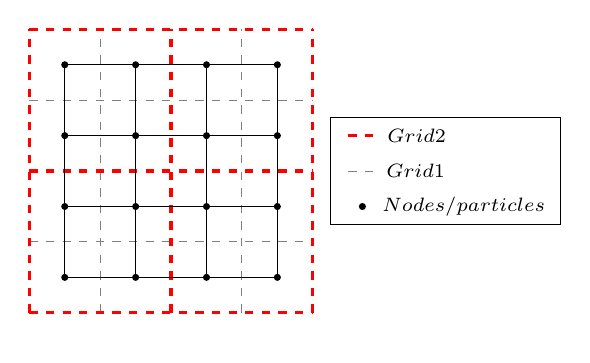
\begin{tikzpicture}[scale=0.9]
  \draw (0,0) --(3,0)--(3,3)--(0,3)--(0,0);
  \draw[white] (0.,0) -- (0,-0.8);
  %%% Grid 1
  \foreach \y in {-0.5,0.5,...,3.5} 
  \draw[dashed,gray] (-0.5,\y) -- (3.5,\y);
  \foreach \x in {-0.5,0.5,...,3.5} 
  \draw[dashed,gray] (\x,-0.5) -- (\x,3.5);
  %%% Grid 2
  \foreach \y in {-0.5,1.5,...,3.5} 
  \draw[dashed,Red,very thick] (-0.5,\y) -- (3.5,\y);
  \foreach \x in {-0.5,1.5,...,3.5} 
  \draw[dashed,Red,very thick] (\x,-0.5) -- (\x,3.5);
  \foreach \y in {0.,1.,...,3.} 
  \foreach \x in {0.,1.,...,3.} 
  \fill (\x,\y) circle(0.05);
  \foreach \y in {0.,1.,...,3.} 
  \draw (0,\y) -- (3.,\y);
  \foreach \x in {0.,1.,...,3.} 
  \draw (\x,0) -- (\x,3);
  \draw (3.75,0.75) rectangle (7.,2.25);
  \fill (4.2,1.) circle (0.05) node [right] {\scriptsize$ \: \: \text{Nodes / particles}$};
  \draw[dashed,gray] (4.,1.5) -- (4.4,1.5) node [right] {\scriptsize$\color{black} \text{Grid 1}$};
  \draw[dashed,very thick,Red] (4.,2.) -- (4.4,2.) node [right] {\scriptsize$\color{black} \text{Grid 2}$};
\end{tikzpicture}


%%% Local Variables:
%%% mode: latex
%%% TeX-master: "../manuscript"
%%% End:
}
  \caption{Geometry, loading and boundary conditions for the tensile impact problem on a two-dimensional elastic medium.}
  \label{fig:2D_planeStrain}
\end{figure}
The MPM and the DGMPM are compared to a $Q1$ finite element (bilinear approximation) solution coupled with a central difference explicit time integrator, computed with the code Cast3M \cite{Castem}.
Since no stability condition exists for the DGMPM scheme using RK2 time discretization for two-dimensional problems, we consider the DGMPM-Euler scheme in the remainder of the manuscript.
More specifically, the following simulations have been carried out by means of the CTU method.

The domain is discretized such that material points are equivalent to finite element nodes: $l\times l \equiv 28 \times 28$ particles and nodes. Moreover, two arbitrary grids are used for the DGMPM so that either one or four material points lie in every cells according to the situations depicted in figure \ref{fig:2D_planeStrain}\subref{subfig:2d_meshes}.
Figure \ref{fig:2delast_comparison} shows the isovalues of the longitudinal stress $\sigma_{11}$ in the two-dimensional medium at two different times with the traction force set to $\sigma^d=200\: Mpa$.
The two instants at which the solutions are depicted correspond to incident and reflected waves. In addition, the stress profiles along the bottom boundary of the domain are plotted in figures \ref{fig:elastlines}\subref{subfig:line_elast1} and \ref{fig:elastlines}\subref{subfig:line_elast2} for the same times.

Analogously to one-dimensional problems, the figures show that DGMPM solutions do not suffer from spurious oscillations while FEM and MPM one exhibits numerical noise.
\begin{figure}[h!]
  \centering
  \begin{tikzpicture}
  \begin{groupplot}[group style={group size=4 by 2,
      ylabels at=edge left, yticklabels at=edge left,
      horizontal sep=1.ex,
      vertical sep=2ex,},
    enlargelimits=0,
    xmin=0.,xmax=1., ymin=-0.,ymax=1.
    ,axis on top,scale only axis,xtick=\empty,ytick=\empty,width=0.2\linewidth,
    colorbar style={
      title style={
        font=\scriptsize,
        at={(1,.25)},
        anchor=north west
      },yticklabel style={font=\scriptsize}
      ,at={(current axis.south east)},anchor=south west
    }]
    %% FIRST ROW (time 1 = 3.5e-4s)
    %%% RANGE -2.0e7 -- 2.9e8
    \nextgroupplot[ylabel={$t=3.5\times 10^{-4} \:s$},title={(a) FEM}]\addplot graphics[xmin=0.,xmax=1., ymin=-0.,ymax=1.] {chapter4/pngFigures/fem_stress_115.png};
    \nextgroupplot[title={(b) DGMPM 1ppc}]\addplot graphics[xmin=-0.,xmax=1., ymin=-0.,ymax=1.] {chapter4/pngFigures/dgmpm1ppc_stress_115.png};
    \nextgroupplot[title={(c) DGMPM 4ppc}]\addplot graphics[xmin=-0.,xmax=1., ymin=-0.,ymax=1.] {chapter4/pngFigures/dgmpm4ppc_stress_115.png};
    \nextgroupplot[title={(d) MPM 1ppc},
    colorbar,colorbar style={
      title= {$\sigma_{11}\: (MPa)$},
      ytick={-5.7e-2,2.e-1,2.9e-1},
      yticklabels={-57,200,290},
    }]
    \addplot[scatter,scatter src=y,mark size=0.pt] coordinates {(0.,-5.7e-2) (0.,2.9e-1)};% Fake extreme values to fix scale
    \addplot graphics[xmin=-0.,xmax=1., ymin=-0.,ymax=1.] {chapter4/pngFigures/mpm_stress_115.png};

    %% SECOND ROW (time 2 =1.e-3s)
    %%% RANGE -4.4e7 -- 4.2e8
    \nextgroupplot[ylabel={$t=1.0\times 10^{-3} \:s$}]\addplot graphics[xmin=0.,xmax=1., ymin=-0.,ymax=1.] {chapter4/pngFigures/fem_stress_338.png};
    \nextgroupplot[]\addplot graphics[xmin=-0.,xmax=1., ymin=-0.,ymax=1.] {chapter4/pngFigures/dgmpm1ppc_stress_338.png};
    \nextgroupplot[]\addplot graphics[xmin=-0.,xmax=1., ymin=-0.,ymax=1.] {chapter4/pngFigures/dgmpm4ppc_stress_338.png};
    \nextgroupplot[colorbar,colorbar style={
      title= {$\sigma_{11}\: (MPa)$},
      ytick={-4.3e-2,2.e-1,4.8e-1},
      yticklabels={-43,200,480},
    }]
    \addplot[scatter,scatter src=y,mark size=0.pt] coordinates {(0.,-4.3e-2) (0.,4.8e-1)};% Fake extreme values to fix scale
    \addplot graphics[xmin=-0.,xmax=1., ymin=-0.,ymax=1.] {chapter4/pngFigures/mpm_stress_338.png};
    
  \end{groupplot}
\end{tikzpicture}



%%% Local Variables:
%%% mode: latex
%%% TeX-master: "../mainManuscript"
%%% End:

  \caption{Isovalues of longitudinal stress $\sigma_{11}$ solution of the tensile impact problem in a two-dimensional elastic medium. Comparison between FEM (CFL=0.9), DGMPM-CTU using 1ppc (CFL=1) or 4ppc (CFL=0.23), and MPM using 1ppc (CFL=0.7).}
  \label{fig:2delast_comparison}
\end{figure}
The decrease in the CFL number involved by 4ppc yields a less accurate resolution of the jump discontinuity carried by the longitudinal pressure wave than for 1ppc, which captures the incident right-going discontinuity (see figure \ref{fig:elastlines}\subref{subfig:line_elast1}).
Next, the interaction of shear and pressure waves traveling in the medium leads to a curved stress profile upstream of the discontinuity that is captured differently by all methods.  
\begin{figure}[h!]
  {\phantomsubcaption \label{subfig:line_elast1}}
  {\phantomsubcaption \label{subfig:line_elast2}}
  \begin{tikzpicture}
  \begin{groupplot}[group style={group size=2 by 1,
ylabels at=edge left, yticklabels at=edge left,horizontal sep=3.ex,
xticklabels at=edge bottom,xlabels at=edge bottom},
ymajorgrids=true,xmajorgrids=true,ylabel=$\sigma_{12} \: (Pa)$,
axis on top,scale only axis,width=0.4\linewidth, every x tick scale label/.style={at={(xticklabel* cs:1.05,0.75cm)},anchor=near yticklabel},ymin=-0.5e6,ymax=.5e9]
\nextgroupplot[ylabel=$\sigma_{11} (Pa)$,xlabel=$x (m)$]
\addplot[Red,very thick,no markers] table[x=Points:0,y=S11] {chapter4/csvFiles/2delast_fem_115.csv};
\addplot[Blue,very thick,mark=+,only marks,mark size=3pt] table[x=Points:0,y=stress_11] {chapter4/csvFiles/2delast_ctu1ppc_115.csv};
\addplot[Purple,very thick,mark=square*,only marks] table[x=Points:0,y=stress_11] {chapter4/csvFiles/2delast_ctu4ppc_115.csv};
\addplot[Orange,very thick,mark=x,only marks,mark size=3pt] table[x=Points:0,y=mpm_S11] {chapter4/csvFiles/2delast_mpm_115.csv};

\nextgroupplot[legend style={at={($(0.12,-0.35)+(0.9cm,1cm)$)},legend columns=2},xlabel=$x (m)$]
\addplot[Red,very thick,no markers] table[x=Points:0,y=S11] {chapter4/csvFiles/2delast_fem_338.csv};
\addplot[Blue,very thick,mark=+,only marks,mark size=3pt] table[x=Points:0,y=stress_11] {chapter4/csvFiles/2delast_ctu1ppc_338.csv};
\addplot[Purple,very thick,mark=square*,only marks] table[x=Points:0,y=stress_11] {chapter4/csvFiles/2delast_ctu4ppc_338.csv};
\addplot[Orange,very thick,mark=x,only marks,mark size=3pt] table[x=Points:0,y=mpm_S11] {chapter4/csvFiles/2delast_mpm_338.csv};
\addlegendentry{fem}
\addlegendentry{ctu 1ppc}
\addlegendentry{ctu 4ppc}
\addlegendentry{mpm}
   
  \end{groupplot}
\end{tikzpicture}


%%% Local Variables:
%%% mode: latex
%%% TeX-master: "../../mainManuscript"
%%% End:




































%%% Local Variables:
%%% mode: latex
%%% TeX-master: "../../mainManuscript"
%%% End:

  \caption{Evolution of longitudinal stress $\sigma_{11}$ along the bottom boundary of the elastic square plate. Comparison between FEM (CFL=0.9), DGMPM-CTU using 1ppc (CFL=1) or 4ppc (CFL=0.23), and MPM using 1ppc (CFL=0.7).}
  \label{fig:elastlines}
\end{figure}
On the other hand, the cylindrical profile of the longitudinal stress is quite well described by FEM and DGMPM with 1ppc, even after reflection of the fixed boundary as can be seen in figure \ref{fig:2delast_comparison}. The smoothness of DGMPM solutions using 4ppc and the oscillations in MPM results however prevent to distinguish this structure.

Figure \ref{fig:elastlines}\subref{subfig:line_elast2} also shows that the stress level on the right boundary of the domain differs from on method to another. Furthermore, MPM and FEM solutions after the passage of the reflected waves oscillate a lot compared to these of DGMPM schemes. In particular, the stress levels greatly differ after the reflection of the pressure wave.


%%% Local Variables:
%%% mode: latex
%%% TeX-master: "../mainManuscript"
%%% End:


\subsection{Plane strain problem -- Elastoplasticity}
\label{subsec:ep_planestrain}
The above solid is now supposed made of an elastic-plastic material with linear isotropic hardening. A tensile impact is still considered on the bottom left part of the domain, as depicted in figure \ref{fig:2D_planeStrain}\subref{subfig:2D_problem}, with the traction force $\sigma^d=2\sigma^y$ so that plastic flow occurs. A comparison between FEM (Cast3M Drexus), MPM and DGMPM using either one or four particles per elements is made on the equivalent plastic strain $p$, similar observation as above being made on the longitudinal stress $\sigma_{11}$.
The computation of intercell fluxes within the DGMPM is based on an elastic Riemann solver. Hence, the plastic flow is integrated by means of a radial return algorithm in every methods.

Figure \ref{fig:2dEP_comparison} shows FEM and DGMPM solutions before and after reflection of the longitudinal pressure wave on the right end of the domain. In addition, due to the large amplitude of equivalent plastic strain, MPM results for the same time steps are plotted separately in figure \ref{fig:2dEP_mpm}. A good agreement between FEM and DGMPM equivalent plastic strains can be seen in figure \ref{fig:2dEP_comparison}. 
\begin{figure}[h!]
  \centering
  \begin{tikzpicture}[scale=0.8]
  \begin{groupplot}[group style={group size=3 by 2,
      ylabels at=edge left, yticklabels at=edge left,
      horizontal sep=1.ex,
      vertical sep=2.ex,},
    enlargelimits=0,
    xmin=0.,xmax=1., ymin=-0.,ymax=1.
    ,axis on top,scale only axis,xtick=\empty,ytick=\empty,width=0.27\linewidth,
    colorbar style={
      title style={
        font=\scriptsize,
        at={(1,.5)},
        anchor=north west
      },yticklabel style={font=\scriptsize}
      ,at={(current axis.south east)},anchor=south west
    }]
    %% FIRST ROW (equivalent plastic strain)
    %%% RANGE 0 -- 4.3e-3
    \nextgroupplot[ylabel={$t=3.5\times 10^{-4} \:s$},title={(a) FEM}]\addplot graphics[xmin=0.,xmax=1., ymin=-0.,ymax=1.] {chapter4/pngFigures/ep_fem_p115.png};
    \nextgroupplot[title={(b) DGMPM 1ppc}]\addplot graphics[xmin=-0.,xmax=1., ymin=-0.,ymax=1.] {chapter4/pngFigures/ep_dgmpm1ppc_p115.png};
    \nextgroupplot[title={(c) DGMPM 4ppc},colorbar,colorbar style={
      title= {$p \: (\%)$},
      ytick={0.,4.3},
      yticklabels={0,0.43},
    }]
    \addplot[scatter,scatter src=y,mark size=0.pt] coordinates {(0.,0.) (0.,4.3)};% Fake extreme values to fix scale
    \addplot graphics[xmin=-0.,xmax=1., ymin=-0.,ymax=1.] {chapter4/pngFigures/ep_dgmpm4ppc_p115.png};
    %% THIRD ROW (equivalent plastic strain)
    %%% RANGE 0 -- 2.e-2
    \nextgroupplot[ylabel={$t=1.0\times 10^{-3} \:s$}]\addplot graphics[xmin=0.,xmax=1., ymin=-0.,ymax=1.] {chapter4/pngFigures/ep_fem_p338.png};
    \nextgroupplot[]\addplot graphics[xmin=-0.,xmax=1., ymin=-0.,ymax=1.] {chapter4/pngFigures/ep_dgmpm1ppc_p338.png};
    \nextgroupplot[colorbar,colorbar style={
      title= {$p \: (\%)$},
      ytick={0.,2.},
      yticklabels={0,2},
    }]
    \addplot[scatter,scatter src=y,mark size=0.pt] coordinates {(0.,0.) (0.,2.)};% Fake extreme values to fix scale
    \addplot graphics[xmin=-0.,xmax=1., ymin=-0.,ymax=1.] {chapter4/pngFigures/ep_dgmpm4ppc_p338.png};
  \end{groupplot}
\end{tikzpicture}



%%% Local Variables:
%%% mode: latex
%%% TeX-master: "../mainManuscript"
%%% End:
  \caption{Isovalues of equivalent plastic strain $p$ in an elastic-plastic plate linear isotropic hardening material at two different times. Comparison between FEM ($CFL=0.9$), DGMPM using 1ppc ($CFL=1$) and DGMP using 4ppc ($CFL=0.23$) solutions.}
  \label{fig:2dEP_comparison}
\end{figure}
\begin{figure}[h!]
  \centering
  \begin{tikzpicture}
  \begin{groupplot}[group style={group size=2 by 1,
      ylabels at=edge left, yticklabels at=edge left,
      horizontal sep=4.ex,
      vertical sep=2ex,},
    enlargelimits=0,
    xmin=0.,xmax=1., ymin=-0.,ymax=1.
    ,axis on top,scale only axis,xtick=\empty,ytick=\empty,width=0.27\linewidth,
    colorbar style={
      title style={
        font=\scriptsize,
        at={(1,.5)},
        anchor=north west
      },yticklabel style={font=\scriptsize}
      ,at={(current axis.south east)},anchor=south west
    }]
    %% FIRST ROW (first stress sigma11)
    
    % \nextgroupplot[title={(a) MPM results at time $t=3.5e-4 \:s$},
    % colorbar,colorbar style={
    %   title= {$\sigma_{11}\: (MPa)$},
    %   ytick={-0.27,8,9.2},
    %   yticklabels={-27,800,920},
    % }]
    % \addplot[scatter,scatter src=y,mark size=0.pt] coordinates {(0.,-0.27) (0.,9.2)};% Fake extreme values to fix scale
    % \addplot graphics[xmin=-0.,xmax=1., ymin=-0.,ymax=1.] {chapter4/pngFigures/ep_mpm_stress115.png};
    
    % \nextgroupplot[title={(b) MPM results at time $t=1.0e-3 \:s$},
    % colorbar,colorbar style={
    %   title= {$\sigma_{11}\: (MPa)$},
    %   ytick={-0.210,0.8,1.4},
    %   yticklabels={-210,800,1.4e3},
    % }]
    % \addplot[scatter,scatter src=y,mark size=0.pt] coordinates {(0.,-0.210) (0.,1.4)};% Fake extreme values to fix scale
    % \addplot graphics[xmin=-0.,xmax=1., ymin=-0.,ymax=1.] {chapter4/pngFigures/ep_mpm_stress338.png};
    
    %% SECOND ROW (first plastic strain epsp11)
    % \nextgroupplot[
    % colorbar,colorbar style={
    %   title= {$\eps^p_{11}$},
    %   ytick={-2.6,9.5},
    %   yticklabels={-2.6e-3,9.5e-3},
    % }]
    % \addplot[scatter,scatter src=y,mark size=0.pt] coordinates {(0.,-2.6) (0.,9.5)};% Fake extreme values to fix scale
    % \addplot graphics[xmin=-0.,xmax=1., ymin=-0.,ymax=1.] {chapter4/pngFigures/ep_mpm_epsp115.png};
    
    % \nextgroupplot[
    % colorbar,colorbar style={
    %   title= {$\eps^p_{11}$},
    %   ytick={-0.42,2.5},
    %   yticklabels={-4.2e-3,2.5e-2},
    % }]
    % \addplot[scatter,scatter src=y,mark size=0.pt] coordinates {(0.,-0.42) (0.,2.5)};% Fake extreme values to fix scale
    % \addplot graphics[xmin=-0.,xmax=1., ymin=-0.,ymax=1.] {chapter4/pngFigures/ep_mpm_epsp338.png};
    
    %% THIRD ROW (equivalent plastic strain)
    \nextgroupplot[title={(a) time $t=3.5e-4 \:s$}] \addplot graphics[xmin=-0.,xmax=1., ymin=-0.,ymax=1.] {chapter4/pngFigures/ep_mpm_p115.png};
    
    \nextgroupplot[title={(b) time $t=1.0e-3 \:s$},
    colorbar,colorbar style={
      title= {$p \: (\%)$},
      ytick={0,3.1},
      yticklabels={0,3.1},
    }]
    \addplot[scatter,scatter src=y,mark size=0.pt] coordinates {(0.,0) (0.,3.1)};% Fake extreme values to fix scale
    \addplot graphics[xmin=-0.,xmax=1., ymin=-0.,ymax=1.] {chapter4/pngFigures/ep_mpm_p338.png};
   
  \end{groupplot}
\end{tikzpicture}



%%% Local Variables:
%%% mode: latex
%%% TeX-master: "../mainManuscript"
%%% End:
  \caption{MPM isovalues of plastic strain $p$ in an elastic-plastic plate made of a linear isotropic hardening material at two different times ($CFL=0.7$).}
  \label{fig:2dEP_mpm}
\end{figure}
Nevertheless, a concentration of plastic strains occurs at the interface between loaded and traction free parts of the left boundary of the domain in DGMPM solutions. 
Such concentrations in the high gradients region can also be seen in MPM solutions depicted in figure \ref{fig:2dEP_mpm} so that this phenomenon seems to be a geometric effect arrising due to the space discretization rather than to numerical methods themselves.
%% Also plot stress
% \begin{figure}[h!]
%   \centering
%   \begin{tikzpicture}
  \begin{groupplot}[group style={group size=3 by 3,
      ylabels at=edge left, yticklabels at=edge left,
      horizontal sep=1.ex,
      vertical sep=5ex,},
    enlargelimits=0,
    xmin=0.,xmax=1., ymin=-0.,ymax=1.
    ,axis on top,scale only axis,xtick=\empty,ytick=\empty,width=0.27\linewidth,
    colorbar style={
      title style={
        font=\scriptsize,
        at={(1,.5)},
        anchor=north west
      },yticklabel style={font=\scriptsize}
      ,at={(current axis.south east)},anchor=south west
    }]
    %% FIRST ROW (first stress sigma11)
    %%% RANGE -4.8e7 -- 1.1e9
    \nextgroupplot[title={(a) FEM}]\addplot graphics[xmin=0.,xmax=1., ymin=-0.,ymax=1.] {chapter4/pngFigures/ep_fem_stress77.png};
    \nextgroupplot[title={(b) DGMPM 1ppc}]\addplot graphics[xmin=-0.,xmax=1., ymin=-0.,ymax=1.] {chapter4/pngFigures/ep_dgmpm1ppc_stress77.png};
    \nextgroupplot[title={(c) DGMPM 4ppc},
    colorbar,colorbar style={
      title= {$\sigma_{11}\: (MPa)$},
      ytick={-0.048,1.1},
      yticklabels={-48,1.1e3},
    }]
    \addplot[scatter,scatter src=y,mark size=0.pt] coordinates {(0.,-0.048) (0.,1.1)};% Fake extreme values to fix scale
    \addplot graphics[xmin=-0.,xmax=1., ymin=-0.,ymax=1.] {chapter4/pngFigures/ep_dgmpm4ppc_stress77.png};
    
    %% SECOND ROW (first plastic strain epsp11)
    %%% RANGE -4.3e-5 -- 3.9e-3
    \nextgroupplot[]\addplot graphics[xmin=0.,xmax=1., ymin=-0.,ymax=1.] {chapter4/pngFigures/ep_fem_epsp77.png};
    \nextgroupplot[]\addplot graphics[xmin=-0.,xmax=1., ymin=-0.,ymax=1.] {chapter4/pngFigures/ep_dgmpm1ppc_epsp77.png};
    \nextgroupplot[colorbar,colorbar style={
      title= {$\eps^p_{11}$},
      ytick={-0.043,3.9},
      yticklabels={-4.3e-5,3.9e-3},
    }]
    \addplot[scatter,scatter src=y,mark size=0.pt] coordinates {(0.,-0.043) (0.,3.9)};% Fake extreme values to fix scale
    \addplot graphics[xmin=-0.,xmax=1., ymin=-0.,ymax=1.] {chapter4/pngFigures/ep_dgmpm4ppc_epsp77.png};
    
    %% THIRD ROW (equivalent plastic strain)
    %%% RANGE 0 -- 4.3e-3
    \nextgroupplot[]\addplot graphics[xmin=0.,xmax=1., ymin=-0.,ymax=1.] {chapter4/pngFigures/ep_fem_p77.png};
    \nextgroupplot[]\addplot graphics[xmin=-0.,xmax=1., ymin=-0.,ymax=1.] {chapter4/pngFigures/ep_dgmpm1ppc_p77.png};
    \nextgroupplot[colorbar,colorbar style={
      title= {$p$},
      ytick={0.,4.3},
      yticklabels={0,4.3e-3},
    }]
    \addplot[scatter,scatter src=y,mark size=0.pt] coordinates {(0.,0.) (0.,4.3)};% Fake extreme values to fix scale
    \addplot graphics[xmin=-0.,xmax=1., ymin=-0.,ymax=1.] {chapter4/pngFigures/ep_dgmpm4ppc_p77.png};
  \end{groupplot}
\end{tikzpicture}



%%% Local Variables:
%%% mode: latex
%%% TeX-master: "../mainManuscript"
%%% End:
%   \caption{Isovalues of longitudinal stress $\sigma_{11}$ and equivalent plastic strain $p$ in an elastic-plastic plate linear isotropic hardening material at time $t=3.5e-4 \:s$. Comparison between FEM ($CFL=0.9$), DGMPM using 1ppc ($CFL=1$) and DGMP using 4ppc ($CFL=0.23$) solutions.}
%   \label{fig:2dEP_comparison1}
% \end{figure}
% \begin{figure}[h!]
%   \centering
%   \begin{tikzpicture}
  \begin{groupplot}[group style={group size=3 by 2,
      ylabels at=edge left, yticklabels at=edge left,
      horizontal sep=1.ex,
      vertical sep=2.ex,},
    enlargelimits=0,
    xmin=0.,xmax=1., ymin=-0.,ymax=1.
    ,axis on top,scale only axis,xtick=\empty,ytick=\empty,width=0.27\linewidth,
    colorbar style={
      title style={
        font=\scriptsize,
        at={(1,.5)},
        anchor=north west
      },yticklabel style={font=\scriptsize}
      ,at={(current axis.south east)},anchor=south west
    }]
    %% FIRST ROW (first stress sigma11)
    %%% RANGE -7.2e7 -- 1.1e9
    \nextgroupplot[title={(a) FEM}]\addplot graphics[xmin=0.,xmax=1., ymin=-0.,ymax=1.] {chapter4/pngFigures/ep_fem_stress338.png};
    \nextgroupplot[title={(b) DGMPM 1ppc}]\addplot graphics[xmin=-0.,xmax=1., ymin=-0.,ymax=1.] {chapter4/pngFigures/ep_dgmpm1ppc_stress338.png};
    \nextgroupplot[title={(c) DGMPM 4ppc},
    colorbar,colorbar style={
      title= {$\sigma_{11}\: (MPa)$},
      ytick={-0.73,8,8.9},
      yticklabels={-73,800,870},
    }]
    \addplot[scatter,scatter src=y,mark size=0.pt] coordinates {(0.,-0.73) (0.,8.9)};% Fake extreme values to fix scale
    \addplot graphics[xmin=-0.,xmax=1., ymin=-0.,ymax=1.] {chapter4/pngFigures/ep_dgmpm4ppc_stress338.png};
    
    %% SECOND ROW (first plastic strain epsp11)
    %%% RANGE -3.2e-5 -- 1.7e-2
    % \nextgroupplot[]\addplot graphics[xmin=0.,xmax=1., ymin=-0.,ymax=1.] {chapter4/pngFigures/ep_fem_epsp338.png};
    % \nextgroupplot[]\addplot graphics[xmin=-0.,xmax=1., ymin=-0.,ymax=1.] {chapter4/pngFigures/ep_dgmpm1ppc_epsp338.png};
    % \nextgroupplot[colorbar,colorbar style={
    %   title= {$\eps^p_{11}\cdot 10^{-2}$},
    %   ytick={-0.0032,1.7},
    %   yticklabels={-3.2e-5,1.7e-2},
    % }]
    % \addplot[scatter,scatter src=y,mark size=0.pt] coordinates {(0.,-0.0032) (0.,1.7)};% Fake extreme values to fix scale
    % \addplot graphics[xmin=-0.,xmax=1., ymin=-0.,ymax=1.] {chapter4/pngFigures/ep_dgmpm4ppc_epsp338.png};
      
    %% THIRD ROW (equivalent plastic strain)
    %%% RANGE 0 -- 2.e-2
    \nextgroupplot[]\addplot graphics[xmin=0.,xmax=1., ymin=-0.,ymax=1.] {chapter4/pngFigures/ep_fem_p338.png};
    \nextgroupplot[]\addplot graphics[xmin=-0.,xmax=1., ymin=-0.,ymax=1.] {chapter4/pngFigures/ep_dgmpm1ppc_p338.png};
    \nextgroupplot[colorbar,colorbar style={
      title= {$p \: (\%)$},
      ytick={0.,2.},
      yticklabels={0,2},
    }]
    \addplot[scatter,scatter src=y,mark size=0.pt] coordinates {(0.,0.) (0.,2.)};% Fake extreme values to fix scale
    \addplot graphics[xmin=-0.,xmax=1., ymin=-0.,ymax=1.] {chapter4/pngFigures/ep_dgmpm4ppc_p338.png};
  \end{groupplot}
\end{tikzpicture}



%%% Local Variables:
%%% mode: latex
%%% TeX-master: "../mainManuscript"
%%% End:
%   \caption{Isovalues of longitudinal stress $\sigma_{11}$ and equivalent plastic strain $p$ in an elastic-plastic plate linear isotropic hardening material at time $t=1.0e-3 \:s$. Comparison between FEM ($CFL=0.9$), DGMPM using 1ppc ($CFL=1$) and DGMP using 4ppc ($CFL=0.23$) solutions.}
%   \label{fig:2dEP_comparison2}
% \end{figure}
% \begin{figure}[h!]
%   \centering
%   \begin{tikzpicture}
  \begin{groupplot}[group style={group size=2 by 2,
      ylabels at=edge left, yticklabels at=edge left,
      horizontal sep=18.ex,
      vertical sep=2ex,},
    enlargelimits=0,
    xmin=0.,xmax=1., ymin=-0.,ymax=1.
    ,axis on top,scale only axis,xtick=\empty,ytick=\empty,width=0.25\linewidth,
    colorbar style={
      title style={
        font=\scriptsize,
        at={(1,.5)},
        anchor=north west
      },yticklabel style={font=\scriptsize}
      ,at={(current axis.south east)},anchor=south west
    }]
    %% FIRST ROW (first stress sigma11)
    
    \nextgroupplot[title={(a) MPM results at time $t=3.5e-4 \:s$},
    colorbar,colorbar style={
      title= {$\sigma_{11}\: (MPa)$},
      ytick={-0.27,8,9.2},
      yticklabels={-27,800,920},
    }]
    \addplot[scatter,scatter src=y,mark size=0.pt] coordinates {(0.,-0.27) (0.,9.2)};% Fake extreme values to fix scale
    \addplot graphics[xmin=-0.,xmax=1., ymin=-0.,ymax=1.] {chapter4/pngFigures/ep_mpm_stress115.png};
    
    \nextgroupplot[title={(b) MPM results at time $t=1.0e-3 \:s$},
    colorbar,colorbar style={
      title= {$\sigma_{11}\: (MPa)$},
      ytick={-0.210,0.8,1.4},
      yticklabels={-210,800,1.4e3},
    }]
    \addplot[scatter,scatter src=y,mark size=0.pt] coordinates {(0.,-0.210) (0.,1.4)};% Fake extreme values to fix scale
    \addplot graphics[xmin=-0.,xmax=1., ymin=-0.,ymax=1.] {chapter4/pngFigures/ep_mpm_stress338.png};
    
    %% SECOND ROW (first plastic strain epsp11)
    % \nextgroupplot[
    % colorbar,colorbar style={
    %   title= {$\eps^p_{11}$},
    %   ytick={-2.6,9.5},
    %   yticklabels={-2.6e-3,9.5e-3},
    % }]
    % \addplot[scatter,scatter src=y,mark size=0.pt] coordinates {(0.,-2.6) (0.,9.5)};% Fake extreme values to fix scale
    % \addplot graphics[xmin=-0.,xmax=1., ymin=-0.,ymax=1.] {chapter4/pngFigures/ep_mpm_epsp115.png};
    
    % \nextgroupplot[
    % colorbar,colorbar style={
    %   title= {$\eps^p_{11}$},
    %   ytick={-0.42,2.5},
    %   yticklabels={-4.2e-3,2.5e-2},
    % }]
    % \addplot[scatter,scatter src=y,mark size=0.pt] coordinates {(0.,-0.42) (0.,2.5)};% Fake extreme values to fix scale
    % \addplot graphics[xmin=-0.,xmax=1., ymin=-0.,ymax=1.] {chapter4/pngFigures/ep_mpm_epsp338.png};
    
    %% THIRD ROW (equivalent plastic strain)
    \nextgroupplot[
    colorbar,colorbar style={
      title= {$p \: (\%)$},
      ytick={-0.,1.1},
      yticklabels={0,1.1},
    }]
    \addplot[scatter,scatter src=y,mark size=0.pt] coordinates {(0.,0.) (0.,1.1)};% Fake extreme values to fix scale
    \addplot graphics[xmin=-0.,xmax=1., ymin=-0.,ymax=1.] {chapter4/pngFigures/ep_mpm_p115.png};
    
    \nextgroupplot[
    colorbar,colorbar style={
      title= {$p \: (\%)$},
      ytick={0,3.1},
      yticklabels={0,3.1},
    }]
    \addplot[scatter,scatter src=y,mark size=0.pt] coordinates {(0.,0) (0.,3.1)};% Fake extreme values to fix scale
    \addplot graphics[xmin=-0.,xmax=1., ymin=-0.,ymax=1.] {chapter4/pngFigures/ep_mpm_p338.png};
   
  \end{groupplot}
\end{tikzpicture}



%%% Local Variables:
%%% mode: latex
%%% TeX-master: "../mainManuscript"
%%% End:
%   \caption{Isovalues of MPM longitudinal stress $\sigma_{11}$ and plastic strain $p$ in an elastic-plastic plate made of a linear isotropic hardening material at two different times.}
%   \label{fig:2dEP_mpm}
% \end{figure}





%%% Local Variables:
%%% mode: latex
%%% TeX-master: "../mainManuscript"
%%% End:

\section{Large strain framework}
\label{sec:he_simulations}
%The DGMPM is now applied to problems involving finite deformations in hyperelastic solids in order to see the behavior of the method.
\subsection{Plane wave in a one-dimensional hyperelastic medium}
\label{subsec:he_planewave}

Parameters + 100 elems
% CFL=0.5
% NTmaxi = 300
% length = 6.0
% ppc=1
% Nelem = 100
% E = 2.0e11
% Sigy = 400.0e6
% rho = 7800.0
% nu = 0.3
% lamb = (E*nu)/((1+nu)*(1.-2.*nu))
% mu = E/(2.*(1.+nu))
% C=lamb+2.*mu
% c=np.sqrt(C/rho)

% factor=1.
% timeOut = 1.*length/c
% t_order=1
% timeUnload = 2*timeOut

% sigd = -50.*Sigy
% v0=0.*Sigy/(rho*c)
% algo = 'USL'
% update_position=False
% mpm_mapping=True
% limit=-1
\subsection{Compression impact on a SVK medium}
\begin{figure}[h!]
  \centering
  {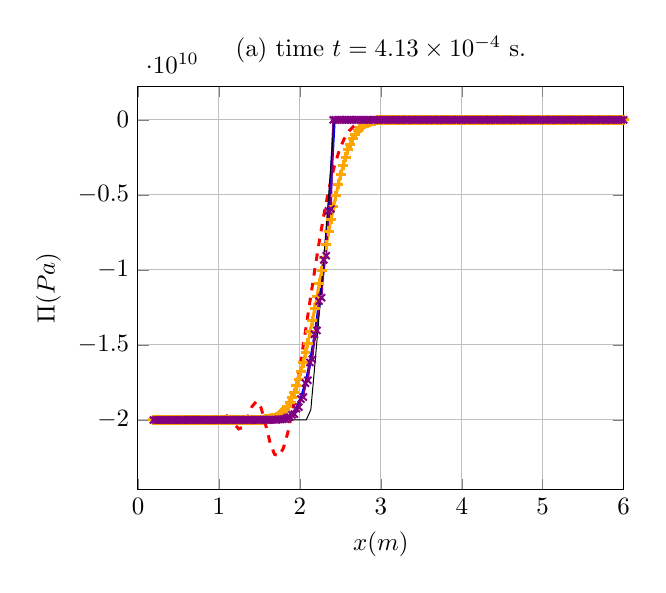
\begin{tikzpicture}[scale=0.9]
\begin{axis}[xlabel=$x (m)$,ylabel=$\Pi (Pa)$,ymajorgrids=true,xmajorgrids=true,legend pos= north west,title={(a) time $t = 4.13\times 10^{-4} $ s.},xmin=0.,xmax=6.]
\addplot[Red,very thick,mark=none,dashed] coordinates {(0.19429231621859985,-20006073362.447605) (0.2495994548763709,-19986671135.68456) (0.30488765068681783,-20009484715.95524) (0.3601633113593548,-19999667748.274166) (0.41543697640120997,-19998842866.58166) (0.4707103465207117,-19980025990.39316) (0.5259830952786003,-19989627937.11799) (0.5812473072363511,-20020206764.437843) (0.6365046678359781,-20022523341.484695) (0.6917664156560177,-19984739503.632847) (0.7470433887559937,-19921728114.52773) (0.8023244778509837,-19952983452.83056) (0.8575826939285168,-20056821377.767574) (0.9128086530876747,-20146050084.6668) (0.9680349361375865,-20050190867.486176) (1.0233128621502545,-19823950238.040665) (1.0786510045167328,-19674606159.17063) (1.1339854487171628,-19843113790.36482) (1.1892235807822906,-20263940048.802616) (1.2443383367011915,-20594817256.966568) (1.2994185016089512,-20471880070.475803) (1.3546192947754052,-19853505015.520443) (1.4100429786838058,-19090397669.844055) (1.4656431688200946,-18747034858.05499) (1.5212257963254028,-19197871377.32859) (1.5765578818799928,-20301404776.5628) (1.6315109848371214,-21504816953.264973) (1.6861313492294838,-22282313154.94336) (1.7405979869204695,-22404961380.902943) (1.795130755406773,-21893430427.415592) (1.8499225028760073,-20869875134.81481) (1.9051148450074284,-19464047060.06869) (1.9608005435269982,-17782564355.7729) (2.017033984688248,-15908990845.163458) (2.0738408016141867,-13912892750.116983) (2.1312243250448617,-11859055425.199602) (2.189169238000876,-9813911242.539871) (2.2476435755375186,-7847858230.686895) (2.306600325388235,-6032585818.503612) (2.365979745495297,-4433453223.385054) (2.425713123583109,-3098862125.3384204) (2.4857280382045643,-2050644755.106297) (2.5459543952157575,-1280061076.726812) (2.606329956594842,-751871062.4176673) (2.6668040860718976,-414991896.56532544) (2.7273390463695386,-215149915.47262502) (2.7879090497640973,-104798916.57747841) (2.8484979027936355,-47990190.44059481) (2.9090962327066574,-20674903.27414609) (2.9696990220743276,-8385318.738785009) (3.030303778267326,-3203330.0276726247) (3.0909093485437626,-1152979.973410103) (3.151515235363365,-391035.675115866) (3.2121212378932866,-124947.32039185325) (3.272727280203827,-37601.22723226968) (3.333333335378876,-10651.218022956937) (3.393939394466688,-2837.8277527031114) (3.454545454673374,-710.4571418349901) (3.515151515180682,-166.93032426436852) (3.5757575757638156,-36.758497954882436) (3.6363636363648877,-7.573117346901461) (3.6969696969699313,-1.456928594861368) (3.7575757575757986,-0.2611244553918368) (3.8181818181818246,-0.043490851945412384) (3.87878787878788,-0.006695498856200944) (3.9393939393939394,-0.000956499836600135) (4.0,-0.00011956247957501687) (4.0606060606060606,0.0) (4.121212121212121,0.0) (4.181818181818182,0.0) (4.242424242424242,0.0) (4.303030303030303,0.0) (4.363636363636363,0.0) (4.424242424242425,0.0) (4.484848484848485,0.0) (4.545454545454546,0.0) (4.606060606060606,0.0) (4.666666666666667,0.0) (4.7272727272727275,0.0) (4.787878787878788,0.0) (4.848484848484849,0.0) (4.909090909090909,0.0) (4.96969696969697,0.0) (5.03030303030303,0.0) (5.090909090909091,0.0) (5.151515151515151,0.0) (5.212121212121212,0.0) (5.2727272727272725,0.0) (5.333333333333334,0.0) (5.3939393939393945,0.0) (5.454545454545455,0.0) (5.515151515151516,0.0) (5.575757575757576,0.0) (5.636363636363637,0.0) (5.696969696969697,0.0) (5.757575757575758,0.0) (5.818181818181818,0.0) (5.878787878787879,0.0) (5.9393939393939394,0.0) (6.0,0.0) };
\addplot[Blue,very thick,mark=none,solid] coordinates {(0.19184481823272587,-20000746788.895386) (0.2472984593148165,-19999262845.167934) (0.3027550579515747,-20000799959.541138) (0.3582139828028267,-19999230865.055157) (0.4136744334611789,-20000901266.778095) (0.4691363798583578,-19999156573.758553) (0.5245991019399393,-20001058323.113438) (0.5800629488714097,-19999036648.84517) (0.635527105553384,-20001282242.769444) (0.6909922402572966,-19998864927.72781) (0.7464573416593343,-20001588390.21625) (0.8019234043904636,-19998632043.305565) (0.8573891369717147,-20001997440.71843) (0.9128559063396893,-19998324890.49686) (0.9683220513996212,-20002536843.16476) (1.023789388354951,-19997925908.97679) (1.0792557790732065,-20003242807.18485) (1.1347235977259633,-19997412156.041016) (1.1901900940405064,-20004162964.68389) (1.2456583458259118,-19996754091.63044) (1.3011248178858221,-20005359727.42986) (1.3565934830124184,-19995913073.930134) (1.412059799077113,-20006909700.64143) (1.467528884562971,-19994813482.07538) (1.5229949116205286,-20008792500.146915) (1.5784645009572125,-19992861846.161507) (1.63393029649414,-20009157097.143948) (1.689401269313731,-19983335218.807507) (1.7448693336716496,-19988556060.043617) (1.8003496405947086,-19915211430.44971) (1.8558399943620645,-19832464370.455975) (1.9113756485372175,-19565996896.830357) (1.9669788598771232,-19175060421.84385) (2.022726722440876,-18428718648.265965) (2.078678157853173,-17432821776.53043) (2.134949207911814,-15950492705.79851) (2.191612836208383,-14179637125.40624) (2.248793446466984,-11863860055.04507) (2.3065513731895595,-9241855726.717867) (2.365009406439806,-5893766492.953189) (2.4242424242424243,0.0) (2.484848484848485,0.0) (2.5454545454545454,0.0) (2.606060606060606,0.0) (2.666666666666667,0.0) (2.7272727272727275,0.0) (2.787878787878788,0.0) (2.8484848484848486,0.0) (2.909090909090909,0.0) (2.9696969696969697,0.0) (3.0303030303030303,0.0) (3.090909090909091,0.0) (3.1515151515151514,0.0) (3.2121212121212124,0.0) (3.272727272727273,0.0) (3.3333333333333335,0.0) (3.393939393939394,0.0) (3.4545454545454546,0.0) (3.515151515151515,0.0) (3.5757575757575757,0.0) (3.6363636363636367,0.0) (3.6969696969696972,0.0) (3.757575757575758,0.0) (3.8181818181818183,0.0) (3.878787878787879,0.0) (3.9393939393939394,0.0) (4.0,0.0) (4.0606060606060606,0.0) (4.121212121212121,0.0) (4.181818181818182,0.0) (4.242424242424242,0.0) (4.303030303030303,0.0) (4.363636363636363,0.0) (4.424242424242425,0.0) (4.484848484848485,0.0) (4.545454545454546,0.0) (4.606060606060606,0.0) (4.666666666666667,0.0) (4.7272727272727275,0.0) (4.787878787878788,0.0) (4.848484848484849,0.0) (4.909090909090909,0.0) (4.96969696969697,0.0) (5.03030303030303,0.0) (5.090909090909091,0.0) (5.151515151515151,0.0) (5.212121212121212,0.0) (5.2727272727272725,0.0) (5.333333333333334,0.0) (5.3939393939393945,0.0) (5.454545454545455,0.0) (5.515151515151516,0.0) (5.575757575757576,0.0) (5.636363636363637,0.0) (5.696969696969697,0.0) (5.757575757575758,0.0) (5.818181818181818,0.0) (5.878787878787879,0.0) (5.9393939393939394,0.0) (6.0,0.0) };
\addplot[Orange,very thick,mark=+,solid] coordinates {(0.18995525166111366,-19999912858.22518) (0.21763857805956868,-19999769787.88829) (0.24512208706281055,-19999595225.830395) (0.27282575705740886,-19999451694.173355) (0.3003071750929951,-19999276292.69227) (0.32801595744355366,-19999131832.277004) (0.3554953427946694,-19998955018.611973) (0.3832066011773739,-19998809148.97717) (0.4106846406234849,-19998630330.553932) (0.4383974367587157,-19998482551.158222) (0.46587453401796425,-19998301106.73408) (0.49358840901570517,-19998150889.20853) (0.5210648104045611,-19997966159.024174) (0.5487795002679247,-19997812938.436954) (0.5762553672290964,-19997624212.983093) (0.6039707041588833,-19997467377.749435) (0.6314461490108538,-19997273884.659058) (0.659162018895618,-19997112764.632294) (0.6866371235984735,-19996913653.070396) (0.7143534449920753,-19996747505.207943) (0.7418282717305508,-19996541826.930435) (0.7695449843941599,-19996369817.725258) (0.7970195819297244,-19996156503.688694) (0.8247366401192712,-19995977687.259945) (0.8522110478099802,-19995755518.23956) (0.8799284161209588,-19995568808.532024) (0.9074026665852393,-19995336377.560326) (0.9351203172698606,-19995140512.397816) (0.9625944382274981,-19994896175.737343) (0.9903123494081251,-19994689669.049244) (1.0177863650063577,-19994431479.734898) (1.0455045194632855,-19994212553.503006) (1.0729784512767135,-19993938160.470367) (1.1006968356268219,-19993704624.606678) (1.1281707034621382,-19993411064.120533) (1.1558893076415115,-19993159994.96435) (1.1833631302893026,-19992843029.618053) (1.2110819473987793,-19992569575.424583) (1.2385557436795793,-19992221110.35909) (1.2662747707021536,-19991913792.57851) (1.2937485620273468,-19991511992.659107) (1.3214678034398997,-19991135778.789246) (1.348941622020031,-19990611361.07096) (1.3766611027821543,-19990054404.717606) (1.4041350176396072,-19989191087.10363) (1.43185482298986,-19988120795.17056) (1.4593290140068589,-19986303943.14754) (1.4870493950945292,-19983836663.36228) (1.5145243372708168,-19979517453.333805) (1.5422459535049426,-19973584795.21019) (1.5697228130621068,-19963335295.939476) (1.5974472092249048,-19949696944.16045) (1.6249285708236694,-19926887514.67977) (1.6526589729400751,-19897960308.693275) (1.6801499595587883,-19851437924.117283) (1.7078923745712826,-19795437569.700573) (1.7354020457070085,-19708969482.813923) (1.7631664627875865,-19610053565.1548) (1.7907091203275556,-19463351503.24422) (1.8185104215571681,-19303209212.943596) (1.846106271632855,-19074774470.23491) (1.8739644155740336,-18835426807.336002) (1.9016391139595983,-18506490966.59541) (1.929578344685977,-18173408100.377052) (1.9573613220878685,-17731609002.064552) (1.9854084938213,-17296152224.080425) (2.013330410494915,-16737796934.560286) (2.041512798178765,-16198491879.856827) (2.069602736105936,-15529090279.041159) (2.097945774544229,-14891880186.885708) (2.1262287257995864,-14125409710.52269) (2.154753998432247,-13403375220.585518) (2.1832489573267595,-12561011287.379313) (2.211972566392059,-11773975414.023428) (2.24069126999827,-10882817742.279064) (2.2696225838776267,-10056933247.623539) (2.2985687962945347,-9148834985.540192) (2.327709541119762,-8315860661.742456) (2.356878766471977,-7426050359.213425) (2.3862225001407333,-6621710808.248219) (2.4156021007706037,-5786632187.628343) (2.4451342315442015,-5047407133.728801) (2.47470405839892,-4301249043.455953) (2.5044026660566034,-3659402379.111651) (2.5341363952031912,-3029346440.874573) (2.563974070845136,-2507081699.0016084) (2.593841384344465,-2008351349.8441858) (2.623788042880702,-1613201600.0153964) (2.6537575319704074,-1245972269.7087686) (2.6837837243855356,-969806805.9692637) (2.713826006898169,-719895044.9301026) (2.743905915736818,-542465644.1033932) (2.773996200748826,-386006963.2538726) (2.804109532245024,-281510641.82021976) (2.8342289849581657,-191643401.31466892) (2.8643614213299275,-135290962.20125788) (2.8944971613083075,-87983443.40475516) (2.924639617951817,-60153986.76079956) (2.9547837066305997,-37328498.31375421) (2.9849309849010037,-24733077.95371384) (3.015079001851262,-14631759.500679849) (3.045228409801474,-9402072.941124339) (3.0753781243862,-5298061.620119785) (3.105528396475034,-3304104.722537816) (3.1356787854200334,-1771954.9486091677) (3.1658293798711896,-1073279.4290237231) (3.195980015238912,-547296.2783473512) (3.226130720321594,-322187.11395850533) (3.2562814385751238,-156061.14816243792) (3.286432178602333,-89350.21257776454) (3.316582922528392,-41065.456399169176) (3.3467336727166184,-22880.71737255304) (3.3768844239662927,-9965.667379406394) (3.4070351768743565,-5407.004064866737) (3.437185930048142,-2228.6748053008914) (3.4673366836262214,-1178.1706413573809) (3.497487437265445,-458.856763768479) (3.527638190995354,-236.47913094118658) (3.5577889447381867,-86.87293189700003) (3.587939698499721,-43.6702853295511) (3.618090452263762,-15.102474825431294) (3.6482412060313454,-7.4089580622410764) (3.6783919597993746,-2.406673151344001) (3.7085427135680193,-1.1526420843380152) (3.7386934673367365,-0.35061697135328035) (3.768844221105552,-0.1639201594972483) (3.798994974874379,-0.04639024207509855) (3.8291457286432187,-0.02113266826488257) (3.8592964824120606,-0.005410202200769404) (3.8894472361809047,-0.002271687111925301) (3.9195979899497484,-0.00044835929840631247) (3.949748743718593,-0.00017934371936252516) (3.979899497487437,0.0) (4.010050251256281,0.0) (4.040201005025126,0.0) (4.0703517587939695,0.0) (4.100502512562814,0.0) (4.130653266331658,-5.9781239787508415e-05) (4.160804020100502,0.0) (4.190954773869347,0.0) (4.221105527638191,0.0) (4.251256281407035,0.0) (4.281407035175879,0.0) (4.311557788944723,0.0) (4.341708542713568,0.0) (4.371859296482412,0.0) (4.402010050251256,0.0) (4.4321608040201,-5.9781239787508415e-05) (4.4623115577889445,0.0) (4.492462311557789,0.0) (4.522613065326633,0.0) (4.552763819095477,0.0) (4.582914572864321,0.0) (4.613065326633166,0.0) (4.64321608040201,0.0) (4.673366834170854,0.0) (4.703517587939698,0.0) (4.733668341708542,0.0) (4.763819095477387,0.0) (4.793969849246231,0.0) (4.824120603015075,0.0) (4.8542713567839195,0.0) (4.884422110552763,0.0) (4.914572864321608,0.0) (4.944723618090452,0.0) (4.974874371859296,0.0) (5.005025125628141,0.0) (5.035175879396984,0.0) (5.065326633165829,0.0) (5.0954773869346734,0.0) (5.125628140703517,0.0) (5.155778894472362,0.0) (5.185929648241205,0.0) (5.21608040201005,0.0) (5.2462311557788945,0.0) (5.276381909547738,-5.9781239787508415e-05) (5.306532663316583,0.0) (5.3366834170854265,0.0) (5.366834170854271,0.0) (5.396984924623116,0.0) (5.427135678391959,0.0) (5.457286432160804,0.0) (5.487437185929648,0.0) (5.517587939698492,0.0) (5.547738693467337,0.0) (5.57788944723618,0.0) (5.608040201005025,0.0) (5.638190954773869,-5.9781239787508415e-05) (5.668341708542713,0.0) (5.698492462311558,0.0) (5.7286432160804015,0.0) (5.758793969849246,0.0) (5.788944723618091,0.0) (5.819095477386934,0.0) (5.849246231155779,0.0) (5.879396984924623,-5.9781239787508415e-05) (5.909547738693467,0.0) (5.939698492462312,0.0) (5.969849246231155,0.0) (6.0,0.0) };
\addplot[Purple,thick,mark=x,solid] coordinates {(0.19087078866902665,-19999455640.176197) (0.22071218292775385,-19999409659.864017) (0.2459924077656396,-20000077312.85232) (0.27597326522813487,-20000072009.997063) (0.3011894927456019,-19998950742.164944) (0.3311766255539742,-19998862763.515118) (0.3563962430072859,-19999589159.90041) (0.38636963567121163,-19999626165.686943) (0.41160234396465,-19998404877.00223) (0.4415609586628959,-19998270520.060898) (0.4668064289385858,-19999118873.727676) (0.49675180124731944,-19999202922.963924) (0.5220088990140508,-19997806766.43407) (0.5519428363462726,-19997618279.35031) (0.5772098159593475,-19998661098.62433) (0.6071336614902496,-19998800403.628937) (0.6324097933704171,-19997141589.490086) (0.6623248466555562,-19996887265.347076) (0.6876086367678674,-19998211885.709827) (0.7175157537096876,-19998418772.38764) (0.7428070060201625,-19996389972.392735) (0.7727071471896477,-19996053259.198273) (0.7980044513100885,-19997768502.897907) (0.8278981543338224,-19998060358.486023) (0.8532017639590902,-19995526549.26538) (0.8830898001721301,-19995084778.141758) (0.9083982334111295,-19997329243.71315) (0.9382809151671918,-19997729846.142517) (0.9635948605946703,-19994517924.97995) (0.9934728615949118,-19993940550.927967) (1.018790634157661,-19996893154.38264) (1.0486640867664065,-19997434481.72408) (1.0739868482392012,-19993319799.35868) (1.103856391967528,-19992566008.07375) (1.129182120960812,-19996459571.531334) (1.1590477257284901,-19997184225.495197) (1.1843781409943626,-19991872941.060112) (1.2142404634066721,-19990888423.449177) (1.2395730548989103,-19996027394.59501) (1.269431901039365,-19996991817.22908) (1.2947690752904193,-19990097771.00673) (1.3246251669949154,-19988810395.611206) (1.3499637385624637,-19995594394.611435) (1.3798167010879285,-19996873032.549503) (1.4051599499623135,-19987887684.922043) (1.4350106214725087,-19986201196.541973) (1.4603544495160277,-19995154760.05428) (1.4902022422851016,-19996842075.848194) (1.5155510581278278,-19985077422.35594) (1.5453969866641184,-19982845663.359066) (1.570745480163516,-19994550689.773247) (1.6005886999258214,-19996684108.793686) (1.625942792905406,-19980692933.116657) (1.6557845912583171,-19977385747.898075) (1.6811375441326768,-19990452521.34305) (1.7109768445952687,-19991936790.38711) (1.736337222388458,-19962562834.670414) (1.7661759691627483,-19954268934.61151) (1.7915371396346151,-19946636578.575214) (1.8213747099598598,-19938461812.41097) (1.8467537764093123,-19837157162.833206) (1.8765945013072705,-19804712010.78006) (1.9019952765295465,-19662159771.99237) (1.9318415620560758,-19612768170.56989) (1.9573086438181697,-19243797603.25251) (1.987170301328827,-19145197075.79308) (2.0127391582847944,-18606422582.842396) (2.042623150182732,-18474857956.820774) (2.068383513683698,-17546640829.370613) (2.0983030697861436,-17356604515.480618) (2.1243218125728434,-16168446386.224903) (2.154282226835199,-15957833195.666677) (2.1806765607592036,-14287253493.297613) (2.2106861953891266,-14032581607.352451) (2.2375256180290903,-12078287603.813477) (2.2675794640427664,-11846950370.664488) (2.2949840954789456,-9331938813.91532) (2.325083226953284,-9055544632.420107) (2.3531208903662257,-6074271277.8443) (2.3832414203422285,-5944142832.467713) (2.4120603015075375,0.0004184686785125597) (2.4422110552763816,0.0004184686785125597) (2.472361809045226,0.000717374877450103) (2.5025125628140703,0.000717374877450103) (2.5326633165829144,0.0001793437193625254) (2.5628140703517586,0.0001793437193625254) (2.5929648241206027,0.0005978123978750856) (2.6231155778894473,0.0005978123978750856) (2.6532663316582914,0.0005978123978750856) (2.6834170854271355,0.0005978123978750856) (2.7135678391959797,0.0006575936376625943) (2.743718592964824,0.0005978123978750856) (2.7738693467336684,0.0005380311580875769) (2.8040201005025125,0.0004782499183000683) (2.8341708542713566,0.0003586874387250511) (2.8643216080402008,0.0003586874387250511) (2.8944723618090453,0.00011956247957501691) (2.9246231155778895,0.00011956247957501691) (2.9547738693467336,0.0005380311580875769) (2.9849246231155777,0.0004782499183000683) (3.015075376884422,0.0005380311580875769) (3.0452261306532664,0.0005380311580875769) (3.0753768844221105,0.000717374877450103) (3.1055276381909547,0.000717374877450103) (3.135678391959799,0.0001793437193625254) (3.165829145728643,0.00011956247957501691) (3.1959798994974875,0.0005978123978750856) (3.2261306532663316,0.0005978123978750856) (3.2562814070351758,0.0004782499183000683) (3.28643216080402,0.0004782499183000683) (3.316582914572864,0.0002989061989375425) (3.3467336683417086,0.00023912495915003393) (3.3768844221105527,0.0005978123978750856) (3.407035175879397,0.0005380311580875769) (3.437185929648241,0.0004184686785125597) (3.467336683417085,0.0004184686785125597) (3.4974874371859297,0.0002989061989375425) (3.527638190954774,0.0002989061989375425) (3.557788944723618,5.978123978750844e-05) (3.587939698492462,5.978123978750844e-05) (3.618090452261306,0.00011956247957501691) (3.648241206030151,0.0) (3.678391959798995,0.0001793437193625254) (3.708542713567839,0.00011956247957501691) (3.738693467336683,0.0005978123978750856) (3.7688442211055273,0.0005978123978750856) (3.798994974874372,0.0) (3.829145728643216,-0.0001195624795750168) (3.85929648241206,0.0003586874387250511) (3.8894472361809043,0.0002989061989375425) (3.9195979899497484,0.0004782499183000683) (3.949748743718593,0.0004782499183000683) (3.979899497487437,0.00011956247957501691) (4.010050251256281,5.978123978750844e-05) (4.040201005025126,-0.00032879681883129597) (4.0703517587939695,-0.00032879681883129597) (4.100502512562814,0.0005978123978750856) (4.130653266331658,0.0005978123978750856) (4.160804020100502,0.0) (4.190954773869347,0.00011956247957501691) (4.221105527638191,0.0005978123978750856) (4.251256281407035,0.0005978123978750856) (4.281407035175879,0.00023912495915003393) (4.311557788944723,0.00023912495915003393) (4.341708542713568,-5.9781239787508415e-05) (4.371859296482412,-0.0001195624795750168) (4.402010050251256,0.0005978123978750856) (4.4321608040201,0.0005978123978750856) (4.4623115577889445,-0.00044835929840631247) (4.492462311557789,-0.00044835929840631247) (4.522613065326633,0.0004782499183000683) (4.552763819095477,0.0005380311580875769) (4.582914572864321,0.0001793437193625254) (4.613065326633166,0.00011956247957501691) (4.64321608040201,0.0005978123978750856) (4.673366834170854,0.0005380311580875769) (4.703517587939698,0.0006575936376625943) (4.733668341708542,0.0006575936376625943) (4.763819095477387,-0.00032879681883129597) (4.793969849246231,-0.00032879681883129597) (4.824120603015075,0.0005978123978750856) (4.8542713567839195,0.0005978123978750856) (4.884422110552763,-0.00029890619893754183) (4.914572864321608,-0.00029890619893754183) (4.944723618090452,0.0006575936376625943) (4.974874371859296,0.0005978123978750856) (5.005025125628141,-0.00032879681883129597) (5.035175879396984,-0.00032879681883129597) (5.065326633165829,0.00023912495915003393) (5.0954773869346734,0.00023912495915003393) (5.125628140703517,0.0003586874387250511) (5.155778894472362,0.0004184686785125597) (5.185929648241205,-0.00044835929840631247) (5.21608040201005,-0.00032879681883129597) (5.2462311557788945,0.0005978123978750856) (5.276381909547738,0.0005978123978750856) (5.306532663316583,0.00023912495915003393) (5.3366834170854265,0.00023912495915003393) (5.366834170854271,-0.00044835929840631247) (5.396984924623116,-0.0003885780586188042) (5.427135678391959,0.0003586874387250511) (5.457286432160804,0.0004184686785125597) (5.487437185929648,-0.0003885780586188042) (5.517587939698492,-0.00044835929840631247) (5.547738693467337,0.0005978123978750856) (5.57788944723618,0.0005978123978750856) (5.608040201005025,-0.00029890619893754183) (5.638190954773869,-0.00029890619893754183) (5.668341708542713,0.0006575936376625943) (5.698492462311558,0.0006575936376625943) (5.7286432160804015,-0.00017934371936252516) (5.758793969849246,-0.00017934371936252516) (5.788944723618091,-0.00032879681883129597) (5.819095477386934,-0.00032879681883129597) (5.849246231155779,0.0006575936376625943) (5.879396984924623,0.0006575936376625943) (5.909547738693467,-0.00032879681883129597) (5.939698492462312,-0.00032879681883129597) (5.969849246231155,0.0011358435559626649) (6.0,0.0007771561172376117) };
\addplot[black,thin,mark=none,solid] coordinates {(0.19184481823272587,-19999999999.99513) (0.2472984593148165,-19999999999.99513) (0.3027550579515747,-19999999999.99513) (0.3582139828028267,-19999999999.99513) (0.4136744334611789,-19999999999.99513) (0.4691363798583578,-19999999999.99513) (0.5245991019399393,-19999999999.99513) (0.5800629488714097,-19999999999.99513) (0.635527105553384,-19999999999.99513) (0.6909922402572966,-19999999999.99513) (0.7464573416593343,-19999999999.99513) (0.8019234043904636,-19999999999.99513) (0.8573891369717147,-19999999999.99513) (0.9128559063396893,-19999999999.99513) (0.9683220513996212,-19999999999.99513) (1.023789388354951,-19999999999.99513) (1.0792557790732065,-19999999999.99513) (1.1347235977259633,-19999999999.99513) (1.1901900940405064,-19999999999.99513) (1.2456583458259118,-19999999999.99513) (1.3011248178858221,-19999999999.99513) (1.3565934830124184,-19999999999.99513) (1.412059799077113,-19999999999.99513) (1.467528884562971,-19999999999.99513) (1.5229949116205286,-19999999999.99513) (1.5784645009572125,-19999999999.99513) (1.63393029649414,-19999999999.99513) (1.689401269313731,-19999999999.99513) (1.7448693336716496,-19999999999.99513) (1.8003496405947086,-19999999999.99513) (1.8558399943620645,-19999999999.99513) (1.9113756485372175,-19999999999.99513) (1.9669788598771232,-19999999999.99513) (2.022726722440876,-19999999999.99513) (2.078678157853173,-19999999999.99513) (2.134949207911814,-19320644756.027233) (2.191612836208383,-15934816130.431961) (2.248793446466984,-12317415446.21064) (2.3065513731895595,-8460847327.543606) (2.365009406439806,-4357551166.693738) (2.4242424242424243,-8.967185968126261e-05) (2.484848484848485,0.0) (2.5454545454545454,0.0) (2.606060606060606,0.0) (2.666666666666667,0.0) (2.7272727272727275,0.0) (2.787878787878788,0.0) (2.8484848484848486,0.0) (2.909090909090909,0.0) (2.9696969696969697,0.0) (3.0303030303030303,0.0) (3.090909090909091,0.0) (3.1515151515151514,0.0) (3.2121212121212124,0.0) (3.272727272727273,0.0) (3.3333333333333335,0.0) (3.393939393939394,0.0) (3.4545454545454546,0.0) (3.515151515151515,0.0) (3.5757575757575757,0.0) (3.6363636363636367,0.0) (3.6969696969696972,0.0) (3.757575757575758,0.0) (3.8181818181818183,0.0) (3.878787878787879,0.0) (3.9393939393939394,0.0) (4.0,0.0) (4.0606060606060606,0.0) (4.121212121212121,0.0) (4.181818181818182,0.0) (4.242424242424242,0.0) (4.303030303030303,0.0) (4.363636363636363,0.0) (4.424242424242425,0.0) (4.484848484848485,0.0) (4.545454545454546,0.0) (4.606060606060606,0.0) (4.666666666666667,0.0) (4.7272727272727275,0.0) (4.787878787878788,0.0) (4.848484848484849,0.0) (4.909090909090909,0.0) (4.96969696969697,0.0) (5.03030303030303,0.0) (5.090909090909091,0.0) (5.151515151515151,0.0) (5.212121212121212,0.0) (5.2727272727272725,0.0) (5.333333333333334,0.0) (5.3939393939393945,0.0) (5.454545454545455,0.0) (5.515151515151516,0.0) (5.575757575757576,0.0) (5.636363636363637,0.0) (5.696969696969697,0.0) (5.757575757575758,0.0) (5.818181818181818,0.0) (5.878787878787879,0.0) (5.9393939393939394,0.0) (6.0,0.0) };
%\legend{mpm,dgmpm,dgmpm 2ppc,dgmpm 2ppc (RK2),exact}
\end{axis}
\end{tikzpicture}
%%% Local Variables:
%%% mode: latex
%%% TeX-master: "../../mainManuscript"
%%% End:
}
  {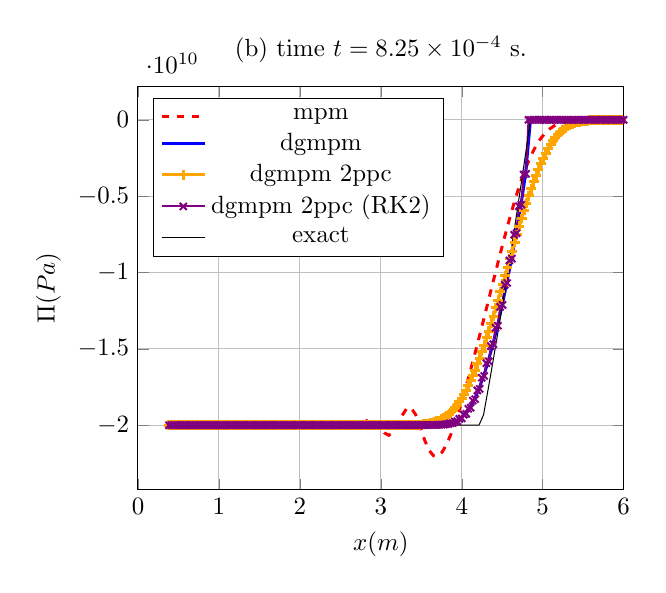
\begin{tikzpicture}[scale=0.9]
\begin{axis}[xlabel=$x (m)$,ylabel=$\Pi (Pa)$,ymajorgrids=true,xmajorgrids=true,legend pos= north west,title={(b) time $t = 8.25\times 10^{-4} $ s.},xmin=0.,xmax=6.]
\addplot[Red,very thick,mark=none,dashed] coordinates {(0.39037665296779944,-20003189832.924717) (0.4456826624098611,-19996503392.149483) (0.5009704081817377,-20002423865.30926) (0.5562477051357223,-19996663831.661327) (0.6115214671319547,-20001250436.505577) (0.6667916713890001,-19997098449.727352) (0.7220599841425713,-19999850425.379917) (0.7773261888093733,-19997733483.30031) (0.8325911169429844,-19998457405.552814) (0.8878545954294681,-19998172379.55476) (0.9431171523187737,-19997060791.85406) (0.9983786116645804,-19998515112.86419) (1.0536392800775984,-19996294129.02629) (1.1088991050268924,-19998580900.381916) (1.1641583617305475,-19995161992.177692) (1.2194170584909185,-19997783430.157677) (1.2746751455719256,-19995019664.29004) (1.3299325546069887,-19998356312.732986) (1.3851894014031947,-19995142276.615314) (1.440446120748,-19996033685.0159) (1.4957027682981452,-19992681848.43269) (1.5509590057181089,-19995837672.158688) (1.6062141479872896,-19996864692.176643) (1.6614684602296836,-19998537719.943672) (1.7167230488688772,-19992892483.20531) (1.7719789946782127,-19988038530.35165) (1.82723541951324,-19987907927.88097) (1.8824899297224313,-19997884231.884083) (1.9377410378048592,-20006998170.569366) (1.992990982052666,-20003291582.8411) (2.048244536261618,-19983116930.387775) (2.1035041139195854,-19964626538.336937) (2.158765380956268,-19971191190.943844) (2.2140194752544087,-20007300954.07061) (2.2692615892045946,-20043473199.570866) (2.3244985045254714,-20037918448.64995) (2.379745934071556,-19977514508.271114) (2.4350150949052325,-19902893223.128666) (2.4902990615797935,-19885086712.44862) (2.5455728359621737,-19964527399.680172) (2.600811231075641,-20101622922.07862) (2.6560125835853357,-20190890892.43871) (2.7112079396347393,-20137363487.620422) (2.7664442877571327,-19938059448.664787) (2.8217504532992774,-19706038716.735638) (2.877109241914055,-19611651838.0191) (2.932458181878787,-19766041902.035404) (2.987723764218724,-20124951487.09777) (3.0428699262610155,-20497282232.250183) (3.097928421241977,-20658341134.843044) (3.15299005677472,-20477314010.5783) (3.2081619712653873,-19983953129.284122) (3.2635139519321505,-19366282851.56678) (3.3190385147751815,-18907386953.67469) (3.3746434139264263,-18861004098.695183) (3.4301842919341103,-19308408173.791897) (3.4855254392177364,-20102759962.726917) (3.5405962301652343,-20963955609.67389) (3.595411641488975,-21639850979.945942) (3.650052623151561,-21998693237.441765) (3.704628748837566,-22021109583.9792) (3.759247233450719,-21748903217.199604) (3.8139972877359294,-21241666247.970295) (3.8689466345209116,-20554586606.16369) (3.9241440347720444,-19731428499.847054) (3.979623510165095,-18804636140.55174) (4.035408269046417,-17797719528.657604) (4.091513741202905,-16727844991.48753) (4.1479497215902805,-15607993683.041618) (4.204721795959992,-14448629306.539152) (4.26183222716596,-13258990180.139458) (4.31928044015377,-12048136541.240799) (4.377063202594848,-10825844231.278728) (4.4351745717483615,-9603375178.328075) (4.493605669962795,-8394083734.698876) (4.552344360413229,-7213744839.791666) (4.61137491678105,-6080434550.192567) (4.670677806323034,-5013788525.410298) (4.730229720485612,-4033546216.1358347) (4.790003973621545,-3157473637.7910213) (4.849971335735706,-2399009623.198169) (4.910101271027266,-1765197998.4938393) (4.9703634425016645,-1255518225.0189953) (5.030729253140749,-862026954.9625841) (5.0911731653358485,-570819752.9116776) (5.151673590028141,-364393886.3401778) (5.212213248266168,-224245701.4919938) (5.272779036564631,-133069828.57873616) (5.333361526088788,-76181815.88905498) (5.393954267233807,-42102378.65186526) (5.4545530573604495,-22476814.403691825) (5.515155282072059,-11599088.280085122) (5.575759385379125,-5789569.663655625) (5.636364479528455,-2796734.4204148627) (5.696970078102157,-1308178.1516057253) (5.757575924739028,-592841.2714692679) (5.818181889285784,-260605.75219605683) (5.878787907980832,-111756.925026151) (5.939393950560784,-48398.014397437015) (6.000000002859722,-25407.541372095384) };
\addplot[Blue,very thick,mark=none,solid] coordinates {(0.38401698079958846,-19999993425.18581) (0.4394706083791145,-19999974753.481766) (0.4949272641367282,-19999961717.61289) (0.5503861475694772,-19999942904.998543) (0.6058467157310151,-19999930217.40262) (0.6613085899995965,-19999911111.718575) (0.7167714966962511,-19999899028.369488) (0.7722352359338598,-19999879454.1201) (0.8276996549718213,-19999868268.3495) (0.8831646391924676,-19999848012.893536) (0.9386300959070943,-19999838073.78776) (0.9940959553211544,-19999816870.787548) (1.0495621569710856,-19999808605.328205) (1.105028656709029,-19999786114.244507) (1.160495412363306,-19999780054.698708) (1.2159623956589096,-19999755834.83223) (1.2714295751240139,-19999752653.273045) (1.3268969331110458,-19999726130.46261) (1.382364444349215,-19999726682.80252) (1.4378320989435756,-19999697106.363777) (1.4932998749050497,-19999702488.96461) (1.5487677685712533,-19999668875.7513) (1.6042357591292715,-19999680498.572514) (1.6597038484858433,-19999641560.122932) (1.7151720152881706,-19999661241.559338) (1.770640266961506,-19999615289.08321) (1.82610858002389,-19999645379.208828) (1.8815769678746177,-19999590199.591084) (1.937045403252577,-19999633740.59181) (1.9925139064694894,-19999566434.536407) (2.0479824446167614,-19999627369.833504) (2.103451046375716,-19999544140.596123) (2.1589196709486864,-19999627587.748276) (2.2143883574489496,-19999523465.442642) (2.269857054403287,-19999636072.65706) (2.325325814161538,-19999504554.63235) (2.380794571038499,-19999654966.98424) (2.4362633943617333,-19999487548.98547) (2.491732199691955,-19999687018.771164) (2.5472010782759194,-19999472584.149097) (2.6026699210461697,-19999735770.857525) (2.658138847661513,-19999459795.547363) (2.71360771679892,-19999805815.665028) (2.7690766850365396,-19999449334.413616) (2.824545568867529,-19999903140.84676) (2.8800145729191846,-19999441404.346233) (2.9354834585578145,-20000035600.77515) (2.990952493008963,-19999436331.18854) (3.046421365622187,-20000213553.42369) (3.1018904252350925,-19999434649.634323) (3.1573592671347335,-20000450578.156124) (3.2128283466541667,-19999436677.79215) (3.2682971363659834,-20000762398.484245) (3.323766231129885,-19999435117.319153) (3.3792349450290775,-20001143904.804928) (3.4347040606640826,-19999341934.088104) (3.4901727011130146,-20001365317.812458) (3.545641937189872,-19998451274.807083) (3.601110749607788,-19999672606.319424) (3.656580832809468,-19992530699.028034) (3.7120515049231746,-19986844879.806656) (3.7675262849841302,-19962827408.733566) (3.8230066837043397,-19928101342.624275) (3.878501284692293,-19850217946.24861) (3.9340179751402755,-19732532878.868145) (3.989575647628559,-19528571762.73326) (4.045193123140003,-19243949410.25002) (4.100902631406075,-18826294917.47062) (4.156733262509571,-18297456986.918747) (4.212726631432371,-17607393659.168167) (4.268914783875474,-16801476961.805126) (4.325340698395358,-15829068073.861547) (4.38203163537657,-14755709045.315008) (4.439026576793952,-13520987136.242538) (4.496344828531916,-12204494099.998579) (4.55402069984788,-10728560000.606897) (4.612066718000165,-9180710338.265842) (4.670515159148232,-7458186377.906445) (4.729376589300816,-5637214790.44555) (4.788689440728295,-3529238902.9486494) (4.848484848484849,0.0) (4.909090909090909,0.0) (4.96969696969697,0.0) (5.03030303030303,0.0) (5.090909090909091,0.0) (5.151515151515151,0.0) (5.212121212121212,0.0) (5.2727272727272725,0.0) (5.333333333333334,0.0) (5.3939393939393945,0.0) (5.454545454545455,0.0) (5.515151515151516,0.0) (5.575757575757576,0.0) (5.636363636363637,0.0) (5.696969696969697,0.0) (5.757575757575758,0.0) (5.818181818181818,0.0) (5.878787878787879,0.0) (5.9393939393939394,0.0) (6.0,0.0) };
\addplot[Orange,very thick,mark=+,solid] coordinates {(0.381042661329016,-19999969632.65598) (0.40872597394879095,-19999919908.47478) (0.4362094493935783,-19999859149.23208) (0.4639130779898091,-19999809384.642063) (0.4913944287573127,-19999748551.64759) (0.5191031419033191,-19999698706.14034) (0.5465824259746302,-19999637749.92392) (0.5742935870325874,-19999587782.718044) (0.6017714907282347,-19999526653.39431) (0.6294841609722467,-19999476523.296062) (0.6569610873876391,-19999415170.393757) (0.6846748073422755,-19999364835.65472) (0.7121510019977063,-19999303207.941196) (0.7398655069322777,-19999252626.111443) (0.7673411302881578,-19999190671.411472) (0.7950562515093152,-19999139799.186897) (0.8225314146995271,-19999077464.193565) (0.8502470370262011,-19999026257.256687) (0.8777218206035939,-19998963487.333195) (0.9054378613256294,-19998911900.185463) (0.9329123258197587,-19998848639.156406) (0.9606287232163908,-19998796624.940594) (0.9881029154541701,-19998732814.869595) (1.0158196220522508,-19998680325.18091) (1.043293579138746,-19998615906.1339) (1.0710105575211328,-19998562890.817657) (1.0984843094546168,-19998497800.60866) (1.1262015295316936,-19998444207.54229) (1.1536751009833917,-19998378381.45894) (1.1813925381488006,-19998324156.316406) (1.2088659497111154,-19998257526.822727) (1.2365835835552632,-19998202612.8187) (1.264056852640103,-19998135109.231018) (1.2917746660284573,-19998079446.841335) (1.319247807528428,-19998010994.97464) (1.3469657859258444,-19997954521.629875) (1.3744388127105756,-19997885043.40875) (1.4021569436760521,-19997827693.157246) (1.4296298669713152,-19997757106.1872) (1.457348139773562,-19997698809.32266) (1.4848209694554315,-19997627026.416122) (1.512539374775879,-19997567709.06455) (1.5400121196022043,-19997494637.71387) (1.5677306493024643,-19997434221.3738) (1.595203317097383,-19997359763.163834) (1.622921964034998,-19997298164.19241) (1.6503945618377924,-19997222214.1433) (1.678113319718696,-19997159343.180622) (1.705585853905222,-19997081789.00968) (1.7333047171645486,-19997017550.33021) (1.7607771935473415,-19996938271.619904) (1.7884961572523306,-19996872562.400253) (1.8159685811640003,-19996791429.656868) (1.8436876409344054,-19996724139.144985) (1.871160017297801,-19996641012.729584) (1.8988791692402576,-19996572021.29961) (1.9263515026281326,-19996486750.209194) (1.954070743281863,-19996415928.280884) (1.981543037968092,-19996328348.752525) (2.009262364259843,-19996255555.550903) (2.0367346242639384,-19996165489.45764) (2.0644540334705868,-19996090571.583344) (2.091926262596803,-19995997824.58103) (2.119645752314386,-19995920614.354843) (2.1471179541865166,-19995824973.732437) (2.1748375223047365,-19995745287.268257) (2.202309700397555,-19995646519.44074) (2.2300293450789983,-19995564154.39187) (2.257501502747061,-19995462001.961132) (2.285221222410595,-19995376734.86879) (2.312693362915112,-19995270913.158604) (2.3404131562230313,-19995182496.31454) (2.3678852827574306,-19995072689.258892) (2.395605148606031,-19994980846.9675) (2.4230772643207783,-19994866702.198753) (2.4507972018342863,-19994771126.290092) (2.4782693098614903,-19994652249.220985) (2.5059893183891706,-19994552593.610703) (2.5334614218676195,-19994428540.220947) (2.5611815009842234,-19994324414.20892) (2.588653603085469,-19994194682.06841) (2.6163737525951936,-19994085641.818317) (2.643845856551488,-19993949658.417706) (2.671566076496003,-19993835195.351227) (2.699038185631322,-19993692301.45412) (2.726758476303005,-19993571824.177856) (2.7542305940694907,-19993421245.87115) (2.7819509560327687,-19993294046.054783) (2.809423086058188,-19993134837.57546) (2.837143520186843,-19993000012.97963) (2.8646156663476154,-19992830921.06757) (2.89233617389913,-19992687184.289055) (2.9198083404575588,-19992506306.185062) (2.947528923239756,-19992351500.686035) (2.975001115144129,-19992155425.793423) (3.0027217759110703,-19991985335.005875) (3.030193999496512,-19991767073.757065) (3.057914742891942,-19991572635.20051) (3.0853870075191923,-19991316893.39324) (3.113107842256853,-19991078070.560337) (3.1405801640157063,-19990751138.912376) (3.168301107679326,-19990424323.82864) (3.195773517343229,-19989953902.086185) (3.2234946063621126,-19989447827.705723) (3.2509671654907053,-19988685644.58742) (3.2786884746084115,-19987818753.009457) (3.306161306117845,-19986476614.602203) (3.3338829839373276,-19984907658.279) (3.3613563263201893,-19982457160.90713) (3.389078655793584,-19979582247.01408) (3.4165529525993246,-19975112242.31887) (3.44427644656533,-19969927656.455017) (3.4717524831214974,-19961964075.227432) (3.499478023554816,-19952906325.885048) (3.526957119052217,-19939216769.16875) (3.5546861428712924,-19924008048.944916) (3.582170395995257,-19901435150.557156) (3.6099051192921707,-19876978383.361946) (3.6373976894651148,-19841362577.29997) (3.665141347250697,-19803736482.730152) (3.6926467343781133,-19749988660.05021) (3.7204037985614855,-19694581395.893795) (3.7479280685068783,-19616940592.079285) (3.775704398941527,-19538728896.505592) (3.8032552977418947,-19431192344.226982) (3.831058185055426,-19325131005.972378) (3.85864509738055,-19181990245.961773) (3.886483173162225,-19043441742.020412) (3.9141169084264438,-18859822599.655952) (3.9419999237002363,-18684945046.375343) (3.9696923480786928,-18457248049.372917) (3.9976308463475565,-18243276053.04476) (4.025394408784116,-17969447012.21768) (4.053399336923142,-17714835535.72164) (4.081246552541125,-17394447029.351437) (4.109328857113098,-17098886636.499002) (4.137271809406628,-16733058267.214739) (4.165442058585133,-16397397164.013197) (4.193491966305452,-15988610621.759514) (4.221760023261424,-15614729256.905357) (4.249926896493251,-15166600095.127377) (4.278301654419232,-14757280136.00453) (4.306594044077478,-14274337512.42631) (4.335083220146014,-13833154986.042269) (4.363508050378397,-13320662313.889975) (4.392118027771351,-12851920464.442087) (4.420680492811049,-12315751185.188955) (4.449416196587655,-11824455611.680717) (4.478119701636473,-11271022843.937574) (4.506984494743767,-10762890694.682602) (4.535830622808685,-10199117958.619774) (4.564826211918992,-9680603738.798767) (4.5938147035804064,-9113915212.12776) (4.622941049868308,-8592227034.243723) (4.652069789629953,-8030528462.791975) (4.681325026612402,-7513599912.206355) (4.7105900371660745,-6965214802.825889) (4.739970405986104,-6461590225.4751625) (4.76936586002839,-5935111471.076948) (4.79886568143399,-5453700131.599995) (4.828383948968846,-4957718339.680114) (4.857995659279406,-4507381890.083259) (4.88762741525421,-4050064253.2171874) (4.917341698144756,-3639029589.4386086) (4.947076118313041,-3227553275.7479987) (4.9768821615061,-2862692739.7439175) (5.006707230179411,-2502586146.3644943) (5.03659312242544,-2188671995.41095) (5.066496061164528,-1883176427.3392122) (5.096449319044707,-1622273526.2883542) (5.126417119920646,-1371882966.1515868) (5.156425300180517,-1163058436.8338268) (5.186445315820825,-965394185.6495473) (5.216496637602041,-804868269.417858) (5.246557153391765,-654978134.7901299) (5.276641039496254,-536721528.3707475) (5.30673174374194,-427773006.55369073) (5.336839200671722,-344418010.82525694) (5.366951484052621,-268630999.3980468) (5.397075276037573,-212471697.18650365) (5.427202329114959,-162068204.6918694) (5.457336948931619,-125921222.91493657) (5.487473672035005,-93888026.24503516) (5.517615153147335,-71663500.7728555) (5.547757929431425,-52211508.57125352) (5.577903566282193,-39156510.760789424) (5.608049964866094,-27868350.089026876) (5.63819800785893,-20539121.462705698) (5.668346478935955,-14276884.61260286) (5.698495854102288,-10342444.920524102) (5.728645459303953,-7019623.50107414) (5.758795540099108,-4998731.94508203) (5.78894573926652,-3310697.612427974) (5.819096177977149,-2315860.0151531175) (5.8492466753773185,-1492014.6067690738) (5.879397288530507,-1019224.7791647883) (5.9095479306156085,-626254.1648465432) (5.939698626874228,-400817.3379888932) (5.969849339527808,-201121.94020441445) (6.00000007796957,-72603.82717386229) };
\addplot[Purple,thick,mark=x,solid] coordinates {(0.382040815708469,-19999970472.70195) (0.4118821879089354,-19999960868.309467) (0.4371623810257747,-19999903931.85509) (0.46714324568032656,-19999894369.63971) (0.49235935523144425,-19999835136.569195) (0.5223464497504345,-19999825443.654747) (0.5475659721216483,-19999768322.545998) (0.5775393581878762,-19999758760.25896) (0.602771826731681,-19999698986.32568) (0.6327303851572693,-19999689153.500538) (0.6579756972636346,-19999631666.146244) (0.6879210500629909,-19999622065.244835) (0.7131777784075048,-19999561370.992683) (0.7431116392228158,-19999551340.758442) (0.768378398124061,-19999493312.04444) (0.7983022119877845,-19999483637.64527) (0.8235778322851585,-19999421613.954884) (0.8534927858805187,-19999411321.09314) (0.8787762936904279,-19999352586.83081) (0.9086833675088497,-19999342808.016865) (0.9339739481379506,-19999279001.580387) (0.9638739626436186,-19999268371.00423) (0.9891709244206321,-19999208783.95047) (1.0190645735852817,-19999198874.528584) (1.044367326784382,-19999132770.411774) (1.074255204414349,-19999121714.33673) (1.0995632376567368,-19999061152.531822) (1.1294458556293525,-19999051092.344017) (1.1547587267409751,-19998982092.42528) (1.184636530784937,-19998970506.664192) (1.2099538492002821,-19998908885.045094) (1.2398272290747332,-19998898661.98898) (1.265148654190231,-19998826057.726074) (1.2950179541315625,-19998813816.842224) (1.320343179722675,-19998751103.383904) (1.3502087040078645,-19998740716.359615) (1.375537462224306,-19998663653.882114) (1.405399482883804,-19998650604.840553) (1.4307315282351962,-19998586842.890247) (1.4605902876368118,-19998576305.974) (1.4859254061608564,-19998493740.86867) (1.5157811234301106,-19998479694.704906) (1.54111911437774,-19998415033.72212) (1.5709719857736255,-19998404381.976337) (1.59631267632205,-19998315020.288357) (1.6261628812828517,-19998299741.1469) (1.6515061041411576,-19998234478.807266) (1.6813538037557179,-19998223776.277813) (1.7066994184499313,-19998125997.099262) (1.7365447618191168,-19998109187.777153) (1.7618926262354269,-19998043827.390827) (1.7917357470464301,-19998033178.03454) (1.8170857469586363,-19997924931.506313) (1.8469267707814512,-19997906214.339615) (1.8722787829114291,-19997841542.85515) (1.9021178216564445,-19997831105.389465) (1.9274717538510509,-19997709777.852108) (1.9573089146485456,-19997688669.387947) (1.982664657362902,-19997625863.007122) (2.01250003447188,-19997615871.00691) (2.0378575149186635,-19997478106.20444) (2.067691200944285,-19997453983.560135) (2.093050318954037,-19997394750.306313) (2.1228823935439056,-19997385539.30701) (2.1482430941935355,-19997227000.71476) (2.17807363853078,-19997199056.79819) (2.20343582703363,-19997145828.422226) (2.233264908378064,-19997137872.362133) (2.2586285472565812,-19996952926.482384) (2.2884562379195277,-19996920110.252937) (2.3138212338198194,-19996876299.837128) (2.3436475902538616,-19996870259.911392) (2.369013923795135,-19996651553.2506) (2.3988390116306304,-19996612489.83702) (2.424206586677157,-19996582836.604675) (2.454030452603456,-19996579626.563953) (2.4793992696781304,-19996317519.205547) (2.5092219746311923,-19996270402.829243) (2.5345919300121067,-19996261432.264053) (2.5644135114816975,-19996262305.40923) (2.5897846287447366,-19995944110.581856) (2.6196051448902393,-19995886560.64422) (2.64497730695855,-19995907196.374245) (2.674796786168202,-19995913861.03303) (2.700170044463468,-19995522821.330105) (2.729988544099519,-19995451688.43231) (2.755362760998846,-19995514062.741615) (2.785180299957101,-19995528834.91521) (2.810555561604798,-19995042739.752502) (2.840372198629353,-19994953843.42373) (2.86574833766229,-19995074366.118645) (2.8955640812141668,-19995100370.33557) (2.9209412280780978,-19994489683.119606) (2.950756140819729,-19994377456.15667) (2.9761340864609855,-19994578217.69568) (3.0059481648183652,-19994619650.114994) (3.031327097114333,-19993844964.51192) (3.0611404107541613,-19993701969.476234) (3.086520063265336,-19994012575.30403) (3.1163325941610713,-19994075046.127285) (3.1417132300335493,-19993083618.801315) (3.171525058734358,-19992899883.276432) (3.196906333396852,-19993359800.818863) (3.2267174239653102,-19993450744.116497) (3.252099699956476,-19992171530.04609) (3.281910148820281,-19991933480.42748) (3.307292975987621,-19992593994.085472) (3.337102724538781,-19992722553.752724) (3.3624865976936555,-19991055087.577232) (3.392295764960264,-19990741791.82616) (3.4176800932659424,-19991652953.2428) (3.4474885921629097,-19991822265.709682) (3.4728740518242827,-19989571389.996567) (3.5026820350917607,-19989127205.180035) (3.528067863112679,-19990172844.001472) (3.5578752138056595,-19990309707.060116) (3.5832623773495826,-19986706419.606113) (3.613069313637612,-19985859532.02187) (3.6384569482666906,-19985600602.519688) (3.668263361477758,-19985149144.43461) (3.6936531348572927,-19976222224.988113) (3.7234594348159673,-19973656494.12339) (3.7488510220335938,-19964111380.12525) (3.7786573142171918,-19960563655.999443) (3.8040546273440357,-19929936153.127445) (3.8338619221259145,-19921057413.774586) (3.8592675764613626,-19873952685.678688) (3.8890767677200357,-19860110080.63082) (3.9145008950554634,-19762240420.291164) (3.9443143710640323,-19736856631.936665) (3.96976731404722,-19589174123.74435) (3.999587479927683,-19552786389.30179) (4.025090883547354,-19309058217.043884) (4.054921962214918,-19254561954.063637) (4.080497377337181,-18922834040.867) (4.110343091318607,-18853671500.833492) (4.136024510007216,-18385968206.394325) (4.165889991824551,-18296781145.476696) (4.191706705818736,-17721311096.912357) (4.221595448882415,-17619748484.194504) (4.247587615784859,-16890365287.717981) (4.27750386472458,-16772723772.12893) (4.303700438371738,-15939510631.799406) (4.333645887819617,-15816219151.0967) (4.360086166133,-14827415125.23297) (4.390063009678735,-14694954817.068905) (4.416770189149722,-13616878664.098349) (4.446777788880162,-13486645130.190403) (4.473787678125405,-12253281116.02826) (4.503826017179137,-12120768374.075754) (4.531155568149618,-10808861345.447102) (4.561221817743609,-10686429558.318972) (4.588904664526734,-9210305042.871523) (4.6189970095623805,-9089622347.662663) (4.647047046822113,-7526123952.474421) (4.6771602774510015,-7426852159.367736) (4.705613332248692,-5657690337.100158) (4.735745019397897,-5553588069.093476) (4.764621557985156,-3581343391.0782733) (4.794761747089338,-3535145203.7362957) (4.824120603015075,0.0004782499183000683) (4.8542713567839195,0.0004782499183000683) (4.884422110552763,0.0005978123978750856) (4.914572864321608,0.0006575936376625943) (4.944723618090452,0.00011956247957501691) (4.974874371859296,0.00011956247957501691) (5.005025125628141,0.0006575936376625943) (5.035175879396984,0.0006575936376625943) (5.065326633165829,0.0004782499183000683) (5.0954773869346734,0.0005978123978750856) (5.125628140703517,0.0005380311580875769) (5.155778894472362,0.0005380311580875769) (5.185929648241205,0.0004782499183000683) (5.21608040201005,0.0004184686785125597) (5.2462311557788945,0.00023912495915003393) (5.276381909547738,0.00023912495915003393) (5.306532663316583,0.00011956247957501691) (5.3366834170854265,0.00011956247957501691) (5.366834170854271,0.000717374877450103) (5.396984924623116,0.000717374877450103) (5.427135678391959,0.0005978123978750856) (5.457286432160804,0.0005978123978750856) (5.487437185929648,0.0003586874387250511) (5.517587939698492,0.0003586874387250511) (5.547738693467337,0.0004782499183000683) (5.57788944723618,0.0004184686785125597) (5.608040201005025,0.0004782499183000683) (5.638190954773869,0.0005978123978750856) (5.668341708542713,0.0006575936376625943) (5.698492462311558,0.0007771561172376117) (5.7286432160804015,0.000717374877450103) (5.758793969849246,0.0006575936376625943) (5.788944723618091,0.0005978123978750856) (5.819095477386934,0.0005978123978750856) (5.849246231155779,-0.00017934371936252516) (5.879396984924623,-0.0002391249591500335) (5.909547738693467,0.0005978123978750856) (5.939698492462312,0.0005978123978750856) (5.969849246231155,-0.0008967185968126234) (6.0,-0.0005679217779813289) };
\addplot[black,thin,mark=none,solid] coordinates {(0.38401698079958846,-19999999999.99513) (0.4394706083791145,-19999999999.99513) (0.4949272641367282,-19999999999.99513) (0.5503861475694772,-19999999999.99513) (0.6058467157310151,-19999999999.99513) (0.6613085899995965,-19999999999.99513) (0.7167714966962511,-19999999999.99513) (0.7722352359338598,-19999999999.99513) (0.8276996549718213,-19999999999.99513) (0.8831646391924676,-19999999999.99513) (0.9386300959070943,-19999999999.99513) (0.9940959553211544,-19999999999.99513) (1.0495621569710856,-19999999999.99513) (1.105028656709029,-19999999999.99513) (1.160495412363306,-19999999999.99513) (1.2159623956589096,-19999999999.99513) (1.2714295751240139,-19999999999.99513) (1.3268969331110458,-19999999999.99513) (1.382364444349215,-19999999999.99513) (1.4378320989435756,-19999999999.99513) (1.4932998749050497,-19999999999.99513) (1.5487677685712533,-19999999999.99513) (1.6042357591292715,-19999999999.99513) (1.6597038484858433,-19999999999.99513) (1.7151720152881706,-19999999999.99513) (1.770640266961506,-19999999999.99513) (1.82610858002389,-19999999999.99513) (1.8815769678746177,-19999999999.99513) (1.937045403252577,-19999999999.99513) (1.9925139064694894,-19999999999.99513) (2.0479824446167614,-19999999999.99513) (2.103451046375716,-19999999999.99513) (2.1589196709486864,-19999999999.99513) (2.2143883574489496,-19999999999.99513) (2.269857054403287,-19999999999.99513) (2.325325814161538,-19999999999.99513) (2.380794571038499,-19999999999.99513) (2.4362633943617333,-19999999999.99513) (2.491732199691955,-19999999999.99513) (2.5472010782759194,-19999999999.99513) (2.6026699210461697,-19999999999.99513) (2.658138847661513,-19999999999.99513) (2.71360771679892,-19999999999.99513) (2.7690766850365396,-19999999999.99513) (2.824545568867529,-19999999999.99513) (2.8800145729191846,-19999999999.99513) (2.9354834585578145,-19999999999.99513) (2.990952493008963,-19999999999.99513) (3.046421365622187,-19999999999.99513) (3.1018904252350925,-19999999999.99513) (3.1573592671347335,-19999999999.99513) (3.2128283466541667,-19999999999.99513) (3.2682971363659834,-19999999999.99513) (3.323766231129885,-19999999999.99513) (3.3792349450290775,-19999999999.99513) (3.4347040606640826,-19999999999.99513) (3.4901727011130146,-19999999999.99513) (3.545641937189872,-19999999999.99513) (3.601110749607788,-19999999999.99513) (3.656580832809468,-19999999999.99513) (3.7120515049231746,-19999999999.99513) (3.7675262849841302,-19999999999.99513) (3.8230066837043397,-19999999999.99513) (3.878501284692293,-19999999999.99513) (3.9340179751402755,-19999999999.99513) (3.989575647628559,-19999999999.99513) (4.045193123140003,-19999999999.99513) (4.100902631406075,-19999999999.99513) (4.156733262509571,-19999999999.99513) (4.212726631432371,-19999999999.99513) (4.268914783875474,-19320644756.02702) (4.325340698395358,-17656200853.159252) (4.38203163537657,-15934816130.431742) (4.439026576793952,-14155537833.90926) (4.496344828531916,-12317415446.210358) (4.55402069984788,-10419500656.39933) (4.612066718000165,-8460847327.543257) (4.670515159148232,-6440511462.277841) (4.729376589300816,-4357551166.693362) (4.788689440728295,-2211026612.82452) (4.848484848484849,0.0) (4.909090909090909,0.0) (4.96969696969697,0.0) (5.03030303030303,0.0) (5.090909090909091,0.0) (5.151515151515151,0.0) (5.212121212121212,0.0) (5.2727272727272725,0.0) (5.333333333333334,0.0) (5.3939393939393945,0.0) (5.454545454545455,0.0) (5.515151515151516,0.0) (5.575757575757576,0.0) (5.636363636363637,0.0) (5.696969696969697,0.0) (5.757575757575758,0.0) (5.818181818181818,0.0) (5.878787878787879,0.0) (5.9393939393939394,0.0) (6.0,0.0) };
\legend{mpm,dgmpm,dgmpm 2ppc,dgmpm 2ppc (RK2),exact}
\end{axis}
\end{tikzpicture}
%%% Local Variables:
%%% mode: latex
%%% TeX-master: "../../mainManuscript"
%%% End:
}
  \caption{shock stress $-50\sigma^y$}
  \label{fig:he_rarefaction}
\end{figure}
\subsection{Tensile impact on a SVK medium}
pas de temps recalculé en fonction de la vitesse
\begin{figure}[h!]
  \centering
  {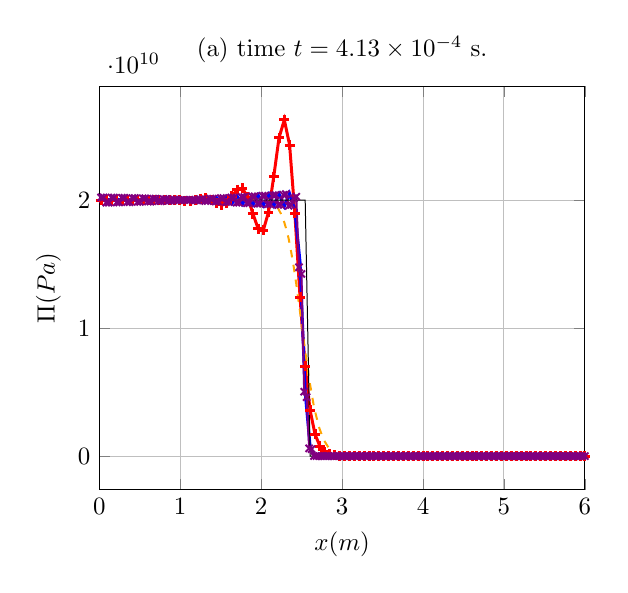
\begin{tikzpicture}[scale=0.9]
\begin{axis}[xlabel=$x (m)$,ylabel=$\Pi (Pa)$,ymajorgrids=true,xmajorgrids=true,legend pos= south west,title={(a) time $t = 4.13\times 10^{-4} $ s.},xmin=0.,xmax=6.]
\addplot[Red,very thick,mark=+,solid] coordinates {(-0.16829522461060809,20007169511.96314) (-0.10369101528636954,19993538918.151154) (-0.03910008978943477,20005752249.60066) (0.025484632606506585,19995780538.002594) (0.09006724602086946,20002982078.92515) (0.1546485608680076,19999277260.36865) (0.2192288029837782,20000480398.382977) (0.2838085169531259,20001789392.278667) (0.3483874448371409,19997301874.53342) (0.41296605184651003,20003008206.491848) (0.4775444471393354,19998613234.28465) (0.5421228879757068,20006614615.093975) (0.6067010779765869,19998205526.77761) (0.6712784021529404,19998711631.528248) (0.7358550513644272,19992106494.35627) (0.8004321132591515,20004770592.319847) (0.8650111473999984,20015779987.73382) (0.9295914037752241,20019625431.191498) (0.9941696099372187,19992929208.032467) (1.0587424231017257,19958300876.966587) (1.123311926789651,19955346446.406406) (1.1878866648233635,20018511640.579197) (1.2524750200748365,20111607980.21578) (1.3170736594252148,20136508388.211338) (1.381663458854595,20010138904.573597) (1.4462219802801475,19778030212.99804) (1.5107477640922773,19635427268.59183) (1.5752752811607438,19797599632.74197) (1.639859880303798,20289327749.506416) (1.70453378203858,20824737676.284462) (1.769262079187512,20916782028.057846) (1.8339384337847504,20225825740.178158) (1.89844144581174,18932646585.446335) (1.9627281077084087,17775081852.48631) (2.026899949421701,17642004813.115726) (2.091185400436795,19055892736.768036) (2.1558364961562164,21827268031.841457) (2.220982442003199,24860462590.307526) (2.286498524038505,26265768115.97021) (2.351967307290947,24295998059.88075) (2.4168137711136564,18956883378.505733) (2.480598163334301,12418144526.81467) (2.543246483139721,7028504053.174823) (2.604999975767945,3579770240.6871147) (2.66618758468537,1694104579.470104) (2.7270670263127124,758612765.168792) (2.7877944080472954,324010645.8165056) (2.848451732493268,132301231.12326287) (2.90907847951511,51629746.688618675) (2.969692513364221,19230481.215198454) (3.0303015063501104,6825460.685392445) (3.0909085945578147,2304741.6481061573) (3.151514997773176,739250.3468689044) (3.212121166898583,224906.37010029136) (3.2727272601131854,64808.36407273517) (3.3333333300016945,17662.648147483887) (3.3939393931074338,4546.039630207806) (3.4545454543493492,1103.2785027445323) (3.5151515151079566,252.0479295361392) (3.5757575757484754,54.104532819766206) (3.6363636363618523,10.890886483248497) (3.69696969696937,2.0511541183492015) (3.7575757575757014,0.36048087591867584) (3.81818181818181,0.05894430243048331) (3.8787878787878776,0.008907404728338756) (3.9393939393939394,0.0011956247957501686) (4.0,0.00011956247957501687) (4.0606060606060606,0.0) (4.121212121212121,0.0) (4.181818181818182,0.0) (4.242424242424242,0.0) (4.303030303030303,0.0) (4.363636363636363,0.0) (4.424242424242425,0.0) (4.484848484848485,0.0) (4.545454545454546,0.0) (4.606060606060606,0.0) (4.666666666666667,0.0) (4.7272727272727275,0.0) (4.787878787878788,0.0) (4.848484848484849,0.0) (4.909090909090909,0.0) (4.96969696969697,0.0) (5.03030303030303,0.0) (5.090909090909091,0.0) (5.151515151515151,0.0) (5.212121212121212,0.0) (5.2727272727272725,0.0) (5.333333333333334,0.0) (5.3939393939393945,0.0) (5.454545454545455,0.0) (5.515151515151516,0.0) (5.575757575757576,0.0) (5.636363636363637,0.0) (5.696969696969697,0.0) (5.757575757575758,0.0) (5.818181818181818,0.0) (5.878787878787879,0.0) (5.9393939393939394,0.0) (6.0,0.0) };
\addplot[Blue,very thick,mark=none,solid] coordinates {(-0.17172662820924992,20126286105.84016) (-0.10660603391933107,19875164406.999718) (-0.04194663943234102,20122512972.128735) (0.022732395165806486,19881553883.263596) (0.08741156754331267,20113695600.0826) (0.15209029604815277,19892923663.406227) (0.21677157984023532,20099953165.28105) (0.2814513737028933,19909115868.450443) (0.3461348221041776,20081472085.12577) (0.4108152742186133,19929906305.25904) (0.4755009353032759,20058503290.3213) (0.5401815288947392,19955007831.504406) (0.6048694507202782,20031358457.677605) (0.6695495822549338,19984074913.32308) (0.7342398618126412,20000405141.87171) (0.7989189035565396,20016709438.584362) (0.8636117080664685,19966060744.260063) (0.9282890378442423,20052467818.751507) (0.9929846146963595,19928785275.12034) (1.0576596352554701,20090869363.82577) (1.1223583072987158,19889072904.409824) (1.1870304528999478,20131405850.072147) (1.2517326020503938,19847442355.372017) (1.3164013359003341,20173552123.78648) (1.3811073800322917,19804426272.137638) (1.4457721874723826,20216777502.470745) (1.5104825561512225,19760559789.583214) (1.575142938446335,20260557805.032604) (1.6398580523466464,19716368448.944717) (1.7045135246263603,20304386827.323605) (1.769233781555915,19672356602.402267) (1.833883876574903,20347788289.080315) (1.8986096450055439,19628995435.82482) (1.96325392193934,20390327196.219734) (2.0279855406761045,19586711664.247425) (2.0926235965346587,20431618631.24346) (2.1573613774425398,19545878506.256725) (2.2219928581092483,20471336442.532116) (2.286737089006318,19506806138.044117) (2.3513616964415003,20505909410.75548) (2.416111827679838,19223361070.797165) (2.4806716443202474,15164119638.328646) (2.544309845123544,4962759374.283854) (2.605921117305293,685282540.4186183) (2.666666666666667,0.0) (2.7272727272727275,0.0) (2.787878787878788,0.0) (2.8484848484848486,0.0) (2.909090909090909,0.0) (2.9696969696969697,0.0) (3.0303030303030303,0.0) (3.090909090909091,0.0) (3.1515151515151514,0.0) (3.2121212121212124,0.0) (3.272727272727273,0.0) (3.3333333333333335,0.0) (3.393939393939394,0.0) (3.4545454545454546,0.0) (3.515151515151515,0.0) (3.5757575757575757,0.0) (3.6363636363636367,0.0) (3.6969696969696972,0.0) (3.757575757575758,0.0) (3.8181818181818183,0.0) (3.878787878787879,0.0) (3.9393939393939394,0.0) (4.0,0.0) (4.0606060606060606,0.0) (4.121212121212121,0.0) (4.181818181818182,0.0) (4.242424242424242,0.0) (4.303030303030303,0.0) (4.363636363636363,0.0) (4.424242424242425,0.0) (4.484848484848485,0.0) (4.545454545454546,0.0) (4.606060606060606,0.0) (4.666666666666667,0.0) (4.7272727272727275,0.0) (4.787878787878788,0.0) (4.848484848484849,0.0) (4.909090909090909,0.0) (4.96969696969697,0.0) (5.03030303030303,0.0) (5.090909090909091,0.0) (5.151515151515151,0.0) (5.212121212121212,0.0) (5.2727272727272725,0.0) (5.333333333333334,0.0) (5.3939393939393945,0.0) (5.454545454545455,0.0) (5.515151515151516,0.0) (5.575757575757576,0.0) (5.636363636363637,0.0) (5.696969696969697,0.0) (5.757575757575758,0.0) (5.818181818181818,0.0) (5.878787878787879,0.0) (5.9393939393939394,0.0) (6.0,0.0) };
\addplot[Orange,thick,mark=none,dashed] coordinates {(-0.17065948135616368,20000043525.826946) (-0.13846405161119207,20000131357.192825) (-0.10615855337338398,20000218494.583206) (-0.07404331926680283,20000306501.181454) (-0.04177810548697509,20000393896.47217) (-0.009673436417956368,20000482254.930782) (0.022584758948793797,20000570082.4036) (0.05468914251045678,20000658972.299118) (0.08694578874198917,20000747409.83799) (0.11905093160937343,20000837015.308666) (0.15130700223550114,20000926246.024586) (0.18341275190367462,20001016757.47824) (0.21566843234413013,20001106971.41286) (0.24777463690422233,20001198587.31625) (0.2800300115792282,20001289983.21988) (0.3121365750418777,20001382911.99803) (0.34439170296599453,20001475699.235306) (0.3764985602426821,20001570161.365646) (0.4087534845749329,20001664562.05299) (0.4408605892235251,20001760792.46614) (0.47311534282934564,20001857043.951477) (0.5052226603149179,20001955294.841774) (0.537477269066949,20002053652.623417) (0.5695847728293589,20002154196.745407) (0.6018392576971193,20002254937.886917) (0.63394692670971,20002358072.38815) (0.6662013049757795,20002461499.472862) (0.69830912223634,20002567550.322327) (0.730563408177844,20002673996.019188) (0.7626713598344566,20002783323.1565) (0.7949255653178342,20002893155.55905) (0.8270336401018328,20003006158.999344) (0.8592877752388308,20003119788.01011) (0.8913959639439372,20003236915.248775) (0.9236500375876889,20003354800.358326) (0.9557583325989031,20003476555.48888) (0.988012352597941,20003599215.36085) (1.0201207475700413,20003726170.38179) (1.0523747209384142,20003854194.74781) (1.0844832106025044,20003987003.679684) (1.1167371437039924,20004121068.23257) (1.1488457237196221,20004260484.92572) (1.1810996224233543,20004401370.18105) (1.2132082892569704,20004548271.07166) (1.2454621590450947,20004696886.54289) (1.2775709098908066,20004852300.090237) (1.309824755958588,20005009715.66264) (1.3419335886911143,20005174860.54694) (1.3741874160526513,20005342346.906036) (1.4062963291967852,20005518680.70837) (1.4385501427858645,20005697758.81623) (1.4706591355042127,20005887046.311424) (1.5029129402719827,20006079555.280518) (1.5350220123805445,20006284041.2585) (1.5672758134024902,20006492358.140556) (1.5993849654540777,20006715414.269215) (1.631638768111729,20006943437.753944) (1.6637480016793325,20007191089.639084) (1.6960018121418028,20007446834.098385) (1.7281111303121328,20007725459.210213) (1.7603649564409494,20008019319.813942) (1.7924743621157493,20008294004.40781) (1.824728211751267,20008585840.13172) (1.8568376886603435,20008554541.09674) (1.8890915456370228,20008462505.522263) (1.9212009637009544,20006730940.889435) (1.9534546670018174,20004485622.310314) (1.9855634459187166,19996264844.062057) (2.0178162660757217,19985866912.241154) (2.049922432994727,19957886954.48237) (2.0821719106575194,19923019878.742535) (2.1142699487559726,19844752482.056076) (2.146509305404184,19748673138.130287) (2.1785861511174294,19561739730.699345) (2.210799592712115,19335939752.423916) (2.24282884289106,18950316261.230713) (2.2749849883928817,18492945635.84119) (2.3069214957996795,17806784492.6505) (2.338967747836579,17010629044.48117) (2.3707479648286887,15966022841.692478) (2.4026123302922753,14785812065.51804) (2.434166526992342,13436743410.941061) (2.4657735751955867,11958066788.981596) (2.497049074903414,10483331170.150602) (2.528347122496258,8916511769.703724) (2.5593295703130683,7540569940.703419) (2.590312212342123,6120676372.669546) (2.6210295241339954,5005409973.170741) (2.651735403923134,3883807857.160711) (2.6822429663855347,3081223065.2520843) (2.712736226853065,2292253118.873356) (2.7430959078472834,1769087143.9346516) (2.773443251962098,1265410542.8025982) (2.803708355333792,951803900.811647) (2.8339646430982732,655843903.0110523) (2.864174119091245,481283905.106187) (2.894378051323549,319756521.6427987) (2.924557159507066,229045727.21750608) (2.954733115412435,146743624.4075898) (2.984896753012443,102624770.99267791) (3.015058747688463,63378554.38021657) (3.0452150104299562,43277421.13854273) (3.075370482653709,25746439.23638048) (3.105523452064602,17166812.660074137) (3.1356760689168683,9830289.851074612) (3.1658276603124804,6400759.483536921) (3.195979105635568,3525021.159262417) (3.226130156857271,2241699.5574820205) (3.2562811517774475,1186278.3528258102) (3.2864320046978017,736934.7477214294) (3.3165828374132054,374402.79637388245) (3.346733622184799,227248.07808513625) (3.3768844002016,110745.8468615504) (3.4070351630577127,65691.86429748994) (3.4371859238094924,30680.492705236302) (3.467336680073573,17790.289802416904) (3.497487435726684,7955.149116569932) (3.5276381901369445,4510.511505733829) (3.55778894438189,1929.1940661950573) (3.587939698304978,1069.8799239515781) (3.6180904521863875,437.2341897356511) (3.6482412059899048,237.23724715030917) (3.6783919597836334,92.53448438029154) (3.7085427135597566,49.13748895850961) (3.73869346733374,18.270581630057357) (3.7688442211040107,9.498103159014207) (3.7989949748738456,3.3623360506506152) (3.82914572864295,1.711835801326188) (3.859296482411972,0.5762313703130271) (3.8894472361808607,0.28742820089864735) (3.9195979899497346,0.09200332803300691) (3.9497487437185868,0.0450750547997889) (3.9798994974874353,0.013749685151127641) (4.01005025125628,0.006635717616413599) (4.040201005025126,0.0019727809129877925) (4.0703517587939695,0.0008967185968126294) (4.100502512562814,0.0003586874387250511) (4.130653266331658,0.00011956247957501691) (4.160804020100502,0.0) (4.190954773869347,0.0) (4.221105527638191,0.0) (4.251256281407035,0.0) (4.281407035175879,0.0) (4.311557788944723,0.0) (4.341708542713568,0.0) (4.371859296482412,-5.9781239787508415e-05) (4.402010050251256,0.0) (4.4321608040201,0.0) (4.4623115577889445,0.0) (4.492462311557789,0.0) (4.522613065326633,0.0) (4.552763819095477,0.0) (4.582914572864321,0.0) (4.613065326633166,0.0) (4.64321608040201,0.0) (4.673366834170854,-5.9781239787508415e-05) (4.703517587939698,0.0) (4.733668341708542,-5.9781239787508415e-05) (4.763819095477387,0.0) (4.793969849246231,0.0) (4.824120603015075,0.0) (4.8542713567839195,0.0) (4.884422110552763,0.0) (4.914572864321608,0.0) (4.944723618090452,0.0) (4.974874371859296,-5.9781239787508415e-05) (5.005025125628141,0.0) (5.035175879396984,-5.9781239787508415e-05) (5.065326633165829,0.0) (5.0954773869346734,0.0) (5.125628140703517,0.0) (5.155778894472362,0.0) (5.185929648241205,0.0) (5.21608040201005,0.0) (5.2462311557788945,0.0) (5.276381909547738,-5.9781239787508415e-05) (5.306532663316583,0.0) (5.3366834170854265,-5.9781239787508415e-05) (5.366834170854271,0.0) (5.396984924623116,0.0) (5.427135678391959,0.0) (5.457286432160804,0.0) (5.487437185929648,0.0) (5.517587939698492,0.0) (5.547738693467337,0.0) (5.57788944723618,-5.9781239787508415e-05) (5.608040201005025,0.0) (5.638190954773869,-5.9781239787508415e-05) (5.668341708542713,0.0) (5.698492462311558,0.0) (5.7286432160804015,0.0) (5.758793969849246,0.0) (5.788944723618091,0.0) (5.819095477386934,0.0) (5.849246231155779,5.978123978750844e-05) (5.879396984924623,-5.9781239787508415e-05) (5.909547738693467,0.0) (5.939698492462312,0.0) (5.969849246231155,0.0) (6.0,0.0) };
\addplot[Purple,thick,mark=x,solid] coordinates {(-0.1708904472675148,19785557608.354362) (-0.141053536291792,19785867406.07991) (-0.10639968665550317,20213101585.682953) (-0.07596722729975139,20213166639.459328) (-0.04207388662674958,19789540452.376034) (-0.011506607675021027,19789557029.70826) (0.022285105176351794,20207044209.230186) (0.052869007707743255,20207022244.274338) (0.08665834628959812,19798347997.174698) (0.1172321822636404,19798342777.723587) (0.151029412846739,20196099111.801785) (0.18158911289003257,20196061786.86517) (0.2154029118177921,19812014870.030228) (0.24594855907990398,19812000299.62603) (0.2797707639479692,20180456497.651028) (0.31030435509337834,20180413575.280464) (0.34414190966292796,19830391975.858875) (0.3746654464197197,19830363703.36432) (0.4085073802039732,20160337163.972836) (0.4390230930475627,20160297191.04402) (0.4728761360608775,19853261920.69269) (0.5033851748227214,19853214144.348965) (0.5372398018663066,20136017953.04032) (0.5677435687389828,20135992244.21921) (0.6016065301582988,19880348866.887726) (0.6321057005127878,19880275931.784782) (0.6659696058844139,20107829473.983624) (0.696465113347797,20107832721.84703) (0.7303345889699686,19911323145.714508) (0.7608267981523694,19911220393.101494) (0.794698155191189,20076150936.708942) (0.8251876402029276,20076201595.577923) (0.8590614435557611,19945806771.791153) (0.8895483774038433,19945671337.662453) (0.9234264348463641,20041403461.894547) (0.9539111397029185,20041524039.151882) (0.9877878427021151,19983380229.063835) (1.0182704154578464,19983211779.396458) (1.0521550389906216,20004041901.242966) (1.0826356465144116,20004259130.529278) (1.1165141722198928,20023590444.9662) (1.146992928994242,20023391823.879498) (1.1808842235337922,19964545222.656155) (1.2113612103069733,19964890116.037624) (1.2452405366181794,20065959588.155254) (1.2757159448575515,20065737455.962234) (1.3096140087494017,19923405655.590446) (1.340087867199397,19923913531.19163) (1.3739668745812406,20109993427.265583) (1.4044394740876944,20109759370.691113) (1.4383442989671855,19881117133.925976) (1.4688156172979114,19881828092.426723) (1.5026930749798657,20155184504.96013) (1.5331634940260768,20154958787.012196) (1.5670749872969294,19838167967.197243) (1.5975444109704615,19839129929.862263) (1.631419066113116,20201034036.189003) (1.6618879405221585,20200860914.39588) (1.695806028986006,19795048344.53005) (1.7262741487880973,19796331467.05578) (1.7601448712991692,20247083731.9241) (1.7906127153916045,20247094549.42775) (1.8245374872621891,19752175452.996067) (1.8550046971339533,19753935406.555477) (1.888870629478351,20292760865.435543) (1.9193376913168196,20293432983.43762) (1.953269542435462,19709654117.014126) (1.9837358641666532,19712407968.009735) (2.0175965864610483,20337138548.75029) (2.048062639992706,20340344997.290543) (2.082002580382462,19666867314.68073) (2.1124672812076257,19672700955.769726) (2.1463232982512577,20378078322.74046) (2.1767870343556104,20391295863.689228) (2.210737854430747,19619814494.093407) (2.241198117559328,19637708700.528072) (2.275052752024238,20408768422.209846) (2.3055096404249302,20461791611.02041) (2.339480401341693,19548900704.7548) (2.3699263513980036,19618213930.10675) (2.4037921787393377,20126713795.32762) (2.4342241255841532,20264753853.55581) (2.468186972434222,14751152292.966133) (2.4985606945703163,14228242465.12349) (2.531508975979028,5032326878.965216) (2.5617596336243342,4603536576.276086) (2.592841768880457,605310239.9535259) (2.623005846412341,539574226.1837834) (2.6532663316582914,0.0005380311580875769) (2.6834170854271355,0.0005380311580875769) (2.7135678391959797,0.0005380311580875769) (2.743718592964824,0.0004782499183000683) (2.7738693467336684,0.0005978123978750856) (2.8040201005025125,0.0005978123978750856) (2.8341708542713566,0.0005380311580875769) (2.8643216080402008,0.0005380311580875769) (2.8944723618090453,0.0005978123978750856) (2.9246231155778895,0.0005978123978750856) (2.9547738693467336,0.0004184686785125597) (2.9849246231155777,0.0003586874387250511) (3.015075376884422,0.0004782499183000683) (3.0452261306532664,0.0004184686785125597) (3.0753768844221105,0.0003586874387250511) (3.1055276381909547,0.0003586874387250511) (3.135678391959799,0.0005380311580875769) (3.165829145728643,0.0005380311580875769) (3.1959798994974875,0.0004184686785125597) (3.2261306532663316,0.0004184686785125597) (3.2562814070351758,0.0004782499183000683) (3.28643216080402,0.0004184686785125597) (3.316582914572864,0.0004782499183000683) (3.3467336683417086,0.0004184686785125597) (3.3768844221105527,0.0004184686785125597) (3.407035175879397,0.0003586874387250511) (3.437185929648241,0.0003586874387250511) (3.467336683417085,0.0003586874387250511) (3.4974874371859297,0.0003586874387250511) (3.527638190954774,0.0003586874387250511) (3.557788944723618,0.0003586874387250511) (3.587939698492462,0.0003586874387250511) (3.618090452261306,0.0003586874387250511) (3.648241206030151,0.0003586874387250511) (3.678391959798995,0.0002989061989375425) (3.708542713567839,0.0002989061989375425) (3.738693467336683,0.0004184686785125597) (3.7688442211055273,0.0004184686785125597) (3.798994974874372,0.0003586874387250511) (3.829145728643216,0.0003586874387250511) (3.85929648241206,0.0001793437193625254) (3.8894472361809043,0.0001793437193625254) (3.9195979899497484,0.0001793437193625254) (3.949748743718593,0.00011956247957501691) (3.979899497487437,0.0003586874387250511) (4.010050251256281,0.0002989061989375425) (4.040201005025126,0.0002989061989375425) (4.0703517587939695,0.0002989061989375425) (4.100502512562814,0.00023912495915003393) (4.130653266331658,0.0003586874387250511) (4.160804020100502,0.0003586874387250511) (4.190954773869347,0.0003586874387250511) (4.221105527638191,0.0003586874387250511) (4.251256281407035,0.0003586874387250511) (4.281407035175879,0.0003586874387250511) (4.311557788944723,0.0003586874387250511) (4.341708542713568,0.0002989061989375425) (4.371859296482412,0.0002989061989375425) (4.402010050251256,0.00023912495915003393) (4.4321608040201,0.00023912495915003393) (4.4623115577889445,0.00023912495915003393) (4.492462311557789,0.00023912495915003393) (4.522613065326633,0.0002989061989375425) (4.552763819095477,0.0002989061989375425) (4.582914572864321,0.0002989061989375425) (4.613065326633166,0.00023912495915003393) (4.64321608040201,0.0003586874387250511) (4.673366834170854,0.0003586874387250511) (4.703517587939698,0.0002989061989375425) (4.733668341708542,0.00023912495915003393) (4.763819095477387,0.0002989061989375425) (4.793969849246231,0.0002989061989375425) (4.824120603015075,0.0002989061989375425) (4.8542713567839195,0.0002989061989375425) (4.884422110552763,0.0003586874387250511) (4.914572864321608,0.0003586874387250511) (4.944723618090452,0.00023912495915003393) (4.974874371859296,0.00023912495915003393) (5.005025125628141,0.0003586874387250511) (5.035175879396984,0.0002989061989375425) (5.065326633165829,0.0002989061989375425) (5.0954773869346734,0.0002989061989375425) (5.125628140703517,0.00023912495915003393) (5.155778894472362,0.0002989061989375425) (5.185929648241205,0.0003586874387250511) (5.21608040201005,0.0003586874387250511) (5.2462311557788945,0.0001793437193625254) (5.276381909547738,0.0001793437193625254) (5.306532663316583,0.0002989061989375425) (5.3366834170854265,0.00023912495915003393) (5.366834170854271,0.00023912495915003393) (5.396984924623116,0.00023912495915003393) (5.427135678391959,0.00023912495915003393) (5.457286432160804,0.00023912495915003393) (5.487437185929648,0.0001793437193625254) (5.517587939698492,0.00011956247957501691) (5.547738693467337,5.978123978750844e-05) (5.57788944723618,5.978123978750844e-05) (5.608040201005025,0.0001793437193625254) (5.638190954773869,0.0001793437193625254) (5.668341708542713,0.00023912495915003393) (5.698492462311558,0.0001793437193625254) (5.7286432160804015,0.00011956247957501691) (5.758793969849246,5.978123978750844e-05) (5.788944723618091,0.00011956247957501691) (5.819095477386934,5.978123978750844e-05) (5.849246231155779,0.0) (5.879396984924623,0.0) (5.909547738693467,0.0) (5.939698492462312,5.978123978750844e-05) (5.969849246231155,-0.0001195624795750168) (6.0,0.0) };
\addplot[black,thin,mark=none,solid] coordinates {(-0.17172662820924992,19999999999.999966) (-0.10660603391933107,19999999999.999966) (-0.04194663943234102,19999999999.999966) (0.022732395165806486,19999999999.999966) (0.08741156754331267,19999999999.999966) (0.15209029604815277,19999999999.999966) (0.21677157984023532,19999999999.999966) (0.2814513737028933,19999999999.999966) (0.3461348221041776,19999999999.999966) (0.4108152742186133,19999999999.999966) (0.4755009353032759,19999999999.999966) (0.5401815288947392,19999999999.999966) (0.6048694507202782,19999999999.999966) (0.6695495822549338,19999999999.999966) (0.7342398618126412,19999999999.999966) (0.7989189035565396,19999999999.999966) (0.8636117080664685,19999999999.999966) (0.9282890378442423,19999999999.999966) (0.9929846146963595,19999999999.999966) (1.0576596352554701,19999999999.999966) (1.1223583072987158,19999999999.999966) (1.1870304528999478,19999999999.999966) (1.2517326020503938,19999999999.999966) (1.3164013359003341,19999999999.999966) (1.3811073800322917,19999999999.999966) (1.4457721874723826,19999999999.999966) (1.5104825561512225,19999999999.999966) (1.575142938446335,19999999999.999966) (1.6398580523466464,19999999999.999966) (1.7045135246263603,19999999999.999966) (1.769233781555915,19999999999.999966) (1.833883876574903,19999999999.999966) (1.8986096450055439,19999999999.999966) (1.96325392193934,19999999999.999966) (2.0279855406761045,19999999999.999966) (2.0926235965346587,19999999999.999966) (2.1573613774425398,19999999999.999966) (2.2219928581092483,19999999999.999966) (2.286737089006318,19999999999.999966) (2.3513616964415003,19999999999.999966) (2.416111827679838,19999999999.999966) (2.4806716443202474,19999999999.999966) (2.544309845123544,19999999999.999966) (2.605921117305293,0.0) (2.666666666666667,0.0) (2.7272727272727275,0.0) (2.787878787878788,0.0) (2.8484848484848486,0.0) (2.909090909090909,0.0) (2.9696969696969697,0.0) (3.0303030303030303,0.0) (3.090909090909091,0.0) (3.1515151515151514,0.0) (3.2121212121212124,0.0) (3.272727272727273,0.0) (3.3333333333333335,0.0) (3.393939393939394,0.0) (3.4545454545454546,0.0) (3.515151515151515,0.0) (3.5757575757575757,0.0) (3.6363636363636367,0.0) (3.6969696969696972,0.0) (3.757575757575758,0.0) (3.8181818181818183,0.0) (3.878787878787879,0.0) (3.9393939393939394,0.0) (4.0,0.0) (4.0606060606060606,0.0) (4.121212121212121,0.0) (4.181818181818182,0.0) (4.242424242424242,0.0) (4.303030303030303,0.0) (4.363636363636363,0.0) (4.424242424242425,0.0) (4.484848484848485,0.0) (4.545454545454546,0.0) (4.606060606060606,0.0) (4.666666666666667,0.0) (4.7272727272727275,0.0) (4.787878787878788,0.0) (4.848484848484849,0.0) (4.909090909090909,0.0) (4.96969696969697,0.0) (5.03030303030303,0.0) (5.090909090909091,0.0) (5.151515151515151,0.0) (5.212121212121212,0.0) (5.2727272727272725,0.0) (5.333333333333334,0.0) (5.3939393939393945,0.0) (5.454545454545455,0.0) (5.515151515151516,0.0) (5.575757575757576,0.0) (5.636363636363637,0.0) (5.696969696969697,0.0) (5.757575757575758,0.0) (5.818181818181818,0.0) (5.878787878787879,0.0) (5.9393939393939394,0.0) (6.0,0.0) };
%\legend{mpm,dgmpm,dgmpm 2ppc,dgmpm 2ppc (RK2),exact}
\end{axis}
\end{tikzpicture}
%%% Local Variables:
%%% mode: latex
%%% TeX-master: "../../mainManuscript"
%%% End:
}
  {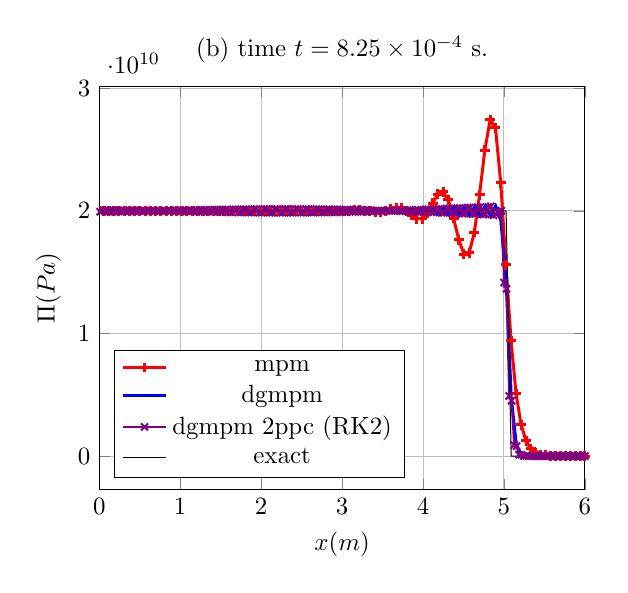
\begin{tikzpicture}[scale=0.9]
\begin{axis}[xlabel=$x (m)$,ylabel=$\Pi (Pa)$,ymajorgrids=true,xmajorgrids=true,legend pos= south west,title={(b) time $t = 8.25\times 10^{-4} $ s.},xmin=0.,xmax=6.]
\addplot[Red,very thick,mark=+,solid] coordinates {(-0.3373970335129395,20002444911.789238) (-0.2727928966297102,19997432693.913857) (-0.20820196231046736,20001959247.078884) (-0.14361740752040095,19997652072.059658) (-0.0790347885190633,20001174478.201954) (-0.014453732919982308,19998113117.396988) (0.050126384917715185,20000219977.304207) (0.1147058039394095,19998668866.378258) (0.17928462960154493,19999250601.410038) (0.24386307172432597,19999169326.347557) (0.30844111377254735,19998402881.7715) (0.3730189157030712,19999501047.64978) (0.43759644654074153,19997762967.548557) (0.50217381047918,19999609942.781967) (0.5667509959420945,19997354773.840668) (0.6313280560675543,19999501477.373802) (0.6959050053014575,19997148374.83382) (0.7604818569685504,19999225474.73323) (0.8250586461934166,19997083680.145477) (0.8896353603808954,19998851023.15548) (0.9542120453300287,19997089910.935226) (1.0187886757648426,19998440828.306694) (1.083365299089184,19997111161.46065) (1.1479418881286723,19998051169.644836) (1.2125184850646817,19997116278.583233) (1.2770950657270574,19997699692.89216) (1.3416716627444705,19997067231.472904) (1.406248258920999,19997388896.74777) (1.4708248806644153,19997000578.277737) (1.535401519422826,19997171020.844025) (1.599978191235337,19996918101.970993) (1.6645548853210443,19996920744.490818) (1.7291316080867047,19996700814.432293) (1.7937083617143608,19996691407.553604) (1.8582851678967984,19996686120.493286) (1.9228620377138623,19996772465.623905) (1.9874389634593603,19996650100.204838) (2.0520159097351134,19996304228.832874) (2.1165928542213344,19995901639.208565) (2.181169830867098,19995922422.124294) (2.245746933014004,19996569013.601753) (2.3103242301117346,19997366737.300365) (2.3749016574282744,19997253707.766594) (2.439479003437918,19995610575.776176) (2.50405608348629,19993366031.355854) (2.5686330012527394,19992897527.09602) (2.633210227393201,19996035016.03268) (2.6977882771955914,20001461417.7394) (2.7623671197745874,20004234447.067886) (2.826945847657703,19999248815.338493) (2.891523147056034,19986954084.876858) (2.9560985175931442,19976226893.658413) (3.020673338478683,19979732556.833313) (3.0852505531422554,20002734650.377262) (3.149832540815079,20033514677.442947) (3.2144183646554727,20045779859.54768) (3.279002790793957,20016543982.692215) (3.343578922732655,19949761640.288918) (3.408143766461,19886271903.166637) (3.472703046370895,19885090545.547707) (3.5372706584700393,19980762153.863453) (3.6018608542803987,20143069670.253544) (3.666476517033703,20272160418.98628) (3.731101311045297,20247014960.951336) (3.7957034722589915,20011400843.260548) (3.8602530814356824,19644164431.403908) (3.924745093767238,19352701051.419342) (3.9892134274545104,19373330976.866657) (4.0537234224180505,19827324507.865147) (4.118341053895788,20606668355.762043) (4.183090744717796,21350802856.75598) (4.247923050028822,21564506017.293846) (4.312715450250743,20887275093.29332) (4.37731903294961,19390073952.106243) (4.441637416097922,17648045449.929543) (4.505695564266106,16477972514.036726) (4.569656065119688,16564993555.823458) (4.633774257438693,18234485218.06143) (4.698311215790016,21316982189.19614) (4.763422276660747,24943663529.441895) (4.829040675663493,27423065710.3382) (4.894809718237837,26786511205.121754) (4.960153433745974,22304704037.851227) (5.024529459659876,15612866271.729282) (5.0877165905602455,9395941456.960642) (5.149868001086729,5080803829.979227) (5.211310703936358,2571948063.5769763) (5.2723407989116975,1251943821.049851) (5.333153160181875,594362859.6955562) (5.393856948062081,276921639.57925117) (5.454508383498881,126868092.89648758) (5.515135140653742,57148823.407327816) (5.575750476779182,25288021.07216049) (5.636360618733436,10978518.189306797) (5.696968440582231,4670443.034755671) (5.757575245750145,1944881.6231991085) (5.818181614449599,792440.4555923982) (5.878787799930788,317032.1081128554) (5.939393910671728,128397.83825474144) (5.9999999928647405,63394.068050559574) };
\addplot[Blue,very thick,mark=none,solid] coordinates {(-0.34300326824190164,19867161670.92257) (-0.27788319029024855,20132353190.445465) (-0.21322278871058642,19869130721.386837) (-0.14854524891661086,20129142425.138195) (-0.08386416618006085,19873652842.561867) (-0.01918775421833607,20123421266.062355) (0.04549613686190245,19880628150.922165) (0.11017305016981589,20115318727.80989) (0.17485949985090674,19889901681.750263) (0.2395368602373047,20105017064.568512) (0.30422552430806427,19901266649.63073) (0.36890325481559005,20092747885.067688) (0.43359370903377453,19914468812.52206) (0.4982717227365738,20078787280.255478) (0.5629635229582883,19929211827.51738) (0.6276417735241854,20063450128.705578) (0.6923344895943412,19945162699.15721) (0.7570129870707453,20047081201.542427) (0.8217062271247281,19961961586.06754) (0.8863850430702915,20030053095.45937) (0.9510784635094146,19979226355.574352) (1.015757722065038,20012756186.25665) (1.0804510262905567,19996560201.361286) (1.1451308857252085,19995591078.27326) (1.2098238162869241,20013559902.98507) (1.2745044463948634,19978961181.23721) (1.339196775641803,20029823630.182865) (1.40387833619713,19963265075.256836) (1.468569859873193,20044958518.655983) (1.533252484114899,19948889080.898514) (1.5979430206134242,20058587899.768158) (1.6626268056632443,19936200167.451828) (1.7273162014193637,20070358058.719982) (1.7920012052713876,19925539314.253044) (1.8566893446755617,20079944419.1636) (1.9213755875853589,19917215422.042995) (1.9860624044406507,20087057076.01931) (2.0507498716789403,19911499852.8977) (2.115435358948472,20091445622.53556) (2.1801240021419153,19908621665.315594) (2.244808217516759,20092903240.062386) (2.3094979529589694,19908763592.066013) (2.3741810192336423,20091270026.991108) (2.4388717231008803,19912058799.92498) (2.503553823894505,20086435560.409016) (2.568245325654722,19918588470.128216) (2.6329266981213357,20078340688.316597) (2.6976187741402335,19928380238.783928) (2.762299700805929,20066978548.729008) (2.826992075723227,19941407541.779408) (2.891672923066381,20052394804.467094) (2.956365346939235,19957589915.641735) (3.0210465161215225,20034687069.70895) (3.0857385707248404,19976794311.40647) (3.150420408966768,20014003488.348423) (3.2151116547381915,19998837479.325516) (3.279794587709358,19990540408.2874) (3.3444845724109693,20023489474.801964) (3.4091690555988876,19964539084.58109) (3.4738573026283968,20050478317.273846) (3.5385438113443364,19936281343.307373) (3.6032298274016155,20079495802.060196) (3.667918848609329,19906084152.544304) (3.732602130509684,20110204420.136734) (3.7972941529817468,19874293081.001152) (3.8619741937006657,20142245283.97256) (3.926669697644514,19841274680.052853) (3.9913459924348733,20175246892.79887) (4.056045440000399,19807407898.849144) (4.120717493458492,20208834504.42018) (4.185421321345374,19773074740.97144) (4.250088655916392,20242639943.665905) (4.314797270727306,19738650272.25273) (4.379459436438253,20276310806.877926) (4.44417321250515,19704493074.44567) (4.508829797148642,20309519959.73904) (4.573549076088961,19670935330.734615) (4.638199714390607,20341974420.673492) (4.702924805180256,19638273500.285717) (4.767569185544008,20373421858.440434) (4.832300363715842,19606757017.834343) (4.896938230755509,20398348853.4957) (4.961674477599282,19194568925.629593) (5.026219132132484,14312041520.443619) (5.089697845458756,4819432981.92643) (5.151288275508455,961012171.3536986) (5.212092547900456,129265691.8128923) (5.272725221999611,10032930.422299773) (5.333333333333334,0.0) (5.3939393939393945,0.0) (5.454545454545455,0.0) (5.515151515151516,0.0) (5.575757575757576,0.0) (5.636363636363637,0.0) (5.696969696969697,0.0) (5.757575757575758,0.0) (5.818181818181818,0.0) (5.878787878787879,0.0) (5.9393939393939394,0.0) (6.0,0.0) };
\addplot[Purple,thick,mark=x,solid] coordinates {(-0.3413421216005564,20084454120.70626) (-0.3115046323967783,20084503231.20538) (-0.2768503231825786,19916185104.896652) (-0.24641699137696205,19916224025.277943) (-0.21252704225382044,20082521029.067745) (-0.18195851890502224,20082494630.53035) (-0.14816447224841806,19919503737.228157) (-0.11757957066435366,19919560593.514977) (-0.08379589265784985,20077952554.12534) (-0.05322085703338879,20077898893.370735) (-0.019419148715127472,19925390458.555717) (0.011141460181846741,19925475541.195904) (0.04494772591031657,20070870972.704773) (0.07549443808768144,20070794153.22469) (0.10932301412763686,19933726420.88046) (0.13985737952332528,19933837024.581604) (0.173685926639547,20061431321.92105) (0.20421035859246994,20061332816.082695) (0.23806014963800134,19944334708.452976) (0.2685764825007371,19944466366.306778) (0.3024195284182063,20049838277.438824) (0.33292927588669197,20049719936.704403) (0.3667927137931127,19956995564.425697) (0.39729694359154255,19957143051.16299) (0.43114948448894214,20036346157.64271) (0.4616491777370185,20036210511.364494) (0.49552220217347964,19971448924.99579) (0.5260180299294327,19971606591.563793) (0.5598772972948788,20021247143.683044) (0.5903698622131245,20021097455.275764) (0.624249900829884,19987369347.34896) (0.654739595219531,19987531478.95478) (0.6886040890282352,20004870125.83432) (0.7190912475113203,20004710463.922737) (0.7529767194177145,20004410302.615177) (0.7834615704641484,20004571380.654194) (0.8173305879064932,19987574487.067276) (0.847813305881258,19987409722.84234) (0.8817031821057704,20022200269.99343) (0.9121839339935235,20022355214.726463) (0.9460571483764127,19969742299.809765) (0.9765360354593392,19969578036.0323) (1.0104294819309994,20040348503.200268) (1.040906682974281,20040492861.37563) (1.0747838335358735,19951770413.041492) (1.105259430932844,19951612839.252544) (1.1391555845596315,20058452407.676346) (1.1696298054671987,20058582471.461685) (1.2035105315252492,19934062461.007298) (1.2339834581168863,19933918134.766502) (1.26788134906568,20076105339.2744) (1.2983532590129288,20076218192.12232) (1.332237072733504,19917020987.71109) (1.3627080375199254,19916896548.399593) (1.3966066343017862,20092904393.807842) (1.4270769595734558,20092997886.904884) (1.4609633199405618,19901039886.204426) (1.4914330391974988,19900941714.78726) (1.5253313681450775,20108457966.61612) (1.5558007815742427,20108530636.852116) (1.58968921499868,19886497320.08024) (1.620158288063799,19886431164.442165) (1.6540555703547062,20122392933.588875) (1.6845245667812516,20122443880.233562) (1.7184147802161702,19873749252.240623) (1.7488835761357309,19873719842.724926) (1.7827793345331566,20134361342.940174) (1.8132481375124534,20134390084.955162) (1.8471400866548187,19863123660.159065) (1.8776086764287256,19863134343.309586) (1.9115027873522425,20144046533.93617) (1.941971308324001,20144052872.731007) (1.9758652132489007,19854915473.262917) (2.00633335571715,19854967893.19228) (2.040226079745077,20151168618.87888) (2.070693985199334,20151152531.999393) (2.104590384682496,19849382232.053566) (2.135057901533144,19849476088.127354) (2.1689496169030114,20155489277.933567) (2.199417036193448,20155450867.5519) (2.2333157795929726,19846740444.56689) (2.263782879164934,19846873351.154137) (2.29767330438176,20156815822.998478) (2.328140263166214,20156755339.15534) (2.3620411522751077,19847162606.42877) (2.392507699460935,19847330075.36992) (2.426397066000551,20155004487.461292) (2.456863380789038,20154922439.98095) (2.4907664359543715,19850774856.538464) (2.5212322666486426,19850970415.948395) (2.555120899476285,20149962895.29097) (2.585586439450331,20149860260.53971) (2.6194915665074547,19857655259.362076) (2.649956589833981,19857870713.761578) (2.6838448104013497,20141651656.730064) (2.7143095156589245,20141530176.422417) (2.7482165060193036,19867832720.558792) (2.7786806902628784,19868058547.559307) (2.8125688393803885,20130084962.0052) (2.8430326926994947,20129947521.903427) (2.8769412584352323,19881286508.15238) (2.907404596472946,19881512377.22646) (2.9412930658856,20115330328.24148) (2.9717560576395274,20115181396.04708) (3.0056658655431305,19897946940.899014) (3.036128344041352,19898162329.4085) (3.070017595121079,20097507428.18806) (3.100479700762355,20097353520.394882) (3.1343903886946634,19917696528.872005) (3.164851976527314,19917891402.385876) (3.1987425343389657,20076785327.117977) (3.2292037151467032,20076635470.893406) (3.2631148843368862,19940372025.717415) (3.29357554543851,19940537544.133724) (3.3274679679788997,20053378728.587624) (3.357928194540636,20053244881.13022) (3.3918393831412645,19965767607.411438) (3.422299107793317,19965896815.490192) (3.456193940921393,20027543050.174908) (3.486653228633958,20027440439.6467) (3.520563880585621,19993639102.67711) (3.5510227208761473,19993727568.79394) (3.5849204556914755,19999568290.3942) (3.615378895931043,19999515651.498085) (3.649288342283673,20023709203.216496) (3.6797464349135187,20023755595.7377) (3.7136474841959903,19969771717.557053) (3.744105255467703,19969791423.13771) (3.7780127218729365,20055673406.51396) (3.8084702852479175,20055680096.82016) (3.8423749893302808,19938489456.48) (3.8728323391771236,19938607645.218704) (3.906736984687898,20089205875.665604) (3.9371942857875872,20089180050.754776) (3.971102948275359,19906067025.556553) (4.001560146502916,19906314216.038258) (4.035461128102997,20123961775.83972) (4.065918424699022,20123919131.594395) (4.099831368443375,19872848196.356743) (4.130288641421362,19873262528.891777) (4.164185191417915,20159573473.009506) (4.194642662567189,20159553030.56887) (4.228560290996899,19839166473.88708) (4.259017750563116,19839808941.31075) (4.292909258187191,20195675341.985744) (4.323366935108609,20195799856.708904) (4.357289795589992,19805336038.508987) (4.387747366655722,19806358551.373158) (4.421633460585793,20231834709.36628) (4.452091150023708,20232554202.447742) (4.48602003137047,19771483196.513275) (4.516477347673006,19773429826.418495) (4.5503580637774,20267126470.97277) (4.58081526693636,20270193617.440983) (4.614751454576072,19736918846.87252) (4.645207821787056,19742059913.02803) (4.679083775444953,20298852761.491997) (4.7095395048223025,20311197166.66586) (4.743485099523246,19697906198.47693) (4.773938201390833,19716155926.428547) (4.807812253028679,20317459432.2131) (4.838261988618075,20366464115.49615) (4.872224665961511,19636335499.984386) (4.9026646932738345,19711246044.137264) (4.936550533899874,19912517877.28153) (4.966975247749498,20015432325.29268) (5.000903022698816,14157492462.311962) (5.031270011791101,13637448020.679394) (5.064107380705877,4900151134.711801) (5.094355634519364,4518545375.67135) (5.125418372928627,896010785.5143551) (5.1555887970834,812792584.0059679) (5.1859044083527275,115327096.28225213) (5.21605773200199,103644640.31290346) (5.246229541628463,7935027.787381989) (5.276380471907977,7067282.007803429) (5.306532663316583,0.0004782499183000683) (5.3366834170854265,0.0005978123978750856) (5.366834170854271,0.0004782499183000683) (5.396984924623116,0.0004782499183000683) (5.427135678391959,0.0004782499183000683) (5.457286432160804,0.0005380311580875769) (5.487437185929648,0.0005380311580875769) (5.517587939698492,0.0004782499183000683) (5.547738693467337,0.0005978123978750856) (5.57788944723618,0.0005978123978750856) (5.608040201005025,0.0005380311580875769) (5.638190954773869,0.0005380311580875769) (5.668341708542713,0.0005380311580875769) (5.698492462311558,0.0005380311580875769) (5.7286432160804015,0.0003586874387250511) (5.758793969849246,0.0002989061989375425) (5.788944723618091,0.0005380311580875769) (5.819095477386934,0.0004782499183000683) (5.849246231155779,0.0004184686785125597) (5.879396984924623,0.0004184686785125597) (5.909547738693467,0.0004782499183000683) (5.939698492462312,0.0004782499183000683) (5.969849246231155,0.0001793437193625254) (6.0,0.00023912495915003393) };
\addplot[black,thin,mark=none,solid] coordinates {(-0.34300326824190164,19999999999.999966) (-0.27788319029024855,19999999999.999966) (-0.21322278871058642,19999999999.999966) (-0.14854524891661086,19999999999.999966) (-0.08386416618006085,19999999999.999966) (-0.01918775421833607,19999999999.999966) (0.04549613686190245,19999999999.999966) (0.11017305016981589,19999999999.999966) (0.17485949985090674,19999999999.999966) (0.2395368602373047,19999999999.999966) (0.30422552430806427,19999999999.999966) (0.36890325481559005,19999999999.999966) (0.43359370903377453,19999999999.999966) (0.4982717227365738,19999999999.999966) (0.5629635229582883,19999999999.999966) (0.6276417735241854,19999999999.999966) (0.6923344895943412,19999999999.999966) (0.7570129870707453,19999999999.999966) (0.8217062271247281,19999999999.999966) (0.8863850430702915,19999999999.999966) (0.9510784635094146,19999999999.999966) (1.015757722065038,19999999999.999966) (1.0804510262905567,19999999999.999966) (1.1451308857252085,19999999999.999966) (1.2098238162869241,19999999999.999966) (1.2745044463948634,19999999999.999966) (1.339196775641803,19999999999.999966) (1.40387833619713,19999999999.999966) (1.468569859873193,19999999999.999966) (1.533252484114899,19999999999.999966) (1.5979430206134242,19999999999.999966) (1.6626268056632443,19999999999.999966) (1.7273162014193637,19999999999.999966) (1.7920012052713876,19999999999.999966) (1.8566893446755617,19999999999.999966) (1.9213755875853589,19999999999.999966) (1.9860624044406507,19999999999.999966) (2.0507498716789403,19999999999.999966) (2.115435358948472,19999999999.999966) (2.1801240021419153,19999999999.999966) (2.244808217516759,19999999999.999966) (2.3094979529589694,19999999999.999966) (2.3741810192336423,19999999999.999966) (2.4388717231008803,19999999999.999966) (2.503553823894505,19999999999.999966) (2.568245325654722,19999999999.999966) (2.6329266981213357,19999999999.999966) (2.6976187741402335,19999999999.999966) (2.762299700805929,19999999999.999966) (2.826992075723227,19999999999.999966) (2.891672923066381,19999999999.999966) (2.956365346939235,19999999999.999966) (3.0210465161215225,19999999999.999966) (3.0857385707248404,19999999999.999966) (3.150420408966768,19999999999.999966) (3.2151116547381915,19999999999.999966) (3.279794587709358,19999999999.999966) (3.3444845724109693,19999999999.999966) (3.4091690555988876,19999999999.999966) (3.4738573026283968,19999999999.999966) (3.5385438113443364,19999999999.999966) (3.6032298274016155,19999999999.999966) (3.667918848609329,19999999999.999966) (3.732602130509684,19999999999.999966) (3.7972941529817468,19999999999.999966) (3.8619741937006657,19999999999.999966) (3.926669697644514,19999999999.999966) (3.9913459924348733,19999999999.999966) (4.056045440000399,19999999999.999966) (4.120717493458492,19999999999.999966) (4.185421321345374,19999999999.999966) (4.250088655916392,19999999999.999966) (4.314797270727306,19999999999.999966) (4.379459436438253,19999999999.999966) (4.44417321250515,19999999999.999966) (4.508829797148642,19999999999.999966) (4.573549076088961,19999999999.999966) (4.638199714390607,19999999999.999966) (4.702924805180256,19999999999.999966) (4.767569185544008,19999999999.999966) (4.832300363715842,19999999999.999966) (4.896938230755509,19999999999.999966) (4.961674477599282,19999999999.999966) (5.026219132132484,19999999999.999966) (5.089697845458756,0.0) (5.151288275508455,0.0) (5.212092547900456,0.0) (5.272725221999611,0.0) (5.333333333333334,0.0) (5.3939393939393945,0.0) (5.454545454545455,0.0) (5.515151515151516,0.0) (5.575757575757576,0.0) (5.636363636363637,0.0) (5.696969696969697,0.0) (5.757575757575758,0.0) (5.818181818181818,0.0) (5.878787878787879,0.0) (5.9393939393939394,0.0) (6.0,0.0) };
\legend{mpm,dgmpm,dgmpm 2ppc (RK2),exact}
\end{axis}
\end{tikzpicture}
%%% Local Variables:
%%% mode: latex
%%% TeX-master: "../../mainManuscript"
%%% End:
}
  \caption{shock stress $50\sigma^y$}
  \label{fig:he_shock}
\end{figure}

\begin{figure}[h!]
  \centering
  {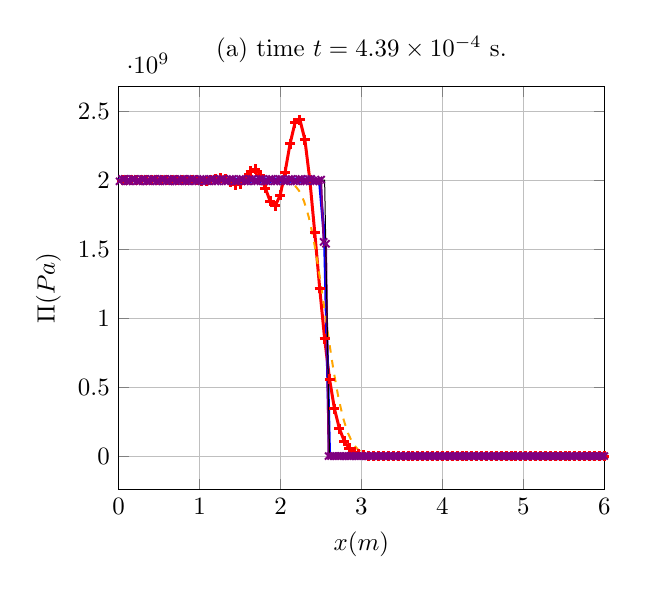
\begin{tikzpicture}[scale=0.9]
\begin{axis}[xlabel=$x (m)$,ylabel=$\Pi (Pa)$,ymajorgrids=true,xmajorgrids=true,legend pos= south west,title={(a) time $t = 4.39\times 10^{-4} $ s.},xmin=0.,xmax=6.]
\addplot[Red,very thick,mark=+,solid] coordinates {(-0.01889090575892736,2000726227.9548469) (0.04215938121847631,1999333692.2170322) (0.10320950300088187,2000564307.210718) (0.1642595721497595,1999551619.5161746) (0.22530959528412595,2000366086.7014122) (0.2863596365377364,1999918681.081198) (0.34740962154368255,1999967513.1983385) (0.4084596019243027,1999982956.3759255) (0.4695095542813397,1999789300.767052) (0.5305595706356425,2000638143.0446692) (0.5916096101001108,2000058185.8142667) (0.6526595840065709,2000089500.8199706) (0.7137094080712463,1998731982.696904) (0.7747591964204517,1999802718.761434) (0.8358092400792819,2001103352.5160503) (0.8968596075653851,2002797653.0377228) (0.9579099107745452,2000545034.2858593) (1.0189595027783396,1996318945.1727874) (1.0800083591701581,1993841183.3513687) (1.1410574970379839,1998917122.885443) (1.2021083083094746,2009171450.4722426) (1.2631608670075336,2014924382.2673836) (1.324213039463032,2005656899.5451016) (1.385261769152474,1983449039.423849) (1.4463061626617941,1966015537.327388) (1.507349635271763,1975043578.4303389) (1.5683984989928055,2015342835.6991093) (1.6294570537824011,2063738687.704247) (1.6905226695860884,2079996363.0337298) (1.7515852284367635,2035769364.3281224) (1.8126325838500514,1940918000.2995517) (1.8736591534269504,1845811486.1301281) (1.9346719362907874,1815039899.0369656) (1.9956894703716108,1889210362.9092839) (2.0567336535453324,2058642788.6612728) (2.117818634233786,2262898814.531011) (2.178942416069636,2414862117.653746) (2.240085148148831,2437155605.434466) (2.301214705448431,2293758990.699916) (2.3622968082809916,2001786574.9585006) (2.4233050712621194,1618923825.3431814) (2.4842269247483553,1216053195.9451652) (2.5450639204752132,851463994.3153192) (2.605827780198291,557925039.8409315) (2.66653493894023,343357124.31856114) (2.7272019233986486,199050644.20604298) (2.7878426090238304,108945510.80319592) (2.8484672666547697,56388618.61462657) (2.9090827809076343,27631268.92148142) (2.9696933946574,12828198.479249047) (3.030301534387653,5645398.76980634) (3.0909084955126,2355626.776140429) (3.15151492615744,932070.1392538762) (3.212121131032279,349709.3400203979) (3.2727272450009446,124397.82639027077) (3.333333324329144,41941.30302034219) (3.3939393911637925,13397.315005244573) (3.4545454537338864,4052.370067713768) (3.515151514926613,1159.9211676619566) (3.5757575756985602,313.92767018390856) (3.6363636363489893,80.26085778895391) (3.6969696969662627,19.36314356717398) (3.7575757575749984,4.402469841671484) (3.8181818181816607,0.9419729953317703) (3.878787878787848,0.1893869676468267) (3.9393939393939337,0.03568940015314253) (3.999999999999999,0.006277030177688385) (4.0606060606060606,0.0010162810763876433) (4.121212121212121,0.00011956247957501687) (4.181818181818182,0.0) (4.242424242424242,0.0) (4.303030303030303,0.0) (4.363636363636363,0.0) (4.424242424242425,0.0) (4.484848484848485,0.0) (4.545454545454546,0.0) (4.606060606060606,0.0) (4.666666666666667,0.0) (4.7272727272727275,0.0) (4.787878787878788,0.0) (4.848484848484849,0.0) (4.909090909090909,0.0) (4.96969696969697,0.0) (5.03030303030303,0.0) (5.090909090909091,0.0) (5.151515151515151,0.0) (5.212121212121212,0.0) (5.2727272727272725,0.0) (5.333333333333334,0.0) (5.3939393939393945,0.0) (5.454545454545455,0.0) (5.515151515151516,0.0) (5.575757575757576,0.0) (5.636363636363637,0.0) (5.696969696969697,0.0) (5.757575757575758,0.0) (5.818181818181818,0.0) (5.878787878787879,0.0) (5.9393939393939394,0.0) (6.0,0.0) };
\addplot[Blue,very thick,mark=none,solid] coordinates {(-0.01905005116856936,2008739016.0347507) (0.04200625800028209,1991261736.4427555) (0.10305754928183601,2008739100.409834) (0.16410893267859902,1991261521.605884) (0.22516022487211998,2008739334.4376273) (0.28621163420310985,1991261157.0218182) (0.3472629006887729,2008739718.3484042) (0.40831433629779745,1991260642.4918854) (0.4693655770844152,2008740252.4789007) (0.5304170389659988,1991259977.710147) (0.591468254064157,2008740937.273132) (0.6525197422102871,1991259162.2632153) (0.713570931632428,2008741773.281487) (0.7746224460325223,1991258195.6316195) (0.8356736097927291,2008742761.1610267) (0.8967251504336042,1991257077.1895308) (0.9577762885477589,2008743901.6730618) (1.0188278554137018,1991255806.2060382) (1.0798789678994447,2008745195.6865165) (1.1409305609721991,1991254381.844086) (1.2019816478489238,2008746644.1731992) (1.2630332671077074,1991252803.1625357) (1.3240843283965613,2008748248.2084675) (1.3851359738180737,1991251069.1156514) (1.4461870095419576,2008750008.9730506) (1.5072386811003957,1991249178.5552225) (1.5682896912839626,2008751927.748467) (1.6293413889510406,1991247130.2292893) (1.690392373620723,2008754005.9189367) (1.7514440973658394,1991244922.7847517) (1.812495056549925,2008756244.9680448) (1.8735468063397946,1991242554.768552) (1.9345977400681083,2008758646.4805305) (1.995649515867116,1991240024.626371) (2.0567004241713285,2008761212.1386473) (2.117752225941453,1991237330.7058423) (2.178803108854988,2008763943.7223768) (2.23985493655583,1991234471.2575831) (2.30090579411386,2008766843.192291) (2.3619576477026816,1991231443.3554277) (2.423008479941872,2008763352.9954166) (2.484060357772498,1983892732.551015) (2.5451094294578325,1563462712.6817071) (2.606060606060606,0.0) (2.666666666666667,0.0) (2.7272727272727275,0.0) (2.787878787878788,0.0) (2.8484848484848486,0.0) (2.909090909090909,0.0) (2.9696969696969697,0.0) (3.0303030303030303,0.0) (3.090909090909091,0.0) (3.1515151515151514,0.0) (3.2121212121212124,0.0) (3.272727272727273,0.0) (3.3333333333333335,0.0) (3.393939393939394,0.0) (3.4545454545454546,0.0) (3.515151515151515,0.0) (3.5757575757575757,0.0) (3.6363636363636367,0.0) (3.6969696969696972,0.0) (3.757575757575758,0.0) (3.8181818181818183,0.0) (3.878787878787879,0.0) (3.9393939393939394,0.0) (4.0,0.0) (4.0606060606060606,0.0) (4.121212121212121,0.0) (4.181818181818182,0.0) (4.242424242424242,0.0) (4.303030303030303,0.0) (4.363636363636363,0.0) (4.424242424242425,0.0) (4.484848484848485,0.0) (4.545454545454546,0.0) (4.606060606060606,0.0) (4.666666666666667,0.0) (4.7272727272727275,0.0) (4.787878787878788,0.0) (4.848484848484849,0.0) (4.909090909090909,0.0) (4.96969696969697,0.0) (5.03030303030303,0.0) (5.090909090909091,0.0) (5.151515151515151,0.0) (5.212121212121212,0.0) (5.2727272727272725,0.0) (5.333333333333334,0.0) (5.3939393939393945,0.0) (5.454545454545455,0.0) (5.515151515151516,0.0) (5.575757575757576,0.0) (5.636363636363637,0.0) (5.696969696969697,0.0) (5.757575757575758,0.0) (5.818181818181818,0.0) (5.878787878787879,0.0) (5.9393939393939394,0.0) (6.0,0.0) };
\addplot[Orange,thick,mark=none,dashed] coordinates {(-0.01889946980668934,2000000476.6320922) (0.011472982262261672,2000001438.4851248) (0.04184684081405173,2000002392.7012472) (0.07221830818119625,2000003356.4999018) (0.1025917130426491,2000004313.5796762) (0.13296300523969845,2000005281.2865465) (0.16333630052391546,2000006243.1661801) (0.19370758569637742,2000007216.7782526) (0.22408085754430615,2000008185.4363225) (0.2544521532603863,2000009167.002689) (0.28482541656310756,2000010144.4770656) (0.3151967209063114,2000011136.1183035) (0.3455699783645009,2000012124.525834) (0.375941289271186,2000013128.4548132) (0.4063145421596361,2000014130.011946) (0.4366858582807102,2000015148.5565734) (0.46705910748905927,2000016165.6025586) (0.49743042788464853,2000017201.230468) (0.5278036740577438,2000018236.2531688) (0.5581749980487619,2000019291.6008966) (0.5885482416749542,2000020347.2658136) (0.6189195687537644,2000021425.1713114) (0.6492928102146956,2000022504.3554904) (0.6796641399908071,2000023607.8955212) (0.7100373795927971,2000024713.7263746) (0.7404087117584984,2000025846.261096) (0.770781949752748,2000026982.1621099) (0.801153284060668,2000028147.3869371) (0.8315265206562344,2000029317.1320484) (0.8618978569046679,2000030519.139193) (0.8922710922772454,2000031726.917393) (0.9226424303005011,2000032970.2716842) (0.9530156645993644,2000034220.765175) (0.9833870042609338,2000035510.5942588) (1.0137602376150086,2000036809.0741432) (1.0441315788021248,2000038151.1810029) (1.0745048113249476,2000039503.6248093) (1.1048761539440453,2000040904.6263094) (1.135249385737295,2000042317.864904) (1.1656207297105001,2000043785.3669105) (1.1959939608663954,2000045267.2687786) (1.2263653061291135,2000046810.0885317) (1.256738536732258,2000048369.7969508) (1.287109883231583,2000049998.2522519) (1.317483113360697,2000051646.4962869) (1.3478544610543197,2000053372.763049) (1.3782276907838837,2000055122.2291121) (1.4085990396392938,2000056960.6600883) (1.4389722690410596,2000058826.1717622) (1.4693436190349667,2000060793.545488) (1.4997168481792058,2000062791.8230162) (1.5300881992973736,2000064911.2737882) (1.560461428254117,2000067066.273204) (1.5908327804937845,2000069397.197215) (1.6212060093376797,2000071787.9900625) (1.6515773627224224,2000074524.9349527) (1.6819505915575537,2000077452.350958) (1.7123219461747121,2000080903.035157) (1.7426951752003998,2000084936.5086977) (1.7730665311339828,2000087540.9977086) (1.803439760589524,2000090978.4911919) (1.8338111168181779,2000077477.0261457) (1.8641843455780502,2000060918.7151618) (1.89455569411346,1999958154.3051436) (1.9249289121352766,1999828194.6022284) (1.9553002169004803,1999383368.9065702) (1.9856733785402865,1998822980.5573165) (2.016044517032017,1997345314.8488786) (2.0464174695217108,1995510656.7783453) (2.076788104100392,1991451764.8388326) (2.1071604354370703,1986509217.5580401) (2.137529784396641,1976980528.1385503) (2.167900564514874,1965628394.4283447) (2.198267080236323,1946149393.6631432) (2.2286345177754954,1923474337.231913) (2.258995557200682,1888386109.4679742) (2.2893566818194317,1848505164.4681375) (2.319708344599485,1792363112.5595503) (2.3500589114299957,1730086099.196376) (2.3803962543095176,1649845080.7546284) (2.410731075812863,1562996199.566734) (2.441048815997596,1460110948.707434) (2.4713625925459266,1351464850.755648) (2.501656185567081,1232676868.5027761) (2.531944653047198,1110279637.2963586) (2.5622113868239693,986331460.2560489) (2.5924723706106327,861678218.7179918) (2.6227120342555033,744346670.210031) (2.652945972784969,629124816.8222382) (2.6831608274884244,527964164.37957025) (2.71337055903147,430909155.97551006) (2.743564662850764,351163528.32019114) (2.7737546123498764,276374743.51695853) (2.8039328190674553,218694935.4413843) (2.8341079548422545,165789527.4489097) (2.8642749709886175,127396775.37849465) (2.8944399082519543,92940066.64930406) (2.9245996662205296,69367708.39847162) (2.9547581309384414,48658784.39870716) (2.9849135418650325,35284991.624521784) (3.015068211540017,23779444.403994165) (3.045221214363269,16758966.548834514) (3.075373824972491,10842273.254041858) (3.1055255924007317,7429200.53377867) (3.1356771679720667,4610317.903746986) (3.165828347947403,3072574.7950721933) (3.195979441069561,1827504.9990729818) (3.2261303619529405,1185127.147576748) (3.2562812464212003,675046.6861063467) (3.2864320612710896,426155.42986476084) (3.3165828619726887,232265.35139310345) (3.346733636544425,142805.4142200062) (3.3768844060203573,74409.37325305404) (3.407035166388237,44577.386497880674) (3.4371859250543553,22185.129789297524) (3.4673366807720183,12956.171896078795) (3.4974874359627095,6152.611330358401) (3.52763819026706,3504.3041958899166) (3.557788944420106,1586.2018885915058) (3.587939698325784,881.5070838911788) (3.618090452191194,379.88885595171956) (3.6482412059925275,206.08344960854643) (3.678391959783931,84.45086513091069) (3.7085427135599374,44.74051898936539) (3.738693467333677,17.410030683202127) (3.7688442211039845,9.011483867110433) (3.798994974873815,3.3249727757824945) (3.8291457286429367,1.6822440876309985) (3.8592964824119647,0.5877093683522783) (3.889447236180857,0.2908357315665427) (3.9195979899497333,0.09612823357834788) (3.9497487437185854,0.04662936703426465) (3.979899497487435,0.014706184987727878) (4.01005025125628,0.0069944050551386675) (4.040201005025126,0.0021521246323503206) (4.0703517587939695,0.001016281076387647) (4.100502512562814,0.0003586874387250511) (4.130653266331658,0.00011956247957501691) (4.160804020100502,5.978123978750844e-05) (4.190954773869347,0.0) (4.221105527638191,0.0) (4.251256281407035,0.0) (4.281407035175879,0.0) (4.311557788944723,0.0) (4.341708542713568,0.0) (4.371859296482412,-5.9781239787508415e-05) (4.402010050251256,0.0) (4.4321608040201,0.0) (4.4623115577889445,0.0) (4.492462311557789,0.0) (4.522613065326633,0.0) (4.552763819095477,0.0) (4.582914572864321,0.0) (4.613065326633166,0.0) (4.64321608040201,0.0) (4.673366834170854,-5.9781239787508415e-05) (4.703517587939698,0.0) (4.733668341708542,0.0) (4.763819095477387,0.0) (4.793969849246231,0.0) (4.824120603015075,0.0) (4.8542713567839195,0.0) (4.884422110552763,0.0) (4.914572864321608,0.0) (4.944723618090452,0.0) (4.974874371859296,0.0) (5.005025125628141,0.0) (5.035175879396984,0.0) (5.065326633165829,0.0) (5.0954773869346734,0.0) (5.125628140703517,0.0) (5.155778894472362,0.0) (5.185929648241205,0.0) (5.21608040201005,0.0) (5.2462311557788945,0.0) (5.276381909547738,-5.9781239787508415e-05) (5.306532663316583,0.0) (5.3366834170854265,-5.9781239787508415e-05) (5.366834170854271,0.0) (5.396984924623116,0.0) (5.427135678391959,0.0) (5.457286432160804,0.0) (5.487437185929648,0.0) (5.517587939698492,0.0) (5.547738693467337,0.0) (5.57788944723618,0.0) (5.608040201005025,5.978123978750844e-05) (5.638190954773869,-5.9781239787508415e-05) (5.668341708542713,0.0) (5.698492462311558,0.0) (5.7286432160804015,0.0) (5.758793969849246,0.0) (5.788944723618091,0.0) (5.819095477386934,-5.9781239787508415e-05) (5.849246231155779,5.978123978750844e-05) (5.879396984924623,0.0) (5.909547738693467,0.0) (5.939698492462312,0.0) (5.969849246231155,0.0) (6.0,0.0) };
\addplot[Purple,thick,mark=x,solid] coordinates {(-0.018953461066473463,1991446661.061328) (0.011194714201811728,1991447340.1765282) (0.04179263124474906,2008553616.6801457) (0.07194754383908661,2008553786.3057418) (0.10253643380986284,1991447493.3310626) (0.13269301032617906,1991447574.3422425) (0.16328078147576108,2008554572.7002) (0.19343774764936655,2008554582.1389053) (0.2240253779425685,1991447859.6478121) (0.25418241511482015,1991447930.5818691) (0.28476989626688765,2008555624.9177055) (0.3149269257596361,2008555623.2558448) (0.3455145674347823,1991448034.9819658) (0.3756715692879528,1991448133.6042144) (0.4062590714943057,2008556842.0924373) (0.4364160416359035,2008556838.9115138) (0.467003771159221,1991448037.4972131) (0.49716070825940945,1991448166.2255507) (0.527748249418257,2008558224.400137) (0.5579051540553267,2008558220.3215702) (0.5884929746851078,1991447868.2226775) (0.6186498466884454,1991448027.2040389) (0.6492374264275679,2008559771.3514504) (0.6793942666629291,2008559766.4251652) (0.7099821771011725,1991447527.543242) (0.7401389854675806,1991447716.7777178) (0.7707266022892127,2008561486.8090549) (0.8008833796675556,2008561481.0619845) (0.8314713783415424,1991447015.2910771) (0.8616281246321296,1991447234.7695084) (0.8922157769826508,2008563372.0888019) (0.922372493064097,2008563365.5949845) (0.9529605783946749,1991446329.7058122) (0.9831172641638408,1991446579.4234667) (1.013704950502113,2008565427.774235) (1.043861606833815,2008565420.8015227) (1.0744497772541894,1991445469.688907) (1.1046064040410184,1991445749.669622) (1.1351941228445261,2008567654.0964527) (1.1653507209569671,2008567647.6765823) (1.195938974915969,1991444434.1637495) (1.2260955442415553,1991444744.559402) (1.2566832940090453,2008570050.2893353) (1.286839835413446,2008570048.467054) (1.3174281713785905,1991443221.7297113) (1.3475846847426682,1991443563.2392223) (1.3781724639980146,2008572611.4914522) (1.4083289501820841,2008572630.206443) (1.4389173666457995,1991441829.765011) (1.469073825519406,1991442205.4102721) (1.4996616328369274,2008575316.3861573) (1.5298180652886002,2008575418.546248) (1.5604065608948054,1991440250.8294203) (1.5905629670328438,1991440673.458793) (1.6211508009003384,2008578078.4761584) (1.651307181902967,2008578512.435198) (1.6818957543055844,1991438457.6398063) (1.7120521100573114,1991438981.576465) (1.7426399679238898,2008580553.9702086) (1.7727962994057174,2008582300.2559524) (1.8033849467032101,1991436340.3404675) (1.833541253464869,1991437194.6760008) (1.8641291340288655,2008581384.4771564) (1.8942854172504617,2008588314.2161562) (1.9248741386090946,1991433444.741186) (1.9550303967770726,1991435593.872973) (1.985618299764926,2008575211.952947) (2.0157745348986764,2008602607.6126542) (2.046363331872024,1991427881.1583545) (2.0765195383045882,1991435378.6636598) (2.1071074672449113,2008540913.448154) (2.1372636502512763,2008649104.02732) (2.167852533779668,1991411780.894133) (2.198008671382919,1991441640.7525687) (2.228596644878877,2008395232.284703) (2.258752754918473,2008822359.8198197) (2.289341773203813,1991352408.047383) (2.3194977696318317,1991475946.8571541) (2.350085866291964,2007809494.577574) (2.3802418153253666,2009495560.7708085) (2.41083116453372,1991111400.0449364) (2.440986728457478,1991626928.107113) (2.471575265426608,1997987384.3139741) (2.5017306963085564,2003928221.7149866) (2.5323193981554217,1552508599.2255695) (2.5624732054671786,1538607374.1694043) (2.5929648241206027,0.000717374877450103) (2.6231155778894473,0.0006575936376625943) (2.6532663316582914,0.0003586874387250511) (2.6834170854271355,0.0003586874387250511) (2.7135678391959797,0.0006575936376625943) (2.743718592964824,0.0006575936376625943) (2.7738693467336684,0.0005978123978750856) (2.8040201005025125,0.0005978123978750856) (2.8341708542713566,0.0005380311580875769) (2.8643216080402008,0.0004782499183000683) (2.8944723618090453,0.00023912495915003393) (2.9246231155778895,0.00023912495915003393) (2.9547738693467336,0.0005380311580875769) (2.9849246231155777,0.0005380311580875769) (3.015075376884422,0.0001793437193625254) (3.0452261306532664,0.0001793437193625254) (3.0753768844221105,0.0005978123978750856) (3.1055276381909547,0.0005380311580875769) (3.135678391959799,0.00023912495915003393) (3.165829145728643,0.00023912495915003393) (3.1959798994974875,0.0004782499183000683) (3.2261306532663316,0.0004184686785125597) (3.2562814070351758,0.0004782499183000683) (3.28643216080402,0.0004782499183000683) (3.316582914572864,5.978123978750844e-05) (3.3467336683417086,0.0) (3.3768844221105527,0.0005978123978750856) (3.407035175879397,0.0005380311580875769) (3.437185929648241,0.00023912495915003393) (3.467336683417085,0.0001793437193625254) (3.4974874371859297,0.0005380311580875769) (3.527638190954774,0.0005380311580875769) (3.557788944723618,0.0005380311580875769) (3.587939698492462,0.0005380311580875769) (3.618090452261306,5.978123978750844e-05) (3.648241206030151,0.00011956247957501691) (3.678391959798995,0.0004782499183000683) (3.708542713567839,0.0004782499183000683) (3.738693467336683,-0.00029890619893754183) (3.7688442211055273,-0.00029890619893754183) (3.798994974874372,0.0005978123978750856) (3.829145728643216,0.0005978123978750856) (3.85929648241206,0.0001793437193625254) (3.8894472361809043,0.00011956247957501691) (3.9195979899497484,0.0001793437193625254) (3.949748743718593,0.00011956247957501691) (3.979899497487437,0.0004184686785125597) (4.010050251256281,0.0004184686785125597) (4.040201005025126,0.0) (4.0703517587939695,-0.0001195624795750168) (4.100502512562814,0.0006575936376625943) (4.130653266331658,0.0005978123978750856) (4.160804020100502,0.0) (4.190954773869347,0.0) (4.221105527638191,0.0002989061989375425) (4.251256281407035,0.00023912495915003393) (4.281407035175879,0.00023912495915003393) (4.311557788944723,0.0001793437193625254) (4.341708542713568,0.0002989061989375425) (4.371859296482412,0.0002989061989375425) (4.402010050251256,-5.9781239787508415e-05) (4.4321608040201,-5.9781239787508415e-05) (4.4623115577889445,0.0006575936376625943) (4.492462311557789,0.0006575936376625943) (4.522613065326633,-0.00032879681883129597) (4.552763819095477,-0.00032879681883129597) (4.582914572864321,0.0008369373570251206) (4.613065326633166,0.0007771561172376117) (4.64321608040201,0.0) (4.673366834170854,-5.9781239787508415e-05) (4.703517587939698,0.0003586874387250511) (4.733668341708542,0.0002989061989375425) (4.763819095477387,-0.00032879681883129597) (4.793969849246231,-0.00029890619893754183) (4.824120603015075,0.0004184686785125597) (4.8542713567839195,0.0003586874387250511) (4.884422110552763,0.0003586874387250511) (4.914572864321608,0.0003586874387250511) (4.944723618090452,0.0004782499183000683) (4.974874371859296,0.0004184686785125597) (5.005025125628141,-0.0001195624795750168) (5.035175879396984,-0.0001195624795750168) (5.065326633165829,0.0005978123978750856) (5.0954773869346734,0.0005978123978750856) (5.125628140703517,0.0) (5.155778894472362,5.978123978750844e-05) (5.185929648241205,0.0006575936376625943) (5.21608040201005,0.0005978123978750856) (5.2462311557788945,-0.00029890619893754183) (5.276381909547738,-0.00029890619893754183) (5.306532663316583,5.978123978750844e-05) (5.3366834170854265,5.978123978750844e-05) (5.366834170854271,0.0002989061989375425) (5.396984924623116,0.00023912495915003393) (5.427135678391959,0.0) (5.457286432160804,-5.9781239787508415e-05) (5.487437185929648,-0.00017934371936252516) (5.517587939698492,-0.00017934371936252516) (5.547738693467337,0.0005978123978750856) (5.57788944723618,0.0005380311580875769) (5.608040201005025,0.0003586874387250511) (5.638190954773869,0.0002989061989375425) (5.668341708542713,-0.00032879681883129597) (5.698492462311558,-0.00032879681883129597) (5.7286432160804015,0.0004782499183000683) (5.758793969849246,0.0004782499183000683) (5.788944723618091,-0.0003885780586188042) (5.819095477386934,-0.0003885780586188042) (5.849246231155779,0.0005978123978750856) (5.879396984924623,0.0005978123978750856) (5.909547738693467,-0.0002391249591500335) (5.939698492462312,-0.0002391249591500335) (5.969849246231155,0.0) (6.0,0.0001793437193625254) };
\addplot[black,thin,mark=none,solid] coordinates {(-0.01905005116856936,2000000000.0000362) (0.04200625800028209,2000000000.0000362) (0.10305754928183601,2000000000.0000362) (0.16410893267859902,2000000000.0000362) (0.22516022487211998,2000000000.0000362) (0.28621163420310985,2000000000.0000362) (0.3472629006887729,2000000000.0000362) (0.40831433629779745,2000000000.0000362) (0.4693655770844152,2000000000.0000362) (0.5304170389659988,2000000000.0000362) (0.591468254064157,2000000000.0000362) (0.6525197422102871,2000000000.0000362) (0.713570931632428,2000000000.0000362) (0.7746224460325223,2000000000.0000362) (0.8356736097927291,2000000000.0000362) (0.8967251504336042,2000000000.0000362) (0.9577762885477589,2000000000.0000362) (1.0188278554137018,2000000000.0000362) (1.0798789678994447,2000000000.0000362) (1.1409305609721991,2000000000.0000362) (1.2019816478489238,2000000000.0000362) (1.2630332671077074,2000000000.0000362) (1.3240843283965613,2000000000.0000362) (1.3851359738180737,2000000000.0000362) (1.4461870095419576,2000000000.0000362) (1.5072386811003957,2000000000.0000362) (1.5682896912839626,2000000000.0000362) (1.6293413889510406,2000000000.0000362) (1.690392373620723,2000000000.0000362) (1.7514440973658394,2000000000.0000362) (1.812495056549925,2000000000.0000362) (1.8735468063397946,2000000000.0000362) (1.9345977400681083,2000000000.0000362) (1.995649515867116,2000000000.0000362) (2.0567004241713285,2000000000.0000362) (2.117752225941453,2000000000.0000362) (2.178803108854988,2000000000.0000362) (2.23985493655583,2000000000.0000362) (2.30090579411386,2000000000.0000362) (2.3619576477026816,2000000000.0000362) (2.423008479941872,2000000000.0000362) (2.484060357772498,2000000000.0000362) (2.5451094294578325,2000000000.0000362) (2.606060606060606,0.0) (2.666666666666667,0.0) (2.7272727272727275,0.0) (2.787878787878788,0.0) (2.8484848484848486,0.0) (2.909090909090909,0.0) (2.9696969696969697,0.0) (3.0303030303030303,0.0) (3.090909090909091,0.0) (3.1515151515151514,0.0) (3.2121212121212124,0.0) (3.272727272727273,0.0) (3.3333333333333335,0.0) (3.393939393939394,0.0) (3.4545454545454546,0.0) (3.515151515151515,0.0) (3.5757575757575757,0.0) (3.6363636363636367,0.0) (3.6969696969696972,0.0) (3.757575757575758,0.0) (3.8181818181818183,0.0) (3.878787878787879,0.0) (3.9393939393939394,0.0) (4.0,0.0) (4.0606060606060606,0.0) (4.121212121212121,0.0) (4.181818181818182,0.0) (4.242424242424242,0.0) (4.303030303030303,0.0) (4.363636363636363,0.0) (4.424242424242425,0.0) (4.484848484848485,0.0) (4.545454545454546,0.0) (4.606060606060606,0.0) (4.666666666666667,0.0) (4.7272727272727275,0.0) (4.787878787878788,0.0) (4.848484848484849,0.0) (4.909090909090909,0.0) (4.96969696969697,0.0) (5.03030303030303,0.0) (5.090909090909091,0.0) (5.151515151515151,0.0) (5.212121212121212,0.0) (5.2727272727272725,0.0) (5.333333333333334,0.0) (5.3939393939393945,0.0) (5.454545454545455,0.0) (5.515151515151516,0.0) (5.575757575757576,0.0) (5.636363636363637,0.0) (5.696969696969697,0.0) (5.757575757575758,0.0) (5.818181818181818,0.0) (5.878787878787879,0.0) (5.9393939393939394,0.0) (6.0,0.0) };
%\legend{mpm,dgmpm,dgmpm 2ppc,dgmpm 2ppc (RK2),exact}
\end{axis}
\end{tikzpicture}
%%% Local Variables:
%%% mode: latex
%%% TeX-master: "../../mainManuscript"
%%% End:
}
  {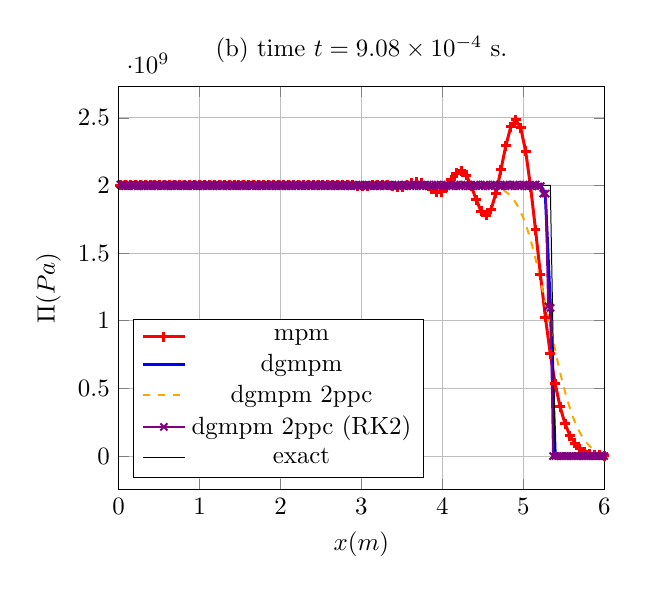
\begin{tikzpicture}[scale=0.9]
\begin{axis}[xlabel=$x (m)$,ylabel=$\Pi (Pa)$,ymajorgrids=true,xmajorgrids=true,legend pos= south west,title={(b) time $t = 9.08\times 10^{-4} $ s.},xmin=0.,xmax=6.]
\addplot[Red,very thick,mark=+,solid] coordinates {(-0.03923052052922343,2000240481.1233327) (0.021819761015892163,1999769738.8663158) (0.0828698927161351,2000218983.1347811) (0.1439199523557292,1999809950.54204) (0.20496998238621425,2000170838.6984289) (0.266019997207666,1999872129.80287) (0.32706999231126516,2000106436.8640933) (0.38811998365041567,1999944280.2454906) (0.449169959029736,2000038581.9512253) (0.510219934372632,2000013690.4345057) (0.5712698969291694,1999979089.5826085) (0.6323198600631447,2000070050.8467832) (0.6933698136476303,1999936253.3022394) (0.7544197669696648,2000107588.3199086) (0.8154697138768967,1999913395.649439) (0.876519659147888,2000125156.8768682) (0.9375696007168677,1999909211.6999958) (0.9986195394150338,2000126157.9927893) (1.059669476515721,1999919755.674749) (1.1207194099155477,2000115626.1187456) (1.1817693429480685,1999938103.4741611) (1.2428192719189772,2000098747.9520392) (1.3038692012782542,1999960657.9597352) (1.3649191269853391,2000083196.644746) (1.4259690532702223,1999982772.5176466) (1.4870189759372838,2000065998.3151865) (1.548068898510965,1999996968.6891499) (1.6091188183068375,2000054865.2647946) (1.670168739008601,2000018826.7281826) (1.731218658453022,2000056284.8743527) (1.7922685772512423,2000025238.8196642) (1.8533184921045645,2000031968.1138716) (1.9143684047609901,2000016400.7497857) (1.975418318053308,2000048568.7818315) (2.0364682364589175,2000073517.7988975) (2.097518157338219,2000081126.454338) (2.158568072062211,2000026752.5138342) (2.2196179727824346,1999962203.1821125) (2.2806678657928665,1999965067.139214) (2.341717771696925,2000088677.3296564) (2.4027677072086253,2000244140.0735695) (2.463817659277123,2000248079.915646) (2.5248675831316487,1999993716.8853536) (2.585917440063807,1999643305.288324) (2.646967250875889,1999579001.41102) (2.7080171068001158,2000062944.273291) (2.7690671011838006,2000852362.1540391) (2.830117219896753,2001206846.0073657) (2.8911672958158867,2000467231.4954524) (2.952217111542271,1998832793.1242473) (3.013266610958221,1997579685.768277) (3.0743160452078344,1998242489.666675) (3.1353658703158658,2001160849.0509126) (3.196416388566518,2004588933.5455565) (3.257467375954363,2005458038.2563794) (3.3185180466647264,2001697102.190524) (3.3795675234732467,1994541487.4730227) (3.440615585708569,1988762645.3894498) (3.5016631438647106,1989935602.9797668) (3.5627119421792885,2000111386.41128) (3.623763471464838,2014923977.0724418) (3.6848176974855837,2024790001.3711026) (3.7458725195458533,2020382377.2601633) (3.8069245712514714,1999447389.7073095) (3.8679711628702065,1970442647.6100123) (3.929012327573847,1949825797.016439) (3.9900516480144432,1953585186.3226125) (4.051095073761827,1987368815.1052973) (4.112148038363928,2040849436.9858987) (4.173212220481733,2090050737.5576959) (4.234283670427938,2107411656.1073942) (4.295353507700337,2075285788.362349) (4.356411206000879,1996293178.97995) (4.417449188621994,1894985293.978191) (4.478466731235185,1809589469.956608) (4.539471418899192,1777676873.8302789) (4.60047747902865,1822118201.7227845) (4.661501591798265,1942507354.7681544) (4.722557637422781,2114144751.4232287) (4.783652041946421,2294062789.964336) (4.844781069302256,2432159789.043516) (4.9059308043019065,2484574935.165112) (4.96707981812872,2425532064.97198) (5.028203724005535,2253708085.122853) (5.0892802390172465,1990804259.1885338) (5.150293249469595,1673238957.9983215) (5.211234847071616,1340859784.348242) (5.272105144435457,1027275994.3558226) (5.332910451399713,754633075.0224329) (5.393660750710443,533012801.80897325) (5.454367310619323,362876107.24577975) (5.515040918237955,238609504.42548501) (5.5756908552374504,151790024.9898157) (5.636324503231241,93541463.05793001) (5.696947375682255,55910425.71914032) (5.7575633798909625,32464567.359246336) (5.818175162719966,18385124.7089494) (5.878784450683184,10291867.039909834) (5.939392341636735,5971073.523642217) (5.999999537141593,4112438.7996382113) };
\addplot[Blue,very thick,mark=none,solid] coordinates {(-0.03942160478635286,2006060116.9510684) (0.021634703667567715,1993940137.594559) (0.08268599644388969,2006060373.9301388) (0.14373737764912256,1993939604.21122) (0.20478867280919388,2006061026.086628) (0.26584007847159263,1993938675.6310308) (0.32689134939619946,2006062073.480748) (0.38794277985880155,1993937351.85318) (0.4489940265576721,2006063516.189758) (0.5100454818139241,1993935632.8617878) (0.571096704298863,2006065354.3060572) (0.6321481843393669,1993933518.6248724) (0.6931993826243398,2006067587.9363937) (0.7542508874368217,1993931009.095019) (0.8153020615377354,2006070217.2044432) (0.876353591107017,1993928104.2093496) (0.9374047410418783,2006073242.2485344) (0.9984562953499471,1993924803.890371) (1.0595074211388207,2006076663.222377) (1.1205590001648187,1993921108.0437915) (1.1816101018298202,2006080480.2947278) (1.2426617055500626,1993917016.5617368) (1.3037127831153568,2006084693.6486328) (1.3647644115033453,1993912529.3202007) (1.4258154649951433,2006089303.4830647) (1.48686711802158,1993907646.1796832) (1.5479181474681376,2006094310.0113149) (1.6089698251009463,1993902366.9880114) (1.6700208305325863,2006099713.4611773) (1.7310725327370886,1993896691.5758796) (1.792123514186276,2006105514.0745523) (1.853175240924819,1993890619.7603688) (1.9142261984258384,2006111712.10775) (1.9752779496581556,1993884151.3441877) (2.0363288832474176,2006118307.831492) (2.097380658930556,1993877286.1154313) (2.1584315686465,2006125301.5292413) (2.21948336873485,1993870023.8487618) (2.28053425461794,2006132693.498629) (2.3415860790632617,1993862364.3047736) (2.4026369411559783,2006140484.0500283) (2.463688789907431,1993854307.2305677) (2.524739628254281,2006148673.5077674) (2.5857915012584574,1993845852.3584197) (2.6468423159059484,2006157262.2078867) (2.7078942131069095,1993836999.410417) (2.7689450041035615,2006166250.4990761) (2.8299969254428645,1993827748.093002) (2.891047692839202,2006175638.7426183) (2.9520996382559384,1993818098.1014004) (3.0131503821044743,2006185427.3114746) (3.074202351535314,1993808049.1178594) (3.13525307189056,2006195616.5906525) (3.196305065269774,1993797600.8137424) (3.2573557621882188,2006206206.9747465) (3.318407779447733,1993786752.8469522) (3.379458452987844,2006217198.8708515) (3.4405104940572713,1993775504.865476) (3.5015611442794836,2006228592.6960747) (3.562613209086164,1993763856.5055692) (3.6236638360528746,2006240388.8765044) (3.684715924521922,1993751807.3932695) (3.745766528297479,2006252587.8494554) (3.806818640351814,1993739357.1445801) (3.8678692210025045,2006265190.0607684) (3.9289213565629106,1993726505.364711) (3.9899719141569547,2006278195.9650536) (4.051024073142108,1993713251.6505055) (4.112074607749643,2006291606.0248404) (4.173126790076167,1993699595.5889838) (4.234177301769245,2006305420.7115803) (4.295229507351752,1993685536.758891) (4.356279996204306,2006319640.5037947) (4.4173322249554365,1993671074.7315753) (4.478382691043292,2006334265.886256) (4.539434942873767,1993656209.068866) (4.600485386274613,2006349297.3502934) (4.661537661093276,1993640939.3284109) (4.72258808188665,2006364735.3943052) (4.783640379600513,1993625265.0586715) (4.844690777867787,2006380580.5203645) (4.905743098382081,1993609185.8030493) (4.966793474206442,2006396833.2363412) (5.027845817424658,1993592701.0995812) (5.088896170891094,2006413494.1091921) (5.149948536715043,1993575783.3857787) (5.2109988679040695,2006188385.7824419) (5.272051199443885,1928173675.83211) (5.333086626305186,1114893331.7484362) (5.3939393939393945,0.0) (5.454545454545455,0.0) (5.515151515151516,0.0) (5.575757575757576,0.0) (5.636363636363637,0.0) (5.696969696969697,0.0) (5.757575757575758,0.0) (5.818181818181818,0.0) (5.878787878787879,0.0) (5.9393939393939394,0.0) (6.0,0.0) };
\addplot[Orange,thick,mark=none,dashed] coordinates {(-0.03917078051451722,2000000162.3641174) (-0.008798328514825843,2000000488.4820786) (0.02157552989991438,2000000813.2866108) (0.051946997059085696,2000001139.558676) (0.08232040164605842,2000001464.592103) (0.11269169349583695,2000001791.172434) (0.14306498836737944,2000002116.5878267) (0.17343627305229423,2000002443.631678) (0.20380954434819964,2000002769.5829566) (0.23418083943507145,2000003097.2461593) (0.26455410204486396,2000003423.8882744) (0.29492540561539754,2000003752.3279023) (0.32529866223778026,2000004079.8172007) (0.3556699722260966,2000004409.1920872) (0.38604322413345515,2000004737.6865525) (0.4164145391877686,2000005068.1573205) (0.4467877872668746,2000005397.8171813) (0.4771591064441345,2000005729.5467284) (0.5075323513364826,2000006060.534245) (0.5379036739539097,2000006393.6881065) (0.5682769161439751,2000006726.1685727) (0.5986482416896831,2000007060.9151359) (0.6290214815546709,2000007395.0570292) (0.6593928096333185,2000007731.5681388) (0.6897660474744984,2000008067.5430918) (0.7201373777728655,2000008405.9942615) (0.7505106138357185,2000008743.9778793) (0.7808819461002032,2000009084.5488696) (0.8112551805873307,2000009424.7210948) (0.8416265146091947,2000009767.5960035) (0.8719997476890129,2000010110.141691) (0.9023710832946423,2000010455.5098622) (0.9327443151082355,2000010800.6187513) (0.9631156521521939,2000011148.6750796) (0.9934888828192661,2000011496.5425496) (1.023860221178728,2000011847.4878132) (1.0542334508024265,2000012198.3157957) (1.0846047903724751,2000012552.357385) (1.114978019042759,2000012906.3543007) (1.1453493597326887,2000013263.7067938) (1.1757225875285224,2000013621.0883734) (1.2060939292591928,2000013981.9742343) (1.2364671562501526,2000014342.964246) (1.2668384989521082,2000014707.6141872) (1.2972117251998054,2000015072.4452546) (1.327583068811835,2000015441.0991797) (1.3579562943711885,2000015810.0127223) (1.3883276388390875,2000016182.9205422) (1.4187008637593828,2000016556.168837) (1.4490722090348958,2000016933.5912306) (1.479445433360601,2000017311.4369278) (1.5098167794005606,2000017693.6460981) (1.540190003171984,2000018076.364191) (1.5705613499376172,2000018463.64511) (1.600934573191448,2000018851.5232396) (1.6313059206478067,2000019244.1745574) (1.6616791434175868,2000019637.514589) (1.6920504915330754,2000020035.8497267) (1.7224237138495884,2000020434.9682348) (1.752795062595561,2000020839.3167174) (1.783168284487177,2000021244.54714) (1.8135396338376049,2000021655.256114) (1.8439128553305595,2000022066.9496617) (1.874284205261732,2000022484.3848658) (1.9046574263803855,2000022902.912099) (1.9350287768706722,2000023327.4603496) (1.9654019976377166,2000023753.2127259) (1.995773348667354,2000024185.283102) (2.026146569104,2000024618.6753104) (2.056517920654903,2000025058.701214) (2.0868911407810526,2000025500.1727536) (2.117262492836659,2000025948.6143074) (2.1476357126710357,2000026398.631942) (2.1780070652161907,2000026855.9786568) (2.2083802847764655,2000027315.038813) (2.2387516377972774,2000027781.8113482) (2.2691248571002074,2000028250.4430869) (2.299496210583961,2000028727.197738) (2.3298694296454614,2000029205.9659374) (2.360240783580518,2000029693.2966387) (2.390614002415777,2000030182.80506) (2.420985356791518,2000030681.3481157) (2.4513585754150644,2000031182.2437081) (2.4817299302217974,2000031692.6813707) (2.512103148647591,2000032205.6581848) (2.5424745038765173,2000032728.723872) (2.5728477221179986,2000033254.5284579) (2.6032190777611506,2000033791.011848) (2.633592295831322,2000034330.4484112) (2.6639636518815353,2000034881.2016294) (2.6943368697930166,2000035435.1385217) (2.724708226243874,2000036001.0829961) (2.7550814440089666,2000036570.4594786) (2.785452800854792,2000037152.5936723) (2.8158260184855197,2000037738.4283779) (2.8461973757213492,2000038337.8370101) (2.8765705932295256,2000038941.2369497) (2.9069419508510856,2000039559.100701) (2.9373151682483614,2000040181.272001) (2.9676865262520598,2000040818.8798575) (2.998059743549965,2000041461.1396496) (3.0284311019329078,2000042119.902398) (3.058804319142925,2000042783.693527) (3.0891756779028725,2000043465.1593158) (3.119548895036467,2000044152.0662634) (3.149920254171894,2000044857.9392831) (3.1802934712405904,2000045569.707488) (3.210664830750652,2000046301.8697186) (3.241038047766071,2000047040.4279282) (3.271409407650652,2000047800.9644024) (3.3017826246245887,2000048568.4518778) (3.332153984884333,2000049359.6807387) (3.3625272018288044,2000050158.4777672) (3.3928985624651316,2000050982.9869034) (3.423271779392468,2000051815.7531936) (3.4536431404076353,2000052676.442854) (3.4840163573305416,2000053546.1624532) (3.514387718727702,2000054446.298109) (3.544760935659359,2000055356.334058) (3.5751322974426225,2000056299.6104584) (3.6055055143967873,2000057253.7731807) (3.6358768765713187,2000058244.4001842) (3.666250093562429,2000059247.0382943) (3.696621456134557,2000060289.8701007) (3.726994673177886,2000061346.020349) (3.7573660361552457,2000062446.766893) (3.7877392532670706,2000063562.4175744) (3.8181106166588106,2000064727.8445463) (3.8484838338566654,2000065910.2265694) (3.878855197673629,2000067147.2274063) (3.9092284149765657,2000068403.7688186) (3.9395997792308908,2000069711.460432) (3.969972996658988,2000071040.1196663) (4.000344361360155,2000072372.298481) (4.030717578929703,2000073715.0698273) (4.061088944065783,2000074840.6027808) (4.091462161766081,2000075910.8957367) (4.1218335272342905,2000075973.490028) (4.152206744942054,2000075715.9219925) (4.182578110329392,2000072017.5705454) (4.212951327539943,2000067131.4477975) (4.243322691511244,2000052136.1276474) (4.273695906596111,2000033486.8974528) (4.304067265361103,1999988181.887949) (4.334440473729889,1999932969.7635126) (4.364811817560196,1999813571.3437288) (4.395185007538841,1999669911.3315077) (4.425556313547598,1999383776.7298186) (4.4559294579562065,1999043281.0910368) (4.4863006763964615,1998409529.043498) (4.516673716815124,1997663436.0152357) (4.547044747257358,1996355344.6753125) (4.577417567129801,1994831959.2009664) (4.607788220571398,1992302969.86891) (4.638160603215137,1989389898.2979999) (4.668530547222314,1984793672.304229) (4.6989021163023,1979557932.6497817) (4.729270803483105,1971684482.5656424) (4.759640947321604,1962815620.4939368) (4.790007533184552,1950076775.4725223) (4.820375320667521,1935888669.9438126) (4.85073858472269,1916391308.5814097) (4.881102688721596,1894921195.4833472) (4.911460980662173,1866658935.7383642) (4.9418196326105,1835890533.9691072) (4.972170870339898,1797058943.0501766) (5.002521873397632,1755266449.2887096) (5.032863617674702,1704664533.4364638) (5.063204441934459,1650828834.6829815) (5.093534060621755,1588261707.5287433) (5.1238620296206765,1522463019.1566145) (5.154176943201123,1449027996.623211) (5.184489497747455,1372692658.5953019) (5.214787471910191,1290836359.622366) (5.245082470974608,1206731514.3493056) (5.275361900847146,1120019487.5397825) (5.305637899924566,1031954086.5330459) (5.335898023815224,944583266.5800234) (5.366154468378211,856867538.3261541) (5.396395461927203,773038830.7005187) (5.426632751210188,689836677.529801) (5.456855682417766,613149742.0165061) (5.487075091582609,537890878.0345305) (5.517281752431922,470906162.1372124) (5.547485236836296,405894014.3081077) (5.5776778950914725,349940731.67696774) (5.607867825779997,296217313.58628106) (5.638048952254623,251444398.38318378) (5.668227839460561,208891324.5259999) (5.698399860557165,174495130.29764324) (5.728570112675359,142092567.12201983) (5.7587352207461455,116627311.01028177) (5.788898966675067,92773016.07205984) (5.8190589997605136,74455848.39195786) (5.8492179810898115,57259214.528929405) (5.879374365625287,44208394.22829007) (5.90952988824298,31705107.093837854) (5.93968362704645,22082669.924264487) (5.9698365523275365,12349931.960094882) (5.999988236235052,4409369.507638947) };
\addplot[Purple,thick,mark=x,solid] coordinates {(-0.03922301604942032,1994135003.8143709) (-0.009074837831142603,1994135327.5382233) (0.021523075320129238,2005865460.1935375) (0.051677994339231634,2005865540.6397502) (0.0822668758008341,1994135396.4583592) (0.11242345978014313,1994135442.2756677) (0.14301122575351569,2005866580.2736385) (0.17316819949872822,2005866583.7764273) (0.20375581897468137,1994135235.3830903) (0.23391286390200003,1994135281.970573) (0.26450034123994165,2005868078.4857993) (0.29465737837952566,2005868076.052185) (0.3252450076005887,1994134650.7495997) (0.3554020172291876,1994134716.185983) (0.38598951715446034,2005869987.9532342) (0.41614649494956335,2005869984.196581) (0.44673421042392686,1994133650.8641272) (0.4768911553029312,1994133736.3200936) (0.5074786957261858,2005872310.7698147) (0.5376356080195605,2005872305.9982176) (0.5682234130066373,1994132236.1149685) (0.5983802927916309,1994132341.6644566) (0.6289678733432371,2005875047.0253694) (0.6591247212380037,2005875041.269826) (0.6897126144378939,1994130406.364448) (0.7198694305893111,1994130532.0101562) (0.750457049772885,2005878196.6928372) (0.7806138348143057,2005878189.968179) (0.8112018146518958,1994128161.431707) (0.8413585687314308,1994128307.172391) (0.8719462249947207,2005881759.749104) (0.9021029487435118,2005881752.0713456) (0.93269101363723,1994125501.1181188) (0.9628477071998897,1994125666.9514115) (0.9934353990033135,2005885736.186498) (1.02359206300724,2005885727.5732303) (1.0541802113876557,1994122425.2141414) (1.0843368459731915,1994122611.1380703) (1.1149245717959766,2005890126.0066001) (1.145081177586202,2005890116.477569) (1.1756694078991365,1994118933.5003204) (1.20582598502954,1994119139.512731) (1.2364137433721918,2005894929.2238271) (1.2665702924608768,2005894918.8010514) (1.297158603170002,1994115025.7430112) (1.3273151243468142,1994115251.8416276) (1.3579029137342808,2005900145.8680048) (1.388059407611098,2005900134.575021) (1.418647797202381,1994110701.6970189) (1.4488042639020475,1994110947.8799276) (1.4793920829061942,2005905775.9789429) (1.5095485230651517,2005905763.8418655) (1.5401369901663489,1994105961.1079912) (1.5702934041634364,1994106227.373129) (1.6008812512548274,2005911819.6044917) (1.6310376400017392,2005911806.6511338) (1.6616261822127902,1994100803.712939) (1.691782545932699,1994101090.0580282) (1.7223704184836093,2005918276.7966) (1.7525267578346984,2005918263.0567758) (1.7831153730505365,1994095229.246782) (1.81327168818946,1994095535.669637) (1.84385958458336,2005925147.5690346) (1.8740158761491597,2005925133.0745907) (1.9046045627390318,1994089237.483962) (1.9347608308802464,1994089563.9823666) (1.9653487495801851,2005932431.753553) (1.9955049949309274,2005932416.5382469) (2.0260937512936668,1994082828.3726115) (2.0562499739975535,1994083174.944045) (2.0868379134903403,2005940128.4045188) (2.116994114177042,2005940112.50405) (2.1475829387283234,1994076002.632435) (2.1777391175363148,1994076369.2744386) (2.2083270763308156,2005948238.0659459) (2.2384832338849914,2005948221.518105) (2.269072125058446,1994068763.590026) (2.29922826149173,1994069150.2999275) (2.3298162381208245,2005956761.6554585) (2.359972354052955,2005956744.5004637) (2.3905613103018015,1994061110.0614216) (2.420717405859752,1994061516.8370643) (2.45130539888087,2005965699.5618157) (2.481461474678868,2005965681.8411288) (2.5120504944773168,1994053037.4510324) (2.5422065506359943,1994053464.2903204) (2.5727945586318346,2005975052.6724114) (2.6029505957595642,2005975034.4297986) (2.633539677604385,1994044544.567231) (2.663695695815098,1994044991.4683108) (2.694283717395741,2005984821.1414673) (2.7244397172916366,2005984802.422394) (2.755028859703366,1994035631.0282984) (2.7851848413913207,1994036097.989225) (2.8157728751957185,2005995004.9483852) (2.8459288392714592,2005994985.8002572) (2.8765180407956676,1994026296.6488297) (2.906673987358701,1994026783.6678703) (2.937262032055926,2006005604.0494888) (2.9674179616952228,2006005584.521593) (2.998007220903698,1994016541.2667468) (3.028163133711092,1994017048.3420172) (3.0587511880014775,2006016618.410417) (3.0889070845589246,2006016598.5542543) (3.119496400050816,1994006364.723129) (3.1496522804421927,1994006891.8527138) (3.180240343058371,2006028048.018772) (3.2103962078583868,2006028027.8874202) (3.240985578261241,1993995766.8365867) (3.271141427545555,1993996314.0189655) (3.3017294972534104,2006039892.8819644) (3.331885331589273,2006039872.530837) (3.3624747555599876,1993984747.4102676) (3.3926305750146017,1993985314.6443734) (3.42321865061413,2006052153.0306427) (3.453374455747092,2006052132.518732) (3.48396393197279,1993973306.2256682) (3.5141197228426364,1993973893.512831) (3.544707803168714,2006064828.5125036) (3.574863580327216,2006064807.9070828) (3.6054531075260225,1993961443.0478823) (3.635608871022857,1993962050.3986511) (3.666196954945923,2006077919.3870173) (3.6963527053248892,2006077898.7828076) (3.7269422822466223,1993949157.6075246) (3.7570980195483576,1993949785.0704486) (3.7876861059750215,2006091425.6997945) (3.8178418307352264,2006091405.2948232) (3.848431456162036,1993936449.554937) (3.878587168412147,1993937097.334268) (3.909175256285717,2006105347.3760405) (3.939330956553215,2006105327.7684526) (3.9699206293001703,1993923318.2738523) (4.000076317607094,1993923987.2069037) (4.030664405908172,2006119683.8346574) (4.060820082773636,2006119667.1966546) (4.0914098016895215,1993909762.099792) (4.121565467125785,1993910455.6078901) (4.15215355487327,2006134432.4522552) (4.182309209390719,2006134427.151202) (4.212898973359856,1993895775.1409583) (4.243054616959861,1993896507.1797674) (4.273642703213922,2006149582.4981947) (4.303798336396806,2006149621.3106256) (4.334388144345157,1993881334.3105564) (4.36454376709732,1993882161.7715528) (4.395131850970583,2006165091.373452) (4.4252874637767405,2006165303.257006) (4.455877314695601,1993866346.531625) (4.486032917511808,1993867501.231569) (4.516620998213603,2006180791.2370899) (4.546776591485469,2006181684.1461263) (4.57736648452554,1993850433.8838644) (4.607522068119923,1993852860.0486372) (4.638110145133578,2006196022.271079) (4.668265719357673,2006199597.6043155) (4.6988556542048805,1993832059.4747472) (4.72901121861128,1993839601.652889) (4.759599292405184,2006208192.2856772) (4.789754846743917,2006222336.4011028) (4.820344825122395,1993804972.4041867) (4.850500367772052,1993833278.5474827) (4.881088442652384,2006207119.6017978) (4.9112439710457245,2006262908.8673177) (4.941834002729241,1993743755.6062326) (4.97198951079214,1993856492.9333005) (5.002577606347889,2006152814.089386) (5.0327330818177884,2006372707.4450974) (5.063323208674937,1993545112.6047575) (5.09347862854396,1994001236.0147953) (5.124066825570078,2005887534.1138701) (5.15422213702806,2006754086.50732) (5.184812529057544,1992634221.3360858) (5.2149676447418924,1994471882.9187949) (5.245556232946693,1938971680.4954917) (5.275710927344704,1939500363.5698178) (5.306287365314434,1107312826.0054393) (5.336440679759463,1095683477.6733737) (5.366834170854271,0.0006575936376625943) (5.396984924623116,0.0006575936376625943) (5.427135678391959,0.0005380311580875769) (5.457286432160804,0.0004782499183000683) (5.487437185929648,0.0005380311580875769) (5.517587939698492,0.0004782499183000683) (5.547738693467337,0.0005380311580875769) (5.57788944723618,0.0004782499183000683) (5.608040201005025,0.00023912495915003393) (5.638190954773869,0.00023912495915003393) (5.668341708542713,0.0003586874387250511) (5.698492462311558,0.0003586874387250511) (5.7286432160804015,0.0005978123978750856) (5.758793969849246,0.0005978123978750856) (5.788944723618091,0.00023912495915003393) (5.819095477386934,0.00023912495915003393) (5.849246231155779,0.0003586874387250511) (5.879396984924623,0.0003586874387250511) (5.909547738693467,0.0004782499183000683) (5.939698492462312,0.0004782499183000683) (5.969849246231155,0.0) (6.0,0.0001793437193625254) };
\addplot[black,thin,mark=none,solid] coordinates {(-0.03942160478635286,2000000000.0000362) (0.021634703667567715,2000000000.0000362) (0.08268599644388969,2000000000.0000362) (0.14373737764912256,2000000000.0000362) (0.20478867280919388,2000000000.0000362) (0.26584007847159263,2000000000.0000362) (0.32689134939619946,2000000000.0000362) (0.38794277985880155,2000000000.0000362) (0.4489940265576721,2000000000.0000362) (0.5100454818139241,2000000000.0000362) (0.571096704298863,2000000000.0000362) (0.6321481843393669,2000000000.0000362) (0.6931993826243398,2000000000.0000362) (0.7542508874368217,2000000000.0000362) (0.8153020615377354,2000000000.0000362) (0.876353591107017,2000000000.0000362) (0.9374047410418783,2000000000.0000362) (0.9984562953499471,2000000000.0000362) (1.0595074211388207,2000000000.0000362) (1.1205590001648187,2000000000.0000362) (1.1816101018298202,2000000000.0000362) (1.2426617055500626,2000000000.0000362) (1.3037127831153568,2000000000.0000362) (1.3647644115033453,2000000000.0000362) (1.4258154649951433,2000000000.0000362) (1.48686711802158,2000000000.0000362) (1.5479181474681376,2000000000.0000362) (1.6089698251009463,2000000000.0000362) (1.6700208305325863,2000000000.0000362) (1.7310725327370886,2000000000.0000362) (1.792123514186276,2000000000.0000362) (1.853175240924819,2000000000.0000362) (1.9142261984258384,2000000000.0000362) (1.9752779496581556,2000000000.0000362) (2.0363288832474176,2000000000.0000362) (2.097380658930556,2000000000.0000362) (2.1584315686465,2000000000.0000362) (2.21948336873485,2000000000.0000362) (2.28053425461794,2000000000.0000362) (2.3415860790632617,2000000000.0000362) (2.4026369411559783,2000000000.0000362) (2.463688789907431,2000000000.0000362) (2.524739628254281,2000000000.0000362) (2.5857915012584574,2000000000.0000362) (2.6468423159059484,2000000000.0000362) (2.7078942131069095,2000000000.0000362) (2.7689450041035615,2000000000.0000362) (2.8299969254428645,2000000000.0000362) (2.891047692839202,2000000000.0000362) (2.9520996382559384,2000000000.0000362) (3.0131503821044743,2000000000.0000362) (3.074202351535314,2000000000.0000362) (3.13525307189056,2000000000.0000362) (3.196305065269774,2000000000.0000362) (3.2573557621882188,2000000000.0000362) (3.318407779447733,2000000000.0000362) (3.379458452987844,2000000000.0000362) (3.4405104940572713,2000000000.0000362) (3.5015611442794836,2000000000.0000362) (3.562613209086164,2000000000.0000362) (3.6236638360528746,2000000000.0000362) (3.684715924521922,2000000000.0000362) (3.745766528297479,2000000000.0000362) (3.806818640351814,2000000000.0000362) (3.8678692210025045,2000000000.0000362) (3.9289213565629106,2000000000.0000362) (3.9899719141569547,2000000000.0000362) (4.051024073142108,2000000000.0000362) (4.112074607749643,2000000000.0000362) (4.173126790076167,2000000000.0000362) (4.234177301769245,2000000000.0000362) (4.295229507351752,2000000000.0000362) (4.356279996204306,2000000000.0000362) (4.4173322249554365,2000000000.0000362) (4.478382691043292,2000000000.0000362) (4.539434942873767,2000000000.0000362) (4.600485386274613,2000000000.0000362) (4.661537661093276,2000000000.0000362) (4.72258808188665,2000000000.0000362) (4.783640379600513,2000000000.0000362) (4.844690777867787,2000000000.0000362) (4.905743098382081,2000000000.0000362) (4.966793474206442,2000000000.0000362) (5.027845817424658,2000000000.0000362) (5.088896170891094,2000000000.0000362) (5.149948536715043,2000000000.0000362) (5.2109988679040695,2000000000.0000362) (5.272051199443885,2000000000.0000362) (5.333086626305186,2000000000.0000362) (5.3939393939393945,0.0) (5.454545454545455,0.0) (5.515151515151516,0.0) (5.575757575757576,0.0) (5.636363636363637,0.0) (5.696969696969697,0.0) (5.757575757575758,0.0) (5.818181818181818,0.0) (5.878787878787879,0.0) (5.9393939393939394,0.0) (6.0,0.0) };
\legend{mpm,dgmpm,dgmpm 2ppc,dgmpm 2ppc (RK2),exact}
\end{axis}
\end{tikzpicture}
%%% Local Variables:
%%% mode: latex
%%% TeX-master: "../../mainManuscript"
%%% End:
}
  \caption{shock stress lower shock $5\sigma^y$}
  \label{fig:he_low_shock}
\end{figure}

%%% Local Variables:
%%% mode: latex
%%% TeX-master: "../mainManuscript"
%%% End:


\subsection{Problems in two space dimensions}
\label{subsec:he_plate}


\begin{figure}[h!]
  \centering
  \begin{tikzpicture}[scale=0.8]
  \begin{groupplot}[group style={group size=2 by 4,
      ylabels at=edge left, yticklabels at=edge left,
      horizontal sep=4.ex,
      vertical sep=4ex,},
    enlargelimits=0,
    xmin=0.,xmax=10., ymin=-0.,ymax=2.
    ,axis equal image
    ,axis on top,scale only axis,xtick=\empty,ytick=\empty,width=0.45\linewidth,
    ,colorbar style={
      title style={
        font=\scriptsize,
        at={(-2.,-1.25)},
        anchor=north west
      },yticklabel style={font=\scriptsize}
      ,at={(current axis.south east)},anchor=south west
    }]
    %% FIRST ROW (time 1 = 3.5e-4s)
    %%% RANGE -2.0e7 -- 2.9e8
    \nextgroupplot[title={(a) $t= 9.94 \times 10^{-4}\:s$},ylabel={dgmpm (1ppc)},ylabel style={font=\footnotesize}]\addplot graphics[xmin=-0.,xmax=10., ymin=-0.,ymax=2.] {chapter4/pngFigures/PW_dgmpm1ppc_65.png};
    \nextgroupplot[title={(b) $t= 2.54 \times 10^{-4}\:s$},ylabel={\color{white}dgmpm (1pc)},ylabel style={font=\footnotesize}]\addplot graphics[xmin=-0.,xmax=10., ymin=-0.,ymax=2.] {chapter4/pngFigures/PW_dgmpm1ppc_132.png};

    \nextgroupplot[ylabel={dgmpm (4ppc)},ylabel style={font=\footnotesize}]\addplot graphics[xmin=0.,xmax=10., ymin=-0.,ymax=2.] {chapter4/pngFigures/PW_dgmpm4ppc_65.png};
    \nextgroupplot[ylabel={\color{white}dgmpm (4ppc)},ylabel style={font=\footnotesize}]\addplot graphics[xmin=-0.,xmax=10., ymin=-0.,ymax=2.] {chapter4/pngFigures/PW_dgmpm4ppc_132.png};
    
    \nextgroupplot[ylabel={mpm (1ppc)},ylabel style={font=\footnotesize}]\addplot graphics[xmin=0.,xmax=10., ymin=-0.,ymax=2.] {chapter4/pngFigures/PW_mpm1ppc_65.png};
    \nextgroupplot[,ylabel={\color{white}mpm (1ppc)},ylabel style={font=\footnotesize}]\addplot graphics[xmin=-0.,xmax=10., ymin=-0.,ymax=2.] {chapter4/pngFigures/PW_mpm1ppc_132.png};
    
    \nextgroupplot[ylabel={mpm (4ppc)},ylabel style={font=\footnotesize},colorbar horizontal,colorbar  style={
      title style={yshift=-1.5cm},
      title= {$\Pi_{11}\: (GPa)$},
      xtick={0.,20.},
      xticklabels={-6.2,0},
    }]
    %\addplot[scatter,scatter src=y,mark size=0.pt] coordinates {(0.,-5.7e-2) (0.,2.9e-1)};% Fake extreme values to fix scale
    \addplot[scatter,scatter src=x,mark size=0.pt] coordinates {(0.,0.) (20.,0.)};% Fake extreme values to fix scale
    \addplot graphics[xmin=0.,xmax=10., ymin=-0.,ymax=2.] {chapter4/pngFigures/PW_mpm4ppc_65.png};
    
    \nextgroupplot[colorbar horizontal,colorbar style={
      title= {$\Pi_{11}\: (GPa)$},
      title style={yshift=-1.5cm},
      xtick={0.,20.},
      xticklabels={-6.8,0},
    },ylabel={\color{white}mpm (4ppc)},ylabel style={font=\footnotesize}]
    \addplot[scatter,scatter src=x,mark size=0.pt] coordinates {(0.,0.) (20.,0.)};% Fake extreme values to fix scale
    \addplot graphics[xmin=-0.,xmax=10., ymin=-0.,ymax=2.] {chapter4/pngFigures/PW_mpm4ppc_132.png};   
    

    % \nextgroupplot[title={(c) DGMPM 4ppc}]\addplot graphics[xmin=-0.,xmax=1., ymin=-0.,ymax=1.] {chapter4/pngFigures/dgmpm4ppc_stress_115.png};
    % \nextgroupplot[title={(d) MPM 1ppc},
    % colorbar,colorbar style={
    % title= {$\sigma_{11}\: (MPa)$},
    %   ytick={-5.7e-2,2.e-1,2.9e-1},
    %   yticklabels={-57,200,290},
    % }]
    % \addplot[scatter,scatter src=y,mark size=0.pt] coordinates {(0.,-5.7e-2) (0.,2.9e-1)};% Fake extreme values to fix scale
    % \addplot graphics[xmin=-0.,xmax=1., ymin=-0.,ymax=1.] {chapter4/pngFigures/mpm_stress_115.png};

    % %% SECOND ROW (time 2 =1.e-3s)
    % %%% RANGE -4.4e7 -- 4.2e8
    % \nextgroupplot[ylabel={$t=1.0\times 10^{-3} \:s$}]\addplot graphics[xmin=0.,xmax=1., ymin=-0.,ymax=1.] {chapter4/pngFigures/fem_stress_338.png};
    % \nextgroupplot[]\addplot graphics[xmin=-0.,xmax=1., ymin=-0.,ymax=1.] {chapter4/pngFigures/dgmpm1ppc_stress_338.png};
    % \nextgroupplot[]\addplot graphics[xmin=-0.,xmax=1., ymin=-0.,ymax=1.] {chapter4/pngFigures/dgmpm4ppc_stress_338.png};
    % \nextgroupplot[colorbar,colorbar style={
    %   title= {$\sigma_{11}\: (MPa)$},
    %   ytick={-4.3e-2,2.e-1,4.8e-1},
    %   yticklabels={-43,200,480},
    % }]
    % \addplot[scatter,scatter src=y,mark size=0.pt] coordinates {(0.,-4.3e-2) (0.,4.8e-1)};% Fake extreme values to fix scale
    % \addplot graphics[xmin=-0.,xmax=1., ymin=-0.,ymax=1.] {chapter4/pngFigures/mpm_stress_338.png};
    
  \end{groupplot}
\end{tikzpicture}



%%% Local Variables:
%%% mode: latex
%%% TeX-master: "../../mainManuscript"
%%% End:

  % {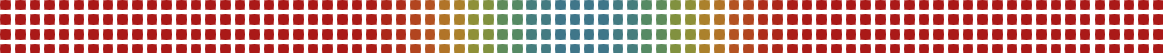
\includegraphics[width=0.5\textwidth]{chapter4/pngFigures/PW_dgmpm4ppc_65.png}}
  % 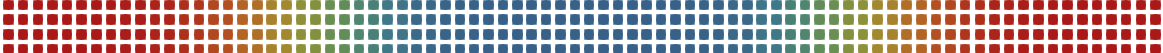
\includegraphics[width=0.5\textwidth]{chapter4/pngFigures/PW_dgmpm4ppc_132.png}
  \caption{test}
  \label{fig:2dplaneWave_stress}
\end{figure}


%%% Local Variables:
%%% mode: latex
%%% TeX-master: "../mainManuscript"
%%% End:

\subsubsection*{Two-dimensional plane strain problem}
% A two-dimensional rectangular plate made of the compressible hyperelastic neo-Hookean material is considered here in the plane strain case.
% Unlike for the Saint-Venant-Kirchhoff model, the polyconvexity of the neo-Hookean stored energy function ensures the hyperbolicity of the problem (see section \ref{sec:constitutive-equations}).
%Geometry, boundary and loading conditions are given in figure \ref{fig:2d_heDomain}.
% \begin{figure}[h!]
%   \centering
%   \begin{tikzpicture}[scale=0.7]
  \draw[thick] (0,0) --(4,0)--(4,3)--(0,3)--(0,0);
  \foreach \x in {0.5,1.,...,3.5} 
  \draw(\x,-0.2)circle(0.2);
  \foreach \x in {0.25,0.75,...,2.75} 
  \draw(4.2,\x)circle(0.2);
  \draw(0,-0.4)--(4.,-0.4);
  \draw(4.4,0)--(4.4,3);
  \fill [pattern=north east lines](0.0,-0.8)rectangle+(4,0.4);
  \fill [pattern=north east lines](4.4,0.)rectangle+(0.4,3);
  \draw[>=stealth,<->](5.1,0)--node[right=1pt]{\footnotesize $h=3 \: m$}(5.1,3);
  \draw[>=stealth,<->](0,3.1)--node[above=1pt]{\footnotesize $l=4 \: m$}(4,3.1);
  \draw[>=stealth,<->](0.1,0)--node[right=1pt]{\footnotesize $a=1 \: m$}(0.1,1);
  \foreach \x in {0.,0.25,...,1} 
  \draw[>=stealth,<-] (-0.5,\x)--(0.,\x);
  \node(a)at(-1.2,0.75){\footnotesize $v_1=v^d$}; 
  \draw[>=stealth,->](-1.5,2)--(-0.5,2)node(a)[anchor=north]{\footnotesize $\vect{e}_1$};
  \draw[>=stealth,->](-1.5,2)--(-1.5,3)node(a)[anchor=south]{\footnotesize $\vect{e}_2$};
\end{tikzpicture}

%%% Local Variables:
%%% mode: latex
%%% TeX-master: "../../mainManuscript"
%%% End:
%   \caption{Geometry, boundary and loading conditions of the two-dimensional problem in plane strain with a hyperelastic neo-Hookean material.}
%   \label{fig:2d_heDomain}
% \end{figure}
The plane strain problem studied in sections \ref{subsec:el_planestrain} and \ref{subsec:ep_planestrain} is now considered in a compressible hyperelastic neo-Hookean material submitted to an imposed velocity $v_1=-1000 \: m/s$ on the bottom part of its left end.
The solid is discretized such that material points are equivalent to $Q1$-finite element nodes.
Thus, the plate is represented with $l \times h \equiv 28 \times 28$ material points, only with the 1ppc configuration.
The finite element computation is performed with the software \textit{Abaqus} \cite{Abaqus} using an explicit time discretization with no artificial viscosity added.
These numerical results are compared to those obtained from MPM and DGMPM using CTU computations.
The Courant number is set to unity in DGMPM and to $0.5$ in MPM leading to \textit{average} time steps $\Delta t_{CTU}=1.41 \times 10^{-5}s$ and $\Delta t_{MPM}=6.13 \times 10^{-6}s$, whereas the \textit{constant} time step used in the FEM simulation is $\Delta t_{FEM}=1.27 \times 10^{-5} s$.
Figure \ref{fig:2dhe_stress} shows numerical results in terms of the Cauchy stress tensor isovalues exported from Abaqus to the software Paraview \cite{Paraview} with the code developed in \cite{Export_Abaqus}, particularized to the present two-dimensional plane strain case.
Cauchy stress is plotted on the current configuration in such a way that figure \ref{fig:2dhe_stress} also enables the comparison of the deformed shape of the body.
\begin{figure}[h!]
  \centering
  \begin{tikzpicture}[scale=0.9]
  \begin{groupplot}[group style={group size=3 by 3,
      ylabels at=edge left, yticklabels at=edge left,
      horizontal sep=1.ex,
      vertical sep=2ex,},
    enlargelimits=0,
    xmin=0.,xmax=1., ymin=-0.,ymax=1.
    ,axis on top,scale only axis,xtick=\empty,ytick=\empty,width=0.25\linewidth,
    colorbar style={
      title style={
        font=\scriptsize,
        at={(1,.5)},
        anchor=north west
      },yticklabel style={font=\scriptsize}
      ,at={(current axis.south east)},anchor=south west
    }]
    %% FIRST ROW (time 1 = 2.3e-4s)
    %%% RANGE -6.5e9 -- 100e9
    \nextgroupplot[ylabel={$t=1.8\times 10^{-4} \:s$},title={(a) FEM}]\addplot graphics[xmin=0.,xmax=1., ymin=-0.,ymax=1.] {chapter4/pngFigures/he_fem_stress53.png};
    \nextgroupplot[title={(a) DGMPM}]\addplot graphics[xmin=0.,xmax=1., ymin=-0.,ymax=1.] {chapter4/pngFigures/he_dgmpm_stress53.png};
    \nextgroupplot[title={(c) MPM},
    colorbar,colorbar style={
      title= {$\sigma_{11}\: (GPa)$},
      ytick={-0.28,10},
      yticklabels={-2.8,100},
    }]
    \addplot[scatter,scatter src=y,mark size=0.pt] coordinates {(0.,-.28) (0.,10)};% Fake extreme values to fix scale
    \addplot graphics[xmin=-0.,xmax=1., ymin=-0.,ymax=1.] {chapter4/pngFigures/he_mpm_stress53.png};

    %% SECOND ROW (time 2 =6.5e-4s)
    %%% RANGE -7.1e9 -- 210e9
    \nextgroupplot[ylabel={$t=5.0\times 10^{-4} \:s$}]\addplot graphics[xmin=0.,xmax=1., ymin=-0.,ymax=1.] {chapter4/pngFigures/he_fem_stress176.png};
    \nextgroupplot[]\addplot graphics[xmin=0.,xmax=1., ymin=-0.,ymax=1.] {chapter4/pngFigures/he_dgmpm_stress176.png};
    \nextgroupplot[colorbar,colorbar style={
      title= {$\sigma_{11}\: (GPa)$},
      ytick={-0.42,19.},
      yticklabels={-4.2,190},
    }]
    \addplot[scatter,scatter src=y,mark size=0.pt] coordinates {(0.,-0.42) (0.,19)};% Fake extreme values to fix scale
    \addplot graphics[xmin=-0.,xmax=1., ymin=-0.,ymax=1.] {chapter4/pngFigures/he_mpm_stress176.png};

    %% THIRD ROW (time 2 =1.4e-3s)
    %%% RANGE -5.9e9 -- 330e9
    \nextgroupplot[ylabel={$t=1.0\times 10^{-3} \:s$}]\addplot graphics[xmin=0.,xmax=1., ymin=-0.,ymax=1.] {chapter4/pngFigures/he_fem_stress444.png};
    \nextgroupplot[]\addplot graphics[xmin=0.,xmax=1., ymin=-0.,ymax=1.] {chapter4/pngFigures/he_dgmpm_stress444.png};
    \nextgroupplot[colorbar,colorbar style={
      title= {$\sigma_{11}\: (GPa)$},
      ytick={-0.75,31.},
      yticklabels={-7.5,310},
    }]
    \addplot[scatter,scatter src=y,mark size=0.pt] coordinates {(0.,-0.75) (0.,31.)};% Fake extreme values to fix scale
    \addplot graphics[xmin=-0.,xmax=1., ymin=-0.,ymax=1.] {chapter4/pngFigures/he_mpm_stress444.png};
    
  \end{groupplot}
\end{tikzpicture}



%%% Local Variables:
%%% mode: latex
%%% TeX-master: "../mainManuscript"
%%% End:

  \caption{Isovalues of Cauchy stress tensor component $\sigma_{11}$ in a two-dimensional plate made of a neo-Hookean material, submitted to a velocity $\vect{v}\cdot\vect{e}_1=-1000 \: m/s$ on a part of its left end.}
  \label{fig:2dhe_stress}
\end{figure}
\begin{figure}[h!]
  \centering
  \begin{tikzpicture}
  \begin{groupplot}[group style={group size=3 by 1, % 3 columns 2 rows
ylabels at=edge left, yticklabels at=edge left,horizontal sep=2.ex,vertical sep=3.ex,
xticklabels at=edge bottom,xlabels at=edge bottom},
ymajorgrids=true,xmajorgrids=true,ylabel=$\sigma_{12} \: (Pa)$,
axis on top,scale only axis,width=0.28\linewidth, every x tick scale label/.style={at={(xticklabel* cs:1.05,0.75cm)},anchor=near yticklabel},
every y tick scale label/.style={at={(yticklabel* cs:1.1,-0.8cm)},anchor=near yticklabel}]
%%%%%%%%%%%%%%%%%%%%
\nextgroupplot[ylabel=$\sigma_{11} \:(Pa)$,title={(a) $t = 1.8 \times 10^{-4}\: s$},xlabel=$x \: (m)$,ymin=-7.5e9,ymax=100.e9]
\addplot[Red,very thick,no markers] table[x=Points:0,y=PK2:0] {chapter4/csvFiles/he_fem31.csv};
\addplot[Blue,very thick,mark=+,only marks,mark size=3pt] table[x=Points:0,y=P_11] {chapter4/csvFiles/he_dgmpm31.csv};
\addplot[Orange,very thick,mark=x,only marks,mark size=3pt] table[x=Points:0,y=mpm_S11] {chapter4/csvFiles/he_mpm31.csv};

\nextgroupplot[title={(b) $t = 5.0 \times 10^{-4}\: s$},xlabel=$x \: (m)$,ymin=-7.5e9,ymax=100.e9,ytick scale label code/.code={}]
\addplot[Red,very thick,no markers] table[x=Points:0,y=PK2:0] {chapter4/csvFiles/he_fem176.csv};
\addplot[Blue,very thick,mark=+,only marks,mark size=3pt] table[x=Points:0,y=P_11] {chapter4/csvFiles/he_dgmpm176.csv};
\addplot[Orange,very thick,mark=x,only marks,mark size=3pt] table[x=Points:0,y=mpm_S11] {chapter4/csvFiles/he_mpm176.csv};


\nextgroupplot[title={(c) $t = 1.0 \times 10^{-3}\: s$},xlabel=$x \: (m)$,ymin=-7.5e9,ymax=100.e9,ytick scale label code/.code={}]
\addplot[Red,very thick,no markers] table[x=Points:0,y=PK2:0] {chapter4/csvFiles/he_fem444.csv};
\addplot[Blue,very thick,mark=+,only marks,mark size=3pt] table[x=Points:0,y=P_11] {chapter4/csvFiles/he_dgmpm444.csv};
\addplot[Orange,very thick,mark=x,only marks,mark size=3pt] table[x=Points:0,y=mpm_S11] {chapter4/csvFiles/he_mpm444.csv};

%%%%%%%%%%%%%%%%%%%%%%%%%%%
% \nextgroupplot[ylabel=$v_{1} \: (m/s)$,xlabel=$x \: (m)$,ymin=-1200.,ymax=120,scaled y ticks={real:1.e3},ytick scale label code/.code={$\cdot 10^{3}$}]
% \addplot[Red,very thick,no markers] table[x=Points:0,y=Spatial_velocity:0] {chapter4/csvFiles/he_fem31.csv};
% \addplot[Blue,very thick,mark=+,only marks,mark size=3pt] table[x=Points:0,y=velocity_x] {chapter4/csvFiles/he_dgmpm31.csv};
% \addplot[Orange,very thick,mark=x,only marks,mark size=3pt] table[x=Points:0,y=mpm_V1] {chapter4/csvFiles/he_mpm31.csv};

% \nextgroupplot[xlabel=$x \: (m)$,ymin=-1200.,ymax=120,legend style={at={($(0.75,-0.4)+(0.9cm,0.6cm)$)},legend columns=3}]
% \addplot[Red,very thick,no markers] table[x=Points:0,y=Spatial_velocity:0] {chapter4/csvFiles/he_fem176.csv};
% \addplot[Blue,very thick,mark=+,only marks,mark size=3pt] table[x=Points:0,y=velocity_x] {chapter4/csvFiles/he_dgmpm176.csv};
% \addplot[Orange,very thick,mark=x,only marks,mark size=3pt] table[x=Points:0,y=mpm_V1] {chapter4/csvFiles/he_mpm176.csv};
% \addlegendentry{fem}
% \addlegendentry{dgmpm}
% \addlegendentry{mpm}


% \nextgroupplot[xlabel=$x \: (m)$,ymin=-1200.,ymax=120]
% \addplot[Red,very thick,no markers] table[x=Points:0,y=Spatial_velocity:0] {chapter4/csvFiles/he_fem444.csv};
% \addplot[Blue,very thick,mark=+,only marks,mark size=3pt] table[x=Points:0,y=velocity_x] {chapter4/csvFiles/he_dgmpm444.csv};
% \addplot[Orange,very thick,mark=x,only marks,mark size=3pt] table[x=Points:0,y=mpm_V1] {chapter4/csvFiles/he_mpm444.csv};

  \end{groupplot}
\end{tikzpicture}


%%% Local Variables:
%%% mode: latex
%%% TeX-master: "../../mainManuscript"
%%% End:


  %\begin{tikzpicture}
  \begin{groupplot}[group style={group size=3 by 1, % 3 columns 2 rows
ylabels at=edge left, yticklabels at=edge left,horizontal sep=2.ex,vertical sep=3.ex,
xticklabels at=edge bottom,xlabels at=edge bottom},
ymajorgrids=true,xmajorgrids=true,ylabel=$\sigma_{12} \: (Pa)$,
axis on top,scale only axis,width=0.28\linewidth, every x tick scale label/.style={at={(xticklabel* cs:1.05,0.75cm)},anchor=near yticklabel}]
%%%%%%%%%%%%%%%%%%%%
% \nextgroupplot[ylabel=$\sigma_{11} \:(Pa)$,title={(a) $t = 1.8 \times 10^{-4}\: s$},ymin=-7.5e9,ymax=100.e9]
% \addplot[Red,very thick,no markers] table[x=Points:0,y=PK2:0] {chapter4/csvFiles/he_fem31.csv};
% \addplot[Blue,very thick,mark=+,only marks,mark size=3pt] table[x=Points:0,y=P_11] {chapter4/csvFiles/he_dgmpm31.csv};
% \addplot[Orange,very thick,mark=x,only marks,mark size=3pt] table[x=Points:0,y=mpm_S11] {chapter4/csvFiles/he_mpm31.csv};

% \nextgroupplot[title={(b) $t = 5.0 \times 10^{-4}\: s$},ymin=-7.5e9,ymax=100.e9,ytick scale label code/.code={}]
% \addplot[Red,very thick,no markers] table[x=Points:0,y=PK2:0] {chapter4/csvFiles/he_fem176.csv};
% \addplot[Blue,very thick,mark=+,only marks,mark size=3pt] table[x=Points:0,y=P_11] {chapter4/csvFiles/he_dgmpm176.csv};
% \addplot[Orange,very thick,mark=x,only marks,mark size=3pt] table[x=Points:0,y=mpm_S11] {chapter4/csvFiles/he_mpm176.csv};


% \nextgroupplot[title={(c) $t = 1.0 \times 10^{-3}\: s$},ymin=-7.5e9,ymax=100.e9,ytick scale label code/.code={}]
% \addplot[Red,very thick,no markers] table[x=Points:0,y=PK2:0] {chapter4/csvFiles/he_fem444.csv};
% \addplot[Blue,very thick,mark=+,only marks,mark size=3pt] table[x=Points:0,y=P_11] {chapter4/csvFiles/he_dgmpm444.csv};
% \addplot[Orange,very thick,mark=x,only marks,mark size=3pt] table[x=Points:0,y=mpm_S11] {chapter4/csvFiles/he_mpm444.csv};

%%%%%%%%%%%%%%%%%%%%%%%%%%%
\nextgroupplot[ylabel=$v_{1} \: (m/s)$,xlabel=$x \: (m)$,title={(a) $t = 1.8 \times 10^{-4}\: s$},ymin=-1200.,ymax=120,scaled y ticks={real:1.e3},ytick scale label code/.code={$\cdot 10^{3}$}]
\addplot[Red,very thick,no markers] table[x=Points:0,y=Spatial_velocity:0] {chapter4/csvFiles/he_fem31.csv};
\addplot[Blue,very thick,mark=+,only marks,mark size=3pt] table[x=Points:0,y=velocity_x] {chapter4/csvFiles/he_dgmpm31.csv};
\addplot[Orange,very thick,mark=x,only marks,mark size=3pt] table[x=Points:0,y=mpm_V1] {chapter4/csvFiles/he_mpm31.csv};

\nextgroupplot[title={(b) $t = 5.0 \times 10^{-4}\: s$},xlabel=$x \: (m)$,ymin=-1200.,ymax=120,legend style={at={($(0.75,-0.4)+(0.9cm,0.6cm)$)},legend columns=3}]
\addplot[Red,very thick,no markers] table[x=Points:0,y=Spatial_velocity:0] {chapter4/csvFiles/he_fem176.csv};
\addplot[Blue,very thick,mark=+,only marks,mark size=3pt] table[x=Points:0,y=velocity_x] {chapter4/csvFiles/he_dgmpm176.csv};
\addplot[Orange,very thick,mark=x,only marks,mark size=3pt] table[x=Points:0,y=mpm_V1] {chapter4/csvFiles/he_mpm176.csv};
\addlegendentry{fem}
\addlegendentry{dgmpm}
\addlegendentry{mpm}


\nextgroupplot[title={(c) $t = 1.0 \times 10^{-3}\: s$},xlabel=$x \: (m)$,ymin=-1200.,ymax=120]
\addplot[Red,very thick,no markers] table[x=Points:0,y=Spatial_velocity:0] {chapter4/csvFiles/he_fem444.csv};
\addplot[Blue,very thick,mark=+,only marks,mark size=3pt] table[x=Points:0,y=velocity_x] {chapter4/csvFiles/he_dgmpm444.csv};
\addplot[Orange,very thick,mark=x,only marks,mark size=3pt] table[x=Points:0,y=mpm_V1] {chapter4/csvFiles/he_mpm444.csv};

  \end{groupplot}
\end{tikzpicture}


%%% Local Variables:
%%% mode: latex
%%% TeX-master: "../../mainManuscript"
%%% End:


  \caption{Evolution of longitudinal Cauchy stress $\sigma_{11}$ along the bottom boundary of the domain.}
  \label{fig:he_lineplots_stress}
\end{figure}
At the beginning of the computation (first row in figure \ref{fig:2dhe_stress}), stress profiles are quite similar despite slight oscillations visible in FEM and MPM solutions.
This can also be seen in figure \ref{fig:he_lineplots_stress}, in which stress is plotted along the bottom boundary of the domain.
However, the MPM solution exhibits, as for small strain problems, a concentration of stress in the high gradients region on the left boundary.
%It is worth noticing that the DGMPM shows the same behavior that cannot be seen here due to the attenuation introduced by MPM stress values which are much higher.
It is worth noticing that the DGMPM shows the same behavior that cannot be seen here due to the MPM stress values which are much higher.
The deformed shapes of the plate resulting from the three numerical approaches hence remain close, except at the junction of the loaded and free zones of the left edge.
When the pressure wave reflects on the fixed boundary at time $t=5.0\times 10^{-4}\:s$ (second row in figures \ref{fig:2dhe_stress} and \ref{fig:2dhe_velo}), the stress profiles are still similar, though FEM and MPM solutions oscillate even more.
These spurious oscillations are more significant in the velocity fields depicted in figure \ref{fig:2dhe_velo} as well as in figures \ref{fig:he_lineplots_stress} and \ref{fig:he_lineplots_velo} which depict the velocity along the bottom boundary.
Furthermore, one can see in figure \ref{fig:he_lineplots_velo}\subref{subfig:he_velo2} that the homogeneous Dirichlet boundary condition is not exactly enforced in DGMPM when the incident wave hits the right end.
\begin{figure}[h!]
  \centering
  \begin{tikzpicture}[scale=0.9]
  \begin{groupplot}[group style={group size=3 by 3,
      ylabels at=edge left, yticklabels at=edge left,
      horizontal sep=1.ex,
      vertical sep=2ex,},
    enlargelimits=0,
    xmin=0.,xmax=1., ymin=-0.,ymax=1.
    ,axis on top,scale only axis,xtick=\empty,ytick=\empty,width=0.25\linewidth,
    colorbar style={
      title style={
        font=\scriptsize,
        at={(1,.5)},
        anchor=north west
      },yticklabel style={font=\scriptsize}
      ,at={(current axis.south east)},anchor=south west
    }]
    %% FIRST ROW (time 1 = 2.3e-4s)
    %%% RANGE -1.6e9 -- 7.8e10
    \nextgroupplot[ylabel={$t=2.3\times 10^{-4} \:s$},title={(a) FEM}]\addplot graphics[xmin=0.,xmax=1., ymin=-0.,ymax=1.] {chapter4/pngFigures/he_fem_velo53.png};
    \nextgroupplot[title={(a) DGMPM}]\addplot graphics[xmin=0.,xmax=1., ymin=-0.,ymax=1.] {chapter4/pngFigures/he_dgmpm_velo53.png};
    \nextgroupplot[title={(c) MPM},
    colorbar,colorbar style={
      title= {$v_1\: (m/s)$},
      ytick={-1.1,0.072},
      yticklabels={-1.1e3,72},
    }]
    \addplot[scatter,scatter src=y,mark size=0.pt] coordinates {(0.,-1.1) (0.,0.072)};% Fake extreme values to fix scale
    \addplot graphics[xmin=-0.,xmax=1., ymin=-0.,ymax=1.] {chapter4/pngFigures/he_mpm_velo53.png};

    %% SECOND ROW (time 2 =6.5e-4s)
    %%% RANGE -8.6e9 -- 1.3e11
    \nextgroupplot[ylabel={$t=6.5\times 10^{-4} \:s$}]\addplot graphics[xmin=0.,xmax=1., ymin=-0.,ymax=1.] {chapter4/pngFigures/he_fem_velo176.png};
    \nextgroupplot[]\addplot graphics[xmin=0.,xmax=1., ymin=-0.,ymax=1.] {chapter4/pngFigures/he_dgmpm_velo176.png};
    \nextgroupplot[colorbar,colorbar style={
      title= {$v_1\: (m/s)$},
      ytick={-1.1,0.048},
      yticklabels={-1.1e3,48},
    }]
    \addplot[scatter,scatter src=y,mark size=0.pt] coordinates {(0.,-1.1) (0.,0.048)};% Fake extreme values to fix scale
    \addplot graphics[xmin=-0.,xmax=1., ymin=-0.,ymax=1.] {chapter4/pngFigures/he_mpm_velo176.png};

    %% THIRD ROW (time 2 =1.4e-3s)
    %%% RANGE -2.8e8 -- 1.8e11
    \nextgroupplot[ylabel={$t=1.4\times 10^{-3} \:s$}]\addplot graphics[xmin=0.,xmax=1., ymin=-0.,ymax=1.] {chapter4/pngFigures/he_fem_velo444.png};
    \nextgroupplot[]\addplot graphics[xmin=0.,xmax=1., ymin=-0.,ymax=1.] {chapter4/pngFigures/he_dgmpm_velo444.png};
    \nextgroupplot[colorbar,colorbar style={
      title= {$v_1\: (m/s)$},
      ytick={-1.1,0.082},
      yticklabels={-1.1e3,82},
    }]
    \addplot[scatter,scatter src=y,mark size=0.pt] coordinates {(0.,-1.1) (0.,0.082)};% Fake extreme values to fix scale
    \addplot graphics[xmin=-0.,xmax=1., ymin=-0.,ymax=1.] {chapter4/pngFigures/he_mpm_velo444.png};
    
  \end{groupplot}
\end{tikzpicture}



%%% Local Variables:
%%% mode: latex
%%% TeX-master: "../mainManuscript"
%%% End:

  \caption{Isovalues of velocity component $v_1$ in a two-dimensional plate made of a neo-Hookean material, submitted to a velocity $\vect{v}\cdot\vect{e}_1=-1000 \: m/s$ on a part of its left end.}
  \label{fig:2dhe_velo}
\end{figure}
\begin{figure}[h!]
  \centering
  {\phantomsubcaption \label{subfig:he_velo1}}
  {\phantomsubcaption \label{subfig:he_velo2}}
  {\phantomsubcaption \label{subfig:he_velo3}}
  \begin{tikzpicture}
  \begin{groupplot}[group style={group size=3 by 1, % 3 columns 2 rows
ylabels at=edge left, yticklabels at=edge left,horizontal sep=2.ex,vertical sep=3.ex,
xticklabels at=edge bottom,xlabels at=edge bottom},
ymajorgrids=true,xmajorgrids=true,ylabel=$\sigma_{12} \: (Pa)$,
axis on top,scale only axis,width=0.28\linewidth, every x tick scale label/.style={at={(xticklabel* cs:1.05,0.75cm)},anchor=near yticklabel}]
%%%%%%%%%%%%%%%%%%%%
% \nextgroupplot[ylabel=$\sigma_{11} \:(Pa)$,title={(a) $t = 1.8 \times 10^{-4}\: s$},ymin=-7.5e9,ymax=100.e9]
% \addplot[Red,very thick,no markers] table[x=Points:0,y=PK2:0] {chapter4/csvFiles/he_fem31.csv};
% \addplot[Blue,very thick,mark=+,only marks,mark size=3pt] table[x=Points:0,y=P_11] {chapter4/csvFiles/he_dgmpm31.csv};
% \addplot[Orange,very thick,mark=x,only marks,mark size=3pt] table[x=Points:0,y=mpm_S11] {chapter4/csvFiles/he_mpm31.csv};

% \nextgroupplot[title={(b) $t = 5.0 \times 10^{-4}\: s$},ymin=-7.5e9,ymax=100.e9,ytick scale label code/.code={}]
% \addplot[Red,very thick,no markers] table[x=Points:0,y=PK2:0] {chapter4/csvFiles/he_fem176.csv};
% \addplot[Blue,very thick,mark=+,only marks,mark size=3pt] table[x=Points:0,y=P_11] {chapter4/csvFiles/he_dgmpm176.csv};
% \addplot[Orange,very thick,mark=x,only marks,mark size=3pt] table[x=Points:0,y=mpm_S11] {chapter4/csvFiles/he_mpm176.csv};


% \nextgroupplot[title={(c) $t = 1.0 \times 10^{-3}\: s$},ymin=-7.5e9,ymax=100.e9,ytick scale label code/.code={}]
% \addplot[Red,very thick,no markers] table[x=Points:0,y=PK2:0] {chapter4/csvFiles/he_fem444.csv};
% \addplot[Blue,very thick,mark=+,only marks,mark size=3pt] table[x=Points:0,y=P_11] {chapter4/csvFiles/he_dgmpm444.csv};
% \addplot[Orange,very thick,mark=x,only marks,mark size=3pt] table[x=Points:0,y=mpm_S11] {chapter4/csvFiles/he_mpm444.csv};

%%%%%%%%%%%%%%%%%%%%%%%%%%%
\nextgroupplot[ylabel=$v_{1} \: (m/s)$,xlabel=$x \: (m)$,title={(a) $t = 1.8 \times 10^{-4}\: s$},ymin=-1200.,ymax=120,scaled y ticks={real:1.e3},ytick scale label code/.code={$\cdot 10^{3}$}]
\addplot[Red,very thick,no markers] table[x=Points:0,y=Spatial_velocity:0] {chapter4/csvFiles/he_fem31.csv};
\addplot[Blue,very thick,mark=+,only marks,mark size=3pt] table[x=Points:0,y=velocity_x] {chapter4/csvFiles/he_dgmpm31.csv};
\addplot[Orange,very thick,mark=x,only marks,mark size=3pt] table[x=Points:0,y=mpm_V1] {chapter4/csvFiles/he_mpm31.csv};

\nextgroupplot[title={(b) $t = 5.0 \times 10^{-4}\: s$},xlabel=$x \: (m)$,ymin=-1200.,ymax=120,legend style={at={($(0.75,-0.4)+(0.9cm,0.6cm)$)},legend columns=3}]
\addplot[Red,very thick,no markers] table[x=Points:0,y=Spatial_velocity:0] {chapter4/csvFiles/he_fem176.csv};
\addplot[Blue,very thick,mark=+,only marks,mark size=3pt] table[x=Points:0,y=velocity_x] {chapter4/csvFiles/he_dgmpm176.csv};
\addplot[Orange,very thick,mark=x,only marks,mark size=3pt] table[x=Points:0,y=mpm_V1] {chapter4/csvFiles/he_mpm176.csv};
\addlegendentry{fem}
\addlegendentry{dgmpm}
\addlegendentry{mpm}


\nextgroupplot[title={(c) $t = 1.0 \times 10^{-3}\: s$},xlabel=$x \: (m)$,ymin=-1200.,ymax=120]
\addplot[Red,very thick,no markers] table[x=Points:0,y=Spatial_velocity:0] {chapter4/csvFiles/he_fem444.csv};
\addplot[Blue,very thick,mark=+,only marks,mark size=3pt] table[x=Points:0,y=velocity_x] {chapter4/csvFiles/he_dgmpm444.csv};
\addplot[Orange,very thick,mark=x,only marks,mark size=3pt] table[x=Points:0,y=mpm_V1] {chapter4/csvFiles/he_mpm444.csv};

  \end{groupplot}
\end{tikzpicture}


%%% Local Variables:
%%% mode: latex
%%% TeX-master: "../../mainManuscript"
%%% End:


  \caption{Evolution of horizontal velocity $v_1$ along the bottom boundary of the domain.}
  \label{fig:he_lineplots_velo}
\end{figure}
This can be explained by considering a boundary cell of the arbitrary grid (\textit{i.e. containing one material point that belongs to the right end of the domain}) that is about to be reached by the wave through the upwind interface.
The intercell flux on the upwind interface resulting from the discontinuity, and subsequently the conserved quantities vector resulting from the solution of the discrete system on the grid, are non-zero.
In particular, the horizontal velocity at upwind nodes of the boundary cell does not vanish while that of the downwind edge satisfies the homogeneous Dirichlet condition. 
Hence, the interpolation of the velocity from nodes to the particle yields a non-zero field at the material point level.
Note that this holds for the MPM as well in which the enforcement of boundary conditions is still a challenging question \cite{BC_MPM}.

Nevertheless, no significant displacements of particles can be seen on the right end in MPM and DGMPM solutions in figures \ref{fig:2dhe_stress} and \ref{fig:2dhe_velo}.
At last, oscillations remain in FEM and MPM solutions until the end of the simulation. 
Since the velocity field depicted in figures \ref{fig:2dhe_velo} and \ref{fig:he_lineplots_velo} is used to update the shape of the solid in FEM, the numerical noise yields final configurations that are slightly different.
On the other hand, updating particle positions with the grid velocity within the MPM allows better results than if the oscillating material point velocity is used.


%%% Local Variables:
%%% mode: latex
%%% ispell-local-dictionary: "american"
%%% TeX-master: "../mainManuscript"
%%% End:



\section{Conclusion}
The Discontinuous Galerkin Material Point Method has been applied to hyperbolic problems of solid mechanics.
It has first been shown on a Riemann problem in a linear elastic bar under small strains in section \ref{subsec:hpp_bar}, that the method is able to capture the exact solution that consists of two elastic discontinuities propagating in the medium.
Indeed, the stability properties of the one-dimensional schemes derived in section \ref{subsec:scheme_equations} enable, for particular space discretizations, the use of a CFL number set to unity.
Nevertheless, once the optimal stability condition is lost, that is $CFL <1$, the method is slightly more diffusive than the MPM.
Next, the solution of problems in history-dependent solids (sections \ref{subsec:hpp_planewave}) have shown that efficient tools can be embedded into the method in order to deal with (visco)plastic flows. 
In particular, approximate elastic-plastic Riemann solvers can be employed, provided that the characteristic structure of the problem is known.
In addition, the results of section \ref{subsec:he_planewave} highlight that the total Lagrangian formulation of the DGMPM allows circumventing the eventual grid-crossing occurring in updated Lagrangian MPM for problems involving waves in finite deforming solids.
As a consequence, the numerical scheme also provides solutions that are close to exact ones for non-linear problems.
%% Parler de la reconstruction de la grille dans la configuration courante
Moreover, the arbitrariness of the grid can be fully exploited by employing adaptive mesh techniques on the reference configuration so as to track accurately waves in the current configuration for problems involving complex geometries.
%Nonetheless, an updated Lagrangian formulation of the method has to be derived. 
At last, the two-dimensional simulations performed in sections \ref{subsec:el_planestrain}, \ref{subsec:ep_planestrain} and \ref{subsec:he_plate} show that DGMPM results are in good agreement with FEM while eliminating spurious oscillations.

%% Rappel des objectifs pour dire qu'ils sont remplis et ouvrir
Recall that the approach followed in this work consisted of: (i) removing the spurious oscillations that appear in MPM solutions by reintroducing the PIC mapping; (ii) reducing the numerical diffusion thus introduced by means of the Discontinuous Galerkin approximation.
The results presented in this chapter showed that these purposes have been fulfilled (see section \ref{subsec:hpp_bar} for point (ii)).
It should be noted, however, that the adaptation of the method to high-order space approximations, as well as the employment of the RK2 time discretization for two-dimensional problems, are expected to further reduce the numerical diffusion exhibited by the scheme. 


%% 
Moreover, numerical tools used for one-dimensional problems can be generalized for two-dimensional ones. 
This is the case of splitting procedures that should enable the DGMPM to accurately follow waves traveling in elastic-viscoplastic solids in 2D. 
As discussed in section \ref{subsec:hpp_planewave}, elastoplastic problems can be solved as the stiff limit of elastoviscoplastic ones, provided that suitable ODE integrators are employed. %at the cost of additional computational effort.
On the other hand, the use of approximate elastic-plastic Riemann solvers avoids the difficulties related to the integration of stiff ODE, and improves the resolution of plastic waves by means of limiters on both elastic and plastic waves \cite{Thomas_EP}.
%Note that this is not possible for elasto-viscoplasticity since the characteristic structure only involves elastic waves.  
However, this kind of solver does not exist for general two-dimensional problems owing to the lack of knowledge of the characteristic structure of the solutions for multi-dimensional elastic-plastic problems. 
Such solvers for the computation of intercell fluxes, which would improve the computation of plastic flows and hence a better assessment of residual stresses and strains, are discussed in the next chapter. 

%%% Local Variables:
%%% mode: latex
%%% TeX-master: "../mainManuscript"
%%% End:
